\documentclass[11pt, openany]{book}
\usepackage[text={4.65in,7.45in}, centering, includefoot]{geometry}

\usepackage[table, x11names]{xcolor}

\usepackage{fontspec,realscripts}
\usepackage{polyglossia}
\usepackage{pfnote}
\setdefaultlanguage{sanskrit}
\setotherlanguage{english}
\defaultfontfeatures[Scale=MatchUppercase]{Ligatures=TeX}
\usepackage{ulem}

\newfontfamily\sanskritfont[Script=Devanagari, Scale=0.9]{Shobhika}
\newfontfamily\englishfont[Language=English, Script=Latin]{Times New Roman}

\newfontfamily\bq[Script=Devanagari, Scale=1, Color=violet]{Shobhika-Regular}
\newfontfamily\bt[Script=Devanagari]{Shobhika-Bold}
\newfontfamily\bs[Script=Devanagari, Scale=1.1, Color=purple]{Shobhika-Bold}
\newfontfamily\qt[Script=Devanagari, Scale=0.9, Color=violet]{Shobhika-Regular}
\newfontfamily\bqt[Script=Devanagari, Scale=1.1, Color=red]{Shobhika-Bold}
\newfontfamily\s[Script=Devanagari, Scale=0.9]{Shobhika-Regular}
\newcommand{\devanagarinumeral}[1]{%
	\devanagaridigits{\number\csname c@#1\endcsname}}
\XeTeXgenerateactualtext=1
\usepackage{enumerate}
\usepackage{setspace}
\usepackage{multicol}
\usepackage{ragged2e}
\usepackage{multirow}
\usepackage[symbol]{footmisc}
\usepackage{fancyhdr}
\renewcommand{\headrulewidth}{0pt}
\pagestyle{fancy}
\usepackage{afterpage}
\usepackage{amsmath}
\makeatletter
\newcommand{\adddotsbeforeeqnnum}{\def\maketag@@@##1{\hbox{\m@th\normalfont\dots\dots##1}}}
\makeatother
\usepackage{amsthm}
\newtheorem{question}{Q.}
\usepackage{amssymb}
\usepackage{graphicx}
\usepackage{longtable}
\usepackage{caption}
\usepackage{subcaption}
\usepackage{footnote}
\makeatletter
\def\blfootnote{\gdef\@thefnmark{}\@footnotetext}
\makeatother
%\usepackage{dblfnote}
\usepackage{xspace}
%\newcommand\nd{\textsuperscript{nd}\xspace}
\usepackage{array}
\usepackage{emptypage}
\usepackage{hyperref}   % Package for hyperlinks
\hypersetup{
colorlinks,
citecolor=black,
filecolor=black,
linkcolor=blue,
urlcolor=black
}
\begin{document}
\begin{center}
\textbf{\large नारायणपण्डितकृता\\}
\vspace{7mm}
\textbf{\huge गणितकौमुदी\\}
\vspace{5mm}
\textbf{( द्वितीयो भागः )\\}
\vspace{5mm}
\textbf{\small काशीस्थराजकीयसंस्कृतमहाविद्यालये भूतपूर्वाध्यापकेन ज्यौतिषाचार्येण\\}
\textbf{\small पण्डितपद्माकरद्विवेदिना सम्पादिता~। \\}
\vspace{10mm}
\rule{0.15\linewidth}{0.5pt}\\
\vspace{10mm}
\textbf{\LARGE THE \\}
\vspace{2mm}
\textbf{\LARGE GAṆITA KAUMUDĪ\\}
\vspace{3mm}
BY\\
\vspace{2mm}
NĀRĀYAṆA PAṆḌITA\\
\vspace{2mm}
\textbf{( PART II ) \\}
\vspace{7mm}
\rule{0.15\linewidth}{0.5pt}\\
\vspace{7mm}
{\onehalfspacing
\textenglish{\emph{Edited by:}} \\
Pt. PADMĀKARA DVIVEDĪ JYAUTISHĀCHĀRYA \\
Late Professor, Government Sanskrit College, \\
BENARES. \\
1942. }
\end{center}
\thispagestyle{empty}
\newpage
%%%%%%%%%%%%%%%%%%%%%%%%%%%%%%%%
\thispagestyle{empty}
\begin{center}
{\Large FOREWORD }
\end{center}

I have great pleasure in presenting to interested readers the second part of Gaṇitakaumudī by Nārāyaṇa Paṇḍita, now completely 
edited by Pandit \,Padmakara \,Dvivedi, \,lately \,of \,the \,Government \,Sanskrit \,College, Benares. The 
first part thereof was published as No. 57 of 
the Princess of Wales Sarasvati Bhavana Texts 
Series in 1936, and for various reasons, which 
need not be stated here, the remaining part had 
to await publication till now. As shown by 
Pandit Padmakar Dvivedi in his Introduction 
subjoined to this part, the work is of considerable merit and was intended to be a substitute 
for Bhāskara's Līlāvatī. In his treatment of 
Magic Squares especially, the author struck out 
a new path and anticipated even the European 
Mathematicians. As the theory of Magic 
Squares has not progressed much since then, 
the present work will no doubt be of great 
interest to those who are interested in Indian 
Mathematics. \\

\vspace{-2mm}
 Pandit Padmakara Dvivedi is to be thanked 
for bringing this important work to light.\\

\begin{table}[h!]
\renewcommand{\arraystretch}{1.25}
   \begin{tabular}{cp{2cm}l}
     SARASWATĪ BHAVANA, & \multirow{2}{*}{$\Bigg\}$} & \multirow{2}{*}{M. D. SHASTRI }\\
BENARES, 20-10-1942 & &
    \end{tabular}
\end{table}
\vspace{1.5cm}

\begin{center}
{\LARGE \textbf{अनुक्रमणिका}}\\
    \rule{0.2\linewidth}{0.9pt}
\end{center}

\begin{longtable}{llr||rlr}
\textbf{क्र.} & \textbf{अध्यायः} & \textbf{पृ.} & \textbf{क्र.} & \textbf{अध्यायः} & \textbf{पृ.} \\
४~~~ & \hyperref[ch4]{क्षेत्रव्यवहारः} & २ & ~~~१० & \hyperref[ch10]{वर्गप्रकृतिः} & २३२ \\
५ & \hyperref[ch5]{खातव्यवहारः} & १९२ & ११ & \hyperref[ch11]{भागादानम्} & २४५ \\
६ & \hyperref[ch6]{चितिव्यवहारः} & २०० & १२ & \hyperref[ch12]{अंशावतारः} & २५६ \\
७ & \hyperref[ch7]{राशिव्यवहारः}~~~ & २०३ & १३ & \hyperref[ch13]{अङ्कपाशः} & २८६ \\
८ & \hyperref[ch8]{छायाव्यवहारः} & २०६ & १४ & \hyperref[ch14]{भद्रगणितम्}~~~ & ३५३ \\
९ & \hyperref[ch9]{कुट्टकः} & २१३ &  & \hyperref[ch15]{ग्रन्थसमाप्तिः} & ४१०
\end{longtable}

\newpage
%%%%%%%%%%%%%%%%%%%%%%%%%%%%%%%%%%%
\begin{center}
{\Large \textbf{INTRODUCTION}}\renewcommand{\thefootnote}{\fnsymbol{footnote}}
\footnote[1]{This introduction was published as an article in the Sarasvati 
Bhavan studies, Vol. IV. pp. 89-107. It is reproduced here with slight
modifications in the interest of those readers who had no opportunity
to go through it. Ed.}
\vspace{4mm}

\textbf{A} 
\end{center}

The names of Gaṇitakaumudī or Gaṇitapāṭīkaumudī, 
a work on Arith-metic, composed in 1356 A.\,D. and of its 
author, Nārāyaṇa Paṇḍita, son of Narasiṁha or Nṛsiṁha, are 
not unfamiliar to researchers in Indian Mathematical Manuscripts. Among European researchers, Mr. Colebrooke\renewcommand{\thefootnote}{1}\footnote{Colebrooke, Algebra of the Hindus, p.\,113, footnote.} was 
the first, who revealed the existence of an incomplete manuscript of Nārāyaṇa's Gaṇitakaumudī. Gaṇeśa Daivajña (born 
in 1507 A.\,D.), son of Keśava, inhabitant of Nandigrāma in 
Krishna District, has also mentioned the name of the author 
in his commentary, called Buddhivilāsinī, composed in 1546 
A.\,D., on Bhāskara's Līlāvatī, a treatise on Arithmetic. Therein 
he writes: {\qt श्रीधरनारायणादिभिरपि भाण्डजात्यादिकमन्यदप्युक्तं वास्तवं
तु 
मिश्रादीनां त्रैराशिकैकगम्यत्वेन त्रैराशिकमेव पाटी~। }\\

\vspace{-2mm}
 This incomplete manuscript was described as containing 
only the last two chapters (Vyavahāras XIII and XIV) on 
Combination (Aṅkapāśa) and Magic Squares (Bhadragaṇita) 
respectively. \\

\vspace{-2mm}
 In each of the Libraries of the India Office, London, and 
Cambridge, an incomplete manuscript containing only the last 
two chapters is prese-rved, (Nos. 596 B and 77 respectively). \\

 \vspace{-2mm}
 After the death of my revered father M.\,M.\,P. Sudhakara 
Dvivedi, I discovered a complete manuscript of this work in his 
collection. I imme-diately set to work upon it and discovered 
that although it was in many respects better and more correct 
than the portion of it available in the India Office Library, 
yet it required some emendations before it could be made 
intelligible. A full discussion of the places where I suggest 
improved readings is given below for the information of the 
readers. \\

\vspace{-2mm}
 As printed in the Catalogue, Chapter XIII begins:\textemdash\ 
\begin{quote}
    \qt 
     अथ गणकानन्दकरं संक्षेपादंकपाशकं वक्ष्ये~। \\
 नियतं नियतं मत्सरवन्तो दुष्टाः कुगणका ये~॥~
\end{quote}
\thispagestyle{empty}

\newpage%%%%%%%%%%%%%%%%%%%%%%%%%%%%%%%%%%%%%%%%%%%%
\fancyhead[C]{(~\thepage~)}
\cfoot{}
\pagenumbering{roman}
\setcounter{page}{2}

 The second half of the Śloka is grammatically wrong, for 
there is no verb to the noun कुगणकाः, and the word नियतं repeated 
twice has no such meaning as to connect or clear the sense 
of the Śloka. Here I may say that the copyist, while copying 
from some older manuscript, misunderstood प for य in the first 
नियतं and ति for नि in the second, as there are slight differences between their shapes and little when written with indifferent rapidity, and did पदच्छेद wrongly by taking over ति from the 
first and connecting it with the second word यतं which should 
be यत्र. Hence, instead of the reading नियतं नियतं I would suggest 
निपतन्ति यत्र, so that the correct reading of the above-mentioned 
Śloka, after emendations, is 
\begin{quote}
\qt
        अथ गणकानन्दकरं संक्षेपादङ्कपाशकं वक्ष्ये~। \\
 निपतन्ति यत्र मत्सरवन्तो दुष्टाः कुगणका ये~॥~\renewcommand{\thefootnote}{\fnsymbol{footnote}}\footnote[2]{This very reading appears in a Ms. of Gaṇitakaumudī recently 
acquired for the Sarasvati Bhavan Library (No. R. 1465). }
\end{quote}
 
 After these emendations, the learned readers will see that 
the purport of the Śloka becomes clear. \\

\vspace{-2mm}
 As printed in the Catalogue, Chapter XIV begins: 
\begin{quote}
    \qt 
     त्रिभुवनगुरुणोपदिष्टमीशेन माणिभद्राय (?)~। \\
 कौतुकिने भूपाय श्रेढीसम्बन्धि सद्गणितम्~॥~
\end{quote}

 Generally the work has been written by Nārāyaṇa
Paṇḍita 
in Āryā metre. As a rule\renewcommand{\thefootnote}{2}\footnote{{\color{violet}यस्याः प्रथमे पादे द्वादशमात्रास्तथा तृतीयेऽपि~। अष्टादश द्वितीये चतुर्थके पञ्चदश सार्या~॥}}, an Āryā Chhandaḥ has twelve
mātrās in its first and third \,feet \,and \,eighteen \,and \,fifteen \,mātrās \,in \,the \,second \,and \,fourth respectively. The above-mentioned Śloka seems to be in Āryā Chhandaḥ, because its 
third foot कौतुकिने भूपाय contains twelve mātrās, य being 
long\renewcommand{\thefootnote}{3}\footnote{{\color{violet}संयुक्ताद्यं दीर्घं सानुस्वारं विसर्गसंमिश्रम्~। विज्ञेयमक्षरं गुरु पादान्तस्थं विकल्पेन~॥}} having preceded a संयुक्त वर्ण, and its fourth foot\textemdash\ 
श्रेढीसम्बन्धि सद्गणितम्\textemdash\ contains fifteen mātrās. Therefore it
is concluded that its first and second feet must contain twelve 
and eighteen mātrās respectively. But on observation, the 
first line of the Śloka is not found to contain thirty (twelve \& 
eighteen) mātrās. Hence some mātrās are wanting in the
first line to make the Śloka an Āryā. \\

\vspace{-2mm}
 In the manuscript in my possession, Chapter XIV 
begins:\textemdash\ 
\begin{quote}
    \qt 
    अथ भुवनत्रयगुरुणोपदिष्टेन माणिभद्राय~। \\
 कौतुकिने भूपाय श्रेढीसम्बन्धि सद्गणितम्~॥~
\end{quote}
\newpage%%%%%%%%%%%%%%%%%%%%%%%%%%%%%%%%%%%%%%%%%%%%

 In this too, some mātrās are wanting in the first line to 
make it abide by the rules of Āryā Chhandaḥ, and there is 
no verb to the agent गणितम् in the second line. Scrutinising 
closely Nārāyaṇa's style and usage of words, I should like
to have the word अथ for the first word of the Śloka, as for 
instance the opening Śloka of Chapter XIII begins with the 
word अथ ({\qt अथ गणकानन्दकरं} etc.). Now if we place the word अथ 
before the reading त्रिभुवनगुरुणोपदिष्टमीशेन माणिभद्राय, even then the
first line does not contain thirty mātrās. Comparing these 
two different readings I may suggest the following reading of 
the Śloka: 
\begin{quote}
    \qt 
     अथ भुवनत्रयगुरुणोपदिष्टमीशेन माणिभद्राय~। \\
 कौतुकिने भूताय श्रेढीसम्बन्धि सद्गणितम्~॥~
\end{quote}

 By this emendation, the noun गणितम् has for its verb 
उपदिष्टम् and the Śloka becomes an Āryā in its true form.\\

\vspace{-2mm}
 At the end of the first line of the first Śloka of Chapter 
XIV, there is a mark (?) of doubt, attached just after the 
word माणिभद्राय as printed in the Catalogue of the India Office 
Library. In order to clear the meaning of the word I may 
quote here the Śloka next to the above-mentioned one from my 
own manuscript, which does not appear in the Catalogue: 
\begin{quote}
    \qt 
     सद्गणितचमत्कृतये यन्त्रविदां प्रीतये कुगणकानाम्~। \\
 गर्वक्षिप्त्यै वक्ष्ये तत्सारं भद्रगणिताख्यम्~॥~
\end{quote}

 In \,this \,Śloka \,the \,word \,तत्सारं \,(तस्य गणितस्य सारं) \,shows \,that \,this Gaṇita \,(Magic Squares) \,has \,already \,been \,taught \,before \,and \,now \,the author (Nārāyaṇa Paṇḍita) deals
with 
the substance of that Gaṇita, called Bhadragaṇita. By whom 
and to whom had this subject been previously taught\,? The 
answer to this question is found embodied in the emended 
first Śloka, the prose order of which is\textemdash\ अथ भुवनत्रगुरुणा ईशेन 
(शिवेन) कौतुकिने भूताय (यक्षाय) मणिभद्राय श्रेढीसम्बन्धि सद् गणितम्
उपदिष्टम्, 
i.e., this true Gaṇita, related to arithmetical progression, has 
been taught to Māṇibhadra\renewcommand{\thefootnote}{4}\footnote{There is no difference between Māṇibhadra aud
Maṇibhadra. 
Vide Index to the names in the Mahābhārata by the late S. Sorensen. 
Ph.D, page 464 and Sanskrit-English Dictionary by Monier Williams, 
M.A., pages 731 and 768.} or Maṇibhadra (a name of the 
King of Yakṣas by Īśa (Śiva), tutor of three Bhuvanas. On 
account of its being taught to Maṇibhadra, the Gaṇita is called
after his name as Bhadragaṇita. Just as the Sun taught the 
\newpage%%%%%%%%%%%%%%%%%%%%%%%%%%%%%%%%%%%%%%%%%%%%

\noindent science \;of \;Astronomy \;to \;Maya\;, \;Brahmā \;to \;his \;son Vaśiṣṭha. 
Puliśa to Garga, Vaśiṣṭha to his son Parāśara and so
on, 
similarly Nārāyaṇa Paṇḍita has mentioned here the
tradition 
that the god Śiva taught this Gaṇita to Māṇibhadra, an interpretation regarding which there appears to be not a shade of 
doubt. \\

\vspace{-2mm}
 As printed in the Catalogue, Chapter XIV ends: 
\begin{quote}
    \qt 
    आसीत् सौजन्यदुग्धाम्बुधिरवनिसुरश्रेणिमुख्यो जगत्यां\\
 प्रख्यः श्रीकंठपादद्वयनिहितमनाः शारदाया निवासः~। \\
 श्रौतस्मार्तार्थवेत्ता सकलगुणनिधिः शिल्पविद्याप्रगल्भः\\
 शास्त्रे शस्त्रे च तर्के प्रचुरतरगतिव\,(र्वा)\,दिसिंहो नृसिंहः~॥~
\end{quote}
 
 In my manuscript the last line runs thus: 
\begin{quote}
    \qt 
     शास्त्रे शस्त्रे च तर्के प्रचुरतरगतिः श्रीनृसिंहो नृसिंहः~। 
\end{quote}

 I prefer this reading.\\

\vspace{-2mm}
The reading of the second Śloka as printed in the Catalogue is similar to that of the manuscript with me. \\

\vspace{-2mm}
 The third Śloka printed in the Catalogue runs thus: 
\begin{quote}
    \qt 
     यावत्सप्तकुलाचलाः क्षितितलं यावच्च सप्तार्णवाः\\
 यावत्सूर्यमुखा ग्रहाश्च गगनं यावद्ध्रुवस्तारकाः\\
 स्थेयात्तावदियं सदोदितवती श्रीकौमुदी कौमुदी\textendash\\
 पूरः (पूरैः) स्वच्छयशःप्रवाहसुभगा नारायणं दोस्कृत (?)
\end{quote}

 Instead of क्षितितलं, गगनं and नारायणं दोस्कृत my manuscript 
has क्षितितले, गगने and नारयणेन्दो स्तुता respectively. But I may 
suggest the following reading. 
\begin{quote}
    \qt 
 यावत्सप्तकुलाचलाः क्षितितले यावच्च सप्तार्णवाः\\
 यावत्सूर्यमुखा ग्रहाश्च गगने यावद्ध्रुवस्तारकाः~। \\
 स्थेयात्तावदियं सदोदितवती श्रीकौमुदी कौमुदी\textendash\\
 पूरस्वच्छयशःप्रवाहसुभगा नारायणेन्दोः स्तुता\renewcommand{\thefootnote}{\fnsymbol{footnote}}\footnote[1]{Or it may be read as स्रुता~। }~॥     
\end{quote}
\newpage%%%%%%%%%%%%%%%%%%%%%%%%%%%%%%%%%%%%%%%%%%%%

The Śloka, next to the above mentioned one, as printed 
in the Catalogue, runs thus: 
\begin{quote}
    \qt 
    नारायणाननसुधाकरमण्डलोत्थां\\
 चातुर्यसूक्तिरचनामृतबिन्दुवृन्दीं~। \\
 प्रीत्यैव सज्जनचकोरगणाः पिबन्तु\\
 श्रीकौमुदीं मुदित [\textendash ] कुमुदः सदैतां~॥~
\end{quote}
 
 The word वृन्दीं in the second line is grammatically wrong, 
as it is an adjective qualifying the noun श्रीकौमुदीं in number 
and gender; so it should be वृन्दां, for the feminine form of 
वृन्द is वृन्दा and not वृन्दी. In the enclosed space the word 
हृत् should be placed, as in my manuscript the last line runs 
thus: श्रीकौमुदीं मुदितहृत्कुमुदः सदैताम्~। \\

\vspace{-2mm}
 Lastly, both the manuscripts have the following Śloka, 
which fixes the date of the composition of the work\textemdash\ 
\begin{quote}
    \qt 
     गजनगरविमितशाके दुर्मुखवर्षे च बाहुले मासि~। \\
 धातुतिथौ कृष्णदले गुरौ समाप्तिं गतं गणितम्~॥~
\end{quote}

\noindent i.e., the Gaṇita (Bhadragaṇita or Gaṇita Kaumudī) is finished on Thursday, 2nd Tithi of the dark half of the month Kārtika in Durmukha Saṃvatsara, in 1278 Śaka. 
\vspace{2mm}

\begin{center}
{\large \textbf{B}
\vspace{2mm}
    
\textbf{Contents of the work} }
\end{center}
\vspace{1mm}

 Now it may not be out of place to deal with some of 
the topics treated in the Gaṇitakaumudī. \\

\vspace{-2mm}
 Gaṇitakaumudī is divided into fourteen chapters, each 
chapter being called a Vyavahāra. The first chapter begins 
with the following Śloka:\textemdash\ 
\begin{quote}
    \qt 
    नत्वेशं गणितार्णववर्धनहेतुं तमोनुदं विमलाम्~। \\
 बहुजनचकोरजीवनसम्पत्तिं गणितकौमुदीं वक्ष्ये~॥~
\end{quote}
 
 After this, the notational places are mentioned by the very 
names mentioned in Bhāskara's Līlāvatī, with a little difference 
in synonyms; thus for अब्ज (10)$^9$, महापद्म (10)$^{12}$ and जलधिः (10)$^{14}$ Gaṇitakaumudī has सरोज, महासरोज and पारावार respectively. 
\newpage
%%%%%%%%%%%%%%%%%%%%%%%%%%%%%%%%%%%%%%%%%%%%%%%%%%%%
\begin{center}
    \textbf{(a) The Clepsydra}
\end{center}

 In \,the \,terminology \,relating \,to \,money \,measures, \,the \,values 
\,of a Dramma (द्रम्म) and Niṣka (निष्क) as given in Gaṇitakaumudī, 
differ from those given in the Līlāvatī. Bhāskara writes that 
16 Paṇas (पण) make one Dramma and 16 Drammas make one 
Niṣka or a gold coin, while Nārāyaṇa says\renewcommand{\thefootnote}{5}\footnote{
\vspace{-4mm}
 \begin{quote}
    \qt
नखमितकपर्दिकाभिः काकिणिकाचतसृभिः पणस्ताभिः~। \\
द्वादशभिस्तैर्द्रम्मस्तैः षड्वर्गोन्मितैर्निष्कः~॥~
\end{quote}} that twelve Paṇas 
make one Dramma and $36$ Drammas make one Niṣka.\\

\vspace{-2mm}
 In the terminology relating to the measurement of gold, 
Nārāyaṇa mentions the name of Tulā (तुला) which is not found 
in the Līlāvatī and says that one Tulā is equal to hundred 
palas (पल). \\

\vspace{-2mm}
 In the terminology relating to the measurement of space, 
Bhāskara says that four Hastas or cubits make one Daṇḍa (दण्ड) and that two thousand Daṇḍas make one Krośa (क्रोश),
while Nārāyaṇa writes {\qt दशकरो भवेद्दण्डः}, i.e. ten Karas (or 
Hastas) make one Daṇḍa and eight hundred Daṇḍas make 
one Krośa. But here it should be remarked that the number 
of Hastas in a Krośa is the same according to each author's 
construction of the Clepsydra. \\

 Nārāyaṇa has mentioned the name of Dṛṣatkarāṅgula 
(दृषत्कराङ्गुल), which is equal to\\
\vspace{-2mm}

\begin{sloppypar}
\indent \indent (length 24 Aṅg) $\times$ (breadth 16 Aṅg) $\times$ (height 16 Aṅg). \\
\indent \indent As the number of Aṅgulas in a cubic hand 
\vspace{-2mm}

 \begin{equation*}
      = 24 \times 24 \times 24\ \text{(A Hasta = 24 Aṅgulas),} 
 \end{equation*}

\indent therefore the number of Dṛṣatkarāṅgulas in a cubic hand 
\end{sloppypar}
\begin{equation*}
= \dfrac{24 \times 24 \times 24} {24 \times 16 \times 16} = \frac{9}{4} = 2\frac{1}{4}
\end{equation*}
 
\vspace{2mm}
 Hence Nārāyaṇa writes: 

\begin{quote}
{\color{violet}सिद्ध\textendash \,(24)\textendash \,नृप\textendash \,(16)\textendash \,भूप\textendash \,(16)\textendash \,सङ्ख्या- \\
 ङ्गुलोन्मितैर्दैर्घ्यविस्तरोच्छ्रायैः~। \\
 मानं दृषत्करस्य हि\\
 घनहस्ते द्वौ च साङ्घ्री ($2\frac{1}{4}$) स्तः~। }
\end{quote}

\newpage%%%%%%%%%%%%%%%%%%%%%%%%%%%%%%%%%%%%%%%%%%%%

 In the terminology relating to the measurement of grain, 
Nārāyaṇa writes: 
\begin{quote}
    \qt 
    खारी विंशतिकुडवा नृपांशेन पादिका ज्ञेया~। \\
 रसशशिनयन\textendash \,(216)\textendash \,घनाङ्गुलमितिर्भवेत् पादिकायाश्च~॥
\end{quote}
 
i.e., twenty Kuḍavas (कुडव) make one Khārī (खारी); 
a Pādikā (पादिका) should be reckoned as equal to the sixteenth 
part of a Kuḍava and there are 216 cubic Aṅgulas in a Pādikā. 
Now the volume of a Pādikā in cubic Aṅgulas $= 216 = 6^{3}$.
 \begin{equation*}
     \therefore\ \text{its volume in cubic Hasta}\ = \dfrac{6^{3}}{24^{3}} = \dfrac{1}{4^{3}} = \dfrac{1}{64}
 \end{equation*}
      
 The number of a Pādikā in a Khārī $= 16 \times 20 = 320$ \\
\indent $\therefore$\; the volume of Khārī in cubic Hasta 
\begin{equation*}
    = \dfrac{320}{64} = 5 
\end{equation*}

 This shows that the Khārī which is mentioned in Gaṇitakaumudī is equal to five times the Māgadha Khārī, mentioned 
by Bhāskarāchārya in his \,Līlāvatī, \,for \,according to \,Bhāskara, a \,cubic \,Hasta, \,when \,used \,for measuring grain, is called a 
Māgadhakhārī\renewcommand{\thefootnote}{6}\footnote{धान्यादिके यद्घनहस्तमानं शास्त्रोदिता मागधखारिका सा~।} (मागधखारी). \\

\vspace{-2mm}
In शून्यपरिकर्म,\,i.e.,\,the operation relating to Zero, Nārāyaṇa writes: {\qt अत्र पाटीगणिते खहरे कृते लोकस्य व्यवहृतौ
प्रतीतिर्नास्तीत्यतो खहरो नोक्तः~।~अस्मदीये बीजगणिते बीजोपयोगित्वात् तत्र खहरः कथितः.} i.e., "in this
work 
on Arithmetic, as the public in their common business do not 
use it, khahara is not mentioned; but as it is useful in 
Algebra, I have dealt with it in my Algebra". This gives a 
clue to the fact that Nārāyaṇa had also composed a work 
on Algebra before his work on Arithmetic. An incomplete 
manuscript of this work on Algebra upto वर्गप्रकृति (Affected 
square) is in the Princess of Wales Sarasvati Bhavana 
Library, Benaras, and bears the title of Nārāyaṇīvījam 
(नारायणीवीजम्).\\

 \vspace{-2mm}
 I do not know, how, in Gaṇakataraṅgīṇī by my revered 
father (the late Mahāmahopādhyāya Pandit Sudhakara Dvivedi), 
this Algebra was supp-osed to be composed by another 
mathematician named Nārāyaṇa (who flourished in 1588 A.D.), 
son of Govinda and tutor of Munīśvara, when on the 22nd 
page of the same incomplete manuscript, there is written: 
{\qt श्रीसकलकलानिधाननरसिंहनन्दनगणितविद्याचतुरानननारायणपण्डितविरचिता~।} 

\newpage%%%%%%%%%%%%%%%%%%%%%%%%%%%%%%%%%%%%%%%%%%%%
 
 A similar sentence is found written at the end of each 
chapter of Gaṇitakaumudī. Moreover, the formula given in 
this Algebra for finding the\, approximate \,root \,of \,irrational \,numbers \,is \,found \,in Vargaprakṛti Vyavahāra of Gaṇitakaumudī also. \\

\vspace{-2mm}
 Now I should like to deal here with some interesting 
questions and their formulae as found under the heading 
अथ कृतौ किञ्चित् कुतूहलमुच्यते, i.e., now some curiosity in square is
told with my proofs. 

\begin{question}
  What are those two numbers, the sum or difference of whose squares, with unity for additive, becomes a 
square\,? 
\end{question}
\noindent Proof:\textemdash\\

\vspace{-2mm}
Let $x, y$ be the numbers. \\

\vspace{-2mm}
\noindent Then by the condition of the question we have \\

\vspace{-2mm}
 $x^{2} \pm y^{2}+1$ equal to a square, but this holds good 
when $\pm 2x = \pm y^{2}$ or $x = \dfrac{y^{2}}{2}$\\

\vspace{-2mm}
 $\therefore$\; In terms of one unknown quantity the numbers 
are $y, \dfrac{y^{2}}{2}$. Now giving an arbitrary value (not less than 2)
to $y$ we can easily find those two required numbers.\\

\vspace{-2mm}
Whereupon Nārāyaṇa coins this formula: 
\begin{quote}
    \qt 
     इष्टः प्रथमो राशिस्तद्वर्गदलं प्रजायते चान्यः~। \\
 अनयोः कृतियुतिवियुती रूपयुते मूलदे भवतः~॥~
\end{quote}

 An arbitray quantity supposed is the first (required 
number) and half the square of the first is another (required 
number). The sum and difference of their squares with 
unity for additive yields square roots. \\

\vspace{-2mm}
 Here it should be remarked that this formula becomes 
valid in the case when the first number is not less than two. 

\begin{question}
  What are those two numbers, the sum or difference of whose squares, with unity for subtractive, becomes 
a square\,?
\end{question}

\newpage
%%%%%%%%%%%%%%%%%%%%%%%%%%%%%%%%%%%%%%%%%%%%%%%
\noindent Proof:\textemdash\\

\vspace{-2mm}
 Here if we suppose इष्टराशिः to be $\dfrac{a}{2}$ where $a =$ any arbitrary quantity, then by Bhāskara's formula\renewcommand{\thefootnote}{7}\footnote{
\vspace{-4mm}
\begin{quote}
{\color{violet}इष्टस्य वर्गवर्गौ घनश्च तावष्टसङ्गुणौ प्रथमः~। \\
 सैको राशी स्यातामेवं व्यक्तेऽथवाव्यक्ते~॥}
\end{quote}

\hspace{2mm} For its proof see Bhāskara's Arithmetic, edited by my father.}, the required 
numbers are 
\begin{equation*}
    8\bigg(\dfrac{a}{2}\bigg)^{4} + 1,\ ~8\bigg(\dfrac{a}{2}\bigg)^{3} ;\ ~\text{or}\ ~\dfrac{a^{4}}{2} + 1\ ~\text{and}\ ~a^{3}
\end{equation*}

 Hence Nārāyaṇa's formula:\textemdash\ 
\begin{quote}
    \qt 
    आद्योऽभीष्टघनः स्यात् कृतिकृतिदलमेकयुग्भवेदन्यः~। \\
 अनयोः कृतियुतिवियुती रूपोने मूलदे स्याताम्~॥~
\end{quote}
 
 The first required number is the cube of an arbitrary 
quantity supposed, another (required number) is half the 
square of the square of the arbitrary quantity supposed, plus 
unity. The sum and difference of their squares with unity 
for subtractive yield square roots. 

\begin{question}
  What are those two numbers the product of 
whose sum and difference, plus unity, becomes a square\,? 
\end{question}

 Suppose $2(x^{2} + y^{2}), 2(x^{2} - y^{2})\ \ldots\ (1)$ are
the two numbers. 
Then by the condition of the problem, \\

\vspace{-2mm}
 We have $\left\{2(x^{2} + y^{2})\right\} \left\{2(x^{2}  - y^{2})\right\} + 1$
equals to a square. 
But this holds good when 
\begin{equation*}
     4(x^{4}  - y^{4} ) + 1 \hspace{3cm}
\end{equation*}
\begin{equation*}
    \text{or}\ 4x^{4}  - 4y^{4} +1\ \text{is equal to a square}
\end{equation*}
\begin{equation*}
     \text{or when}\ 2. 2x^{2}.1 = 4y^{4}\hspace{2.5cm}
\end{equation*}
\begin{equation*}
    \text{or when}\ x^{2} = y^{4} \hspace{3.45cm}
\end{equation*}
\begin{equation*}
    \text{or when}\ x = y^{2}\hspace{3.6cm}
\end{equation*}

 Substituting this value in (1) we get the numbers. 
\begin{equation*}
    2(y^{4} + y^{2})\ \text{and}\ 2(y^{4}  - y^{2}) \hspace{3cm}
\end{equation*}

\newpage%%%%%%%%%%%%%%%%%%%%%%%%%%%%%%%%%%%%%%%%%%%%
 Now giving any arbitrary value to $y$, we can get the 
required two numbers. \\

\vspace{-2mm}
 Hence the author's formula: 
\begin{quote}
    \qt 
    इष्टवर्गकृतिर्द्विष्ठा वर्गोनाढ्या द्विसङ्गुणा~। \\
 तयोर्योगान्तरे वर्गो घाते रूपयुते भवेत्~॥~
\end{quote}
 
 Write the square of the square of इष्टराशि, an arbitrary 
quantity supposed, at one place add to, and at another place 
subtract from it, the square of that supposed number, multiply these by 2, then the product of their sum and difference 
plus unity becomes a square. 
\begin{question}
  What are those two numbers, the sum or 
difference of which becomes a square\,? 
\end{question} 
\vspace{-8mm}

\begin{equation*}
   \text{Here we know that}~~ x^{2} + y^{2} \pm 2xy = (x \pm y)^{2} \hspace{2cm}
\end{equation*}

 $\therefore$\; The first number $= x^{2} + y^{2}$ and another $= 2xy$. Now 
giving arbitrary values, but unequal values in the case of 
their difference, to $x$ and $y$ we can easily find the required 
numbers. \\

\vspace{-2mm}
 Hence the author's formula: 
\begin{quote}
    \qt 
     वर्गयुतिः प्रथमा स्यादभीष्टयोराहतिद्विगुणितान्यः~। \\
 संयोगे च वियोगे पृथक् तयोर्जायते वर्गः~॥~
\end{quote}

 The sum of the squares of two arbitrary quantities 
supposed is the first number, twice the product of the two 
supposed numbers is another, then their sum or difference 
taken separately becomes a square. 
\begin{question}
  What are those two numbers, the sum or difference
of which becomes a square and whose product becomes a
cube\,? 
\end{question} 

 According to the preceding formula, the two numbers 
$x^{2} + y^{2}$ and $2xy$, when multiplied by the square of any 
quantity, say by $z^{2}$, are the two numbers to be supposed. 
\begin{center}
    Or 
\end{center}
 
 Suppose $z^{2} (x^{2} + y^{2})$ and $2xyz^{2}$ are the two
numbers. 
By this supposition the two conditions (their sum and 
difference become squares) are satisfied. 
\newpage
%%%%%%%%%%%%%%%%%%%%%%%%%%%%%%%%%%%%%%%5
 By the third condition we have 
 \begin{equation*}
     \left\{ z^{2} (x^{2} + y^{2})\right\}  \{2xyz^{2}\}\;\; \text{equal to a
cube.} \hspace{5mm}
 \end{equation*}
\begin{equation*}
     \text{or}\;\; z^{4} 2xy (x^{2} + y^{2})\;\; \text{equal to a cube.} \hspace{2cm}
 \end{equation*}
 
 But this holds good when 
\begin{equation*}
     z^{4} = \dfrac{(a^{3})^{4}}{\{2xy (x^{2} + y^{2})\}^{4}}\;\; \text{or}\;\;
z^{2} = \dfrac{(a^{3})^{2}}{\{2xy (x^{2} + y^{2})\}^{2}}
 \end{equation*}
 
\noindent where $a =$ any arbitrary quantity. \\
Substituting this value of $z^{2}$ in the numbers supposed, the numbers become
\begin{equation*}
 \dfrac{(a^{3})^{2}}{\{2xy (x^{2} + y^{2})\}^{2}}(x^{2} + y^{2})\;\; \&\ \dfrac{(a^{3})^{2}}{\{2xy (x^{2} + y^{2})\}^{2}}2xy
 \end{equation*}

 Now giving arbitrary values to $x, y$ and $a$ we can get the 
required two numbers. \\

\vspace{-2mm}
 Hence the formula\textemdash\ 
\begin{quote}
    \qt 
     प्रागुक्तौ यौ च तयोर्वधकृतिभक्तेष्टघनकृतिहतौ तौ~। \\
 राश्योर्योगे विवरे वर्गो घाते घनो भवेत्~॥~
\end{quote}

 The aforesaid two numbers when multiplied by the 
quotient obtained by dividing the square of the cube of an 
arbitrary quantity by the square of their product, are the 
numbers required. 
\begin{question}
  What are those two numbers, the sum of whose 
squares becomes a cube and the sum of whose cubes becomes 
a square\,? 
\end{question} 

 Suppose $\dfrac{a^{6}}{y^{2}}, \dfrac{x.a^{6}}{y^{2}}$ are the two numbers,
where 
$a =$ any arbitrary quantity, 

 Then \,the \,sum \,of \,their \,squares $= a^{12}\bigg(\dfrac{1 + x^{2}}{y^{4}}\bigg)$ which
\,is, by \,the condition of the question, a cube. \\

\vspace{-2mm}
 But in the above expression, the first factor $a^{12}$ is 
evidently a cube, for it is equal to $(a^{4})^{3}$. \\

\vspace{-2mm}
 Now if $\dfrac{1 + x^{2}}{y^{4}}$ be a cube, then the condition of the 
problem may be satisfied. 
\newpage
%%%%%%%%%%%%%%%%%%%%%%%%%%%%%%%%%%%%%5555
\begin{equation*}
    \text{Suppose}\ \dfrac{1+x^{2}}{y^{4}} = \dfrac{1}{y^{3}}~~ \therefore\ 1+x^{2} = y~~ \text{or}~~ x^{2} = y - 1
\end{equation*}
\begin{equation*}
    \therefore\ x = \sqrt{y - 1}
\end{equation*}
 
 Substituting this value of $x$ in the numbers supposed, we 
get the numbers $\dfrac{a^{6}}{y^{2}}$ and $\dfrac{a^{6}\sqrt{y - 1}}{y^{2}}$.\\

\vspace{-1mm}
 Now, by the condition of the question, the sum of the 
cubes of these numbers is a square, 
\begin{equation*}
 \text{i.e.}\;\; \bigg(\dfrac{a^{6}}{y^{2}}\bigg)^{3} + \bigg(\dfrac{a^{6}\sqrt{y - 1}}{y^{2}}\bigg)^{3}\;\; \text{is a square.}
\end{equation*}
\begin{equation*}
    \text{or}\;\; \dfrac{a^{18}}{y^{6}}\bigg\{1 + (y - 1)^{\frac{3}{2}}\bigg\}\;\; \text{is a square.}
\end{equation*}
 
 As the first factor $\dfrac{a^{18}}{y^{6}} = \bigg(\dfrac{a^{9}}{y^{3}}\bigg)^{2}$ is
evidently a square, 
now to satisfy the condition $1+(y - 1)^{\frac{3}{2}}$ must be a square, as
such, the expression $1+(y - 1)^{\frac{3}{2}}$ becomes a square in the case 
$y = 5$ (the least value), \\

\vspace{-2mm}
 For $1+(y - 1)^{\frac{3}{2}} = 1+(5 - 1)^{\frac{3}{2}} = 1 + 2^3 = 1 + 8 = 9 =$ a square 
and $x = \sqrt{y - 1} = \sqrt{5 - 1} = \sqrt{4} = 2.$ \\

\vspace{-2mm}
 Substituting these values of $x$ and $y$ in the two numbers 
supposed, we get the numbers $\dfrac{a^{6}}{25}$ and $\dfrac{2a^{6}}{25}$. Now giving
any
arbitrary value to $a$ we get the two required numbers. \\

\vspace{-2mm}
 Hence the author's formula:\textemdash\ 
\begin{quote}
    \qt 
    इष्टघनवर्ग एको द्विघ्नोऽन्यः पञ्चकृतिहतौ राशी~। \\
 वर्गयुतौ च घनः स्यात् तयोर्भवेद्घनयुतौ वर्गः~॥~
\end{quote}

 The square of the cube of an arbitrary quantity is the first, 
and twice the first is another; these when divided by the 
square of five are the required two numbers, the sum of whose 
\newpage
%%%%%%%%%%%%%%%%%%%%%%%%%%%%%%%%%%%%%%%5
\noindent squares becomes a cube, and the sum of whose cubes becomes 
a square. 
\begin{question}
  What is that number which when multiplied separately by two multipliers, and unity being added to each
product, becomes a square\,? 
\end{question} 

 Suppose $x$ is the required number and two multipliers $m_{1}$ and $m_{2}$ respectively. \\
Then by the condition of the problem, we have 
\begin{equation}
\adddotsbeforeeqnnum
     m_{1} x+1 = y^{2}\;\; \text{(suppose)}\label{eqn:one}
\end{equation}
\begin{equation}
\adddotsbeforeeqnnum
    \text{and}\;\; m_{2} x+1 = z^{2}\;\; \text{(suppose)}\label{eqn:two}
\end{equation}
\noindent Now by subtraction, we get 
\begin{equation*}
 (m_{1} - m_{2}) x = (y^{2} - z^{2}) = (y - z)
(y+z) 
\end{equation*}
\begin{equation}
\adddotsbeforeeqnnum
    \text{Suppose}\;\; y - z = k (m_{1} - m_{2})\label{eqn:three}
\end{equation}
\begin{equation}
\adddotsbeforeeqnnum
    \therefore\ y+z = \dfrac{x}{k}\label{eqn:four}
\end{equation}
 
\noindent Adding~\eqref{eqn:three} and~\eqref{eqn:four}, we get 
\begin{equation*}
2y = \dfrac{x}{k} + k (m_{1} - m_{2}) \hspace{5mm}
\end{equation*}
\begin{equation*}
 \therefore\ y = \dfrac{1}{2} \bigg\{\dfrac{x}{k} + k (m_{1} - m_{2})\bigg\} 
 \end{equation*}
 \begin{equation*}
 \hspace{2mm} = \dfrac{x+k^{2}(m_{1} - m_{2})}{2k} 
\end{equation*}
Squaring both sides we get 
\begin{equation*}
     y^{2} = \dfrac{x^{2}+2xk^{2}(m_{1} - m_{2})+k^{4}(m_{1} - m_{2})^{2}}{4k^{2} }
\end{equation*}
But by supposition $y^{2} = m_{1} x+1$ 
\begin{equation*}
 \therefore\ \dfrac{x^{2}+2xk^{2}(m_{1} - m_{2})+k^{4}(m_{1} - m_{2})^{2}}{4k^{2} } =
m_{1}x+1
\end{equation*}
\begin{equation*}
\text{or}\;\; x^{2} + 2xk^{2} (m_{1} - m_{2}) + k^{4}
(m_{1} - m_{2})^{2} = 4k^{2} m_{1} x + 4k^{2} 
\end{equation*}
\begin{equation*}
\text{or}\;\; x^{2}  - 2kx (m_{1} + m_{2}) = 4k^{2} - k^{4}(m_{1} - m_{2})^{2} \hspace{1.9cm}
\end{equation*}
Adding $k^{4}(m_{1}+m_{2})^{2}$ to both sides we get 
\begin{equation*}
x^{2} - 2k^{2}x(m_{1}+m_{2})+k^{4} (m_{1}+m_{2})^{2} = 4k^{2} - k^{4} (m_{1} - m_{2})^{2} + k^{4}(m_{1}+m_{2})^{2}
\end{equation*}

\newpage
%%%%%%%%%%%%%%%%%%%%%%%%%%%55
\begin{equation*}
\text{or}\;\; \Big\{x - k^{2} (m_{1}+m_{2})^{2}\Big\}^{2} = 4k^{2}(k^{2}m_{1}m_{2}+1) 
\end{equation*}

\noindent Taking square root, we get 
\begin{equation*}
     x - k^{2} (m_{1}+m_{2}) = \pm 2k\sqrt{k^{2}m_{1}m_{2}+1} 
\end{equation*}
\begin{equation}
    \adddotsbeforeeqnnum
    \therefore\ x = k^{2}(m_{1}+m_{2})\pm 2k\sqrt{k^{2}m_{1}m_{2}+1}\label{eqn:five}
\end{equation}
 
 Now as the additive is unity, the least value that can be 
alloted to $x$ deserves to be zero, as this value of $x$ satisfies
the 
equations~\eqref{eqn:one} and~\eqref{eqn:two} \\

\vspace{-2mm}
 In this case, when x $=$ 0, we must have
\begin{equation*}
    k^{2}(m_{1}+m_{2}) = 2k\sqrt{k^{2}m_{1}m_{2}+1} \hspace{1.5cm} 
\end{equation*}
\begin{equation*}
 \text{or}\;\; k^{4}(m_{1}+m_{2})^{2} = 4k^{2}(k^{2}m_{1}m_{2}+1) \hspace{1.6cm}
\end{equation*}
\begin{equation*}
    \text{or}\;\; k^{4}m_{1}^{2}+2k^{4}m_{1}m_{2}+k^{4}m_{2}^{2} = 4k^{4}m_{1}m_{2}+4k^{2}
\end{equation*}
\begin{equation*}
    \text{or}\;\; k^{4} (m_{1} - m_{2})^{2} = 4k^{2} \hspace{3.9cm}
\end{equation*}
\begin{equation*}
   \therefore\  k^{2} = \dfrac{4}{(m_{1} - m_{2})^{2}}\;\; \text{or}\;\; k =
\dfrac{2}{m_{1} - m_{2}} \hspace{1.3cm}
\end{equation*}

 Substituting this value of k in~\eqref{eqn:five} taking the upper sign 
in the right-hand expression we get $x\textgreater 0$
\begin{equation*}
    i.e.\;\; x = \dfrac{4(m_{1}+m_{2})}{(m_{1} - m_{2})^{2}} +
\dfrac{2.2}{(m_{1} - m_{2})}
\sqrt{\dfrac{4m_{1}m_{2}}{(m_{1} - m_{2})^{2}}} + 1
\end{equation*}
\begin{equation*}
 = \dfrac{4(m_{1}+m_{2})}{(m_{1} - m_{2})^{2}} +
\dfrac{4}{(m_{1} - m_{2})}
\sqrt{\dfrac{(m_{1} + m_{2})^{2}}{(m_{1} - m_{2})^{2}}} \hspace{-4mm}
\end{equation*}
\begin{equation*}
= \dfrac{4(m_{1}+m_{2})}{(m_{1} - m_{2})^{2}} +
\dfrac{4(m_{1}+m_{2})}{(m_{1} - m_{2})^{2}} \hspace{1.8cm}
\end{equation*}
\begin{equation*}
    = \dfrac{8(m_{1}+m_{2})}{(m_{1} - m_{2})^{2}} \hspace{4.3cm}
\end{equation*}
 \vspace{0.5mm}
 
 Hence Nārāyaṇa's formula: 
\begin{quote}
    \qt 
     गुणितो राशिर्याभ्यां द्विष्ठो रूपान्वितो भवेद्वर्गः~। \\
 तद्युतिरष्टविगुणिता विवरकृतिविभाजिता राशिः~॥~
\end{quote}

 Write in two different places the products of the required 
number and the two multipliers, add unity to each of the 
products, each of the expressions (thus found) will be a square. 
The required number is equal to eight times the sum of those 
two multipliers, divided by the square of the difference of 
those two multipliers.

\newpage%%%%%%%%%%%%%%%%%%%%%%%%%%%%%%%%%%%

In chapter X, under the heading of अथ वर्गप्रकृतिः or affected 
squares, Nārāyaṇa has given a rule for extracting the approximate square root of irrational numbers by the help of affected 
squares. His rule runs thus: 
\vspace{-2mm}

\begin{quote}
    \qt 
    मूलं ग्राह्यं यस्य च (तद्) रूपक्षेपजे पदे तत्र~। \\
 ज्येष्ठं ह्रस्वपदेन च समुद्धरेन्मूलमासन्नम्~॥~
\end{quote}
\vspace{-2mm}

\noindent We should solve this indeterminate equation \\
\indent If $cx^{2}+1 = y^{2}$ where c $=$ coefficient $=$ the irrational
number, 
of which the approximate root is to be extracted, $x=$ the least 
Pada (ह्रस्व) and $y=$ the greatest Pada (ज्येष्ठ), then the 
division of the greatest Pada by the least gives the approximate 
root of the coefficient, i.e., of the irrational number. 
\begin{equation*}
    \left. \begin{array}{l}
    \text{If}\; x = 6\\
         y = 19  
\end{array}\right\}, \left. \begin{array}{l}
         x = 228  \\
         y = 721
\end{array}\right\}, \left. \begin{array}{l}
     x = 8658\\
       y = 27379   
\end{array}\right\}\;\; \text{Hence,\ldots\ if}\ c = 10,\ \text{then} 
\end{equation*}
\begin{equation*}
    \sqrt{c} = \sqrt{10} = \dfrac{19}{6}\;\; \text{or}\;\; \dfrac{721}{228}\;\; \text{or}\;\; \dfrac{27379}{8658}\ldots\ldots 
\end{equation*}

 At the end of this chapter the author has given a rule 
for testing the product of two numbers. The rule runs: 
\vspace{-2mm}

\begin{quote}
     \qt 
   इष्टहृतगुण्यगुणकावशेषघातस्तथेष्टहृच्छेषम्~। \\
 तुल्यं चेदिष्टोद्धतिशेषेण स्यात् स्फुटात्र हतिः~॥~
\end{quote}
\vspace{-2mm}

 Divide the multiplicand and multipliers by an arbitrary 
quantity, get the product of the two remainders, found thus by 
division; divide this product by the assumed number, if the 
remainder, thus found, be equal to the remainder found after 
dividing the product of the multiplicand and multiplier by the 
same assumed number, then the product is correct. As for 
instance, suppose 29 $=$ multiplicand, and 17 $=$ multiplier and 
their product $=$ 493. Take any arbitrary quantity, say 3; 
divide 29 and 17 by it, we get the remainders 2 and 2 respectively. Divide the product of these remainders, i.e., 4 by 3, 
the remainder is unity; dividing the product 493 by 3 we get 
the remainder also equal to unity. Then as the two remainders are equal, 493 is the true product of 29 and 17. 

This very rule of Nārāyaṇa is found in Luca Pacioli's 
(Lucus de Burgo's) Summa de Arithmetica printed in 1494.
\vspace{-2mm}

\begin{center}
    \textbf{Magic Squares.}
\end{center}
\vspace{-2mm}

 Magic Squares are figures resembling a chess-board in 
which the terms of an arithmetical progression are so arranged 
that their sum, whether taken diagonally or by rows or 
columns, is always the same.

The construction of such magic squares containing an 
odd or even number of cells had been known to the Hindus for 
\newpage
%%%%%%%%%%%%%%%%%%%%%%%%%%%%%%%%%%%%%%%%%%%%%%%%%%%%
\noindent a long time. In Tantra Śāstra they are called Yantras. As 
they were supp-osed to possess mystical properties, they were 
kept secret and were not dealt with in Arithmetic by Indian 
mathematicians. But Nārāyaṇa, defying this superstitious 
belief, touched upon the subject of magic squares under the 
heading of Bhadragaṇita and gave definite rules for the construction of them containing an odd or even number of cells in the 
last chapter (XIV) of his Gaṇitakaumudī, which as being 
unearthed now corroborates the fact that India invented Magic 
Squares which had already been dealt with in Bhairava and 
Śiva Tāṇḍava Tantras prior to the Gaṇitakaumudī. Though 
unaware of them, J.F.\,Montucla guessed that magic squares 
were known to the Hindus, but of this he had no certain 
evidence, as stated in his Histoire des Mathematiques (Paris, 
1802). But Gaṇitakaumudī, as composed in 1356 A.D., 
precedes all treatises on magic squares written by Europeans. 
In the fifteenth century, Manuel Moschopulus, a writer belonging to the Byzantine school, introduced into Europe, magic 
squares, which long after found a wider diffusion through 
Philippe de Lahire (1640-1718) and Karl Brandon Mollweide 
(1774-1815) who in 1816 A.D. collected the scattered rules in 
a book, De Quadratis Magicis.\\

\vspace{-4mm}
 Micheal Stifel (1486-1567), sometimes known by the 
Latin name of Stiffelius, was the first to investigate them 
in a scientific way. Although Adam Riese (1492-1559) had 
already introduced the subject into Germany, yet none of 
them was able to give a simple rule for their construction. 
Towards the end of the sixteenth century such rules were 
known to a few German mathematicians, as for instance, 
to Peter Roth, the Reche-nmeiotter of Nuremburg. In 1612 
Claude Gospard Bachet de Meziriac (1581-1638) published 
in his Problems Plaisants, a general rule for squares containing 
an odd number of cells, but could not find a solution of squares 
containing an even number. Bernard Frenicle de Bessy 
(1605-1675) made a real advance beyond Bachet. He gave 
rules for the construction of both classes of squares and even 
discovered squares that maintain their characteristics after 
striking off the outer rows and columns. \\

\vspace{-4mm}
 More modern works are due to Kochansky, 1686; to 
Sauveur, 1710; to Hugel, (Ansbach, 1859); to Pessl (Amberg, 
1872) ; to Professor Scheffler, 1882, and to Thompson (Quarterly 
Journal of Mathematics, Vol. X). \\

\vspace{-4mm}
 In 1903 Harmann Schubert gave useful hints and information regarding magic squares in his Mathematical Essays 
and Recreations. 
\vspace{-2mm}

\begin{table}[h!]
    \begin{tabular}{cp{4cm}l}
         KHAJURI,&\multirow{2}{*}{$\bigg\}$}&\multirow{2}{*}{PADMAKARA DVIVEDI} \\
 Benaras Cantt.&&
    \end{tabular}
\end{table}
\vspace{-6mm}

\begin{center}
    \rule{0.1\linewidth}{0.8pt}
\end{center}
\newpage
%%%%%%%%%%%%%%%%%%%%%%%%%%%%%%%%%%%%
\pagestyle{empty}
\begin{center}
    \textbf{\huge गणितकौमुदी}\\
    \vspace{0.5cm}
    \rule{0.2\linewidth}{0.8pt}
\end{center}
 
 \vspace{2mm}
 \onehalfspacing
\textbf{ अथ गच्छानयने सूत्रम्~। }
 \renewcommand{\thefootnote}{\devanagarinumeral{footnote}}
\setcounter{footnote}{0}
\begin{quote}
    \bs
    \footnote{पूर्वसूत्रेण गणितम्
 $= \dfrac{{\hbox{आ}}\,({\hbox{गु}}^{\scriptsize{\hbox{ग}}} - {\hbox{१}})}{{\hbox{गु}} - {\hbox{१}}}$ ~~वा~~ $\dfrac{{\hbox{गणित}}\,({\hbox{गु}} - {\hbox{१}})}{{\hbox{आ}}} = {\hbox{गु}}^{\scriptsize{\hbox{ग}}} - {\hbox{१}}$,
\vspace{1mm}

\hspace{6mm} वा~~ ${\hbox{गु}}^{\scriptsize{\hbox{ग}}} = \dfrac{{\hbox{गणित}}\,({\hbox{गु}} - {\hbox{१}})}{{\hbox{आ}}} + \mbox{१}$
\vspace{2mm}
}वदनविभक्तं गणितं व्येकगुणोत्तरगुणं सरूपं च~।\\
गुणभक्तं हि विभक्तं यावत्तावत् क्षयं याति~॥~१~॥ \\
विहृतौ विहृतौ रूपं स्थाप्यं तत्संयुतिर्गच्छः~।
\end{quote}

 पूर्वोदाहरणे गच्छेऽज्ञाते न्यासः~। आ.\;३~। गु.\;उ.\;२~। 
गच्छः.~। गणितम् ३८१~। जातः गच्छः.\;७~। \\

\textbf{ समादिवृत्तज्ञानाय सूत्रम्~। }
\begin{quote}
    \bs 
    \footnote{'{\qt पादाक्षरमितगच्छे}' इत्यादि {\qt भास्करो}क्तमेवेदम्~। }गुणवर्गफलं द्विगुणोत्तरजं पादाक्षरोन्मिते गच्छे~॥~२~॥\\
समवृत्तानां सङ्ख्या तद्वर्गो\footnote{The reading तद्वर्गा seems to be a typographical error.} वर्गवर्गश्च~।\\
निजनिजमूलविहीनस्त्वर्धसमानां च विषमाणाम्~॥~३~॥

\end{quote}

\newpage
%%%%%%%%%%%%%%%%%%%%%%%%%%%%%%%%%%%%%%%%%%%%
\pagestyle{fancy}
\fancyhead[C]{(~\thepage~)}
\renewcommand{\thepage}{\devanagarinumeral{page}}
\setcounter{page}{2}
\cfoot{}

\textbf{उदाहरणम्~। }
\begin{quote}
    \bqt 
    समवृत्तानां गणक प्रवद त्वरितं तदर्धसदृशानाम्~।\\
विषमाणां का सङ्ख्या च्छन्दसि यदि वेत्स्यनुष्टुभि च~॥~१~॥ 
\end{quote}

 न्यासः~। गुणोत्तरः २~। गच्छः ८~। जातं गुणवर्गजफलम्
२५६~। इयमेव समवृत्तानां सङ्ख्याः २५६ अस्याः कृतिः ६५५३६
पुनरस्याः कृतिः ४२९४९६७२९६~। निजमूलाभ्याम् आभ्याम् २५६।६५५३६ वर्जिते जातेऽर्धविषमवृत्तसङ्ख्ये ६५२८०।४२९४७९०१७६० 
एवम् उक्ताद्युत्कृतिपर्यन्तं छन्दसां वृत्तसङ्ख्या ज्ञेया~। 

\begin{center}
\textbf{इति सकलकलानिधिनरसिंहनन्दनगणितविद्याचतुरानननारायणपण्डित-\\
विरचितायां गणितकौमुद्यां श्रेढीव्यवहारः~।} \\
\vspace{8mm}

\phantomsection \label{ch4}
{\Large \textbf{अथ क्षेत्रव्यवहारः~।} }
\end{center}

\begin{quote}
    \bs 
    समबाहुद्विसमभुजं विषमं चेति त्रिधा भवेत् त्रिभुजम्~।\\
चतुरस्रं पञ्चविधं समबाहुकमायतं द्विसमबाहु~॥~१~॥ 
\vspace{1mm}

त्रिसमं विषमं चैतान्यष्टौ शकलीकृतान्यविकृतानि~।\\
वृत्तं तु द्विविधं स्यात् समवृत्तं शङ्खवृत्तं च~॥~२~॥
\vspace{1mm}

बालेन्दुचापनेमीभरदादीनि\footnote{The reading दिवादीनि doesn't give any meaning.} वृत्तशकलानि~। \\
गणका द्विविधं प्राहुः स्थूलं सूक्ष्मं च भूगणितम्~॥~३~॥
\vspace{1mm}

सूक्ष्मं तु पारमार्थिकमिह नियतं व्यावहारिकं स्थूलम्~।\\
यो वेत्त्येव च गणकः स तु गणकशिरोमणिर्जयति~॥~४~॥
\end{quote}
\newpage
%%%%%%%%%%%%%%%%%%%%%%%%%%%%%%%%%%%%%%%
\setcounter{footnote}{0}
\begin{quote}
    \bs 
ऋणयोर्धनयोर्योगः योगः\footnote{The reading ऋणयोर्धनयोर्योगः neither fits in meter nor gives full meaning.} स्यात्स्वमृणयोर्विवरम्~।\\
अधिकादूनमपास्य शेषं तु तद्भावमुपयाति~॥~५~॥
\vspace{1mm}

स्वमृणत्त्वमृणं स्वत्त्वं शोधकराशेः समुक्ततद्योगः । \\
ऋणयोर्धनयोर्घाते स्वं स्यादृणधनहतावस्वम्~॥~६~॥
\vspace{1mm}

\phantomsection \label{4.7}
ऋणधनगुणने यच्चोपलक्षणं तच्च भागहरणेऽपि~। \\
ऋणधनयोश्च कृतिः स्वं धनस्य मूलं\footnote{The reading धनमूलं doesn't fit in meter.} भवेद्वापि~॥~७~॥
\vspace{1mm}

\footnote{The reading अकृत्वा- seems to be a typographical error.}अकृतित्वादृणराशेर्मूलं नास्त्येव सिद्धमिति~।
\end{quote}
\vspace{4mm}

\textbf{अथ स्थूलव्यवहारिकविधिरुच्यते~।} \\
\vspace{-2mm}

\textbf{तत्र सूत्रम्~। }

\phantomsection \label{4.8}
\begin{quote}
    \bs 
प्रतिभुजयुतिदलघातः \\
स्थूलं फलं चतुस्त्रिभुजयोः\footnote{The reading प्रतिभुजभुजयुतिदलयोर्घातयोः स्थूलं फलं चतुस्त्रिभुजे doesn't fit in any meter, have a typographical error, and doesn't form a good syntactical connection.}॥~८~॥
\end{quote}

\textbf{उदाहरणम्~। }
\begin{quote}
    \bqt 
    समचतुरस्रे विंशतिदण्डभुजे कथय गणक गणितं मे~।\\
जिनमितिदैर्घ्येऽष्टादशविस्तारे चायते क्षेत्रे~॥~१~॥
\end{quote}

 न्यासः~। प्रथमक्षेत्रफलं निवर्त्तनम् १~। द्वितीयस्य निवर्त्तनम् १
दण्डः ३२ दण्डनामग्रहणमुपचारः~। दण्ड-हस्त-वितस्त्यङ्गुलादि सर्वत्र भुजमानं कल्प्यते~। 
\newpage
%%%%%%%%%%%%%%%%%%%%%%%%%
\setcounter{footnote}{0}
 \begin{figure}[h!]
    \centering
    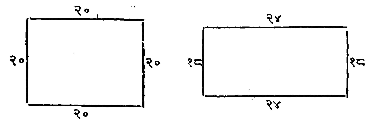
\includegraphics[width=90mm]{graphics/capture1.png}
\end{figure}

\textbf{उदाहरणम्~। }
\begin{quote}
    \bqt 
    भुजयोः पञ्चास्ये द्वौ भुव्यष्टौ द्विसमबाहुकस्याथ~।\\
\footnote{The reading त्रिसम- doesn't fit in meter.}त्रिभुजसमस्यैकादशवदने पञ्चैव भुजासु च\footnote{The reading भुजयोश्च doesn't fit in the meaning as dual case is used for three sides.}॥~२~॥ \\
चत्वारोऽस्य हि वदने भुजयोश्च सप्तपञ्च भुवि तु\footnote{The reading भुवि doesn't fit in meter.}।\\
दश वद गणितं स्थूलं यदि पटुता तेऽस्ति गणितविधौ~॥~३~॥
\end{quote}

 न्यासः~। 
 
\begin{figure}[h!]
    \centering
    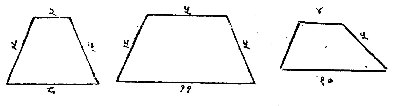
\includegraphics[width=110mm]{graphics/capture2.png}
\end{figure}
\vspace{-2mm}

 जातानि स्थूलफलानि २५। ४०। ४२~। \\
\vspace{-2mm}

\textbf{अपि च~। }
\begin{quote}
    \bqt 
    त्र्यस्रे समे दिनकरैश्च समे द्वितुल्यौ \\
    बाहू नभःकुभिरिला दिनपैः समा च~।
\end{quote}

\newpage
%%%%%%%%%%%%%%%%%%%%%%%%%%%%%%%%%%%%%%%%%%%%%%%%5
\setcounter{footnote}{0}

\begin{quote}
    \bqt 
एको भुजः कुयमलैर्विषमे परौ द्वौ \\
शैलेन्दुभिः कुपरिपूर्णकुभिः फलं किम्~॥~४~॥
\end{quote}

 न्यासः~।

\begin{figure}[h!]
    \centering
    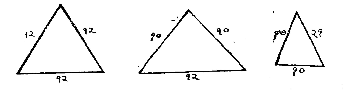
\includegraphics[width=110mm]{graphics/capture3.png}
\end{figure}

 जातानि स्थूलफलानि ७२~। ६०~। ९५~। \\

\vspace{-2mm}
\textbf{सूत्रम्~। }
\begin{quote}
    \bs 
    वृत्ते त्रिहतव्यासः परिधिः स व्यासाङ्घ्रि\footnote{The reading व्यासे परिधिर्व्यासाङ्घ्रि- neither fits in any meter nor forms a good syntactical connection.}ताडितः फलम्~।\\
व्यासवृत्तकृतित्रिघ्ने द्विवर्गषड्वर्गभक्ते च\footnote{The reading वा doesn't fit in meter.}॥~९~॥
\end{quote}

\textbf{उदाहरणम्~। }
\begin{quote}
    \bqt 
    यत्र व्यासो दश क्षेत्रे वृत्ते गणितकोविद~।\\
स्थूलं च परिधिं ब्रूहि गणितं व्यावहारिकम्~॥~५~॥
\end{quote}

 न्यासः~। 
 \vspace{-4mm}
 
\begin{table}[h!]
    \begin{tabular}{lr}
     \multirow{8}{*}{ 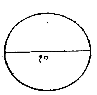
\includegraphics{graphics/capture4.png}}&  \multirow{8}{*}{जातः स्थूलपरिधिः ३०~। स्थूलफलं च ७५~। }\\
         & \\
          &  \\
          &  \\
          &  \\
          &  \\
          &  \\
          &  \\
    \end{tabular}
\end{table}
\newpage
%%%%%%%%%%%%%%%%%%%%%%%%%%%%%%%%%%%%%%
\textbf{सूत्रम्~।}
\setcounter{footnote}{0}
 \begin{quote}
     \bs 
     \footnote{अत्रोपपत्तिः~। मुखार्धरहितव्यासस्य परिधिरेव शङ्खस्य
परिधिरिति स्थूलतया दृश्यते~। तत्र त्रिघ्नो व्यासः स्थूलः परिधिरिति पूर्वं प्रतिपादितम्~। व्यासजन्यवृत्तफलं मुखदलोनव्यासमुखदलवधेन सार्धैकगुणेन हीनं शङ्खफलं भवतीति प्रत्यक्षत
आचार्येण मित्वा स्थूलं प्रकल्पितम्~। न हि शङ्खलक्षणं
विना शङ्खफलं वास्तवं न ज्ञायत इति गाणितिकैः स्फुटम्~। 
अथ यद्याचार्योक्तफलं शङ्खफलं मन्येत तर्हि तद्रूपान्तरम् 
\vspace{2mm}

\hspace{2mm} $= \mbox{३} \left\{\dfrac{\mbox{व्या}^{\text{२}}}{\mbox{४}}
  - \dfrac{\mbox{मु}}{\mbox{४}}\left(\mbox{व्या} - \dfrac{\mbox{मु}}{\mbox{२}}\right)
 \right\} = \mbox{३} \left\{\dfrac{\mbox{व्या}^{\text{२}}}{\mbox{४}}
  - \dfrac{\mbox{मु}}{\mbox{१२}}\;\mbox{३}\left(\mbox{व्या} - \dfrac{\mbox{मु}}{\mbox{२}}\right)
 \right\}$
\vspace{2mm}

\hspace{2mm} $= \mbox{३} \left(\dfrac{\mbox{व्या}^{\text{२}}}{\mbox{४}}
  - \dfrac{\mbox{मु.प}}{\mbox{१२}}\right)$
\vspace{2mm}

\hspace{2mm} अनेन प्रथमप्रकार उपपद्यते~। }मुखदलरहितो व्यासः \\
 त्रिघ्नः शङ्खे प्रजायते परिधिः~।\\
व्यासदलकृतिर्वृत्य-\\
र्कांशहतास्योनिता फलं त्रिघ्नम्~॥~१०~॥
 \vspace{1mm}
 
वदनदलोनो व्यासो \\
वदनदलं यत्तदर्धवर्गैक्यम्~।\\
त्रिगुणितमथवा गणितं \\
स्थूलं शङ्खाकृतौ भवति~॥~११~॥
 \end{quote}

\newpage%%%%%%%%%%%%%%%%%%%%%%%%%%%%%%%%%%%%%%%%%%%%

\textbf{उदाहरणम्~। }
\begin{quote}
    \bqt 
    मुखेऽष्टौ शङ्खवृत्तस्य मध्यव्यासो जिनोन्मितः~।\\
तत्र किं परिधेर्मानं फलं च वद कोविद~॥~६~॥
\end{quote}

 न्यासः~। 
 
\begin{figure}[h!]
    \centering
    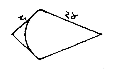
\includegraphics[width=35mm]{graphics/capture5.png}
\end{figure}

 जातः परिधिः ६०~। गणितम् ३१२~। ( वृतिरिति परिधिः )

\blfootnote{ \hspace{-4mm} अथ तदेव रूपान्तरम्\textemdash\ 
\vspace{2mm}

\hspace{4mm} $=$ ३ $\left\{\dfrac{\mbox{व्या}^{\text{२}}}{\mbox{४}}
  - \dfrac{\mbox{मु}}{\mbox{४}}\left(\mbox{व्या} - \dfrac{\mbox{मु}}{\mbox{२}}\right)
 \right\}$ 
\vspace{2mm}

\hspace{4mm} $=$ ३ $\left\{\dfrac{\mbox{व्या}^{\text{२}}}{\mbox{४}}
 - \dfrac{\mbox{मु.व्या}}{\mbox{४}} + \dfrac{\mbox{मु}^{\text{२}}}{\mbox{८}}\right\}$ 
\vspace{2mm}

\hspace{4mm} $=$ ३ $\left\{\dfrac{\mbox{व्या}^{\text{२}}}{\mbox{४}} - \dfrac{\mbox{मु.व्या}}{\mbox{४}} + \dfrac{\mbox{मु}^{\text{२}}}{\mbox{१६}} + \dfrac{\mbox{मु}^{\text{२}}}{\mbox{१६}}
 \right\}$ 
\vspace{2mm}

\hspace{4mm} $=$ ३ $\left\{\left(\dfrac{\mbox{व्या}}{\mbox{२}} - \dfrac{\mbox{मु}}{\mbox{४}}\right)^{\text{२}} +
 \left(\dfrac{\mbox{मु}}{\mbox{४}}\right)^{\text{२}}\right\}$
\vspace{2mm}

\hspace{4mm} $=$ ३ $\left[\left\{\dfrac{\mbox{१}}{\mbox{२}}\left(\mbox{व्या} - \dfrac{\mbox{मु}}{\mbox{२}}\right)\right\}^{\text{२}} + \left\{\dfrac{\mbox{१}}{\mbox{२}} - \dfrac{\mbox{मु}}{\mbox{२}}\right\}^{\text{२}}\right]$  
\vspace{2mm}

\hspace{2mm} एतेन प्रकारान्तरमुपपद्यते~। }

\newpage
%%%%%%%%%%%%%%%%%%%%%%%%%%%%%%%%%%%%%%%%%%%%
\setcounter{footnote}{0}
\textbf{ सूत्रम्~। }
\begin{quote}
    \bs 
    \footnote{अत्रोपपत्तिः~। कल्पते अ च क ग\textendash वृत्ते~ क घ ग $=$ जीवा~। 
के अ $=$ वृत्तव्यासार्धम् $=$ त्रि~। 
\begin{center}
    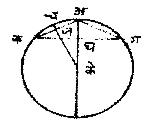
\includegraphics[scale=0.6]{graphics/capture6.png}
\end{center}

अ घ $=$ शरः~। अ ज क $=$ पूर्णज्या~। च ज के रेखा पूर्णज्यार्धकारिणी~। च ज $=$ पूर्णज्यार्धे लम्बः~। अ क घ, अ ज के\; त्रिभुजयोः साजात्यात्\, के ज $= \dfrac{\mbox{क घ\,.\,के अ}}{\mbox{अ क}} = \dfrac{\dfrac{\mbox{जी.त्रि}}{\mbox{२}}}{\mbox{पू}}$; च ज $=$ के च $-$ के ज
$= \mbox{त्रि} - \dfrac{\mbox{जी.त्रि}}{\mbox{२\,पू}} = \dfrac{\mbox{त्रि}}{\mbox{पू}}\left(\mbox{पू} - \dfrac{\mbox{जी}}{\mbox{२}}\right)$ इदं पूर्णज्यार्धगुणं च क अ त्रिभुजफलम्~। तद्द्विगुणं अ क, अ ग पूर्णज्योपरि त्रिभुजफलयोगः $= \mbox{त्रि} \left(\mbox{पू} - \dfrac{\mbox{जी}}{\mbox{२}}\right)$~। अयं अ क ग त्रिभुजफलेना\textendash \,$\dfrac{\mbox{श.जी}}{\mbox{२}}$\textendash \,नेन युतश्चापफलं स्वल्पान्तरात् 
$= \dfrac{\mbox{श.जी}}{\mbox{२}} + \mbox{त्रि} \left(\mbox{पू} - \dfrac{\mbox{जी}}{\mbox{२}}\right)$
अथ रेखागणितयुक्त्या\, त्रि $= \dfrac{\mbox{४ श}^{\text{२}} + \mbox{जी}^{\text{२}}}{\mbox{८ श}}$ अथ रेखागणित-}द्विगुणितशरशिञ्जिन्योर्यदनल्पं तद्द्विसङ्गुणं कृत्वा~।\\
अल्पायुतार्धं कोष्ठं स्वल्पाङ्घ्रिघ्नं फलं धनुषि~॥~१२~॥
\end{quote}

\newpage
%%%%%%%%%%%%%%%%%%%%%%%%%%%%%%%%%%%%%%%%%%%%
\setcounter{footnote}{0}

 \textbf{उदाहरणम्~।} 
 \blfootnote{\hspace{-4mm} युक्त्या अ क > क घ < अ घ~। च क अ त्रिभुजात् च क अ चापक्षेत्रस्याधिकत्वात्~ पू $- \dfrac{\text{जी}}{\text{२}}$ इदं शरसमं कल्पितम्~। ततो जातं धनुषः फलम् 
\vspace{2mm}

\hspace{15mm} $= \dfrac{\text{जी.श}}{\text{२}} + \dfrac{\text{४श}^{\text{२}} + \text{जी}^{\text{२}}}{\text{८श}}.$श 
\vspace{2mm}

\hspace{15mm} $= \dfrac{\text{जी.श}}{\text{२}} + \dfrac{\text{४श}^{\text{२}} + \text{जी}^{\text{२}} }{\text{८}} $ ~अत्र यदि २श > जी 
\vspace{2mm}

\hspace{15mm} $= \dfrac{\text{जी}}{\text{४}} \left\{\text{२श} + \dfrac{\text{जी}}{\text{२}} + \dfrac{\text{२श}^{\text{२}}}{\text{जी}}\right\}$ ~आचार्येण तृतीयखण्डं त्यक्तम्~। 
\vspace{2mm}

\hspace{2mm} ततो~ धफ $= \dfrac{\text{जी}}{\text{४}} \left\{\text{२श} + \dfrac{\text{जी}}{\text{२}}\right\} = \dfrac{\text{जी}}{\text{४}} \left(\dfrac{\text{४श + जी}}{\text{२}}\right)$
\vspace{2mm}

\hspace{2mm} वा,~~ धफ $= \dfrac{\text{जी.श}}{\text{२}} + \dfrac{\text{श}^{\text{२}}}{\text{२}} + \dfrac{\text{जी}^{\text{२}}}{\text{८}} = \dfrac{\text{२श}}{\text{४}} \left(\text{जी} + \text{श} + \dfrac{\text{जी}^{\text{२}}}{\text{४श}}\right)$
\vspace{2mm}

\hspace{2mm} अत्रापि तृतीयखण्डत्यागेन~ धफ $= \dfrac{\text{२श}}{\text{४}} \left(\dfrac{\text{२जी + २श}}{\text{२}}\right)$ ~यदि २श < जी~। 
\vspace{2mm}

\hspace{2mm} एवं महत्स्थूलं धनुषः फलं भवति~। सूक्ष्मार्थं पूज्यपादपितृशोधितभास्करलीलावती द्रष्टव्या~। }
\begin{quote}
    \bqt 
    मौर्व्यां\footnote{The reading मौर्व्या seems to be a typographical error.} दिशः शरे वेदाश्चापे\footnote{The reading वेदा चापे seems to be a typographical error.} कोष्ठं फलं च किम्~।\\
यत्र ज्या रविसङ्ख्या वा बाणो गजमितो वद~॥~७~॥
\end{quote}

 न्यासः~। 
 \vspace{-4mm}
 
\begin{figure}[h!]
    \centering
    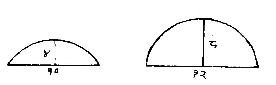
\includegraphics[scale=0.8]{graphics/capture7.png}
\captionsetup{labelformat=empty}
\end{figure}
 \vspace{-4mm}

जाते कोष्ठे १४~। २२ फले च २८~। ६६~।

\newpage%%%%%%%%%%%%%%%%%%%%%%%%%%%%%%%%%%%%%%%%%%%%
\setcounter{footnote}{0}
 \textbf{सूत्रम्~।} 
\begin{quote}
    \bs 
    गजदन्तं\footnote{अत्रोपपत्तिः~। यद्यपि गजदन्तादयो वस्तुतस्त्रिभुजादिकारा
न सन्ति तथापि स्थूलफलानयनाय तादृशा-कारास्ते कल्पिता
आचार्येण~।} त्रिकोणं स्यान्नेम्याकारं चतुर्भुजम्~।\\
बालेन्दु-यव-वज्राणां त्रिभुजद्वितयं पृथक्~॥~१३~॥\\
ढक्कायाश्च मृदङ्गस्य चतुरस्रद्वयं भवेत्~। 
\end{quote}

 \textbf{उदाहरणम्~।} 
\begin{quote}
    \bqt 
     उर्वी च पञ्चप्रमिता भुजौ तु \\
     भूपार्कसङ्ख्याविभदन्तरूपे~।\\
नेम्याकृतौ वासररन्ध्रमानौ \\
बाहू च कोटी द्विमिते फलं किम्~॥~८~॥
\end{quote}

 न्यासः~। 
 \vspace{-4mm}

\begin{figure}[h!]
    \centering
    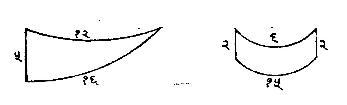
\includegraphics[scale=0.8]{graphics/capture8.png}
\captionsetup{labelformat=empty}
\end{figure}
 \vspace{-4mm}

जाते फले ३५।२४~।

\newpage
%%%%%%%%%%%%%%%%%%%%%%%%%%%%%%%%%%%%%%%%%%%%
 \textbf{अपि च~।} 
\begin{quote}
    \bqt 
    त्रिलम्बे बालशशिनि नखषोडशबाहुके~।\\
यवाकारेऽर्कलम्बे च त्रिंशद्बाहुनि किं फलम्~॥~९~॥
\end{quote}

 न्यासः~। 
\vspace{-4mm}

\begin{figure}[h!]
    \centering
    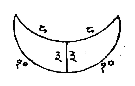
\includegraphics[scale=0.7]{graphics/capture9.png}
\end{figure}

 बालेन्दुलम्बः ३ अस्य कृते त्रिभुजे द्वे जाते फले 
 $\dfrac{\mbox{२७}}{\mbox{२}}$~। $\dfrac{\mbox{२७}}{\mbox{२}}$
अनयोर्योगो बालेन्दुफलम् २७~। \\
\vspace{-2mm}

 यवाकारं क्षेत्रम्~। 
\vspace{-4mm}

\begin{figure}[h!]
    \centering
    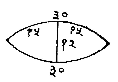
\includegraphics[scale=0.7]{graphics/capture10.png}
\end{figure}

 अस्य कृते त्रिभुजे द्वे जाते फले ९०~। ९०~। अनयोर्योगो
यवफलम् १८०~। \\

\vspace{-4mm}
 अथवास्य द्वे चापे भवतः~। तद्यथा~। भुजमानकाष्ठं लम्बार्धम् ६~। शरविलोम-विधिना जीवा~। \\

\vspace{-2mm}
 क्षेत्रदर्शनम्~। 
\vspace{-4mm}

\begin{figure}[h!]
    \centering
    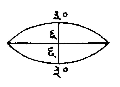
\includegraphics[scale=0.7]{graphics/capture11.png}
\captionsetup{labelformat=empty}
\end{figure}
\vspace{-4mm}

चापयोः फले ते एव ९०~। ९०

\newpage
%%%%%%%%%%%%%%%%%%%%%%%%%%%%%%%%%%%%%%%%%%%%%%%%5
 \textbf{अपि च~।} 
\begin{quote}
    \bqt 
     वज्रस्य च ढक्काया \\
     मुरजस्य च बाहवो नृपतितुल्याः~।\\
वदनानि कृतमितानि क्रमशो \\
मध्ये खचन्द्रषट्कानि~॥~१०~॥\\
गणितं यदि वेत्सि सखे \\
स्थूलं मे वृत्तजं कथय ।
\end{quote}

 न्यासः~। 
 \vspace{-4mm}

\begin{figure}[h!]
    \centering
    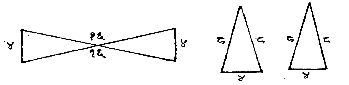
\includegraphics[scale=0.8]{graphics/capture12.png}
\end{figure}

\vspace{-2mm}
 अथ वज्रस्य कृते त्र्यस्रे जाते फले १६~। १६ अनयोरैक्यं वज्रफलम् ३२~। \\
 \vspace{-2mm}

\indent न्यासः~। 
\vspace{-2mm}

\begin{figure}[h!]
    \centering
    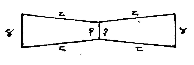
\includegraphics[scale=0.8]{graphics/capture13.png}
\captionsetup{labelformat=empty}
\end{figure}
\vspace{-2mm}

अथ ढक्काकृतिक्षेत्रस्य द्वे चतुर्भुजे भवतः~।
\vspace{-2mm}

\begin{figure}[h!]
    \centering
    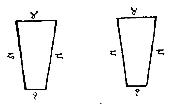
\includegraphics[scale=0.8]{graphics/capture14.png}
\captionsetup{labelformat=empty}
\end{figure}
\vspace{-2mm}

जाते क्षेत्रफले २०~। २० अनयोरैक्यं वज्रफलम् ४०~।
\newpage
%%%%%%%%%%%%%%%%%%%%%%%%%%%%%%%%%%
\setcounter{footnote}{0}
 अथ मुरजाकृतिक्षेत्रम्~। 
\vspace{-2mm}

\begin{figure}[h!]
    \centering
    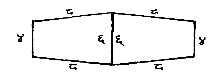
\includegraphics[scale=0.8]{graphics/capture15.png}
\captionsetup{labelformat=empty}
\end{figure}
\vspace{-2mm}

अस्य द्वे चतुर्भुजे कृते
\vspace{2mm}

 न्यासः~। 
\begin{figure}[h!]
    \centering
    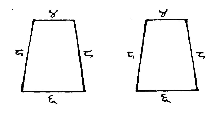
\includegraphics[scale=0.8]{graphics/capture16.png}
\end{figure}
\vspace{-2mm}

 जाते क्षेत्रफले ४०~। ४० अनयोरैक्यं मुरजाकृतिक्षेत्रफलम् ८०~। 
 \vspace{2mm}
 
 एवमन्यत्रापि यद्यदाकारं क्षेत्रं दृश्यते तत्तदाकारेण विभज्य स्वकरणेन
फलमानयेत्~। \\

\textbf{सूत्रम्~।} 
\begin{quote}
    \bs 
 \footnote{अत्रोपपत्तिः~। चक्रवृत्तयोर्मध्येऽन्तरं निर्गमसञ्ज्ञम्~। अन्तर्वृत्तस्य व्यासो मध्यसञ्ज्ञः~। द्वयोर्वृत्तयोः फलयोरन्तरं चक्रफलम्~। }निर्गमवर्गसमेता \\
  निर्गममध्याहतिस्त्रिसङ्गुणिता~।
\end{quote}
\newpage
%%%%%%%%%%%%%%%%%%%%%%%%%%%%%%%%%%%%%%%%%%%%
\begin{quote}
    \bs 
 चक्राकृतिनि फलं स्यात् \\
 रथाङ्गशकलं तु नेमिरिह~॥~१४~॥ 
\end{quote}
\blfootnote{\hspace{-4mm} अन्तर्वृत्तपरिधिः $=$ ३\,म, तत्फलम् $\dfrac{\mbox{३\,म}^{\text{२}}}{\mbox{४}}$, बहिर्वृत्तपरिधिः $=$ ३\,(म $+$ २\,नि),
 \vspace{1mm}
 
तत्फलम् $= \dfrac{\mbox{३}}{\mbox{४}} (\mbox{म + २\,नि})^{\text{२}},$
 \vspace{2mm}
 
\hspace{2mm} द्वयोरन्तरं चक्रफलम् $= \dfrac{\mbox{३}}{\mbox{४}}\left\{(\mbox{म + २\,नि})^{\text{२}} - \mbox{म}^{\text{२}}\right\}$
  \vspace{2mm}

\hspace{2.7cm} $= \dfrac{\mbox{३}}{\mbox{४}}\,(\mbox{४\,म.नि + ४\,नि}^{\text{२}})$
 \vspace{1mm}

\hspace{2.7cm} $= \mbox{३}\,(\mbox{म.नि + नि}^{\text{२}})~।$ 
 \vspace{1mm}

\hspace{2mm} अथान्तर्वृत्तपरिधिः $=$ ८ $\times$ ३ $=$ २४~ प्रथमरथाङ्गमानम्~।
 \vspace{1mm}

\hspace{2mm} बहिर्वृत्तपरिधिः $=$ ३ (८ $+$ २\,नि) $=$ ३६~ द्वितीयरथाङ्गमानम्~। 
 \vspace{1mm}

\hspace{2mm} द्वयोर्योगार्धसमा नेमिः $=$ ३० कल्पिताचार्येण~।}
 \textbf{उदाहरणम्~।} 
\begin{quote}
    \bqt 
    रथाङ्गतिस्तले\footnote{The reading रथाङ्गमिस्तले seems to be a typographical error.} नाभावष्टौ युग्मं च निर्गमे~।\\
तत्र किं गणितं ब्रूहि सखे मे व्यावहारिकम्~॥~११~॥
\end{quote}

 न्यासः~। 
 \vspace{-2mm}

\begin{figure}[h!]
    \centering
    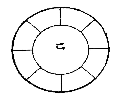
\includegraphics[scale=0.8]{graphics/capture17.png}
\end{figure}
\vspace{-2mm}

 फलम् ६०~। अस्य शकलं नेमिः~। 
\newpage%%%%%%%%%%%%%%%%%%%%%%%%%%%%%%%%%%%%%%%%%%%%
\setcounter{footnote}{0}
 \textbf{सूत्रम्~।} 
\begin{quote}
    \bs 
    \footnote{त्रिभुजे रश्मित्रयम्~। चतुर्भुजे रश्मिचतुष्टयम्~। एवं प्रतिक्षेत्रं भुजसङ्ख्यासमं रश्मिमानम्~। समत्रिभुजे प्रथमं रूपसमा
भुजाः कल्पिताः~। तदा भुजप्रतिभुजयोगः $=$ र$-$१, अन्यभुजः 
$= \dfrac{\mbox{र}}{\mbox{३}}$~। '\hyperref[4.8]{प्रतिभुजभुजतद्युतिदले}' इत्यादि ८ सूत्रेण त्रिभुजस्य
स्थूलं फलम् $= \dfrac{\mbox{र} - \mbox{१}}{\mbox{२}} \times \dfrac{\mbox{र}}{\mbox{६}} = \dfrac{\mbox{र}^{\text{२}} - \mbox{र}}{\mbox{६}}$~। ततो रेखागणितषष्ठाध्यायेन यस्य समत्रिभुजस्य भुजमानम् $=$ भु, तस्य फलम्
$= \mbox{भु}^{\text{२}} \dfrac{\mbox{र}^{\text{२}} - \mbox{र}}{\mbox{१२}}$~। अतस्त्रिभुजफलानयनमुपपद्यते~। 
वर्गक्षेत्रे रूपतुल्यभुजे भुजत्रययोगः $=$ र$-$१~। एकभुजमानम्
$= \dfrac{\mbox{र} - \mbox{१}}{\mbox{३}} ,\ \dfrac{\mbox{र}}{\mbox{४}}$~। अनयोर्वधः $= \dfrac{(\mbox{र} - \mbox{१})\,\mbox{र}}{\mbox{१२}}= \dfrac{\mbox{र}^{\text{२}} - \mbox{र}}{\mbox{१२}} =$ रूपभुजवर्गक्षेत्रस्य फलम्~। इदमिष्टभुजवर्गगुणमभीष्टवर्गफलम् $= \dfrac{\mbox{भु}^{\text{२}}(\mbox{र}^{\text{२}} - \mbox{र})}{\mbox{१२}}$~। अथ यद्येवं पञ्चभुजं समं भवेत् यत्र 
\vspace{-6mm}

\begin{center}
    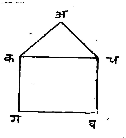
\includegraphics[scale=0.7]{graphics/capture18.png}
\end{center}
\vspace{-4mm}

\noindent अ क च समत्रिभुजं, क ग घ च वर्गक्षेत्रं तदा पूर्वप्रकारेण रूपभुजसमे समत्रिभुजे रश्मिमानम् $= \dfrac{\mbox{३\,र}}{\mbox{५}}$~। रूपसमभुजवर्गक्षेत्रे रश्मि\textendash}रश्म्यूनरश्मिकृतिहत-\\
भुजकृतिरिनहृत् फलं त्रिकोणादौ~॥~१५~॥
\end{quote}
 
\newpage%%%%%%%%%%%%%%%%%%%%%%%%%%%%%%%%%%%%%%%%%%%%
 \textbf{उदाहरणम्~।} 
\begin{quote}
    \bqt 
    त्रिरश्म्यादिषडस्रान्तक्षेत्राणां वद कोविद~।\\
फलं षट्-सङ्ख्यबाहूनां गणिते कुशलोऽसि चेत्~॥~१२~॥
\end{quote}

 न्यासः~। 
 \vspace{-2mm}
 
\begin{figure}[h!]
    \centering
    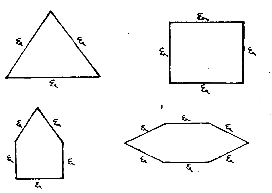
\includegraphics[scale=0.8]{graphics/capture19.png}
\end{figure}
 \vspace{-2mm}

 जातानि फलानि १८~। ३६~। ६०~। ९०\blfootnote{
\hspace{-10mm} मानम् $= \dfrac{\mbox{४\,र}}{\mbox{५}}$~। ततो द्वयोः फले $\dfrac{\mbox{९\,र}^{\text{२}} - \mbox{१५\,र}}{\mbox{२५} \times \mbox{१२}} ,~
\dfrac{\mbox{१६\,र}^{\text{२}} - \mbox{२०\,र}}{\mbox{२५} \times \mbox{१२}}$
द्वयोर्योगः रूपसमभुजपञ्चभुजफलम् $= \dfrac{\mbox{२५\,र}^{\text{२}} - \mbox{३५\,र}}{\mbox{१२} \times \mbox{२५}} = \dfrac{\mbox{र}^{\text{२}} - \mbox{र}}{\mbox{१२}}$
स्थूलात्~। अभीष्टपञ्चभुजफलम् $= \dfrac{\mbox{भु}^{\text{२}}}{\mbox{१२}}(\mbox{र}^{\text{२}} - \mbox{र})$~। एवमत्र
कस्यचित् समपञ्चभुजक्षेत्रस्य फल\textendash \,$\dfrac{\mbox{भु}^{\text{२}}}{\mbox{१२}} (\mbox{र}^{\text{२}} - \mbox{र})$\textendash \,मिति भवति~। 
एवं क्षेत्रयुक्त्या समषडस्रे षडस्रमध्यात् कोणगरेखाभिः षट् समत्रिभुजानि प्रकल्प्याचार्योक्तस्थूलप्रकारेणैव त्रिभुजफलमानीय
तत् षड्गुणं षडस्रफलं साध्यते तदा फलम् $= \mbox{भु}^{\text{२}} \bigg(\dfrac{\mbox{३\,र}^{\text{२}} - \mbox{६\,र}}{\mbox{२} \times \mbox{१२}}\bigg)$
एतस्य स्थाने आचार्येण\; 
$\mbox{भु}^{\text{२}}\ \dfrac{\mbox{(र}^{\text{२}} - \mbox{र)}}{\mbox{१२}}$\;
 इदं गृहीतम्~। एवमत्र 
वर्गक्षेत्रमपहाय सर्वत्रैव स्थूलतेति स्फुटम्~। }

\newpage%%%%%%%%%%%%%%%%%%%%%%%%%%%%%%%%%%%%%%%%%%%%

 अथ करणम्~। त्र्यस्रिक्षेत्रे रश्मिः ३ अस्य कृतिः ९ रश्म्यूना ६
अनया भुजस्यास्य कृतिः ३६ हता २१६~। द्वादशभक्ता जातं 
त्र्यस्रक्षेत्रफलम् १८~। एवमन्येषां चतुर्भुजादीनामपि~।\\

 \textbf{सूत्रम्~।} 
\begin{quote}
    \bs 
    \footnote{अत्रोपपत्तिः~। 
 \vspace{1mm}

\hspace{4mm} रश्म्यूनरश्मीत्यादिना त्रिभुजफलम् $= \dfrac{(\mbox{र}^{\text{२}} - \mbox{र})~\mbox{भु}^{\text{२}}}{\mbox{१२}} = \dfrac{(\mbox{र} - \mbox{१})\,\mbox{र}^{\text{२}} \times \mbox{भु}^{\text{२}}}{\mbox{३} \times \mbox{र} \times \mbox{४}}$~। 
 \vspace{2mm}

\hspace{4mm} अथ वृत्तखण्डत्रयफलयोगः $=  \dfrac{\mbox{३भु}^{\text{२}}}{\mbox{८}} = \dfrac{\mbox{३} \times \mbox{भु}^{\text{२}}\,(\mbox{र} - \mbox{१}) \times \mbox{र}^{\text{२}}}{\mbox{र}^{\text{२}} \times \mbox{८} \times (\mbox{र} - \mbox{१})}$ 
 \vspace{2mm}

\hspace{4mm} अनयोरन्तरं वृत्तान्तः क्षेत्रफलम् $=
\dfrac{(\mbox{र} - \mbox{१})\,\mbox{र}^{\text{२}} \times \mbox{भु}^{\text{२}}}{\mbox{३} \times \mbox{र} \times \mbox{४}}\ -\ 
\dfrac{\mbox{३} \times \mbox{भु}^{\text{२}}\,(\mbox{र} - \mbox{१})\,\mbox{र}^{\text{२}}}{\mbox{र}^{\text{२}} \times \mbox{८} \times (\mbox{र} - \mbox{१})}$ 
 \vspace{2mm}

\hspace{40mm} $= \dfrac{(\mbox{र} - \mbox{१})\,\mbox{र}^{\text{२}} \times \mbox{भु}^{\text{२}}}{\mbox{४}}\ \Bigg\{\dfrac{\mbox{१}}{\mbox{३} \times \mbox{र}} - \dfrac{\mbox{३}}{\mbox{र}^{\text{२}} \times (\mbox{र} - \mbox{१}) \times \mbox{२}}\Bigg\}$ 
 \vspace{2mm}

\hspace{4mm} अत्र यदि स्वल्पान्तरात् \hspace{8mm} $= \dfrac{\mbox{१}}{\mbox{३} \times \mbox{र}} - \dfrac{\mbox{३}}{\mbox{र}^{\text{२}} \times (\mbox{र} - \mbox{१}) \times \mbox{२}} = \dfrac{\mbox{१}}{\mbox{र} \times \mbox{९}}$}व्याससमासार्धकृतिः\\
 निरेकवृत्ताहता हृता वृत्तैः~।\\
नवगुणितैर्वृत्तान्तर-\\
फलमथवा रश्मिजं त्रिहृतम्~॥~१६~॥
\end{quote}
\newpage%%%%%%%%%%%%%%%%%%%%%%%%%%%%%%%%%%%%%%%%%%%%

 \textbf{उदाहरणम्~।} 
\begin{quote}
    \bqt 
    द्वादशविष्कम्भाणाम् \\
    अन्योन्यश्लिष्टवृत्तानाम्~।
\end{quote}
 \blfootnote{ 
\hspace{-4mm} तदा~। 
 \vspace{2mm}

\hspace{4mm} $\dfrac{(\mbox{र} - \mbox{१})\,\mbox{र}^{\text{२}} \times \mbox{भु}^{\text{२}}}{\mbox{४}} \times \dfrac{\mbox{१}}{\mbox{९} \times \mbox{र}} =$ क्षेत्रफलम्~। 
 \vspace{2mm}

\hspace{4mm} अत्र यतः~। $\dfrac{\mbox{व्याससमासः}}{\mbox{२}} = \dfrac{\mbox{र} \times \mbox{भु}}{\mbox{२}}$~। $\Bigg(\dfrac{\mbox{व्या.}\mbox{स}}{\mbox{२}}\Bigg)^{\text{२}}
 = \dfrac{\mbox{र}^{\text{२}}\times \mbox{भु}^{\text{२}}}{\mbox{४}}$~। वृत्तसङ्ख्या $=$ र~।
 \vspace{2mm}

\hspace{4mm} ततः क्षेत्रफलम् $= \dfrac{\bigg(\dfrac{\mbox{व्या.स}}{\mbox{२}}\bigg)^{\text{२}}\ (\mbox{वृ\,सं} - \mbox{१})}{\mbox{वृ.सं} \times \mbox{९}}$ अत उपपद्यत इति~। 
 \vspace{2mm}

\hspace{4mm} एवमत्र चतुर्वृत्तान्तः फलम् 
$= \dfrac{(\mbox{र} - \mbox{१})\,\mbox{र}^{\text{२}} \times \mbox{भु}^{\text{२}}}{\mbox{४}}\ \Bigg\{\dfrac{\mbox{१}}{\mbox{३} \times \mbox{र}} - \dfrac{\mbox{३}}{\mbox{र}^{\text{२}}\ (\mbox{र} - \mbox{१})}\Bigg\}$
 \vspace{2mm}

\hspace{8mm} अत्रापि~~
 $\dfrac{\mbox{१}}{\mbox{३} \times \mbox{र}} - \dfrac{\mbox{३}}{\mbox{र}^{\text{२}}\ (\mbox{र} - \mbox{१})} = \dfrac{\mbox{१}}{\mbox{र} \times \mbox{९}}$
 \vspace{2mm}

\hspace{4mm} उत्थापनात् क्षेत्रफलम् $= \dfrac{ \Bigg(\dfrac{\mbox{व्यास}}{\mbox{२}}\Bigg)^{\text{२}} \times (\mbox{वृ\,सं} - \mbox{१})}{\mbox{वृ\,सं} \times \mbox{९}}$
 \vspace{1mm}

\hspace{4mm} एवं समपञ्चास्रादिषु~। 
 \vspace{1mm}

\hspace{4mm} अथ पूर्वफलम् $= \dfrac{(\mbox{र} - \mbox{१})\ \mbox{र}^{\text{२}} \times \mbox{भु}^{\text{२}}}{\mbox{४} \times \mbox{९} \times \mbox{र}}= \dfrac{\mbox{(र}^{\text{२}} - \mbox{र})\ \mbox{भु}^{\text{२}}}{\mbox{४} \times \mbox{३} \times \mbox{३}}$
 \vspace{2mm}

\hspace{4mm} अत्र त्रिकोणादिफलम् $= \dfrac{(\mbox{र}^{\text{२}} - \mbox{र})\ \mbox{भु}^{\text{२}}}{\mbox{४} \times \mbox{३}}$~। 
 \vspace{2mm}

\hspace{4mm} ततः~~ $\dfrac{\mbox{रश्मिजत्रिकोणादिफ}}{\mbox{३}} =$ इष्टक्षेत्रफलम्~। }
\newpage
%%%%%%%%%%%%%%%%%%%%%%%%%%%%%%%%%%%%%%%%%
\begin{quote}
    \bqt 
त्र्यादिषडन्तानां \\
वद वृत्तानामन्तरालफलम्~॥~१३~॥
\end{quote}

 न्यासः~। 
 \vspace{-2mm}
 
\begin{figure}[h!]
    \centering
    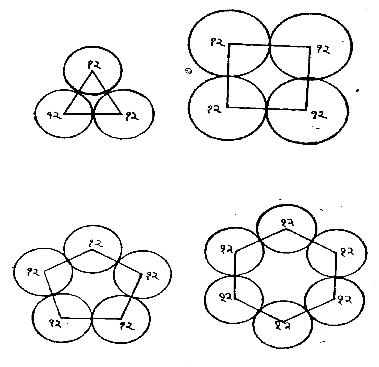
\includegraphics[scale=0.65]{graphics/capture20.png}
    \captionsetup{labelformat=empty}
\end{figure}
 \vspace{-2mm}

जातानि वृत्तान्तरफलानि २४~। ४८~। ८०~। १२०~।
\newpage
%%%%%%%%%%%%%%%%%%%%%%%%%%%%%%%%%%%%%%%%%%%%%

 \textbf{सूत्रम्~।} 
\setcounter{footnote}{0}
\begin{quote}
    \bs 
     \footnote{अत्रोपपत्तिः~। अथाचार्यगृहीतस्थूलपरिधिः $=$ ३\,व्या $=$ परिधिः~। 
\vspace{1mm}

\hspace{4mm} तदा भास्करोक्त्या वृत्तफलम् $= \dfrac{\mbox{व्या} \times \mbox{व्या} \times \mbox{३}}{\mbox{४}} =
\dfrac{\mbox{व्या}^{\text{२}} \times \mbox{३}}{\mbox{४}} $
\vspace{2mm}

\hspace{4mm} समगुणनादिना~। 
$\dfrac{\mbox{फ} \times \mbox{४}}{\mbox{३}} = \mbox{व्या}^{\text{२}} = \mbox{फ} + \dfrac{\mbox{फ}}{\mbox{३}}$ 
\vspace{2mm}

\hspace{4mm} मूलेन~~ $\mbox{व्या} = \sqrt{\mbox{फ} + \dfrac{\mbox{फ}}{\mbox{३}}}$}गणितात् स्वत्र्यंशयुतात् \\
मूलं समवर्तुलव्यासः~॥~१७~॥
\end{quote}

 \textbf{उदाहरणम्~।} 
\begin{quote}
    \bqt 
    अशीतिर्यत्र पञ्चोना समवृत्ते फलं सखे~।\\
तत्र वृत्तप्रमाणं किं यदि वेत्सि द्रुतं वद~॥~१४~॥
\end{quote}
 
 न्यासः~। 
 \vspace{-4mm}

\begin{figure}[h!]
    \centering
    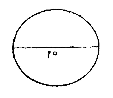
\includegraphics[scale=0.8]{graphics/capture21.png}
    \captionsetup{labelformat=empty}
\end{figure}
 \vspace{-4mm}

समवृत्तफलम् ७५~। जातो व्यासः १०~।
\newpage%%%%%%%%%%%%%%%%%%%%%%%%%%%%%%%%%%%%%%%%%%%%

 \textbf{सूत्रम्~।} 
\begin{quote}
    \bs 
    \footnote{अत्रोपपत्तिः~। ११ सूत्रोक्तशङ्खक्षेत्रफलम् $= \mbox{३}\,\Bigg[\bigg\{\dfrac{\mbox{१}}{\mbox{२}}\bigg(\mbox{व्या} - \dfrac{\mbox{मु}}{\mbox{२}}\bigg)\bigg\}^{\text{२}} + \bigg\{\dfrac{\mbox{१}}{\mbox{२}} \times \dfrac{\mbox{मु}}{\mbox{र}}\bigg\}^{\text{२}}\Bigg]$ 
\vspace{2mm}

\hspace{4mm} समभागेन~ $\Bigg\{\dfrac{\mbox{१}}{\mbox{२}}\,\bigg(\mbox{व्या} - \dfrac{\mbox{मु}}{\mbox{२}}\bigg)\Bigg\} + \bigg(\dfrac{\mbox{१}}{\mbox{२}} \times \dfrac{\mbox{मु}}{\mbox{२}}\bigg)^{\text{२}} = \dfrac{\mbox{फ}}{\mbox{३}}$ 
\vspace{2mm}

\hspace{4mm} अत्र भास्करीयमूलानयनोक्त्या प्रथमखण्डमूलम् $=$ $\dfrac{\mbox{१}}{\mbox{२}} \bigg(\mbox{व्या} - \dfrac{\mbox{मु}}{\mbox{२}}\bigg)$ 
\vspace{2mm}

\hspace{4mm} शेषमूलं च $=$ $\dfrac{\mbox{१}}{\mbox{२}} \times \dfrac{\mbox{मु}}{\mbox{२}}$ 
\vspace{2mm}

\hspace{4mm} द्वाभ्यां गुणिते मूलद्वये~। $\dfrac{\mbox{मु}}{\mbox{२}} =$ शेमू $\times$ २ $=$ लघुफल 
\vspace{2mm}

\hspace{4mm} प्रथ.\,खं.\,मू $\times$ २ $=$ व्या $- \dfrac{\mbox{मु}}{\mbox{२}} =$ अलघु 
\vspace{1mm}

\hspace{4mm} अतोऽग्रे स्फुटमिति~।  
\vspace{1mm}

\hspace{4mm} यत्र फलम् $=$ ७५~। तदा\; $\dfrac{\mbox{फ}}{\mbox{३}} =$ २५  
\vspace{2mm}

\hspace{4mm} अत्र मूलग्रहणे शेषाभावस्ततो व्यासमुखज्ञानं कष्टमेवमनेकात्र 
खण्डनम्~। किं लिखनप्राचुर्येणेति~। }त्रिहृतान्मूलं शेषं \\
शेषान्मूलं च ते पदे द्विगुणे~॥~१८~॥\\
अलघुयुतलघुर्व्यासो\footnote{The reading -लघुव्यासो seems to be a typographical error.} \\
वदनं शङ्खे लघु द्विगुणम्~।
\end{quote}
\newpage%%%%%%%%%%%%%%%%%%%%%%%%%%%%%%%%%%%%%%%%%%%%
 \textbf{उदाहरणम्~।} 
\begin{quote}
    \bqt 
    सखे शङ्खफलं षष्टिर्यत्र तत्र वद द्रुतम्~।\\
व्यासं च वदनं तेऽस्ति गणिते यदि पाटवम्~॥~१५~॥
\end{quote}

 न्यासः~। 
\vspace{-2mm}

\begin{figure}[h!]
    \centering
    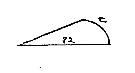
\includegraphics[scale=0.8]{graphics/capture22.png}
\end{figure}
\vspace{-6mm}

 शङ्खफलम् ६० जातो व्यासः १२ मुखम् ८~। \\

 \textbf{सूत्रम्~।} 
\setcounter{footnote}{0}
\begin{quote}
    \bs 
    \footnote{अत्र १५ सूत्रोक्तफलवैपरीत्यादुपपत्तिः स्फुटेति~। }रश्म्यूनरश्मिवर्गो- \\
    द्धृतात् फलात् रविहतात् पदं बाहुः~॥~१९~॥
\end{quote}
 \vspace{2mm}
 
 \textbf{उदाहरणम्~।} 
\begin{quote}
    \bqt
     त्रिभुजेऽष्टौ चतुरस्रे \\
     तत्त्वानि च पञ्चरश्मिके षष्टिः~।\\
षड्रश्मिके\footnote{The reading षड्राशिके seems to be a typographical error.} द्विगुणिता \\
विंशद्गणितं भुजान् कथय~॥~१६~॥
\end{quote}

\newpage%%%%%%%%%%%%%%%%%%%%%%%%%%%%%%%%%%%%%%%%%%%%

न्यासः~। समत्र्यस्रादीनां फलानि ८~। २५~। ६०~। ४०~। \\
\indent जातानि समत्र्यस्रादीनां भुजमानानि ४~। ५~। ६~। ४~। \\
 
\vspace{-2mm}
 क्षेत्रदर्शनम्~। 
\vspace{-2mm}

\begin{figure}[h!]
    \centering
    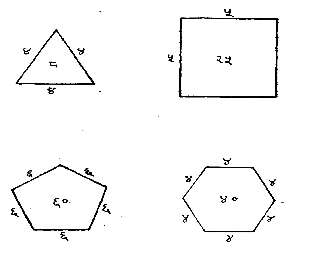
\includegraphics[scale=0.7]{graphics/capture23.png}
\end{figure}
\vspace{2mm}

\textbf{परिभाषितम् \textendash } 
\begin{quote}
    \bs 
     यैर्यैः सूत्रैर्यद्यत् \\
     फलमुपपन्नं विलोमतस्तैस्तैः~।\\
यदविज्ञातं\footnote{The reading यदि विज्ञातं seems to be a typographical error.} ज्ञेयं \\
विस्तृतिभीत्या मया नोक्तम्~॥~२०~॥
\end{quote}

\newpage
%%%%%%%%%%%%%%%%%%%%%%%%%%%%%%%%%%%%%%%%%%%%%%%
\setcounter{footnote}{0}
 \textbf{अथ सूत्रम्~।} 
\begin{quote}
    \bs 
    \footnote{भूखण्डयोगेन भूखण्डमानयोगेन ताडितं हतं यद्भूमुखयोर्विवरमन्तरं तस्मिन्~। 
\vspace{1mm}

\hspace{4mm} अत्रोपपत्तिस्त्रैराशिकेन स्फुटा~।}भूखण्डयोगगुणिते\footnote{The reading ताडिते doesn't fit in meter.} \\
 भूमुखविवरे\footnote{The reading विविरे seems to be a typographical error.} च पार्श्वयोगहृते~।\\
प्रचयः क्रमशो निजनिज-\\
मुखयुक्ता मध्यभूम्यः स्युः~॥~२१~॥
\end{quote}
 
 \textbf{उदाहरणम्~।} 
\begin{quote}
    \bqt 
    क्षेत्रस्य यस्य वदनं शशिसम्मितं भूः \\
    शैलोन्मिता त्रिगुणिताष्टमितौ च बाहू~।\\
खण्डेषु षट्सु वद मध्यतलानि बाहु-\\
खण्डे पयोनिधिमितेऽत्र पृथक् फलं किम्~॥~१७~॥
\end{quote}

 न्यासः~। खण्डभुजः ४ जातः प्रचयः १~। \\
\indent अतो जाता मध्यभूम्यः २~। ३~। ४~। ५~। ६~। \\
\indent जातानि पृथक् फलानि ६~। १०~। १४~। १८~। २२~। २६~। \\
\indent एषां फलानामैक्यं समस्तक्षेत्रफलम् ९६~। 

\newpage%%%%%%%%%%%%%%%%%%%%%%%%%%%%%%%%%%%%%%%%%%%%

 क्षेत्रदर्शनम्~। 
\vspace{-2mm}

\begin{figure}[h!]
    \centering
    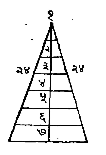
\includegraphics[scale=0.7]{graphics/capture24.png}
\end{figure}

 \textbf{अपि च~।} 
\begin{quote}
    \bqt 
     वक्त्रं च लोचनमितं तलमङ्कमानं \\
     बाहू पयोनिधिमहीधरघाततुल्यौ~।\\
स्तम्बेरमक्षितिपवारिधयो मुखादेः \\
खण्डानि मे प्रवद मध्यमहीतलानि~॥~१८~॥
\end{quote}

 न्यासः~। वदनाद्भुजखण्डानि ८~। १६~। ४ जाते मध्यभूमाने
४~। ८ फलानि च २४~। ९६~। ३४ एषामैक्यं सर्वफलम् १५४~। \\

\vspace{-2mm}
 क्षेत्रदर्शनम्~। 
\vspace{-2mm}

\begin{figure}[h!]
    \centering
    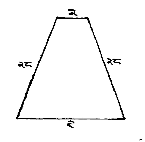
\includegraphics[scale=0.7]{graphics/capture25.png}
\end{figure}

\newpage
%%%%%%%%%%%%%%%%%%%%%%%%%%%%%%%%%%%%%%%
 \textbf{अपि च~।} 
\begin{quote}
    \bqt 
     भूमिः कुञ्जरसम्मिता च वदनं \\
     नेत्राङ्कितं षण्मितौ \\
     बाहू रन्ध्रनगाहतावथ तलात् \\
     खण्डस्य बाहू च तौ~।\\
रन्ध्राद्रिप्रमितौ पृथग्द्विगुणितौ \\
त्रिघ्नौ च खण्डत्रये \\
किं स्यान्मध्यतलं वदाशु सुमते \\
जानासि पाटीं यदि~॥~१९~॥
\end{quote}

 न्यासः~। अधस्तलाद्भुजखण्डे ९\;।\;७ मध्याद्भुजखण्डे १८\;।\;१४
उपरितने भुजखण्डे २७~। २१ तलमध्यजे जाते भूमी ७~। ५ जातानि 
फलानि ८४~। ९६~। २० ऐक्यम् २४०~। \\

\setcounter{footnote}{0}
 \textbf{सूत्रम्~।} 
\begin{quote}
    \bs 
    \footnote{युतिः खण्डफलानां योगः~। तया भूर्मुखं चेति
द्वयमुद्धृतम्~। फलद्वयदलकृत्यन्तरं यत् तेन आहतं खण्डगणितं युतिहृतभूमुखदलकृति\textendash \,इति पाठः साधुः~। }भुजयोगोद्धृतभूमुख-\\
विवराहतखण्डगणितसंयुक्तात्~।\\
मुखदलवर्गान्मूलं \\
द्विहतं तत्खण्डके\footnote{The reading द्विगुणिततत्खण्डके doesn't give a correct meaning.} भूमिः~॥~२२~॥
\end{quote}
 
\newpage%%%%%%%%%%%%%%%%%%%%%%%%%%%%%%%%%%%%%%%%%%%%
\begin{quote}
    \bs 
     भूमुखविवरविभक्तौ \\
     बाहू खण्डास्यतलवियोगघ्नौ~।\\
स्थूले वापि च सूक्ष्मे \\
तत्खण्डे बाहुमाने स्तः~॥~२३~॥
\end{quote}
\blfootnote{\hspace{-8mm} खण्डफलं तेन संयुक्तान्मुखार्धस्य वर्गान्मूलं द्विगुणितं तदा तत्खण्डे भूमिः स्यादित्यर्थः~। 
\vspace{1mm}

\hspace{2mm} अत्रोपपत्तिः~। खण्डफलानां योगः $=$ यु $=$ सम्पूर्णसमानलम्बक्षेत्रस्य फलम्~। ततो विलोमविधिना तत्समानलम्बक्षेत्रस्य
लम्बः $=$ लं $= \dfrac{\mbox{२\,यु}}{\mbox{मु} + \mbox{भू}}$~। अथ खण्डफलस्य समानलम्बक्षेत्रस्य फलम् $=$ 
ख फ, तथा तद्भूमिः $=$ य तदा तल्लम्बोऽनुपातेन $\dfrac{\mbox{२\,यु}\,(\mbox{य} - \mbox{मु})}{(\mbox{भू} + \mbox{मु})\,(\mbox{भू} - \mbox{मु})}$
{\color{violet}भास्करस्य 'लम्बेन निघ्नं कुमुखैक्यखण्डम्'} इत्यनेन तत्फलम् $=$
\vspace{2mm}

\hspace{4.5mm} $\mbox{ख फ} = \dfrac{\mbox{यु}\,(\mbox{य}^{\text{२}} - \mbox{मु}^{\text{२}})}{\mbox{भू}^{\text{२}} - \mbox{मु}^{\text{२}}}$
\vspace{2mm}

\hspace{4mm} $\therefore\; \mbox{य}^{\text{२}} = \dfrac{\mbox{ख फ}\,(\mbox{भू}^{\text{२}} - \mbox{मु}^{\text{२}})}{\mbox{यु}} + \mbox{मु}^{\text{२}}$
\vspace{2mm}

\hspace{4mm} वा~~ $\dfrac{\mbox{य}^{\text{२}}}{\mbox{४}}= \mbox{ख}\,\bigg(\dfrac{\mbox{भू}^{\text{२}}}{\mbox{४\,यु}} - \dfrac{\mbox{मुु}^{\text{२}}}{\mbox{४\,मु}}\bigg) + \dfrac{\mbox{मुु}^{\text{२}}}{\mbox{४}}$~। अत उपपन्नं
प्रथमं सूत्रम्~। 
\vspace{2mm}

\hspace{2mm} द्वितीयसूत्रस्य त्रैराशिकेन स्फुटा वासना~। }
 \textbf{उदाहरणम्~।} 
\begin{quote}
    \bqt 
    भूर्दिङ्मिता\footnote{The reading भू दिङ्मिता seems to be a typographical error.} वदनमब्धिमितं च बाहू \\
    तर्काहताम्बुधिमितौ च फलानि चास्य~।
\end{quote}

\newpage%%%%%%%%%%%%%%%%%%%%%%%%%%%%%%%%%%%%%%%%%%%%
\begin{quote}
\bqt 
दिग्वासवस्मृतिमितानि कृताहतानि \\
खण्डे त्रये कथय मध्यभुजौ भुजौ च~॥~२०~॥
\end{quote}

 न्यासः~। 
\vspace{-2mm}

\begin{figure}[h!]
    \centering
    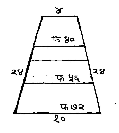
\includegraphics[scale=0.8]{graphics/capture26.png}
\end{figure}
\vspace{-2mm}

 जाते मध्यतले ६~। ८ खण्डत्रये समभुजमानम् ८~। \\
\vspace{-2mm}
 
\textbf{अपि च~।} 
\begin{quote}
    \bqt 
भूमिः कुञ्जरसम्मिता च वदनं \\
नेत्राङ्कितं तद्भुजौ \\
रन्ध्राद्रिप्रमितौ पृथग्रसहतौ \\
शैलेभबाणैः पृथक्~।\\
निघ्नान्यर्कमितानि खण्डगणिता-\\
न्याशु प्रचक्ष्वासि मां \\
खण्डेषु त्रिषु मध्यभूतलमिती \\
तद्दोः प्रमाणे वद~॥~२१~॥
\end{quote}

\newpage
%%%%%%%%%%%%%%%%%%%%%%%%%%%%%%%%%%%%%%%%%%
 न्यासः~। 
\vspace{-2mm}

\begin{figure}[h!]
    \centering
    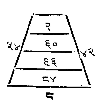
\includegraphics[scale=0.8]{graphics/capture27.png}
\end{figure}
\vspace{-3mm}

 जाते मध्यतले ५\;।\;७ तलखण्डस्यास्य पार्श्वभुजौ ९\;।\;७
मध्यखण्डस्य पार्श्वभुजौ २७\;।\;२१ मुखखण्डस्य पार्श्वभुजौ
१८\;।\;१४~। 
\vspace{2mm}

\begin{quote}
    \bs 
     पूर्वेषां गणकानाम् \\
     अनवज्ञार्थं समीरितं स्थूलम्~।\\
अत्यादरो न मेऽत्र \\
क्वचित् फलानां विसंवादात्~॥~२२~॥
\end{quote}

 \textbf{तदुदाहरणम्~।} 
\begin{quote}
    \bqt 
     खाङ्गाग्निभिर्गजगुणैश्च धरे च लम्बौ\footnote{The reading धरावलम्बौ seems to be a typographical error as it doesn't give a correct meaning.} \\
     तुल्यौ निधिक्षितिभिरम्बरकुम्भिभूभिः~।\\
क्षेत्रद्वयेऽपि च भुजौ कुगजेन्दुभिर्भोः \\
स्थूले फलादरमनादरमत्र पश्य~॥~२३~॥
\end{quote}
\newpage
%%%%%%%%%%%%%%%%%%%%%%%%%%%%%%%%%%%%%%%%%%%%%%%%%%%%
 न्यासः~। \\
\indent क्षेत्रदर्शनम्~। 
 \vspace{-2mm}
 
 \begin{figure}[h!]
    \centering
  \captionsetup{labelformat=empty}
 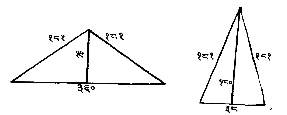
\includegraphics[scale=0.8]{graphics/capture28.png}
\end{figure}
 \vspace{-2mm}

\setcounter{footnote}{0}
 जाते स्थूलफले\footnote{अत्रास्याध्यायस्याष्टमसूत्रेण "\hyperref[4.8]{प्रतिभुजभुजतद्युतिदल}"
इत्यादिना 
 \vspace{2mm}

\hspace{6mm} प्रथमत्रिभुजे फलम् $=
\bigg(\dfrac{\mbox{१८१} + \mbox{१८१}}{\mbox{२}}\bigg)\ \bigg(\dfrac{\mbox{०} + \mbox{३६०}}{\mbox{२}}\bigg)$
$=$ १८१ $\times$ १८० $=$ ३२५८०~।
 \vspace{1mm}

\hspace{6mm} एवं द्वितीयत्रिभुजस्य फलम् $=$
१८१ $\times$ १९ $=$ ३४३९~। } ३२५८०~। ३४३९ अनयोरेकस्मादन्यं नवगुणाधिकमस्ति~। अतः फलविसंवादः~। पारमार्थिके सूक्ष्मफले
समे एव ३४२०~। ३४२०~। 

\begin{center}
   {\large \textbf{इति स्थूलफलविधिः~।}}
\end{center}
 \vspace{4mm}
 
{\large \textbf{अथ सूक्ष्मविधानम्~।}}
\vspace{2mm}

\textbf{तत्र सूत्रम्~।}
 \begin{quote}
     \bs 
      समचतुरस्राय तयोः\\
      दैर्घ्यं कोटिश्च विस्तृतिर्बाहुः~।\\
दैर्घ्यं यदा भुजश्चेत् \\
तदा भवेत् विस्तृतिः कोटिः~॥~२४~॥
 \end{quote}

\newpage%%%%%%%%%%%%%%%%%%%%%%%%%%%%%%%%%%%%%%%%%%%%

 \begin{quote}
     \bs 
व्यवहृतिविषये गणकैः\\
विहिता सञ्ज्ञा च दैर्घ्यविस्तरयोः~।\\
केवलं\footnote{The reading केवलमिह doesn't fit in meter.} नामभेदः \\
स्वरूपभेदोऽत्र नास्त्येव~॥~२५~॥ 
\vspace{1mm}

समचतुरस्रे चायत-\\
चतुरस्रे बाहुकोटिवर्गयुतेः~।\\
मूलं श्रवः श्रवोभुज-\\
वर्गविशेषात् पदं कोटिः~॥~२६~॥
\vspace{1mm}

कोटिश्रवसोर्वर्गा-\\
न्तरतो मूलं प्रजायते बाहुः~।\\
कर्णपथात् तस्यार्धं \\
चतुरस्रस्य त्रिकोणं स्यात्~॥~२७~॥
 \end{quote}

 \textbf{उदाहरणम्~।} 
\begin{quote}
    \bqt 
कोटिस्त्रिमिता बाहुः\\
चतुर्मितो यत्र तत्र वद कर्णम्~।\\
कर्णभुजाभ्यां कोटिं \\
श्रुतिकोटिभ्यां भुजं गणक~॥~२४~॥
\end{quote}
\newpage
%%%%%%%%%%%%%%%%%%%%%%%%%%%%%%%%%%%%%%%%%%%%%%%%
 \setcounter{footnote}{0}
 न्यासः~। 
\vspace{-2mm}

\begin{figure}[h!]
    \centering
    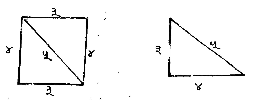
\includegraphics[scale=0.8]{graphics/capture29.png}
     \captionsetup{labelformat=empty}
\vspace{-2mm}
\caption{आयतक्षेत्रदर्शनम्\hspace{2cm} जात्यत्र्यस्रदर्शनम्~।\hspace{-0.8cm} }
\end{figure}

 एतत्कर्णपथाद्विदलितं जात्यम्~। 
\vspace{2mm}

 जातः कर्णः ५~। कर्णभुजाभ्यां जाता कोटिः ४~। श्रुतिकोटिभ्यां जातो बाहुः ३~। \\

 \textbf{सूत्रम्~।} 
\begin{quote}
    \bs
मूलग्रहणेऽप्राप्ते \\
यो राशिरमूलदः करण्याख्यः~।\\
\footnote{'{\color{violet}वर्गेण वर्गं गुणयेद्भजेद्वा}'\textendash\ इति {\color{violet}भास्करबीजगणितो}दितानुरूपम्~। }सङ्गुणनं भजनं वा \\
कुर्याद्वर्गस्य वर्गेण~॥~२८~॥\\
 \footnote{'{\color{violet}लघ्व्या हृतायास्तु पदम्}' इति {\color{violet}भास्करबीजगणितो}दितानुरूपम्~। }लघुहृतबृहत्करण्याः \\
पदं सरूपं विरूपकं स्वघ्नम्~।\\
लघ्वाहतं करण्योः \\
योगवियोगौ करण्यौ स्तः~॥~२९~॥
\end{quote}

\newpage%%%%%%%%%%%%%%%%%%%%%%%%%%%%%%%%%%%%%%%%%%%%

\begin{quote}
    \bs
यदि न पदं च करण्योः \\
पृथक् स्थितिः स्यात् स्वमृणमेवम्~।
\end{quote}

\setcounter{footnote}{0}
\textbf{ अथ करण्या आसन्नमूलानयने सूत्रम्~। }

\phantomsection \label{4.31}
\begin{quote}
    \bs 
     \footnote{'{\color{violet}वर्गेण महतेष्टेन}' इत्यादि {\color{violet}भास्करलीलावत्यु}दितानुरूपम्~। }हरहतकरणीराशेः \\
     शतादिवर्गेण केनचिन्महता~॥~३०~॥\\
गुणितान्मूलं गुणपद-\\
हरहतिभक्तं पदं निकटम्~। 
\end{quote}

 \textbf{उदाहरणम्~।} 
\begin{quote}
    \bqt 
     समचतुरस्रे षट्कर-\\
     बाहूनि विद्वन् वदाशु मे कर्णम्\footnote{The reading कर्णं मे doesn't fit in meter.}।\\
सत्र्यंशत्रिकपञ्चक-\\
कोटिभुजेऽप्यायते कथय~॥~२५~॥
\end{quote}

 न्यासः~। 
\vspace{-2mm}

\begin{figure}[h!]
    \centering
    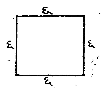
\includegraphics[scale=0.8]{graphics/capture30.png}
\end{figure}
\vspace{-2mm}

 अत्र कोटिबाहुकृतियुतिः ७२~। अस्य मूलग्रहणेऽप्राप्तेऽमूलदत्वाज्जाता करणी ७२ इयं '\hyperref[4.31]{शतादिवर्गेण}'\textendash\ इति शतवर्गेण गुणिता 

\newpage%%%%%%%%%%%%%%%%%%%%%%%%%%%%%%%%%%%%%%%%%%%%
\noindent ७२०००० मूलम् ८४८~। अहरत्वाद्रूपहरघ्नशतेन भक्तं जातः 
$\mbox{८}\frac{\mbox{१२}}{\mbox{२५}}$~। \\

\vspace{-4mm}
दर्शनम्
\begin{figure}[h!]
    \centering
    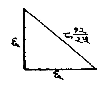
\includegraphics[scale=0.85]{graphics/capture31.png}
\end{figure}

आदिशब्दात्\; सहस्रायुतादि । सहस्रवर्गेण\; गुणिते जातः कर्णः\; $\mbox{८}\frac{\mbox{९७}}{\mbox{२००}}$~। अयुतवर्गे गुणके कृते जातः कर्णः $\mbox{८}\frac{\mbox{२१३}}{\mbox{२५००}}$~। यावद्यावन्महति गुणके कृते तावत् तावदासन्नपदं भवति~।\\

\vspace{-2mm}
 अथ द्वितीयोदाहरणस्य न्यासः । अत्र जाता वर्गकरणी $\dfrac{\mbox{३५६}}{\mbox{९}}$ ।
\begin{figure}[h!]
    \centering
    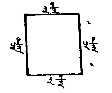
\includegraphics[scale=0.85]{graphics/capture32.png}
\end{figure}

\noindent अस्मिन् राशौ छेदस्थितैर्नवभिः करणीत्वाच्छतवर्गेण च गुणितो
जातः ३२०४००००~। अस्मान्मूलम् ५६६० एतद्गुणपदं १०० हरश्च ९ अनयोराहत्या
९०० भक्तं जातः कर्णः $\mbox{६}\frac{\mbox{१३}}{\mbox{४५}}$~। \\

\vspace{-4mm}
दर्शनम्
\begin{figure}[h!]
    \centering
    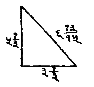
\includegraphics[scale=0.85]{graphics/capture33.png}
\end{figure}
\newpage
%%%%%%%%%%%%%%%%%%%%%%%%%%%%%

 \textbf{सूत्रम्~।} 
\begin{quote}
    \bs
    भुजकोटिश्रवणानां \\
    द्वन्द्वसमासेऽन्तरेऽथवा जातम्~॥~३१~॥\\
सङ्क्रमसूत्रैरुह्यं \\
तत्तत्करणं स्वयं बुद्ध्या~। 
\end{quote}

 \textbf{कोटिकर्णयुतौ भुजे च दृष्ट उदाहरणम्~।} 
\begin{quote}
    \bqt 
    षड्वर्गहस्तप्रमितश्च वंशः \\
    तस्यैकदेशः पवनेन भग्नः~।\\
लग्नोऽत्र मूलान्तरभूर्गजघ्न-\\
त्रिसङ्ख्यहस्ता\footnote{The reading -हस्ते seems to be a typographical error.} वद वंशखण्डे~॥~२६~॥
\end{quote}
 
 न्यासः~। \\

\vspace{-4mm}
 अत्र कोटिकर्णयोगः ३६~। वंशाग्रमूलान्तरं भुजः २४~। अस्य
वर्गः ५७६ एतत् कोटिकर्णवर्गान्तरम्~। अथ योगहृतमित्यन्तरम्
१६~। योगो द्विष्ठ इति सङ्क्रमणेन जाते वंशस्योर्ध्वाधरे खण्डे
श्रुतिकोटिरूपे २६~। १०~। \\

\vspace{-4mm}
दर्शनम्~। 

\begin{figure}[h!]
    \centering
    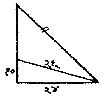
\includegraphics[scale=0.8]{graphics/capture34.png}
\end{figure}
\newpage
%%%%%%%%%%%%%%%%%%%%%%%%%%%%%%%%%%%%%%%%%%%%
 
 \textbf{भुजकर्णयोगे कोटौ च दृष्टम् उदाहरणम्~।} 
\begin{quote}
\bqt
 युद्धे हस्तचतुर्दशोच्छ्रय इभः \\
 तस्मान्नगघ्नान्तरे \\
 धानुष्कोऽमुचदाशुगं करिकर-\\
 च्छित्यै भटेनामुना~।\\
मुक्तेनाशु निजाशुगेन तदिषुः \\
छिन्नस्तयोर्बाणयोः \\
संयोगात् कतिभिः करैः स्थित इभः \\
तुल्याध्वनोस्तद्वद~॥~२७~॥
\end{quote}
 
 अत्र धानुष्कगजान्तरं भुजकर्णयोगः ९८~। ज्ञातो गजशुण्डोच्छ्रयः कोटिः १४, अस्य वर्गो भुजकर्णवर्गान्तरम् १९६~। एतद्भुजकर्णयोगेन ९८ हृतं जातमन्तरम् २~। योगो द्विष्ठ इति सङ्क्रमणेन जातौ क्रमेण भुजकर्णौ ४८~। ५० एते शरगतिशरयोगगजान्तरे~। \\
 
\vspace{-4mm}
क्षेत्रदर्शनम्~। 

\begin{figure}[h!]
    \centering
    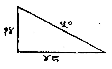
\includegraphics[scale=0.85]{graphics/capture35.png}
\end{figure}

 \textbf{अथ कोटिकर्णान्तरे भुजे च दृष्टम् उदाहरणम्~।} 
 \begin{quote}
     \bqt 
 कासारे घनसारसावलिरसा-\\
 रेङ्खत्सरे सारसं
 \end{quote}
\newpage
%%%%%%%%%%%%%%%%%%%%%%%%%%%%%%%%%%%%%%%%%%%%%%%%%%%%%
 \begin{quote}
     \bqt 
 राजीवस्थिरजीववन्मुकुलितं \\
 हस्तैकमात्रोच्छ्रितम्~।\\
सप्तस्वेव करेषु मन्थरमरुत्-\\
सञ्चारसञ्चालनैः \\
मग्नं तज्जलनिम्नतां कथय मे \\
राजीवनालोच्छ्रितिम्~॥~२८~॥
 \end{quote}

 न्यासः~। 
\begin{figure}[h!]
    \centering
    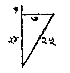
\includegraphics[scale=0.85]{graphics/capture36.png}
\end{figure}

 अत्र नालान्मग्नस्थानं भुजः ७ अस्य वर्गः कोटिकर्णवर्गान्तरम्
४९~। जलोपरिस्थितकमलकलिकारूपेण कोटिकर्णान्तरेण १ भक्तं
जातो योगः ४९~। योगो द्विष्ठ इति जातौ कोटिकर्णौ २४~। २५~। \\
\indent अत्र कोटिर्जलगाम्भीर्यम्~। कर्णो नालमानमेवं भुजकोटिकर्णाः~। \\

\vspace{-2mm}
\setcounter{footnote}{0}
 \textbf{सूत्रम्~।} 
\begin{quote}
    \bs
    \footnote{अस्योपपत्तिरग्रिमपृष्ठे विलोक्या~। }कर्णाश्रितभुजवर्गा-\\
    न्तरसंयुतकर्णवर्गसम्भक्तः~॥~३२~॥\\
श्रुतिकृतिहतगम्यभुजः \\
तुल्योऽध्वा\footnote{The reading भुजतुल्योऽध्वा doesn't give correct meaning as well as doesn't fit in meter.} कोकयोर्योगे~।
\end{quote}
\newpage%%%%%%%%%%%%%%%%%%%%%%%%%%%%%%%%%%%%%%%%%%%%
 \textbf{उदाहरणम्~।} 
\begin{quote}
    \bqt 
     षोडशहस्तायामा \\
     याम्योत्तरयोश्च पूर्वपश्चिमयोः~।\\
द्वादशकरविस्तारा \\
वापी रथचार-दम्पती रात्रौ~॥~२९~॥
\end{quote}
\blfootnote{\hspace{-4mm} आ का गा घा चतुर्भुजे आ घा $= \mbox{भु}_{\text{१}}$~। घा गा $= \mbox{भु}_{\text{२}}$~। 
आ गा $=$ कर्णमानम् $=$ क~। आ स्थाने कोकः~। गा स्थाने कोकी,
\begin{center}
    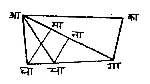
\includegraphics[scale=0.8]{graphics/capture37.png}
\end{center}
प्रातःकाले कोकी गा घा भुजे चलिता, इति कल्प्यते~। घा स्थानात् 
आ गा कर्णोपरि घा मा लम्बः~। चा स्थाने च द्वयोर्युतिस्तदा
गा चा $=$ आ चा $=$ समगतिः~। चा स्थानात् कर्णोपरि लम्बः $=$
चाना~। गाना $=$ आना $= \dfrac{\mbox{क}}{\mbox{२}}$~। आ घा गा त्रिभुजे मा गा $=$ 
\vspace{2mm}

\hspace{15mm} $\dfrac{\mbox{क}^{\text{२}} + (\mbox{भु}^{\text{२}}_{\text{२}} - \mbox{भु}^{\text{२}}_{\text{१}})}{\mbox{२\,क}}$~।~ ततस्त्रिभुजयोः साजात्यात्
\vspace{2mm}

\hspace{4mm} गा चा $= \dfrac{\mbox{घा गा} \times \mbox{गा ना}}{\mbox{मा गा}} = \dfrac{\dfrac{\mbox{क}}{\mbox{२}} \times \mbox{भु}^{\text{२}}}{\dfrac{\mbox{क}^{\text{२}}  +
(\mbox{भु}^{\text{२}}_{\text{२}} -\mbox{भु}^{\text{२}}_{\text{१}})}{\mbox{२\,क}}} = \dfrac{\mbox{क}^{\text{२}} \times \mbox{भु}_{\text{२}}}{\mbox{क}^{\text{२}} +(\mbox{भु}^{\text{२}}_{\text{२}} - \mbox{भु}^{\text{२}}_{\text{१}})}$~~ इत्युपपन्नम्~। 
}
\newpage%%%%%%%%%%%%%%%%%%%%%%%%%%%%%%%%%%%%%%%%%%%%
\begin{quote}
    \bqt 
     विश्लिष्टौ प्रागुत्तर-\\
     कोणे कोकः स्थितः कोकी~।\\
याम्योत्तरे प्रगे सा \\
याम्यभुजेनोद्यता गन्तुम्~॥~३०~॥\\
दृष्ट्वा तां कर्णपथात् कोको \\
द्रुतमेत्य रतिमना मिलितः~।\\
समगतिमानं च तयोर्वद \\
यदि गणितं विजानासि~॥~३१~॥
\end{quote}

 न्यासः~। 
\vspace{-2mm}

\begin{figure}[h!]
    \centering
    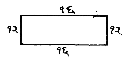
\includegraphics[scale=0.8]{graphics/capture38.png}
\end{figure}
\vspace{-3mm}

 प्राग्वत् कर्णः २०~। जाता चक्रवाकदम्पत्योः समगतिः $\mbox{१२}\frac{\mbox{१}}{\mbox{२}}$~। एवं
विषमचतुरस्रेऽपि~। \\

\phantomsection \label{4.33}
\setcounter{footnote}{0}
 \textbf{सूत्रम्~।} 
\begin{quote}
    \bs 
 \footnote{'{\color{violet}सर्वदोर्युतिदलं चतुःस्थितम्}' इत्यादि {\color{violet}भास्करो}क्तानुरूपमेवेदम्~। }भुजयोगदलं चतुःस्थितम् \\
 ऊनं दोर्भिश्च तद्वधान्मूलम्~॥~३३~॥
\end{quote}

\newpage%%%%%%%%%%%%%%%%%%%%%%%%%%%%%%%%%%%%%%%%%%%%

\begin{quote}
    \bs 
 त्र्यस्रे तु स्फुटगणितं \\
 चतुरस्रे क्वचिदस्फुटं स्यात्\footnote{The reading भवति doesn't fit in meter.}।
\end{quote}

 \textbf{उदाहरणम्~।} 
\begin{quote}
    \bqt 
     स्थूलविधावुक्तानां \\
     समचतुरस्रायतादिकानां मे~।\\
त्र्यस्राणामपि गणितं \\
सूक्ष्मं गणितज्ञ कथयाशु~॥~३२~॥
\end{quote}

 न्यासः~। 
\begin{figure}[h!]
    \centering
    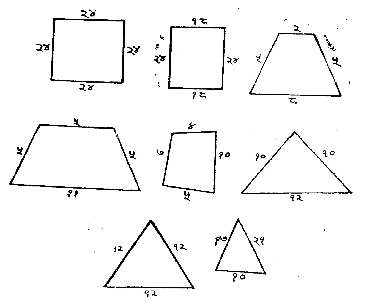
\includegraphics[scale=0.8]{graphics/capture39.png}
\end{figure}
\newpage
%%%%%%%%%%%%%%%%%%%%%%%%%%%%%%%%%%%%%%%%%%%
 पञ्चानां चतुरस्राणां सूक्ष्मफलानि ४००~। ४३२~। २०~। ३२~। ३६ समत्रिभुजस्य सूक्ष्मफलं करणी ३८८८~। द्विसमविषमयोः फले ४८~। ८४
अनयोस्त्र्यस्रयोः स्फुटमेव भवति~। चतुरस्रस्य क्वचिन्न भवति~। 
अतः {\color{violet}श्रीधराचार्येण} '{\color{violet}भुजयुतिदलं चतुर्धा}'\textendash\ इत्युक्तं तद्यथा\textendash\\

\vspace{-2mm}
 \textbf{उदाहरणम्~।} 
\begin{quote}
    \bqt 
     भूरेकविंशतिर्यत्र \\
 दशसप्तदशोन्मितौ~। \\
 बाहू द्वादश वक्त्रं च \\
 लम्बोऽष्टौ तत्र किं फलम्~॥~३३~॥~
\end{quote}

 न्यासः~।  \\
 
 \vspace{-3mm}
क्षेत्रम्~।
 \vspace{-2mm}
\begin{figure}[h!]
    \centering
    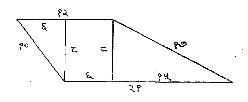
\includegraphics[scale=0.8]{graphics/capture40.png}
\end{figure}
 \vspace{-2mm}
 
 अथ भुजयोगदलमित्यादिना जाता फलकरणी ४२१२०~। \\
 
 \vspace{-3mm}
 अत्र '\hyperref[4.34.1]{समलम्बे भूमुखयुतिदलहतलम्बफलं चतुर्बाहौ}' इति वक्ष्यमाणसूत्रेण सूक्ष्मफलम् १३२~। अस्य वर्गः फलकरणी १७४२४
इयं पूर्वकरण्या सदृशी न स्यात्~। तस्मात् फले विसंवादः~। तयोः 
फलयोरेतदेव १३२ ग्राह्यम्~। अन्यत्र ग्राह्यमनुपपन्नत्वात्~। \\

\vspace{-3mm}
 उपपत्तयेऽस्य क्षेत्रस्य खण्डत्रयं कृत्वा पृथक् पृथक् फलान्यानीयैकत्र संयोज्य फलो-पपत्तिर्दर्शनीया~। 
\newpage
%%%%%%%%%%%%%%%%%%%%%%%%%%%%%%%%%%%%%%%%%%%%%%%%

 तद्यथा~। '\hyperref[4.38]{लम्बकृतिबाहुवर्गान्तरतो मूलं तदाबाधा}' इति
वक्ष्यमाणसूत्रेण लम्बभुजौ ८~। १७ अनयोः कृती ६४~। २८९ अनयोरन्तरम् २२५ अस्य मूलमाबाधा १५~। एतन्मित-भुजलम्बाभ्यामाभ्यां
१०~। ८ जाताबाधा ६~। \\

\vspace{-3mm}
अथ क्षेत्रदर्शनम्~।
\vspace{-2mm}
\begin{figure}[h!]
    \centering
    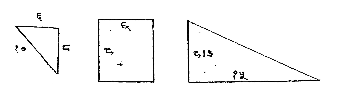
\includegraphics[scale=0.8]{graphics/capture41.png}
\end{figure}
 \vspace{-2mm}

 भुजमित्यादिना खण्डत्रयफलानि २४~। ४८~। ६०~। एषामैक्यं सर्वक्षेत्रफलम् १३२~। \\

\vspace{-2mm}
\setcounter{footnote}{0}
 \textbf{सूत्रम्~।} 
\phantomsection \label{4.34.1}
\begin{quote}
    \bs 
    \footnote{'{\color{violet}लम्बेन निघ्नं कुमुखैक्यखण्डम्}' इत्यादि {\color{violet}भास्करो}क्तमेतदनुरूपमेव~।}समलम्बे भूमुखयुति-\\
    दलहतलम्बं फलं चतुर्बाहौ~॥~३४~॥
\end{quote}
 
 \textbf{उदाहरणम्~।} 
\begin{quote}
    \bqt 
     क्षेत्रस्य यस्य वदनं निधयो धरित्र्यां \\
     रूपाश्विनो भुजयुगे वियदिन्दवश्च~।
\end{quote}

\newpage
%%%%%%%%%%%%%%%%%%%%%%%%%%%%%%%%%%%%%%
\begin{quote}
    \bqt 
 लम्बोऽपि कुञ्जरमितो वद तस्य विद्वन् \\
 सूक्ष्मं फलं यदि\footnote{The reading वद seems to be a redundancy error and doesn't give a correct meaning.} तवास्त्यभिमानलेशः~॥~३४~॥
\end{quote}

 न्यासः~। 
 \vspace{-2mm}
\begin{figure}[h!]
    \centering
    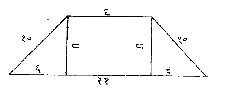
\includegraphics[scale=0.8]{graphics/capture42.png}
\end{figure}
 \vspace{-2mm}

 जातं सूक्ष्मफलम् १२०~। \\

\vspace{-2mm}
 \textbf{अपि च~।} 
\begin{quote}
    \bqt
     त्र्यस्रस्य यस्य लम्बोऽष्टौ \\
     दशसप्तदशोन्मितौ~।\\
बाहू भूरेकविंशत्या \\
सम्मिता मे फलं वद~॥~३५~॥
\end{quote}

 न्यासः~। 
\vspace{-2mm}
\begin{figure}[h!]
    \centering
    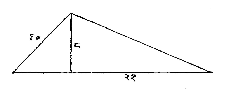
\includegraphics[scale=0.8]{graphics/capture43.png}
\end{figure}
\vspace{-2mm}

 सूक्ष्मफलम् ८४~। 
\newpage
%%%%%%%%%%%%%%%%%%%%%%%%%%
\setcounter{footnote}{0}
 \textbf{सूत्रम्~।} 
\begin{quote}
    \bs 
     \footnote{आचार्येण ५०० व्यासे १५८१ परिधिः सूक्ष्मोऽप्यङ्गीकृतः~। 
अतोऽत्र सूक्ष्मपरिधिः 
\begin{equation*}
     = \dfrac{\mbox{१५८१ व्या}}{\mbox{५००}} = \dfrac{\mbox{५२७} \times \mbox{३ व्या}}{\mbox{५००}} = \dfrac{\mbox{५२७} \times \mbox{स्थू प}}{\mbox{५००}}
\end{equation*}

\hspace{2mm} एवमन्यत्रापि~। अतः उपपन्नम्~। परिध्यानयनं भास्करस्यैव
सूक्ष्मम् (\,द्रष्टव्या भास्करलीलावत्यां पूज्य-पादपितृटिप्पणी\,)~। }स्थूलं वृत्तादौ यत् \\
भशरघ्नं तत्खखेषुहृत् सूक्ष्मम्~।\\
त्र्यादिषु च मण्डलेष्वपि \\
रश्मिषु च चतुस्त्रिबाहुमृते~॥~३६~॥
\end{quote}

 \textbf{उदाहरणम्~।} 
\begin{quote}
    \bqt 
     स्थूलविधावुक्तानां \\
     समवर्तुलशङ्खचापानाम्~।\\
हीरकरदनेम्यर्भकशशि-\\
यवढक्कामृदङ्गचक्राणाम्~॥~३५~॥ 
\vspace{2mm}

 पञ्चास्रषडस्रकयोः \\
 त्र्यादीनां मण्डलानां च~।
\end{quote}

\newpage%%%%%%%%%%%%%%%%%%%%%%%%%%%%%%%%%%%%%%%%%%%%
\begin{quote}
    \bqt 
वद गणितं मे सूक्ष्मं \\
विद्वन् गणितं प्रवेत्सि यदि~॥~३७~॥ 
\end{quote}

स्थूलोदितसमवृत्तपरिधिफले ३०।७५ अतः सूक्ष्मपरिधिफले $\mbox{३१}\frac{\mbox{३१}}{\mbox{५०}}$~। 
$\mbox{७९}\frac{\mbox{९}}{\mbox{२०}}$~। शङ्खस्य परिधिफले ६०।१३२ अतः
सूक्ष्मे $\mbox{६३}\frac{\mbox{६}}{\mbox{२५}}$~। 
$\mbox{३२८}\frac{\mbox{१०६}}{\mbox{१२५}}$~। चापयोः स्थूले सूक्ष्मकाष्ठे $\mbox{१४}\frac{\mbox{३७८}}{\mbox{५००}}$~। $\mbox{२९}\frac{\mbox{६४}}{\mbox{५००}}$~। गजदन्तनेमिबालेन्दुयववज्रढक्कामृदङ्गचक्राणां स्थूलफलानि ३५।२४।२७।१८।३२।४०।८०।६०। जातानि सूक्ष्मफलानि $\mbox{३६}\frac{\mbox{८९}}{\mbox{१००}}$~। $\mbox{२५}\frac{\mbox{३७}}{\mbox{१२५}}$~। $\mbox{२८}\frac{\mbox{२२९}}{\mbox{५००}}$~। $\mbox{१८}\frac{\mbox{१८}}{\mbox{२५}}$~।
$\mbox{३३}\frac{\mbox{९१}}{\mbox{१२५}}$~। $\mbox{४२}\frac{\mbox{४}}{\mbox{२५}}$~। $\mbox{८४}\frac{\mbox{८}}{\mbox{२५}}$~। $\mbox{६३}\frac{\mbox{६}}{\mbox{२५}}$~।
पञ्चास्रषडस्रयोः स्थूले फले ६०।९०~। जाते सूक्ष्मे $\mbox{६३}\frac{\mbox{६}}{\mbox{२५}}$~। $\mbox{९४}\frac{\mbox{४३}}{\mbox{५०}}$~।
त्र्यस्रादीनां मण्डलफलानि २४।४८।८०।१२०~। सूक्ष्माणि जातानि $\mbox{२५}\frac{\mbox{३७}}{\mbox{१२५}}$~।
$\mbox{५०}\frac{\mbox{७४}}{\mbox{१२५}}$~। $\mbox{८४}\frac{\mbox{८}}{\mbox{२५}}$~। $\mbox{१२६}\frac{\mbox{१२}}{\mbox{१५}}$~। एवं वृत्तरेखाश्रितानि यानि क्षेत्राणि तेषां स्वकरणेन स्थूलफलान्यानीय
तेभ्यः सूक्ष्मफलानि ज्ञेयानि~।\\

\setcounter{footnote}{0}
 \textbf{सूत्रम्~।} 
\begin{quote}
    \bs 
 \footnote{'{\color{violet}त्रिभुजे भुजयोर्योगस्तदन्तरहृतः~।}' इत्यादि {\color{violet}भास्करो}दितानुरूपमेवेदं सर्वम्~।}त्र्यस्रे भुजयोः संयुति-\\
 वियुतिवधो भूविभाजितो\footnote{The reading भूविभाजिता seems to be a typographical error.} लब्ध्या~। 
\end{quote}

\newpage%%%%%%%%%%%%%%%%%%%%%%%%%%%%%%%%%%%%%%%%%%%%
\phantomsection \label{4.36}
\begin{quote}
    \bs 
द्विष्ठा भूमी रहिता \\
सहिता दलिता तदाबाधे~॥~३६~॥ 
\vspace{1mm}

अल्पानल्पाबाधे \\
क्रमशस्ते सन्धिपीठसञ्ज्ञे तु~।\\
लम्बनिपातादल्पा-\\
नल्पभुजदिगाश्रिते भवतः~॥~३७~॥ 
\vspace{1mm}

\phantomsection \label{4.38}
भुजवर्गात् स्वाबाधा-\\
वर्गविहीनात् पदं लम्बः~।\\
लम्बकृतिबाहुवर्गा-\\
न्तरतो मूलं तदाबाधा~॥~३८~॥
\vspace{1mm}

\phantomsection \label{4.39}
अवलम्बाबाधाकृति-\\
योगान्मूलं तु तद्बाहुः~।\\
लम्बाहतमवनिदलं \\
त्रिभुजे गणितं स्फुटं भवति~॥~३९~॥
\end{quote}

 \textbf{उदाहरणम्~।} 
\begin{quote}
    \bqt 
बाहू त्रिपञ्चप्रमितौ दशाढ्यौ \\
भूः शक्रतुल्या त्रिभुजस्य यस्य~।
\end{quote}
\newpage
%%%%%%%%%%%%%%%%%%%%%%%%%%%%%%%%%%%%%%%%%%%%%%%%%%%%

\begin{quote}
    \bqt 
तस्याबधे लम्बमिती प्रचक्ष्व \\
सूक्ष्मं फलं चाशु यदि प्रवेत्सि~॥~३८~॥
\end{quote}

 न्यासः~। 
 \vspace{-2mm}
 
\begin{figure}[h!]
    \centering
    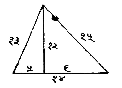
\includegraphics[scale=0.8]{graphics/capture44.png}
\end{figure}
 \vspace{-2mm}

 जाते अबाधे ९।५ अनयोरेकस्याल्पस्य ५ सन्धिसञ्ज्ञा~। अनल्पस्य पीठसञ्ज्ञा ९~। जातो लम्बः १२~। गणितम् ८४~। \\

\vspace{-2mm}
 \textbf{अपि च~।} 
\begin{quote}
    \bqt 
     नखविश्वोन्मितौ बाहू \\
     मही रुद्रमिता सखे~।\\
यत्र त्र्यस्रे वदाबाधे \\
लम्बं सूक्ष्मं फलं\footnote{The reading वद seems to be a redundancy error and doesn't give a correct meaning.} द्रुतम्~॥~३९~॥ \\
 भुजौ लम्बाबधाभ्यां च \\
 लम्बदोर्भ्यां कुखण्डके~। 
\end{quote}

 न्यासः~। \\

\vspace{-2mm}
 अत्र भुजयोः संयुतिः ३३~। वियुतिश्च ७~। अनयोर्घातः २३१~। 
भूविभाजिता लब्धिः २१~। अनया '\hyperref[4.36]{भूमी रहिता}' इति विपरीतशोधनेन विशोध्य जाताल्पाबाधा ऋणम् ५~। महती धनम् १६~। 
अत्र '\hyperref[4.38]{भुजवर्गात् स्वाबाधा}'\textendash\, इत्यल्पाबाधाया ऋणगतायाः ५
\newpage
%%%%%%%%%%%%%%%%%%%%%%%%%%%%%%%%%%%%%%%%%%%
\setcounter{footnote}{0}

\noindent '\hyperref[4.7]{ऋणधनयोश्च कृतिः स्वम्}' इति ऋणगताबाधावर्गो धनम् २५~। 
भुजवर्गादस्मात् १६९ अपास्य शेषं १४४~। अस्य मूलं लम्बः १२~। 
अथ लम्बवर्गं भुजवर्गादपास्य शेषम् २५~। अस्य मूलम् ५~। 'स्वमूलं धनर्णं वा'\textendash\ इति ऋणम् ५ यतः क्षेत्रान्तर्वर्तिलम्बो न भवति~। \\

\vspace{-3mm}
 तथा क्षेत्रदर्शनम्~। 
\vspace{-2mm}

\begin{figure}[h!]
    \centering
    % \captionsetup{labelformat=empty}
    %\caption{\bt अथ क्षेत्रदर्शनम्~।}
    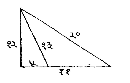
\includegraphics[scale=0.85]{graphics/capture45.png}
\end{figure}
\vspace{-2mm}

 अत्र '\hyperref[4.39]{लम्बाहतमवनिदलम्}'\textendash\ इति क्षेत्रफलम् ६६~। \\

\setcounter{footnote}{0}
\textbf{ अथ क्षेत्रलक्षणे सूत्रम्~। }
\begin{quote}
    \bs 
     \footnote{'{\color{violet}धृष्टोद्दिष्टमृजुभुजक्षेत्रे}' इत्यादि {\color{violet}भास्करो}दितानुरूपमेव~।}ऋजुबाहुनि चतुरस्रे \\
     त्र्यस्रे वानल्पबाहुतः स्वल्पम्~।\\
सदृशं वान्यभुजैक्यं \\
यत्र क्षेत्रे तदक्षेत्रम्~॥~४०~॥
\end{quote}

 \textbf{उदाहरणम्~।} 
\begin{quote}
    \bqt 
     दुष्टस्पष्टसमीरिते स्मृतिकरा \\
     धात्री शराङ्कोन्मितौ\footnote{The reading शराङ्गोन्मितौ seems to be an error. \textit{Aṅga} (subsidiary parts of the \textit{Vedas}) is a \textit{bhūta-saṅkhyā} (word numeral) that stands for the number $6$. In the commentary of this verse, the number $9$ is used. In \textit{bhūta-saṅkhyā} system, $9$ is represented by the word \textit{aṅka}.}
\end{quote}
\newpage%%%%%%%%%%%%%%%%%%%%%%%%%%%%%%%%%%%%%%%%%%%%

\begin{quote}
    \bqt 
 बाहू चाननमब्धिसङ्ख्यकम्\\
 ऋजुक्षेत्रे चतुर्बाहुके~।\\
त्र्यस्रे षट्-तिथिदोष्णि धिष्ण्यभुवि भोः \\
क्षेत्रज्ञ चात्रास्ति वा\\
नास्तीत्याशु फलं प्रदर्शय यदि \\
प्रौढोऽसि पाटीविधौ~॥~४०~॥
\end{quote}

 न्यासः~। 
\begin{figure}[h!]
    \centering
    % \captionsetup{labelformat=empty}
    %\caption{\bt अथ क्षेत्रदर्शनम्~।}
    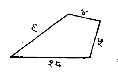
\includegraphics[scale=0.85]{graphics/capture46.png}
\end{figure}

 अत्र फलाभावः~। तावच्चतुरस्रे '\hyperref[4.33]{भुजयोगदलं चतुःस्थित}'मित्यादिना जातं करणीगतगणितम् १८४०~। \\

\vspace{-2mm}
 अत्र {\color{violet}श्रीधराचार्येण} लम्बाबाधाप्त्यै यदुपलक्षणमुक्तं तन्न~। 
तद्यथा\textendash\ 
\begin{quote}
    {\bq 
    पार्श्वभुजान्तरसंयुतिवधो \\
    मुखहीनभूकृतिर्येषाम्~।\\
समलम्बानामधिका \\
तेषां लम्बाबधाप्तिः~॥} इति~।
\end{quote}
 
 पार्श्वभुजयोरन्तरम् ४~। युतिश्च १४~। अनयोर्हतिः ५६~। अस्या
मुखहीनभूकृतिः १९६ अधिका अतोऽत्र लम्बो भाव्यः~। लम्बसत्त्वे

\newpage
%%%%%%%%%%%%%%%%%%%%%%%%%%%%%%%%%%
\noindent फलाभावो न स्यात्~। अत एव तत्सूत्रं वृथा~। त्रिभुजे तु \renewcommand{\thefootnote}{\fnsymbol{footnote}}\footnote[1]{आचार्येणात्र भास्कराचार्यदूषणं वृथैवोक्तमृजुभुजक्षेत्रेण त्रिभुजस्यापि ग्रहणादिति स्फुटमेव गणित-विदाम्~।}भास्कराचार्येण नियमो न कृतः~। तस्यैव दूषणम्~। तथा हि~। 
\vspace{-2mm}

\begin{figure}[h!]
    \centering
    % \captionsetup{labelformat=empty}
    %\caption{\bt अथ क्षेत्रदर्शनम्~।}
    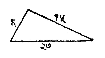
\includegraphics[scale=0.85]{graphics/capture47.png}
\end{figure}
\vspace{-2mm}

\noindent त्रिभुजेऽत्र भुजयोगदलं चतुःस्थितमिति न्यस्तं २४~। २४~। २४~। २४~। विभुजम् १८~। ९~। ३~। २४ एषां घातः ११६६४~। अस्याकृतित्वादृणराशेर्मूलं नास्त्येवेति फलाभाव इति सिद्धम्~।\\

\vspace{-2mm}
 अथात्र {\color{violet}भास्कराचार्य}स्य सूत्रम्~। 
\begin{quote}
    \bq 
    'त्रिभुजे भुजयोर्योगः \\
    तदन्तरगुणो भुवा हृतो लब्ध्या~।\\
द्विष्ठा भूरूनयुता \\
दलिताबाधे तयोः स्याताम्~॥\\
स्वाबाधाभुजकृत्योः\\
अन्तरमूलं प्रजायते लम्बः~।\\
लम्बगुणं भूम्यर्धं \\
स्पष्टं त्रिभुजे फलं भवति~॥'
\end{quote}
\newpage%%%%%%%%%%%%%%%%%%%%%%%%%%%%%%%%%%%%%%%%%%%%

 भुजयोर्योगः २१ अन्तरेण ९ हतः १८९ भुवा २७ हृतो
लब्धम् ७~। अनया द्विष्ठा भूः ऊनयुता दलिता जाते आबाधे १०~। १७
स्वाबाधाभुजकृत्योरन्तरमित्याबाधावर्गौ १००~। २८९ भुजवर्गाभ्यामाभ्यां ३६~। २२५ अन्तरितौ ६४~। ६४ मूलमुभयत्रापि स एव लम्बः
८~। लम्बगुणं भूम्यर्धमिति फलम् १०८~। \\

\vspace{-2mm}
 मन्मतेन '\hyperref[4.38]{भुजवर्गात् स्वाबाधावर्गविहीनात् पदं लम्बः}' इति भुजवर्गौ ३६~। २२५ आभ्यामाबाधावर्गौ १००~। २८९~। अपास्य शेषमृणं
६४ आस्यावर्गत्वान्मूलं नास्तीत्यतः फलाभावः~। 
\begin{figure}[h!]
    \centering
    \captionsetup{labelformat=empty}
    \caption{ चतुर्भुजरेखामात्रं क्षेत्रम्~।\hspace{3cm} त्रिभुजस्य रेखादर्शनम्~।\hspace{-2cm}}
    \vspace{-2mm}
    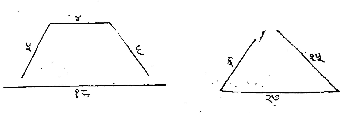
\includegraphics[scale=0.85]{graphics/capture48.png}
\end{figure}
    \vspace{-2mm}
  
 कुगणकपरीक्षणायैव दूषणमुक्तं तदक्षेत्रत्वात्~। \\

 \textbf{सूत्रम्~।}
 \renewcommand{\thefootnote}{\devanagarinumeral{footnote}}
 \setcounter{footnote}{0}
\begin{quote}
\bs 
     \footnote{इदं सर्वं भास्कराचार्येण लीलावत्यामुदितमेव~।}यस्यानियतिश्रुत्योः\\
     चतुरस्रस्य च फले न नियतिः स्यात्~।\\
तेषु भुजेष्वपि कर्णा-\\
वन्यौ बहुधा फलं भवति~॥~४१~॥
\end{quote}
\newpage
%%%%%%%%%%%%%%%%%%%%%%%%%%%%%%%%%%%%%%%%%%%%
\setcounter{footnote}{0}
\begin{quote}
    \bs 
 \footnote{लीलावत्यां भास्करोदितमेव~।}एकं सङ्कोचयता \\
 बाहू कर्णं परं च वर्धयता~।\\
इति कल्पनावशेन \\
स्याच्छ्रुत्योर्ह्रासवृद्धिश्च~॥~४२~॥
\vspace{1mm}

कर्णमभीष्टं प्रथमं \\
परिकल्प्य तदुभयतोऽपि ये त्र्यस्रे~।\\
कर्णो मही तयोर्भुज-\\
भुवौ भुजास्ये भुजौ स्याताम्~॥~४३~॥
\vspace{1mm}

पृथगथ लम्बावबधे \\
लम्बनिपातात् तदेकदिक्स्थितयोः~।\\
आबाधयोश्च विवरात् \\
स्वघ्नाल्लम्बैक्यवर्गसंयुक्तात्~॥~४४~॥ 
\vspace{1mm}

\phantomsection \label{4.45}
मूलं प्रथमः कर्णः \\
श्रुतिदलहतलम्बसंयुतिर्गणितम्~।\\
समचतुरस्रायतयोः\\
भुजकोटिवधः फलं समश्रवसोः~॥~४५~॥
\end{quote}
\newpage%%%%%%%%%%%%%%%%%%%%%%%%%%%%%%%%%%%%%%%%%%%%
 \textbf{उदाहरणम्~।} 
\begin{quote}
    \bqt 
    समचतुरस्रे पञ्चाधिक-\\
    षष्टिभुजे श्रुतिं फलं कथय~।\\
आयतचतुरस्रेऽपि च \\
त्रिचतुर्गुणतत्त्वकोटिभुजे~॥~४१~॥
\end{quote}

 न्यासः~। \\

\vspace{-4mm}
 अत्र भुजकोटिवर्गयुतेर्मूलं कर्णः\textendash\ इति जातः करणीगतः कर्णः
८४५०~। अयं प्रथमः कर्णः कल्पितः~। (\ द्वितीयकर्णज्ञाने एवं\ )
\vspace{-2mm}

\begin{figure}[h!]
    \centering
    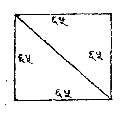
\includegraphics[scale=0.85]{graphics/capture49.png}
\end{figure}
\vspace{-2mm}

\noindent जाते समचतुरस्रान्तस्त्र्यस्रे दर्शनम्~। अथात्र द्वितीयकर्णज्ञानार्थं भूः कर्णः, इतरौ भुजौ भुजाविति त्र्यस्रे~। 
\vspace{-2mm}

\begin{figure}[h!]
    \centering
    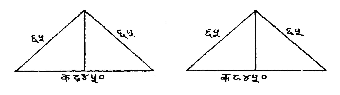
\includegraphics[scale=0.8]{graphics/capture50.png}
\end{figure}
\vspace{-2mm}

 त्र्यस्रयोर्जाते आबाधे समे एव $\dfrac{\mbox{क\,४२२५}}{\mbox{२}},\;\dfrac{\mbox{क\,४२२५}}{\mbox{२}}$\,। लम्बश्च करणीगतः $\dfrac{\mbox{क\,४२२५}}{\mbox{२}}$\,। अत्र लम्बनिपातान्तरम् ० वर्गः ० लम्बै-
\newpage
%%%%%%%%%%%%%%%%%%%%%%%%%%%%%%%%%%%%%%%%%%%%%%%%%%%
\noindent क्यवर्गयुतः ८४५० अस्य मूलं द्वितीयः कर्णोऽमूलदत्वात्
करणीगतः ८४५०~। 

\begin{figure}[h!]
    \centering
   \captionsetup{labelformat=empty}
    \caption{क्षेत्रदर्शनम्~।}
\vspace{-2mm}
    \includegraphics[scale=0.8]{graphics/capture51.png}
\end{figure}
\vspace{-2mm}

 एवं जातौ कर्णौ क ८४५० क ८४५०~। अथ '\hyperref[4.45]{समचतुरस्रायतयोर्भुजकोटिवधः फलम्}' इति जातं समश्रुतौ फलम् ४२२५~। \\
\indent अथवात्र समचतुर्भुजक्षेत्रेऽष्टसप्ततिमितः कर्णः कल्पितः~। \\
\indent अतो जातो द्वितीयः कर्णः १०४~। फलम् ४०५६~। \\
\indent अथवा षट्षष्टिमितः कल्पित एकः कर्णः~। अतो जातो द्वितीयः 
कर्णः ११२~। फलम् ३६९६~। \\
\indent अथ वैकपञ्चाशन्मितः कर्णः कल्पितोऽतो द्वितीयः कर्णः १२०~। 
फलम् ३०००~। \\
\indent अथवा द्वात्रिंशन्मितः कर्णः कल्पितोऽतो द्वितीयः कर्णः १२६~। 
फलम् २०१६~। \\
\indent एवं प्रथमकर्णो यावद्यावद्ध्रासतां समायाति तावत्तावद्द्वितीयकर्णो वृद्धिम् उपयाति~। अतश्चतुरस्राणां फलनियमो नास्तीति सिद्धम्~। \\
\indent अथ द्वितीयोदाहरणे न्यासः~। 

\begin{figure}[h!]
    \centering
   \captionsetup{labelformat=empty}
    \caption{क्षेत्रदर्शनम्~।}
\vspace{-2mm}
    \includegraphics[scale=0.8]{graphics/capture52.png}
\end{figure}

\newpage
%%%%%%%%%%%%%%%%%%%%%%%%%%%%%5

 अत्र कर्णे क्षितौ कल्पितायां जाते आबाधे ८०~। ४५~। लम्बः ६०~। 
इत्थमुभयत्र~। अत्र लम्बैक्यम् १२०~। अस्य वर्गः १४४००~। लम्बनिपातान्तरवर्गेण १२२५ युतो जातो द्वितीयकर्णवर्गः १५६२५~। अस्य
मूलं द्वितीयः कर्णः १२५~। अयं प्रथमकर्णसमानोऽतो भुजकोटिवधः फलम् ७५००~। \\

\vspace{-3mm}
 अथ वा प्रथमश्रुतिदलम् $\frac{\mbox{१२५}}{\mbox{२}}$
लम्बयोगेन १२० गुणितं जातं
फलं तदेव ७५००~। एवमन्यत्रापि~। \\

\vspace{-2mm}
 \textbf{अपि च~।} 
\begin{quote}
    \bqt 
     दशसप्तदशप्रमितौ \\
     बाहू चतुराहतौ मुखे यस्य~।\\
पञ्चाशदेकयुक्ता \\
पञ्चाढ्या सप्ततिर्मह्याम्~॥~४२~॥
\vspace{1mm}

एकस्मात् परिकल्पित-\\
कर्णादन्यं वद श्रवणम्~।\\
लघुभुजमुखपरिवर्ते\footnote{The reading परिवर्त्रे seems to be a typographical error.} \\
तत्र वदान्यं सखे कर्णम्~॥~४३~॥
\end{quote}

 न्यासः~। \\

\vspace{-4mm}
 अत्र प्राग्वत् सव्यभुजाग्राद्दक्षिणभुजमूलगामी सप्तसप्ततिमितः कर्णः कल्पितः~। अत्र प्राग्वत् क्षितिः कर्णः कल्पितः~।
जाते त्र्यस्रे~। 
\newpage
%%%%%%%%%%%%%%%%%%%%%%%%%%%%%%%%%%%%%%

\begin{figure}[h!]
    \centering
   \captionsetup{labelformat=empty}
    \caption{क्षेत्रदर्शनम्~।}
\vspace{-2mm}

    \includegraphics[scale=0.8]{graphics/capture53.png}
\end{figure}
\vspace{-2mm}

अत्राबाधालम्बनिपातान्तरम् १३~। अस्य वर्गः १६९~। लम्बैक्य\textendash \,८४\textendash \,वर्ग\textendash \,७०५६\textendash \,युतात् ७२२५ मूलं जातो द्वितीयः कर्णः ८५~। प्राग्वत् फलम् ३२३४~। \\

\vspace{-4mm}
 अथ लघुभुजमुखपरिवर्तने कृते जातं क्षेत्रम्~। 
\vspace{-2mm}
 
\begin{figure}[h!]
    \centering
    \includegraphics[scale=0.8]{graphics/capture54.png}
\end{figure}
\vspace{-2mm}

 अत्र क्षेत्रे प्राग्वदाबाधालम्बानां दर्शनम्~। \\
\indent अत्र लम्बयोग एकः कर्णः ८४~। फलं तदेव ३२३४~। \\
\indent अत्र कर्णकल्पने विशेषोऽस्ति तदर्थं सूत्रम्~। 

\setcounter{footnote}{0}
 \begin{quote}
     \bs 
     \footnote{'{\color{violet}कर्णाश्रितस्वल्पभुजैक्यमुर्वी}' इत्यादि {\color{violet}भास्करो}क्तानुरूपमेवेदम्~।}कर्णाश्रितलघुभुजयोः\\
     योगो भूमिर्भुजौ त्र्यस्रे~।\\
लम्बः साध्यस्तस्मात् \\
नाल्पः कर्णो न भूमितो दीर्घः~॥~४६~॥ 
 \end{quote}

\newpage%%%%%%%%%%%%%%%%%%%%%%%%%%%%%%%%%%%%%%%%%%%%

तदेव चतुरस्रम्~। अत्र भुजौ ६८।७५ एतौ भुजौ, कर्णाश्रितलघुभुजौ ४०।५१ अनयोर्योगो भूमितो दीर्घो भूमिः ९१~। लम्बः करणीगतः ३०२४~। अस्माल्लम्बाद्द्वितीयको लघुर्न स्यात्~। आद्यो भूमितो दीर्घो न स्यात्~। तद्यथा~। कल्पितैकोत्तरसहस्रमिता कर्णकरणी १००१~। अस्य प्राग्वज्जाते त्र्यस्रे~। प्राग्वज्जाताबाधा करणी १००१~। द्वितीयाभावाच्चतुरस्रं त्रिभुजत्वमेति~। तद्दर्शनम्~।
\vspace{-2mm}
 
\begin{figure}[h!]
    \centering
    \includegraphics[scale=0.6]{graphics/capture54_1.png}
\end{figure}
\vspace{-2mm}

अत्र स एव कर्णः करणीगतः १००१~। चत्वारिंशदष्टषष्टिश्च लम्बौ~। तयोरैक्यं द्वितीयः कर्णः १०८~।\\
\indent इत्थं चतुर्भुजस्य त्रिभुजत्वे लम्बादल्पो भूमेरधिकः कर्णो न स्यात्~। एतत् पूर्वाचार्यैः संक्षेपेणोक्तं मया तु बालावबोधार्थं विस्तार्य व्यक्तीकृतम्~।

\begin{center}
\textbf{इत्यनियतविधिः~।}
\end{center}

\textbf{ सूत्रम्~।}
\setcounter{footnote}{0}

\begin{quote}
\bs
\footnote{'{\color{violet}कर्णाश्रितभुजघातैक्यमुभयथा}' इत्यादि {\color{violet}ब्रह्मगुप्तो}क्तमेवेदम्~।}उभयश्रवणाश्रितभुज-\\
वधयोगौ तौ परस्परं विहृतौ~।\\
प्रतिभुजभुजवधयोगा-\\
हतौ तु मूले चतुर्भुजे कर्णाै~॥~४७~॥
\end{quote}

\newpage%%%%%%%%%%%%%%%%%%%%%%%%%%%%%%%%%%%%%%%%%%%%
\setcounter{footnote}{0}

\phantomsection \label{4.51}
\begin{quote}
\bs
 सर्वचतुर्बाहूनां \\
 मुखस्य परिवर्तने यदा विहिते~।\\
कर्णस्तदा तृतीयः \\
पर इति कर्णत्रयं भवति~॥~४८~॥
\vspace{1mm}

तुल्यं कर्णत्रितयं \\
समचतुरस्रे तथा त्रिसमदोष्णि~।\\
द्विद्विसमे तु द्विसमे \\
तुल्यौ द्वावसदृशश्चान्यः~॥~४९~॥ 
\vspace{1mm}

कर्णत्रयं समं स्यात् \\
विषमे च चतुर्भुजे नियतम्~।\\
चतुरस्रान्तस्त्रिभुजे \\
कर्णभुजाविह भुजौ मही भूमिः~॥~५०~॥
\vspace{1mm}

त्रिभुजवदबधे लम्बा-\\
वपि साध्यौ सर्वचतुरस्रे~। \\
 \footnote{\vspace{-4mm} \begin{quote}
{\color{violet}त्रिबाहुकबहिर्लग्नवृत्तव्यासदलं किल~। \\
 भुजयोराहतेः खण्डाल्लम्बाप्तेन समं भवेत्~॥ }
 \end{quote}
 
\hspace{3cm} इति संशोधकोक्तमेवदमनुरूपमेव~।}त्रिभुजस्य भुजाभ्यासे \\
लम्बविभक्ते प्रजायते व्यासः~॥~५१~॥
\end{quote}
\newpage%%%%%%%%%%%%%%%%%%%%%%%%%%%%%%%%%%%%%%%%%%%%

\phantomsection \label{4.52}
\begin{quote}
    \bs 
     द्विगुणव्यासविभक्ते \\
     त्रिकर्णघातेऽथवा गणितम्~।\\
त्रिभुजे चतुर्भुजे वा \\
व्यासस्य दलं प्रजायते हृदयम्~॥~५२~॥
\end{quote}

 \textbf{उदाहरणम्~।} 
\begin{quote}
    \bqt 
     प्रागुक्तसमायतयोः \\
     नियतौ कर्णाै च कोविद क्षिप्रम्~।\\
मुखभुजपरिवर्तनेऽपि \\
च वद नियतः\footnote{The reading च नियतः seems to be a typographical error as it doesn't fit in the meter.} कर्णस्तृतीयः कः~॥~४४~॥
\end{quote}

 न्यासः~। \\

\vspace{-4mm}
 जातौ नियतकर्णौ करणीगतौ ८४५०~। ८४५० एतयोरेकस्तृतीयः
कर्णः ८४५०~। एवं जातं कर्णत्रयम्~।
\vspace{-2mm}

\begin{figure}[h!]
    \centering
    \includegraphics[scale=0.8]{graphics/capture55.png}
\end{figure}
\vspace{-2mm}

 अथ चतुरस्रान्तस्त्रिभुज इत्यादिना भुजाश्रिते आबाधे ०~। ० पीठे
६५~। ६५ भुजमुखपरिवर्ते कृतेऽपि तदेव चतुरस्रम्~। एतौ कर्णौ
करणीगतौ ८४५०~। ८४५० एतयोः एकस्तृतीयः कर्णः ८४५०~। इति
\newpage
%%%%%%%%%%%%%%%%%%%%%%%%%%%%%%%%%%%%%%%%%%
\noindent जातं कर्णत्रयम्~। त्रिभुजस्य भुजाभ्यास इति जातो व्यासः करणीगतः ८४५०~। द्विगुण-व्यासविभक्त इति गणितम् ४२२५~। व्यासदलं हृदयम् क ४२२५~। 

\begin{figure}[h!]
    \centering
   \captionsetup{labelformat=empty}
    \caption{द्वितीयक्षेत्रस्य न्यासः~।}
\vspace{-2mm}
    
    \includegraphics[scale=0.8]{graphics/capture56.png}
\end{figure}
\vspace{-2mm}

 जातौ नियतौ कर्णौ १२५~। १२५ भुजाश्रिते आबाधे ०~। ० पीठे
१००~। १०० लम्बौ ७५~। ७५ भुजमुखपरिवर्तने न्यासः~। जातौ कर्णौ
१२५~। १२० एतयोस्तृतीयः १२०~। इति जातं कर्णत्रयम् १२५~। १२५~। 
१२०~। व्यासः १२५~। गणितम् ७५००~। हृदयम् $\frac{\mbox{१२५}}{\mbox{२}}$~। \\

\vspace{-2mm}
 \textbf{अपि च~।} 
\begin{quote}
    \bqt 
     पञ्चकृतिर्यस्य भुजौ \\
     सप्ताधिकदश मही त्रयं वदनम्~।\\
तस्य श्रवणावबधे \\
वद लम्बव्यासहृदयानि~॥~४५~॥
\end{quote}

 न्यासः~। 

\begin{figure}[h!]
    \centering
   \captionsetup{labelformat=empty}
    \caption{क्षेत्रदर्शनम्~।}
\vspace{-2mm}

    \includegraphics[scale=0.85]{graphics/capture57.png}
\end{figure}
\vspace{-2mm}

\newpage
%%%%%%%%%%%%%%%%%%%%%%%%%%%

 जातौ कर्णौ २६~। २६ सन्धी ७~। १० लम्बौ २४~। २४ भुजपरिवर्ते
न्यासः~। जातौ कर्णौ २६~। 
$\frac{\mbox{२५०}}{\mbox{१३}}$ एतयोस्तृतीयः $\frac{\mbox{२५०}}{\mbox{१३}}$~। इति 
कर्णत्रयम् २६~। २६~। $\frac{\mbox{२५०}}{\mbox{१३}}$~। गणितम् २४० हृदयम् 
$\frac{\mbox{३२५}}{\mbox{२४}}$~। \\

 \textbf{अपि च~।} 
\begin{quote}
    \bqt 
     पञ्चकृतिर्बाहुमुखा-\\
     नीला त्रिगुणत्रयोदशप्रमिता~।\\
कर्णावबधे लम्बं \\
व्यासं गणितं च हृत् कथय~॥~४६~॥
\end{quote}

 न्यासः~। 
\vspace{-2mm}

\begin{figure}[h!]
    \centering
    \includegraphics[scale=0.85]{graphics/capture58.png}
\end{figure}
\vspace{-2mm}

 जातौ कर्णौ ४०~। ४० सन्धी ७~। ७ लम्बौ २४~। २४ पीठे ३२~। ३२ 
भुजपरिवर्तने कृतेऽपि न विशेषः~। तत्कर्णयोरेकस्तृतीयः~। इति 
कर्णत्रयम् ४०~। ४०~। ४०~। व्यासः 
$\frac{\mbox{१२५}}{\mbox{३}}$~। गणितम् ७६८~। हृदयम्
$\frac{\mbox{१२५}}{\mbox{६}}$~। 
\newpage
%%%%%%%%%%%%%%%%%%%%%%%%%%%%%%%%%%%%%%
 \textbf{अपि च~।} 
\begin{quote}
    \bqt 
    व्येकचत्वारिंशद्द्वि-\\
    पञ्चाशद्मितभुजौ\footnote{The reading पञ्चाशद्भुजौ seems to be a typographical error as it doesn't fit in the meter.} धरा षष्टिः~।\\
पञ्चकृतिमितं वदनं \\
सर्वभुजा दशगुणाः सखे यत्र~॥~४७~॥\\
तत्रावबधे लम्बौ \\
व्यासं गणितं च हृत् कथय~।
\end{quote}

 न्यासः~। \\

\vspace{-4mm}
 जातौ कर्णौ ५६०~। ६३० प्रथमभुजाश्रितसन्धिः २६४~। पीठम्
३३६~। लम्बः ४४८~। 

\begin{figure}[h!]
    \centering
   \captionsetup{labelformat=empty}
  \caption{अस्य भुजमुखपरिवर्तने न्यासः~।}
\vspace{-2mm}
    \includegraphics[scale=0.85]{graphics/capture59.png}
\end{figure}
\vspace{-2mm}

 जातौ कर्णौ ६३०~। ५६० एतयोस्तृतीयः ६५०~। 
 
\begin{figure}[h!]
    \centering
   \captionsetup{labelformat=empty}
  \caption{द्वितीयभुजपरिवर्तने कृते न्यासः~।}
\vspace{-2mm}
    \includegraphics[scale=0.85]{graphics/capture60.png}
\end{figure}
\vspace{-2mm}

 कर्णौ ६३०~। ६५० व्यासः ६५०~। गणितम् १७६४००~। हृदयम् ३२५~। 
\newpage
%%%%%%%%%%%%%%%%%%%%%%%%%%%%%
 \textbf{अपि च~।} 
\begin{quote}
    \bqt 
     बाहू तु पञ्चत्रिमितौ\footnote{The reading त्रिपञ्चमितौ doesn't fit in meter.} दशाढ्यौ \\
     भूः शक्रतुल्या त्रिभुजस्य यस्य~।\\
लम्बोऽर्कसङ्ख्यो वद वृत्तमानं \\
स्वान्तं च शीघ्रं यदि चेत् प्रवेत्सि~॥~४८~॥
\end{quote}

 न्यासः~। 
\vspace{-2mm}

\begin{figure}[h!]
    \centering
    \includegraphics[scale=0.85]{graphics/capture61.png}
\end{figure}
\vspace{-2mm}

 जातो व्यासः $\frac{\mbox{६५}}{\mbox{४}}$~। हृदयम् 
 $\frac{\mbox{६५}}{\mbox{८}}$~। \\

 \textbf{सूत्रम्~।} 
\setcounter{footnote}{0}
 \begin{quote}
     \bs 
      \footnote{'{\color{violet}समानलम्बस्य चतुर्भुजस्य मुखोनभूमिम्}' इत्यादि {\color{violet}भास्करो}क्तसममेव~।}समलम्बकचतुरस्रे \\
      विमुखा भूर्भूः प्रजायते त्र्यस्रे~।\\
तावेव भुजौ बाहू \\
आबाधे लम्बकः प्राग्वत्~॥~५३~॥\\
समुखाबाधावर्गात्\\
लम्बकृतियुतात् पदं कर्णः~।\\
 \end{quote}
\newpage%%%%%%%%%%%%%%%%%%%%%%%%%%%%%%%%%%%%%%%%%%%%
 \textbf{उदाहरणम्~।} 
\begin{quote}
    \bqt 
द्विसमत्रिसमसमानां \\
प्रागुक्तानां समानलम्बानाम्~।\\
तेषामबधे लम्बं \\
कर्णाै गणितज्ञ कथयाशु~॥~४९~॥
\end{quote}
 
 अत्र समलम्बद्विसमभुजक्षेत्रस्य न्यासः~। \\
\indent अत्र मुखोनभूरिति त्र्यस्रम्~। 
\vspace{-2mm}

\begin{figure}[h!]
    \centering
    \includegraphics[scale=0.85]{graphics/capture62.png}
\end{figure}
\vspace{-2mm}

 आबाधे ७~। ७ लम्बः २४~। समुखाबाधावर्गात् १०० लम्बवर्ग\textendash \,५७६\textendash \,युतात् ६७६ मूलं कर्णः २६~। 
\vspace{-2mm}

\begin{figure}[h!]
    \centering
    \includegraphics[scale=0.85]{graphics/capture63.png}
\end{figure}
\vspace{-2mm}

 समलम्बत्रिसमभुजक्षेत्रस्य न्यासः~। 
\vspace{-2mm}

 \begin{figure}[h!]
    \centering
    \includegraphics[scale=0.85]{graphics/capture64.png}
\end{figure}
\newpage
%%%%%%%%%%%%%%%%%%%%%%%%%%%%%%%%%%%%%%%%%%%%%%%%%%%%%%%%%%

 अत्रापि मुखोनभूरिति जातं त्र्यस्रम्~। आबाधे ७~। ७ लम्बः
२४~। समुखाबाधावर्गात् १०२४ लम्बवर्ग\textendash \,५७६\textendash \,युतात् १६०० मूलं
४० एवं द्वितीयः कर्णः~। \\

\vspace{-2mm}
 समलम्बविषमभुजक्षेत्रस्य न्यासः~। 
\vspace{-2mm}

\begin{figure}[h!]
    \centering
  % \captionsetup{labelformat=empty}
  %\caption{द्वितीयभुजपरिवर्तने कृते न्यासः~।}
    \includegraphics[scale=0.85]{graphics/capture65.png}
\end{figure}
\vspace{-2mm}

 भूरिति त्र्यस्रम्~। आबाधे ६~। ३४४ लम्बश्च करणीगतः
१५२०६४~। अथ समुखलघ्वाबाधा २५६ वर्गात् ६५५३६
करणीगतलम्बयुतात् २१७६०० मूलं कर्ण इत्यस्य मूलालाभात्
करणीगतोऽयम् २१७६००~। एवं समुखबृहदाबाधा ५९४ वर्गात्
३५२८३६ लम्बकरणीयुतात् ५०४९०० मूलं कर्ण इत्यस्य मूलालाभात् करणीयम् ५०४९००~। एवं कर्णकरण्यौ २१७६००~। ५०४९००
अनयोः प्राग्वदासन्नमूलग्रहणेन कर्णौ
$\mbox{४४६}\frac{\mbox{१०}}{\mbox{२५}}$~। 
$\mbox{७१०}\frac{\mbox{१४}}{\mbox{२५}}$~। 
लम्बश्च
$\mbox{३८९}\frac{\mbox{१९}}{\mbox{२०}}$~। \\

\setcounter{footnote}{0}
 \textbf{सूत्रम्~।} 
\begin{quote}
    \bs 
\footnote{भास्कराचार्यलीलावत्यां सूचीक्षेत्रगणितवत् सर्वमिदम्~।}परलम्बनिजश्रवणौ \\
परपीठहृतौ स्वसन्धिसङ्गुणितौ~॥~५४~॥
\end{quote}

\newpage%%%%%%%%%%%%%%%%%%%%%%%%%%%%%%%%%%%%%%%%%%%%

\begin{quote}
    \bs 
निजलम्बश्रवणयुतेः \\
लम्बश्रवणाधरे खण्डे~।
\end{quote}

 \textbf{उदाहरणम्~।} 
 \begin{quote}
     \bqt 
विषमे चतुरस्रे प्राक् \\
उक्ते श्रोत्रावलम्बयोर्योगात्~।\\
अवलम्बश्रुतिखण्डे \\
सूच्या योगादधो लम्बः~॥~५०~॥\\
तद्भूखण्डे च समे \\
सूचीलम्बं च सूचिकाबाधे~।\\
सूचीबाहू वद यदि \\
वेत्सि क्षेत्रक्रियामखिलाम्~॥~५१~॥
 \end{quote}
 
 न्यासः~। \\

\vspace{-4mm}
 पीठम् ५०४ लम्बः ३७८ पुनः पीठं ३३९ सन्धिः २६४ लम्बः
४४८~। अत्र परलम्बनिजश्रवणौ ४४८~। ५६० परपीठेनानेन ३३६
हृतौ $\frac{\mbox{४}}{\mbox{३}}$~। 
$\frac{\mbox{५}}{\mbox{३}}$
स्वसन्धि\textendash \,९६\textendash \,गुणितौ १२८~। १६० जाते प्रथमकर्णलम्बयोर्योगादधरे खण्डे १६०~। १२८~। एवं द्वितीयकर्णलम्बयोर्योगादधरे खण्डे ३३०~। १९८~। \\

 \textbf{सूत्रम्~।} 
\begin{quote}
     \bs 
पीठे निजलम्बहृते \\
पृथक् च तद्योगभाजिते भूमिः~॥~५५~॥
\end{quote}
 
 
\newpage
%%%%%%%%%%%%%%%%%%%%%%%%%%%%%%%5

\begin{quote}
     \bs 
 श्रुत्योर्योगाल्लम्बः \\
 तद्गुणिते ते कुखण्डे स्तः~।
\end{quote}

 अत्र कर्णयोगादधोलम्बज्ञानार्थं कर्णौ ५६०~। ६३० सन्धिपीठे
९५~। ५०४ पुनः सन्धिः २६ पीठम् ३३६~। अत्र पीठे ३३६ निजलम्बाभ्याम् ३३७~। ४४८ भक्ते $\frac{\mbox{४}}{\mbox{३}}$~। $\frac{\mbox{३}}{\mbox{४}}$ अनयोर्योगः $\frac{\mbox{२५}}{\mbox{१२}}$ अनेन भूमिर्भक्ता जातः कर्णादधोलम्बः २८८~। अनेनैते $\frac{\mbox{४}}{\mbox{३}}$~। $\frac{\mbox{३}}{\mbox{४}}$ गुणिते 
जाते भूखण्डे ३८४~। २१६~। \\

 \textbf{सूत्रम्~।} 
\begin{quote}
    \bs 
निजनिजलम्बविभक्तौ \\
सन्धी तौ स्वयुतिभाजितौ भूघ्नौ~॥~५६~॥ \\
सूच्याबाधे स्यातां \\
स्वसन्धिहृतलम्बसङ्गुणावबधा~।\\
सूचीलम्बः स्यादथ \\
सूचीलम्बेन ताडितौ बाहू~॥~५७~॥ \\
निजनिजलम्बविभक्तौ \\
बाहू सूच्याः क्रमेण स्तः~।
\end{quote}

 सूचीलम्बार्थे न्यासः~। लम्बः ३७८ सन्धिः ९६ पीठं ५०४
परकर्णः ६३० लम्बः ४४८ सन्धिः २६४ पीठम् ३३६~। अत्र करणम्~। निजनिजलम्बविभक्तौ सन्धी $\frac{\mbox{१६}}{\mbox{६३}}$~। $\frac{\mbox{२२}}{\mbox{३९}}$ स्वसंयुतिः
\newpage
%%%%%%%%%%%%%%%%%%%%%%%%%%%%%%%%%%%%%%%%%%%%%
\setcounter{footnote}{0}

\noindent $\frac{\mbox{४७५}}{\mbox{५०४}}$ अनया भक्तौ $\frac{\mbox{१२८}}{\mbox{४२५}}$~। $\frac{\mbox{२९७}}{\mbox{४२५}}$ भुवा गुणितौ जाते सूच्याबाधे
$\frac{\mbox{७६८००}}{\mbox{४२५}}$~। $\frac{\mbox{१७८२००}}{\mbox{४२५}}$~। स्वसन्धिः ९६ अनेन हृतो लम्बः $\frac{\mbox{६३}}{\mbox{१६}}$
सूच्याबाधा 
$\frac{\mbox{३०७२}}{\mbox{१७}}$ गुणिता जातः सूचीलम्बः
$\frac{\mbox{१२०९६}}{\mbox{१७}}$ अनेन
गुणितौ बाहू
$\frac{\mbox{४७१७४४०}}{\mbox{१७}}$~। $\frac{\mbox{६२८९९२०}}{\mbox{१७}}$~। \\

 \textbf{सूत्रम्~।} 
\begin{quote}
    \bs 
परपीठघ्नौ निजभुज-\\
लम्बौ तु\footnote{The reading निजनिजलम्बौ gives incorrect rule as well as doesn't fit in meter.} निजसन्धिभाजितौ~॥~५८~॥ \\
प्रविहृतभुजलम्बकयोः \\
माने श्रुतिकोटिरूपे ते~।
\end{quote}

\textbf{अथवा~।} 
\begin{quote}
    \bs 
सूचीदोर्लम्बोऽङ्कः \\
सूच्याबाधे तु हृतौ गुणितौ~॥~५९~॥\\
परपीठेन भवेतां \\
निजपरभुजलम्बयुतिमाने~।
\end{quote}

 \textbf{उदाहरणम्~।} 
\begin{quote}
    \bqt 
पूर्वोदितस्य विषमस्य चतुर्भुजस्य \\
दोर्लम्बयोर्निजपथेन विवृद्धयोर्मे~।
\end{quote}
\newpage
%%%%%%%%%%%%%%%%%%%%%%%%%%%%%%%%%%%%%%%%

\begin{quote}
    \bqt 
योगाद्वद द्रुततरं भुजलम्बमाने \\
यद्यस्ति भूगणितकर्मणि तेऽभिमानः~॥~५२~॥
\end{quote}

 न्यासः~। \\

\vspace{-4mm}
कर्णौ ५६०~। ६३० सन्धी ९६~। २६४ पीठे ५०४~। ३३६ लम्बौ ३७८~। ४४८ यथोक्त-करणेन सूच्यग्रान्निजभुजपरलम्बयोगाद्भुजलम्बमाने
१३६५~। १३२३ एतौ निजपरलम्बा-भ्यामाभ्याम् ३९०~। ४४८ ऊनिते जाते
मुखादुपरितनखण्डे ९७५~। ८७५ एवं द्वितीयमाने $\frac{\mbox{८०९२०}}{\mbox{११}}$~। $\frac{\mbox{९४०८९}}{\mbox{११}}$
एते आभ्याम् ५२०~। ३९८ ऊनिते जाते उपरितनखण्डे 
$\frac{\mbox{५२००}}{\mbox{११}}$~। 
$\frac{\mbox{५२५०}}{\mbox{११}}$~। 
\begin{figure}[h!]
    \centering
   \captionsetup{labelformat=empty}
  \caption{क्षेत्रदर्शनम्}
\vspace{-2mm}
    \includegraphics[scale=0.85]{graphics/capture66.png}
\end{figure}

 \textbf{सूत्रम्~।} 
 \begin{quote}
     \bs 
निजनिजलम्बौ भूघ्नौ \\
स्वसन्धिभक्तौ च रज्जुवंशौ स्तः~॥~६०~॥ \\
अन्योन्यमूलशिखर-\\
प्रणद्धरज्ज्वोस्तु संयुतेर्लम्बः~।
\end{quote}
\newpage
%%%%%%%%%%%%%%%%%%%%%%%%%%%%%%%%%

 \begin{quote}
     \bs 
वंशवधो योगहृतः \\
श्रुतिकोटी रज्जुवंशौ तौ~॥~६१~॥ \\
वंशौ स्वयोगभक्ता-\\
विष्टकुगुणितौ कुखण्डे स्तः~।\\
रज्जुहृतेरवलम्बः \\
स एव वा सूचिकालम्बः~॥~६२~॥\\
एवं क्रियते विद्भिः \\
क्षेत्रक्षोदोऽनुपातेन~।
\end{quote}

 \textbf{उदाहरणम्~।} 
\begin{quote}
    \bqt 
दोर्मूलतो वर्धितवंशरुपो \\
लम्बो भुजो रज्जुनिभस्तु सूच्याः~।\\
स्पृष्ट्वाग्रमग्रेऽत्र विवृद्धिभाजोः\\
मिथस्तयोर्मे वद संयुती ते~॥~५३~॥
\end{quote}

 न्यासः~। 
\vspace{-2mm}

\begin{figure}[h!]
    \centering
  % \captionsetup{labelformat=empty}
 % \caption{क्षेत्रदर्शनम्}
    \includegraphics[scale=0.85]{graphics/capture67.png}
\end{figure}
\vspace{-2mm}

 प्रथमलम्बः ३७८ सन्धिः ९६ पीठं ५०४ द्वितीयलम्बः ४४८
\newpage
%%%%%%%%%%%%%%%%%%%%%%%%%%%%%%%%%%%%%%%%%%%%%%%%%%%%%

\noindent सन्धिः २६४ पीठम् ३३६~। यथोक्तकरणेन प्रथमौ रज्जुवंशौ
$\frac{\mbox{४८७५}}{\mbox{२}}$~। $\frac{\mbox{४७२५}}{\mbox{२}}$ द्वितीयौ 
$\frac{\mbox{१३०००}}{\mbox{११}}$~। $\frac{\mbox{११२००}}{\mbox{११}}$~। 
\vspace{-2mm}

\begin{figure}[h!]
    \centering
    \includegraphics[scale=0.85]{graphics/capture68.png}
\end{figure}
\vspace{-2mm}

 \textbf{सूत्रम्~।} 
\begin{quote}
    \bs 
     भूहृतविवदनभूघ्ने \\
     सूचीलम्बे तु मध्यमो लम्बः~॥~६३~॥ \\
भूमुखयोगविभक्ते \\
गणिते वा द्विगुणिते भवति~।
\end{quote}

 \textbf{उदाहरणम्~।} 
\begin{quote}
    \bqt 
तस्यैव चतुर्बाहोः\\
मध्यमलम्बप्रमाणमाचक्ष्व~॥
\end{quote}

 सूचीलम्बः $\frac{\mbox{१२०९६}}{\mbox{१७}}$ गणितम् १७०६~। सूचीलम्बाद्गणिताद्वा जातो मध्यमः
$\frac{\mbox{७०५६}}{\mbox{१७}}$~। क्षेत्रदर्शनम्~। 
\vspace{-2mm}

\begin{figure}[h!]
    \centering
  % \captionsetup{labelformat=empty}
 % \caption{क्षेत्रदर्शनम्}
    \includegraphics[scale=0.85]{graphics/capture69.png}
\end{figure}
\newpage
%%%%%%%%%%%%%%%%%%
 अस्य क्षेत्रस्य लम्बेन मध्यलम्बानयनमुक्तम्~। तन्न~। फलविसंवादात्\textendash \,तद्यथा~। 
\begin{quote}
    \bs 
     श्रुत्योरधरे खण्डे \\
     त्रिभुजे भूमिर्मही तदवलम्बः~।\\
लम्बाधरखण्डतलं \\
लम्बयुतिदलाद्विशुद्धमूर्ध्वं स्यात्~॥
\end{quote}

 अत्र कर्णाधरखण्डत्र्यस्रस्य दर्शनम्~। पूर्वचतुरस्रस्य लम्बौ 
\vspace{-2mm}

\begin{figure}[h!]
    \centering
    \includegraphics[scale=0.85]{graphics/capture70.png}
\end{figure}
\vspace{-2mm}

 ३७८~। ४४८ अनयोर्योगदलं मध्यमलम्बः ४१३ अस्मात् कर्णाधरखण्डत्र्यस्रलम्बमिमं २८८ विशोध्य जातमुपरितनत्र्यस्रलम्बः १२५~। 

\begin{figure}[h!]
    \centering
   \captionsetup{labelformat=empty}
  \caption{\hspace{-0.8cm}उपरितनत्र्यस्रदर्शनम्~।\hspace{1.5cm} प्राक्चतुर्भुजक्षेत्रदर्शनम्~।}
\vspace{-4mm}

    \includegraphics[scale=0.85]{graphics/capture71.png}
\end{figure}
 
\newpage
%%%%%%%%%%%%%%%%%%%%%%%%%%%%%%%%%%%%%%%%

\begin{figure}[h!]
    \centering
   \captionsetup{labelformat=empty}
  \caption{कर्णयोगादधरोर्ध्वपार्श्वत्र्यस्राणि चत्वारीणि~।}
\vspace{-4mm}

    \includegraphics[scale=0.85]{graphics/capture72.png}
\end{figure}
\vspace{-2mm}

 भूदलमवलम्बगुणमिति त्र्यस्राणि ८६४००~। १५६२५~। २७०००~। 
४८००० एषां योगः चतुरस्रफलम् १७७०२५~। \\

\vspace{-2mm}
 तथा च 'भूमुखदलयुतिमवलम्बगुणं फलम्' इति जातम्
१७५५२५~। एतत् सर्वफलेनानेन १७७०२५ समं न स्यात्~। 
एतदेव श्रीधरमपि~। आचार्यपरम्परया गतानुगतिकया च श्रीधरलल्लौ पारमार्थिकमविचार्य सूत्रं कृतवन्तौ~। आत्मनः सूत्रस्यापि
फलविसंवादः~। तन्मतेनात्र फलम् १७६४०० अनेन पूर्वफलयोः
साम्यता न स्यात्~। बृहत्सूचीत्र्यस्रफलम् 
$\frac{\mbox{३६२८८००}}{\mbox{१७}}$~। मुखात् उपरितनत्र्यस्रफलम् $\frac{\mbox{६३००००}}{\mbox{१७}}$~। अनयोरन्तरं विषमचतुरस्रफलं
वास्तवम्~। फलमिति समकोष्ठकफलं पारमार्थिकफलम्~। अतस्तदसत्~। मध्यमलम्बस्तु सूचीलम्बान्मुखभूत्र्यस्रलम्बाधरखण्डं
तत्कर्णयोगमस्पृष्ट्वा लघुभुजमाश्रित्य लम्बेन~। 
\newpage
%%%%%%%%%%%%%%%%%%%%%%%%%%%%%%%%%%%%%%%%5
\begin{figure}[h!]
    \centering
   \captionsetup{labelformat=empty}
  \caption{\hspace{-5mm} सूचीक्षेत्रदर्शनम्~।}
\vspace{-4mm}

    \includegraphics[scale=0.85]{graphics/capture73.png}
\end{figure}
\vspace{-2mm}

 सूचीलम्बादस्मात् $\frac{\mbox{१२०९६}}{\mbox{१७}}$ उपरितनत्र्यस्रलम्बम् $\frac{\mbox{५०४०}}{\mbox{१७}}$ अपास्य 
मध्यलम्बः $\frac{\mbox{७०५६}}{\mbox{१७}}$ इति सिद्धम्~। \\

 \textbf{सूत्रम्~।} 
\begin{quote}
    \bs 
     भूहृतवदनविगुणिते \\
     तदूर्ध्वसंस्थे तु वदनादिः~॥~६४~॥\\
मुखहृतभूघ्नमुखादिकम् \\
अधःस्थिते स्यान्मुखादि चतुरस्रे~।
\end{quote}

 \textbf{उदाहरणम्~।} 
\begin{quote}
    \bqt 
     तस्यैव चतुर्बाहोर्भुजा-\\
     नुसारेण जायतेऽधस्तात्~।\\
उपरितनकरणीरहितं \\
तयोः सखे कथय वदनानि~॥
\end{quote}

\newpage
%%%%%%%%%%%%%%%%%%%%%%%%%%%%%%%%%%%%%%%%%%%%%%%%%

 न्यासः~। 
\begin{figure}[h!]
    \centering
   \captionsetup{labelformat=empty}
  \caption{क्षेत्रदर्शनम्~।}
\vspace{-4mm}

    \includegraphics[scale=0.85]{graphics/capture74.png}
\end{figure}
\vspace{-2mm}

 अत्र मुखेन २५० भूमिः ६०० भक्ता जातो गुणकः $\frac{\mbox{१२}}{\mbox{५}}$~। अनेन
गुणितं चतुरस्रमुखादीन्यधःस्थचतुरस्रम्~। तद्दर्शनम्~। 
\vspace{-2mm}

\begin{figure}[h!]
    \centering
  % \captionsetup{labelformat=empty}
 % \caption{क्षेत्रदर्शनम्~।}
    \includegraphics[scale=0.85]{graphics/capture75.png}
\end{figure}
\vspace{-2mm}

 पूर्वचतुरस्रभुवा ६०० मुखं २५० भक्ते जातो गुणकः $\frac{\mbox{५}}{\mbox{१२}}$~। 
अनेन गुणितं जातं मुखादुपरितनचतुरस्रम्~। तद्दर्शनम्~। 
\vspace{-2mm}

\begin{figure}[h!]
    \centering
 %  \captionsetup{labelformat=empty}
 % \caption{क्षेत्रदर्शनम्~।}
    \includegraphics[scale=0.85]{graphics/capture76.png}
\end{figure}
\newpage
%%%%%%%%%%%%%%%%%%%%%%%%%%%%%%
 
\begin{figure}[h!]
    \centering
  \captionsetup{labelformat=empty}
 \caption{चतुरस्रभुजानुसारेणोर्द्ध्वाधरचतुरस्राणां दर्शनम्~।}
\vspace{-1mm}

    \includegraphics[scale=0.85]{graphics/capture77.png}
\end{figure}

 \textbf{सूत्रम्~।} 
\setcounter{footnote}{0}
\begin{quote}
    \bs 
     \footnote{{\color{violet}ज्याव्यासयोगान्तरघातमूलम्} इत्यादि {\color{violet}भास्करो}क्तसमम्~।}व्यासे व्यासज्याकृति-\\
     विवरपदोने दलं बाणः\footnote{The reading विवरपदोनौ भवेद्बाणः gives an incorrect rule.}॥~६५~॥ \\
बाणोनव्यासगुणात् \\
बाणान्मूलं द्विसङ्गुणं जीवा~।\\
चतुराहतबाणहृते \\
जीवावर्गे ससायके व्यासः~॥~६६~॥
\end{quote}

 \textbf{उदाहरणम्~।} 
\begin{quote}
    \bqt 
     वृत्ते दशविस्तारे \\
     ज्याष्टमिता तच्छरप्रमाणं मे~।
\end{quote}

\newpage%%%%%%%%%%%%%%%%%%%%%%%%%%%%%%%%%%%%%%%%%%%%

\begin{quote}
    \bqt 
 व्यासशराभ्यां जीवां \\
 ज्याबाणाभ्यां वद व्यासम्~॥~५५~॥
\end{quote}

 न्यासः~। 
\vspace{-2mm}

\begin{figure}[h!]
    \centering
 %  \captionsetup{labelformat=empty}
 % \caption{क्षेत्रदर्शनम्~।}
    \includegraphics[scale=0.85]{graphics/capture78.png}
\end{figure}
\vspace{-2mm}

 जातो बाणः २~। व्यासशराभ्यां जीवा ८~। ज्याबाणाभ्यां व्यासः १०~। \\

\setcounter{footnote}{0}
 \textbf{सूत्रम्~।} 
\begin{quote}
    \bs 
    \footnote{अत्रोपपत्तिः~। कल्प्यते भुजमानम् $=$ भु~। कोटिमानम् $=$
को\; तदा\; भु.को $=$ क्षेफ~। 
\hspace{1mm}

\hspace{4mm} तथा~~ भु $+$ २ भुश $=$ को $+$ २ कोश $=$ व्या~।
\hspace{1mm}

\hspace{4mm} $\therefore\ \mbox{को} \backsim \mbox{भु} = \mbox{२}\ (\mbox{भुश} \backsim \mbox{कोश)~। }$
\hspace{1mm}

\hspace{4mm} अत आयतभुजकोट्यन्तरं द्विगुणशरान्तरतुल्यं तद्घातश्च
क्षेत्रफलं व्यक्तमेव ताभ्यां पूर्ववद्भुजकोटिमाने सुगमे इत्युपपन्नम्~।}द्विगुणशरान्तरतुल्यं\footnote{The reading द्विगुणशरान्तरतुल्ये seems to be a typographical error as it doesn't give a correct sentence.} \\
दोःकोट्यनुरूपजीवयोर्विवरम्~।\\
गणितं घातेन समं \\
कृतियोगः पूर्ववज्ज्ञेयः~॥~६७~॥
\end{quote}

\newpage
%%%%%%%%%%%%%%%%%%%%%%%%%%%%%%%%%%%%%%%%%%%%

 \textbf{उदाहरणम्~।} 
\begin{quote}
    \bqt 
     वृत्ताभ्यन्तरवर्त्या-\\
     यतगणितं खाष्टसागरैः प्रमितम्~।\\
बाणौ निधिनेत्रमितौ \\
व्यासं कथयाशु जीवां च~॥~५६~॥
\end{quote}

 न्यासः~। \\
 \vspace{-4mm}

 चतुरस्रगणितम् ४८०~। जातं भुजकोट्यन्तरम् १४~। अतो
राश्यन्तरकृतियुगित्यादिना जातो राश्योर्वर्गयोगः ११५६~। अस्य
 \vspace{-2mm}

\begin{figure}[h!]
    \centering
 %  \captionsetup{labelformat=empty}
 % \caption{क्षेत्रदर्शनम्~।}
    \includegraphics[scale=0.85]{graphics/capture79.png}
\end{figure}
 \vspace{-2mm}

\noindent मूलं जातः कर्णः ३४ अयमेव व्यासः~। अतो जाते भुजकोटी १६~। ३० एते एव धनुषो जीवे~। \\

\vspace{-4mm}
अथवा राश्योर्विवरकृतियुतावित्यादिना जातो भुजकोटियोगः
४६~। अतः सङ्क्रमणेन जाते भुजकोटी १६~। ३०~। \\

 \textbf{सूत्रम्~।} 
\begin{quote}
    \bs 
     ग्रासविहीनौ व्यासौ \\
     स्वयुतिहृतौ ग्राससङ्गुणौ क्रमशः~।
\end{quote}

\newpage%%%%%%%%%%%%%%%%%%%%%%%%%%%%%%%%%%%%%%%%%%%%

\begin{quote}
    \bs 
 \footnote{अत्रोपपत्तिः~। अत्र $\mbox{के}_{\text{१}}$, $\mbox{के}_{\text{२}}$ अलघु-लघुवृत्तकेन्द्रे~।
\vspace{1mm}

\hspace{2mm} चज $=$ ग्रासमानम्~। चछ $=$ लघुवृत्तशरः~। छज $=$ बृहद्वृत्तशरः~।
\vspace{1mm}

\hspace{2mm} $\mbox{के}_{\text{१}}$ज $= \dfrac{\mbox{वृव्या}}{\mbox{२}}$~। $\mbox{के}_{\text{१}}$ज $-$ कज $= \mbox{के}_{\text{१}}$क~।
\vspace{1mm}

\hspace{2mm} $\mbox{के}_{\text{१}}$क $+$
$\mbox{के}_{\text{१}}$ल $=$
लक $= \mbox{के}_{\text{१}}$ज $-$ कज $+$ $\mbox{के}_{\text{१}}$ल $=$ वृव्या $-$ कज~~ अतः क्षेत्रमित्या
\vspace{-4mm}

\begin{center}
    \includegraphics[scale=.8]{graphics/capture80.png}
\end{center}
\vspace{-2mm}

\hspace{2mm} (\,वृज्या $-$ कज\,) कज $=$ अकग पूर्णज्यावर्गः~।
\vspace{1mm}

\hspace{4mm} एवम्, $\mbox{के}_{\text{२}}$च $= \mbox{के}_{\text{२}}$द $= \dfrac{\mbox{लव्या}}{\mbox{२}}$~।
\vspace{1mm}

\hspace{4mm} चक $=$ चज $-$ कज $=$ ग्रा $-$ कज~।~ दक $=$ लव्या $-$ ग्रा $+$ कज~।
\vspace{1mm}

\hspace{4mm} (\,लव्या $-$ ग्रा $+$ कज\,)\,(\,ग्रा $-$ कज\,) $=$ अकग पूर्णज्यावर्गः~। 
\vspace{1mm}

\hspace{2mm} अतः~ (\,वृव्या $-$ कज\,) कज $=$ कज.वृव्या $-$ क\,$\mbox{ज}^{\text{२}} =$ \{\,लव्या $-$ (\,ग्रा $-$ कज\,)\,\}\,\{\,ग्रा $-$ कज\,\}
\vspace{1mm}

\hspace{10mm} $=$ लव्या (\,ग्रा $-$ कज\,) $-$ (\,ग्रा $-$ कज\,)$^{\text{२}}$
\vspace{1mm}

\hspace{10mm} $=$ लव्या.ग्रा $-$ कज लव्या $- \mbox{ग्रा}^{\text{२}} +$ २ ग्रा.कज $- \mbox{कज}^{\text{२}}$~। 
\vspace{1mm}

\hspace{2mm} समशोधनेन,~ कज\,(\,वृव्या $-$ २\,ग्रा\,) $=$ ग्रा (\,लव्या $-$ ग्रा\,)
\vspace{1mm}

\hspace{4mm} कज $= \dfrac{\mbox{ग्रा}\,(\,\mbox{लव्या} - \mbox{ग्रा}\,)}{\{\,(\,\mbox{वृव्या} - \mbox{ग्रा}\,) + (\,\mbox{लव्या} - \mbox{ग्रा}\,)\,\}}$~।~ एवं कच मानमपि सिध्यति तेन सर्वमुपपद्यते~।}अलघुलघुवृत्तधनुषो \\
लघ्वलघू सायकौ भवतः~॥~६८~॥
\end{quote}

\newpage
%%%%%%%%%%%%%%%%%%%%%%%%%%%%5
 \textbf{उदाहरणम्~।} 
\begin{quote}
    \bqt 
    विश्वोन्मितं नखमितेन च वर्तुलेन \\
    ग्रस्तं शशाङ्कतमसोर्मिलनक्रमेण~।\\
ग्रासोऽभवद्रसमितो वद कोविदाशु \\
तच्चापयोः शरमितिं च गुणप्रमाणम्~॥~५७~॥
\end{quote}

 न्यासः~। 
\vspace{-2mm}

\begin{figure}[h!]
    \centering
 %  \captionsetup{labelformat=empty}
 % \caption{क्षेत्रदर्शनम्~।}
    \includegraphics[scale=0.85]{graphics/capture81.png}
\end{figure}
\vspace{-2mm}

 जातौ बाणौ २~। ४ चापयोः प्राग्वज्जीवा १२~। \\
\setcounter{footnote}{0}

 \textbf{सूत्रम्~।} 
\begin{quote}
    \bs 
     \footnote{अत्रोपपत्तिः~। {\color{violet}'चापोननिघ्नपरिधिः'} इत्यादिना~।}वृत्यर्धं\footnote{The reading वृत्त्यर्धं seems to be a typographical error as it doesn't give a correct meaning. The same explanation is for the reading वृत्त्यर्धं in third line.} धनुरूनितं स्वगुणितं \\
     तेनोनयुक्ते क्रमात् \\
वृत्यर्धं च वृतिश्च ते स्वगुणिते \\
तौ गुण्यहाराह्वयौ~।\\
व्यासे गुण्यहते हराङ्घ्रिविहृते \\
ज्या स्यादथाद्यज्यया-
\end{quote}

\newpage%%%%%%%%%%%%%%%%%%%%%%%%%%%%%%%%%%%%%%%%%%%%

\blfootnote{
 ज्या $= \dfrac{(\,\mbox{प} - \mbox{चा}\,)\,\mbox{चा} \times \mbox{४\,व्या}}{\dfrac{\mbox{५\,प}^{\text{२}}}{\mbox{४}} - (\,\mbox{प} - \mbox{चा}\,)\,\mbox{चा}}$
\vspace{2mm}

\hspace{10mm} $= \dfrac{(\,\mbox{प.चा} - \mbox{चा}^{\text{२}}\,)\,\mbox{४\,व्या}}{\dfrac{\mbox{५\,प}^{\text{२}}}{\mbox{४}} - (\,\mbox{प.चा} - \mbox{चा}^{\text{२}}\,)}$
\vspace{2mm}

\hspace{10mm} $= \dfrac{\left\{\,\dfrac{\mbox{प}^{\text{२}}}{\mbox{४}} - \left(\,\dfrac{\mbox{प}^{\text{२}}}{\mbox{४}} - \mbox{प.चा} +
\mbox{चा}^{\text{२}}\right)\right\} \mbox{४\,व्या}}{\mbox{प}^{\text{२}} + \left(\,\dfrac{\mbox{प}^{\text{२}}}{\mbox{४}} - \mbox{प.चा} +
\mbox{चा}^{\text{२}}\right)}$
\vspace{2mm}

\hspace{10mm} $= \dfrac{\left\{\,\dfrac{\mbox{प}^{\text{२}}}{\mbox{४}} - \left(\,\dfrac{\mbox{प}}{\mbox{२}} - \mbox{चा}\right)^{\text{२}}\right\} \mbox{४\,व्या}}{\mbox{प}^{\text{२}} + \left(\,\dfrac{\mbox{प}}{\mbox{२}} - \mbox{चा}\right)^{\text{२}}}\ =\ \dfrac{\mbox{गु} \times \mbox{४\,व्या}}{\mbox{हा}}$
\vspace{2mm}

\hspace{10mm} $= \dfrac{\mbox{गु.व्या}}{\dfrac{\mbox{हा}}{\mbox{४}}}$~।~ इत्युपपन्नम्~।
\vspace{2mm}

\hspace{4mm} पूर्वोदितभास्करप्रकारेण ।
\vspace{2mm}

\hspace{4mm} ज्या $= \dfrac{(\,\mbox{प} - \mbox{चा}\,)\,\mbox{चा} \times \mbox{४\,व्या}}{\dfrac{\mbox{५\,प}^{\text{२}}}{\mbox{४}} - (\,\mbox{प} - \mbox{चा}\,)\,\mbox{चा}}\ =\ \dfrac{(\,\mbox{प} - \mbox{चा}\,)\,\mbox{चा} \times \mbox{व्या}}{\dfrac{\mbox{५\,प}^{\text{२}}}{\mbox{१६}} - \dfrac{(\,\mbox{प} - \mbox{चा}\,)\,\mbox{चा}}{\mbox{४}}} $
\vspace{3mm}

\hspace{10mm} $= \dfrac{(\,\mbox{प} - \mbox{चा}\,)\,\mbox{चा} \times \mbox{व्या}}{\mbox{५}\left(\,\dfrac{\mbox{प}}{\mbox{४}}\right)^{\text{२}} - \dfrac{(\,\mbox{प} - \mbox{चा}\,)\,\mbox{चा}}{\mbox{४}}}$~।~ अत उपपन्नम्~।}

\begin{quote}
    \bs 
 सन्ना ज्या रहिता ग्रहाख्यगणिते \\
 स्युर्व्यासखण्डानि च~॥~६९~॥
\end{quote}

\newpage%%%%%%%%%%%%%%%%%%%%%%%%%%%%%%%%%%%%%%%%%%%%
\setcounter{footnote}{0}

\textbf{अथवा सूत्रम्~।} 

\begin{quote}
    \bs 
वृत्ते धनूरहितनिघ्नवृतिर्द्विधा तां \\
व्यासाहतां च विभजेदितराङ्घ्रिहीनैः~।\\
\footnote{The reading वृत्त्यङ्घ्रि- seems to be a typographical error as it doesn't give a correct meaning.}वृत्यङ्घ्रिवर्गगुणितैर्विषयैश्च जीवा \\
स्यात् खेचराख्यगणितेऽप्युपयोग एषः~॥~७०~॥
\end{quote}

 \textbf{उदाहरणम्~।} 
\begin{quote}
    \bqt 
पञ्चाशता सङ्गुणितानि यत्र \\
नवैकपूर्वाणि धनूंषि विद्वन्~।\\
व्यासः खखाग्निप्रमितस्त्रिनिघ्ना \\
वृतिः पृथक् तत्र वदाशु जीवाः\footnote{The reading जीवा seems to be a typographical error as it doesn't give a correct meaning.}॥~५८~॥
\end{quote}

न्यासः~। \\
 
 \vspace{-4mm}
 स्थूलपरिधिः ९०० चापानि च ५०~। १००~। १५०~। २००~। २५०~। ३००~। 
 \vspace{-2mm}

\begin{figure}[h!]
    \centering
 %  \captionsetup{labelformat=empty}
 % \caption{क्षेत्रदर्शनम्~।}
    \includegraphics[scale=0.85]{graphics/capture82.png}
\end{figure}
 \vspace{-2mm}

\noindent ३५०~। ४००~। ४५०~। जीवाः $\mbox{५२}\frac{\mbox{५९}}{\mbox{९७}}$~। $\mbox{१०२}\frac{\mbox{३५४}}{\mbox{३७३}}$~। १५०~। $\mbox{१९२}\frac{\mbox{१९२}}{\mbox{३४९}}$~।
$\mbox{२२९}\frac{\mbox{७}}{\mbox{१७}}$~।
$\mbox{२५९}\frac{\mbox{१७}}{\mbox{३७}}$~।
$\mbox{२८१}\frac{\mbox{२९}}{\mbox{४१}}$~।
$\mbox{२९५}\frac{\mbox{५}}{\mbox{१३}}$~। ३००~।
\newpage
%%%%%%%%%%%%%%%%%%%%%%%%%%%%%%%%%%%%%%%%%%%%%%%%%
\setcounter{footnote}{0}

 \textbf{अथ चापानयने सूत्रम्~।} 
\begin{quote}
    \bs 
    \footnote{पूर्वोदितज्यानयनविपरीतक्रियया वर्गसमीकरणेन वासना
सुगमा~।}व्यासाब्धिघातहृतसिञ्जिनिकाद्यनिघ्नः \\
सैकाद्यभक्तवृतिवर्गशराहताद्यः~।\\
तेनोनितात् स्वगुणितात् परिधेः पदं तत्-\\
ऊना वृतिश्च दलितं नियतं धनुः स्यात्~॥~७१~॥
\end{quote}
 
 पूर्वोदाहरणे स्थूलपरिधिः ९००~। जीवाः $\mbox{५२}\frac{\mbox{५९}}{\mbox{२७}}$~। $\mbox{१०२}\frac{\mbox{३५४}}{\mbox{३७३}}$~।
१५०~। $\mbox{१९२}\frac{\mbox{१९२}}{\mbox{३४९}}$~। $\mbox{२२९}\frac{\mbox{७}}{\mbox{१७}}$~। $\mbox{२५९}\frac{\mbox{१७}}{\mbox{३७}}$~। $\mbox{२८१}\frac{\mbox{२९}}{\mbox{४१}}$~।
$\mbox{२९५}\frac{\mbox{५}}{\mbox{१३}}$~। ३००~। 
लब्धानि धनूंषि ५०~। १००~। १५०~। २००~। २५०~। ३००~। ३५०~। ४००~। ४५०~। \\

\vspace{-2mm}
 \textbf{सूत्रम्~।}

\begin{quote}
    \bs 
\footnote{क्षेत्रव्यवहारस्य १५ सूत्रे क्षेत्रभुजसङ्ख्यापरिमाणमेव रश्मिसञ्ज्ञा, इति तत्रैव व्याख्यातम्~। अतः परिधे रश्मिभागस्य ज्यैव
वृत्तान्तर्गतसमत्रिभुजादिभुजमानं भवति~। अथवा रश्मिसम्मितः
परिधिः कल्प्यस्तत्र रूपचापं प्रकल्प्य तज्ज्या तत्परिधौ तदन्तर्गतसमत्रिभुजादिभुजमानं भवेदित्यर्थः~। 
\vspace{1mm}

\hspace{2mm} अत्रोपपत्तिः स्फुटैव~।}ज्या परिधिरश्मिभागात् \\
 धनुषो\footnote{The reading धनुरथ seems to be a typographical error as it doesn't give a correct meaning.} वा रश्मिसम्मितः परिधिः~।
\end{quote}

\newpage%%%%%%%%%%%%%%%%%%%%%%%%%%%%%%%%%%%%%%%%%%%%

\begin{quote}
    \bs 
 रूपं चापं तज्ज्या-\\
 तुल्यं\footnote{The reading तज्ज्या तुल्य- seems to be a typographical error as it doesn't give a correct meaning.} त्र्यस्रादिभुजमानम्~॥~७२~॥
\end{quote}

\textbf{उदाहरणम्~।} 

\begin{quote}
    \bqt 
सहस्रव्यासवृत्तान्तर्वर्तिनां वद कोविद~।\\
समत्र्यस्रादिकानां मे भुजमानं पृथक् पृथक्~॥~५९~॥
\end{quote}

न्यासः~। \\

\vspace{-4mm}
व्यासः १००० स्थूलपरिधिः ३००० सूक्ष्मो वा ३१६२ लब्धा 
त्र्यस्रादिकानां भुजाः $\mbox{८१४}\frac{\mbox{३२}}{\mbox{३७}}$~। $\mbox{७०५}\frac{\mbox{१५}}{\mbox{१७}}$~। $\mbox{५८७}\frac{\mbox{१७}}{\mbox{१०९}}$~। ५००~। $\mbox{४३४}\frac{\mbox{८६}}{\mbox{२२१}}$~। $\mbox{३८३}\frac{\mbox{४१}}{\mbox{७४}}$~। $\mbox{३४३}\frac{\mbox{६१}}{\mbox{३७३}}$~। 
\vspace{2mm}

\begin{center}
त्र्यस्रम् \hspace{28mm} चतुरस्रम् \hspace{28mm} पञ्चास्त्रम्
\end{center}
\vspace{-8mm}

\begin{figure}[h!]
     \centering
     \begin{subfigure}[b]{0.3\textwidth}
         \centering
          \captionsetup{labelformat=empty}
         \includegraphics[scale=0.85]{graphics/capture83'.png}
     \end{subfigure}
     \hfill
     \begin{subfigure}[b]{0.3\textwidth}
         \centering
        \captionsetup{labelformat=empty}
         \includegraphics[scale=0.85]{graphics/capture83''.png}
     \end{subfigure}
     \hfill
     \begin{subfigure}[b]{0.3\textwidth}
         \centering
       \captionsetup{labelformat=empty}
         \includegraphics[scale=0.85]{graphics/capture83'''.png}
     \end{subfigure}
\end{figure}
 \vspace{-4mm}

\begin{center}
षडस्रम् \hspace{28mm} सप्तास्रम् \hspace{28mm} अष्टास्रम्
\end{center}
\vspace{-6mm}

\begin{figure}[h!]
     \centering
     \begin{subfigure}[b]{0.3\textwidth}
         \centering
          \captionsetup{labelformat=empty}
         \includegraphics[scale=0.85]{graphics/capture84'.png}
     \end{subfigure}
     \hfill
     \begin{subfigure}[b]{0.3\textwidth}
         \centering
        \captionsetup{labelformat=empty}
         \includegraphics[scale=0.85]{graphics/capture84''.png}
     \end{subfigure}
     \hfill
     \begin{subfigure}[b]{0.3\textwidth}
         \centering
       \captionsetup{labelformat=empty}
         \includegraphics[scale=0.85]{graphics/capture84'''.png}
     \end{subfigure}
\end{figure}

\newpage
%%%%%%%%%%%%%%%%%%%%%%%%%%%%%
\begin{figure}[h!]
    \centering
  \captionsetup{labelformat=empty}
 \caption{नवास्रम्}
\vspace{-2mm}
    \includegraphics[scale=0.85]{graphics/capture85.png}
\end{figure}
\vspace{2mm}

\setcounter{footnote}{0}
\textbf{अथ श्रेढीक्षेत्राणि~।} \\
\vspace{-2mm}

\textbf{सूत्रम्~।} 
\begin{quote}
    \bs 
     \footnote{मुखम् $=$ आ $- \dfrac{\mbox{च}}{\mbox{२}}$~।~ मु $+$ ग.च $=$ भूमिः~। 
\vspace{1mm}

\hspace{2mm} लम्बो गच्छः~। एतादृशे समलम्बचतुर्भुजे गणितं $=$ फलम् 
\vspace{2mm}

\hspace{8mm} $= \dfrac{\mbox{ल}\,(\,\mbox{भू} + \mbox{मु}\,)}{\mbox{२}} = \dfrac{\mbox{ग}\,(\,\mbox{मु} + \mbox{ग.च} + \mbox{मु}\,)}{\mbox{२}}$
\vspace{1mm}

\hspace{8mm} $= \mbox{ग}\Bigg(\dfrac{\mbox{२\,मु} + \mbox{ग.च}}{\mbox{२}}\Bigg) = \mbox{ग}\Bigg(\dfrac{\mbox{२\,अा} - \mbox{च} + \mbox{ग.च}}{\mbox{२}}\Bigg)$
\vspace{1mm}

\hspace{8mm} $= \mbox{ग}\Bigg\{\dfrac{\mbox{आ} + \mbox{आ} + \mbox{च}\,(\,\mbox{ग} - \mbox{१}\,)}{\mbox{२}}\Bigg\}$}आदिश्चयदलहीनो \\
वदनं पदचयवधः सवदनो भूः~।\\
गच्छो लम्बो गणितं \\
श्रेढीगणितेन तुल्यं स्यात्~॥~७३~॥ \\
अवलम्बखण्डगुणितः \\
चयः स्ववदनेन संयुतस्तद्भूः~।
\end{quote}
\newpage%%%%%%%%%%%%%%%%%%%%%%%%%%%%%%%%%%%%%%%%%%%%
\blfootnote{
अनेन प्रथमसूत्रमुपपद्यते~। 
\vspace{1mm}

\hspace{4mm} आकागाघा समलम्बचतुर्भुजे काचा लम्बः $=$ ग~। अत्रैव मुखसमानान्तरया तादा रेखया छिन्ने आकादाता क्षेत्रे यदि 
\vspace{-2mm}

\begin{center}
    \includegraphics[scale=0.8]{graphics/capture86.png}
\end{center}
\vspace{-4mm}

\hspace{4mm} लम्बः $=$ लं $=$ का जा तदा क्षेत्रसाजात्यात् ता दा $=$
आ का + $\dfrac{\mbox{लं}\,(\,\mbox{गा\,घा} - \mbox{आ\,का}\,)}{\mbox{ग}} = \mbox{मु} + \dfrac{\mbox{लं.ग.च}}{\mbox{ग}} =$ मु $+$ लं\,च~। काजा मानं अवलम्बस्य गच्छसमस्य खण्डमित्यर्थाज्ज्ञायते इत्यर्थः~। 
\vspace{1mm}

\hspace{4mm} यदा दिञ्चयदलेनाल्पा तदा मुखमानमृणं भवति तत्र विपरीतदिक्केन मुखेन क्षेत्रन्यासः कर्त्तव्य इति~।
\vspace{1mm}
 }

\phantomsection \label{4.74}
\begin{quote}
    \bs 
ऋणगे वदने तु मिथो \\
भुजौ समाक्रम्य वर्धेते~॥~७४~॥ \\
अधरोत्तरे भवेतां \\
त्र्यस्रे भूवदनभूमिके स्वर्णे~।\\
विवदनकुहृते कुमुखे \\
लम्बघ्ने\footnote{The reading लम्बघ्नौ seems to be a typographical error as it doesn't give a correct sentence.} त्र्यस्रयोर्लम्बौ~॥~७५~॥
\end{quote}
\newpage%%%%%%%%%%%%%%%%%%%%%%%%%%%%%%%%%%%%%%%%%%%%
\begin{quote}
    \bs 
तद्गणितयोश्च विवरं \\
श्रेढीगणितेन वा तुल्यम्~।
\end{quote}

\textbf{उदाहरणम्~।} 
\begin{quote}
    \bqt 
एकाद्येकचयेन \\
श्रेढीक्षेत्रे पदेषु पञ्चसु मे~।\\
वद वदनभुवौ विद्वन् \\
रूपे लम्बे च खण्डभुवः~॥~६०~॥
\end{quote}
 
न्यासः~। \\

\vspace{-4mm}
आदिः १ चयः १ गच्छः ५~। अत्र करणम्~। आदिः १ चयदलेन $\frac{\mbox{१}}{\mbox{२}}$ हीनो
$\frac{\mbox{१}}{\mbox{२}}$ जातं मुखम्~। अथ पद\textendash \,५\textendash \,चययेार्वधः ५ मुख\textendash \,$\frac{\mbox{१}}{\mbox{२}}$\textendash 
\vspace{-2mm}

\begin{figure}[h!]
    \centering
%  \captionsetup{labelformat=empty}
 %\caption{नवास्त्रम्}
    \includegraphics[scale=0.85]{graphics/capture87.png}
\end{figure}
\vspace{-2mm}

\noindent युतो जाता भूः $\frac{\mbox{११}}{\mbox{२}}$~। गच्छो ५ लम्बः~। जातं श्रेढीक्षेत्रम्~। एकैकस्मिंल्लम्बे खण्डभुवः १$\frac{\mbox{१}}{\mbox{२}}$~। २$\frac{\mbox{१}}{\mbox{२}}$~। ३$\frac{\mbox{१}}{\mbox{२}}$~। ४$\frac{\mbox{१}}{\mbox{२}}$~। ५$\frac{\mbox{१}}{\mbox{२}}$~। गणितम् १५~।\\

 \textbf{अपि च~।} 
\begin{quote}
    \bqt 
     एकाद्येकोत्तरं क्षेत्रं \\
     फलं गच्छेषु च त्रिषु~।
\end{quote}
\newpage
%%%%%%%%%%%%%%%%%%%%%%%%%%%%%%%%%%%%%%%
\begin{quote}
    \bqt 
अध्यर्धेषु सखे श्रेढी-\\
क्षेत्रे वद मुखादिकम्~॥~६१~॥
\end{quote}

आ १ च १ गच्छः $\frac{\mbox{७}}{\mbox{२}}$~। जातं श्रेढीक्षेत्रम्~। मुखः $\frac{\mbox{१}}{\mbox{२}}$~। भूमिः ४~। खण्डभुवः $\frac{\mbox{३}}{\mbox{२}}$~। $\frac{\mbox{५}}{\mbox{२}}$~। $\frac{\mbox{७}}{\mbox{२}}$~। ४ गणितम् $\frac{\mbox{६३}}{\mbox{४}}$~।
\vspace{-2mm}

\begin{figure}[h!]
    \centering
    \includegraphics[scale=0.4]{graphics/capture87_1.png}
\end{figure}

\textbf{अपि च~।}

\begin{quote}
    \bqt 
त्र्यादिद्विकचयेनाशु पञ्चगच्छे सखे वद~।\\
अर्धादित्र्युत्तरेणाशु गच्छे सत्र्यंशकत्रये~॥~६२~॥
\end{quote}

न्यासः~। \\
\vspace{-3mm}

आ ३ उ २ ग ५~। वदनं २ भूः १२ लम्बः ५ गणितम् ३५~।

\begin{figure}[h!]
    \centering
  \captionsetup{labelformat=empty}
\caption{क्षेत्रदर्शनम्~।}
\vspace{-2mm}
    \includegraphics[scale=0.4]{graphics/capture87_2.png}
\end{figure}
\vspace{-2mm}

\noindent पुनर्न्यासः~। आ $\frac{\mbox{१}}{\mbox{२}}$ उ ३ ग $\frac{\mbox{१०}}{\mbox{३}}$ मुखं १ं भूः ९ लम्बः $\frac{\mbox{१०}}{\mbox{३}}$~। अथ

\newpage
%%%%%%%%%%%%%%%%%%%%%%%%%%%%%%%%%%%%%%%
\noindent ॠणगतवदने दर्शनम्~। अथवा ॠणगते वदने भुजौ परस्परं समाक्रम्य वर्धेते यावद्वदनमधरोत्तरे 
\vspace{-2mm}

\begin{figure}[h!]
    \centering
%  \captionsetup{labelformat=empty}
 %\caption{नवास्त्रम्}
    \includegraphics[scale=0.85]{graphics/capture88.png}
\end{figure}
\vspace{-2mm}

\noindent धनर्णात्मके त्र्यस्रे भवतः~। तद्दर्शनम्~। लम्बः $\frac{\mbox{१०}}{\mbox{३}}$ ~। विवदनकुहृते
\vspace{-2mm}

\begin{figure}[h!]
    \centering
    \includegraphics[scale=0.85]{graphics/capture89.png}
\end{figure}
\vspace{-2mm}

\noindent कुमुखे इत्यादिना जातौ त्र्यस्रयोर्लम्बौ ३~। $\frac{\mbox{१ं}}{\mbox{३}}$~। फले च $\frac{\mbox{२७}}{\mbox{२}}$~। $\frac{\mbox{१}}{\mbox{६}}$ अनयोरन्तरं गणितम् $\frac{\mbox{४०}}{\mbox{३}}$ एतच्छ्रेढीफलतुल्यम्~। \\

\textbf{अपि च~।} 
\begin{quote}
    \bqt 
     आदिस्त्रयश्चयः सप्त \\
     गच्छः सप्तलवः सखे~।\\
श्रेढीक्षेत्रं च कीदृक् स्यात् \\
गणितज्ञोऽसि चेद्वद~॥~६३~॥
\end{quote}

न्यासः~। \\

\vspace{-2mm}
आ ३ च ७ ग $\frac{\mbox{१}}{\mbox{७}}$~। प्राग्वज्जाते मुखभूमी $\frac{\mbox{१ं}}{\mbox{२}}$~। $\frac{\mbox{१}}{\mbox{२}}$ अधरोर्ध्वलम्बौ $\frac{\mbox{१}}{\mbox{१४}}$~। $\frac{\mbox{१ं}}{\mbox{१४}}$ गणितं त्वनयोरन्तरम् ० एतछ्रेढीगणितसमम्~। 
\newpage
%%%%%%%%%%%%%%%%%%%%%%%%%
\textbf{अपि च~।} 
\begin{quote}
    \bqt 
    एकाद्येकोत्तरेणाशु पञ्चगच्छे क्षयात्मके~।\\
कीदृग्रूपं भवेच्छ्रेढीक्षेत्रं प्रवद वेत्सि चेत्~॥~६४~॥
\end{quote}

न्यासः~। \\
\vspace{-3mm}

आ १ उ १ ग ५ं~। प्राग्वज्जातं मुखम् $\frac{\mbox{१}}{\mbox{२}}$ भूः $\frac{\mbox{९ं}}{\mbox{२}}$~। भूमुखयोरेकमृणं चेत् तदा '\hyperref[4.74]{ऋणगे वदने तु मिथो भुजं समाक्रम्य वर्धेते}' इत्यादिना श्रेढीक्षेत्रदर्शनम्~। फले च $\frac{\mbox{८१}}{\mbox{८}}$~। $\frac{\mbox{१}}{\mbox{८}}$~। अनयोरन्तरं गणितम् १०~। 
\vspace{-2mm}

\begin{figure}[h!]
    \centering
%  \captionsetup{labelformat=empty}
 %\caption{नवास्त्रम्}
    \includegraphics[scale=0.85]{graphics/capture90.png}
\end{figure}
\vspace{-2mm}

\textbf{अपि च~।} 
\begin{quote}
    \bqt
     आदिस्तत्त्वमितो बाण-\\
     प्रमितः प्रचयः सखे~।\\
गच्छः क्षयाङ्कसङ्ख्योऽत्र \\
श्रेढीक्षेत्रं वद द्रुतम्~॥~६५~॥
\end{quote}

न्यासः~। \\
\vspace{-3mm}

आदिः २५ उ ५ ग ९ं~। प्राग्वज्जातं श्रेढीक्षेत्रम्~। 
\newpage
%%%%%%%%%%%%%%%%%%%%%%%%%%%%%%%%%%%
 
\begin{figure}[h!]
    \centering
  \captionsetup{labelformat=empty}
 \caption{तद्दर्शनम्~।}
\vspace{-2mm}
    \includegraphics[scale=0.85]{graphics/capture91.png}
\end{figure}
\vspace{-2mm}

फले $\frac{\mbox{४०५}}{\mbox{८}}$~। $\frac{\mbox{४०५}}{\mbox{८}}$ अनयोरन्तरं गणितम् ०~।\\

\textbf{सूत्रम्~।}
\begin{quote}
    \bs 
     \footnote{क्षेत्रफलेन तुल्यं यदि कस्या अपि श्रेढ्याः फलमपेक्षितं तदा $\dfrac{\mbox{भू} - \mbox{मु}}{\mbox{लं}} = \mbox{चयः}$~। \vspace{1mm}

\hspace{3mm} एतद्दलयुतं मुखमादिः~। क्षेत्रलम्बश्च गच्छः कल्प्यः~। अस्याः श्रेढ्याः फलं क्षेत्रफलेन तुल्यमित्यत्र प्रत्यक्षप्रतीतिः~। विषमचतुरस्रे यदि
द्वाभ्यामवलम्बाभ्यां समो मध्यमलम्बो न तदा आदिचयोत्पत्तिर्न विषमचतुरस्रे
इति~। }लम्बोद्धृता विमुखभूः \\
प्रचयश्चयदलयुतं वदनमादिः~।\\
लम्बो गच्छः श्रेढी-\\
गणितं गणितेन तुल्यं स्यात्~॥~७६~॥ \\
क्षयगे वदने तु समो \\
मध्यमलम्बोऽवलम्बकाभ्यां चेत्~।\\
आदिचयोत्पत्तिः स्यात् \\
न चान्यथा विषमचतुरस्रे~॥~७७~॥
\end{quote}

\newpage%%%%%%%%%%%%%%%%%%%%%%%%%%%%%%%%%%%%%%%%%%%%
 \textbf{उदाहरणम्~।} 
\begin{quote}
    \bqt 
नियतविधावुक्तानां \\
द्विसमादीनां चतुर्भुजानां मे~।\\
तेषां कथय पृथक् पृथक् \\
आदिं प्रचयं च गच्छं च~॥~६६~॥
\end{quote}

न्यासः~। \\
\vspace{-3mm}

 द्विसमम्~। जाता आद्युत्तरगच्छाः~। आ $\frac{\mbox{७९}}{\mbox{२४}}$ उ $\frac{\mbox{७}}{\mbox{१२}}$ ग २४~। गणितम् २४० एतत् क्षेत्रफलसमम्~। 
\vspace{-2mm}
 
\begin{figure}[h!]
    \centering
    \includegraphics[scale=0.85]{graphics/capture92.png}

    \captionsetup{labelformat=empty}
 \caption{अथ त्रिसमक्षेत्रम्~।}
 \includegraphics[scale=0.85]{graphics/capture93.png}
\end{figure}
\vspace{-2mm}

जाता आद्युत्तरगच्छाः~। आ $\frac{\mbox{६०७}}{\mbox{२४}}$ उ $\frac{\mbox{७}}{\mbox{१२}}$ ग २४ गणितम् ७६८~। 
\newpage
%%%%%%%%%%%%%%%%%%%%%%%%%%%%%%%%%%%%%%%%%%%%
 
\begin{figure}[h!]
    \centering
     \captionsetup{labelformat=empty}
 \caption{अथ विषमक्षेत्रदर्शनम्~।}
\vspace{-2mm}
    \includegraphics[scale=0.85]{graphics/capture94.png}
\end{figure}
\vspace{-1mm}

 जाता आद्युत्तरगच्छाः~। आ $\frac{\mbox{२५२४२५}}{\mbox{१००८}}$ उ $\frac{\mbox{४२५}}{\mbox{५०४}}$ ग $\frac{\mbox{७०५६}}{\mbox{१७}}$
गणितम् १७६४००~। \\

\vspace{-2mm}
 ॠणवदने द्विसमे आद्युत्तरगच्छाः~। आ $\frac{\mbox{३१}}{\mbox{१२}}$ उ $\frac{\mbox{५}}{\mbox{६}}$ ग २४~। गणितम् १६८~। त्रिसमे ॠणवदने आद्युत्तरगच्छाः~। आ $\frac{\mbox{७१}}{\mbox{३}}$ उ $\frac{\mbox{८}}{\mbox{३}}$ ग २४ गणितम् १६८ विषमे विशेषः~। अत्र मध्यमलम्बः पार्श्वलम्बाभ्यां समो न स्यात्~। यत आद्युत्तरगच्छजनितं गणितं त्र्यस्रयोः फलयोगेनावश्यं समं स्यात्~। प्राग्वज्जाता आद्युत्तरगच्छाः~। आ $\frac{\mbox{१७५६७७५}}{\mbox{७०५६}}$ उ $\frac{\mbox{७२२५}}{\mbox{३५२८}}$ ग $\frac{\mbox{७०५६}}{\mbox{१७}}$~। 
 \vspace{-2mm}

\begin{figure}[h!]
    \centering
 %    \captionsetup{labelformat=empty}
 %\caption{अथ विषमक्षेत्रदर्शनम्~।}
    \includegraphics[scale=0.85]{graphics/capture95.png}
\end{figure}
\vspace{-2mm}

गणितम् $\frac{\mbox{१२३४८००}}{\mbox{१७}}$~। पार्श्वत्र्यस्रयोः फले १८१४४~। ५९१३६ ऐक्यम् ७७२८० एतत् पूर्वफलस्यास्य $\frac{\mbox{१२३४८००}}{\mbox{१७}}$ समता न स्यात्~। यत आद्युत्तरगच्छा नोत्पद्यन्ते~। 
\newpage
%%%%%%%%%%%%%%%%%%%%%%%%

\textbf{समलम्बविषमचतुरस्रे समलम्बत्रये उदाहरणम्~।}
\begin{quote}
    \bqt 
त्रिचतुःपञ्चविगुणितौ \\
बाहू यत्राननं तु पञ्चर्णम्~।\\
तत्षड्गुणा मही स्वं \\
तत्र वदाद्युत्तरपदानि~॥~६७~॥
\end{quote}

 समलम्बविषमचतुरस्रदर्शनम्~। जाता आद्युत्तरगच्छाः 
\vspace{-2mm}

\begin{figure}[h!]
    \centering
   %  \captionsetup{labelformat=empty}
% \caption{अथ विषमक्षेत्रदर्शनम्~।}
    \includegraphics[scale=0.85]{graphics/capture96.png}
\end{figure}
\vspace{-2mm}

\noindent आ $\frac{\mbox{८५}}{\mbox{२४}}$ उ $\frac{\mbox{३५}}{\mbox{१२}}$ ग १२ गणितम् १५०~। एतत्पार्श्वत्र्यस्रयोः फलयोगसमम्~। अधराधरोत्तरे त्र्यस्रे~। अथ त्र्यस्रलम्बादुपरितनं 

\begin{figure}[h!]
    \centering
    \captionsetup{labelformat=empty}
\caption{चतुरस्रदर्शनम्~।}
\vspace{-2mm}
    \includegraphics[scale=0.85]{graphics/capture97.png}
\end{figure}
\vspace{-2mm}

\noindent त्र्यस्रं लम्बसमं विशेषमधश्चतुरस्रं लम्बः ६०~। फलम् १५०~। 
एतच्छ्रेढीफलसमम्~। \\
\vspace{-2mm}

\textbf{अपि च~।} 
\begin{quote}
    \bqt 
क्षयमष्टौ वदनं स्वं \\
मही तथाष्टौ च मध्यमो लम्बः~।
\end{quote}

\newpage
%%%%%%%%%%%%%%%%%%%%%%%%%%%%%%
\begin{quote}
    \bqt 
षड् यत्र तत्र गणका-\\
द्युत्तरगच्छान् फलं कथय~॥~६८~॥
\end{quote}

न्यासः~। 
\vspace{-2mm}

\begin{figure}[h!]
    \centering
   %  \captionsetup{labelformat=empty}
% \caption{अथ विषमक्षेत्रदर्शनम्~।}
    \includegraphics[scale=0.9]{graphics/capture98.png}
\end{figure}
\vspace{-2mm}

जाता आद्युत्तरगच्छाः~। आ $\frac{\mbox{२०}}{\mbox{३}}$ उ $\frac{\mbox{८}}{\mbox{३}}$ ग ६~। गणितम् ०~। 
\vspace{2mm}

\begin{center}
\textbf{इति श्रेढीक्षेत्रविधिः~।}
\end{center}
\vspace{2mm}

\textbf{अथ जात्यक्षेत्रोत्पत्तिरुच्यते~।} \\

\vspace{-2mm}
\textbf{सूत्रम्~।} 
\begin{quote}
    \bs 
     \footnote{'{\color{violet}इष्टो भुजोऽस्मात् कृतिरिष्टभक्ता}' इत्यादि {\color{violet}भास्करो}क्तनुरूपमेव~।}भुजवर्गः श्रुतिकोट्योः\\
     वर्गविशेषेण जायते तुल्यः~।\\
अन्तरमिष्टं कल्प्यं \\
कोटिश्रवणौ ततो ज्ञेयौ~॥~७८~॥
\end{quote}

 \textbf{उदाहरणम्~।} 
\begin{quote}
    \bqt 
द्विगुणद्वादशबाहुनि \\
चतुरस्रे कोटिकर्णाै कौ~।\\
बहुधा वद यदि गणिते \\
त्वया कृतश्चेच्छ्रमो भूरि~॥~६९~॥
\end{quote}

\newpage%%%%%%%%%%%%%%%%%%%%%%%%%%%%%%%%%%%%%%%%%%%%

 भुजः २४ अस्य वर्गः ५७६ एतत् कोटिकर्णवर्गान्तरम्~। \\

\vspace{-3mm}
 अत्र कोटिकर्णान्तरमिष्टं कल्पितम् २~। वर्गान्तरं तु राश्योरित्यादिना
जातः कोटिकर्ण-योगः २२८~। सङ्क्रमणेन जातौ कोटिकर्णौ १४३~। १४५~। 
चतुष्केनेष्टेन जातौ कोटिकर्णौ ७०~। ७४ षट्केन वा ४५~। ५१ अष्टकेन वा
३२~। ४० द्वादशकेन वा १८~। ३० षोडश-मितेन वा १०~। २६ अष्टादशकेन वा ७~। २५~। एवमिष्टवशात् कोटिकर्णयोरानन्त्यम्~। \\

 \textbf{सूत्रम्~।} 
\begin{quote}
    \bs 
    \footnote{अत्रोपपत्तिः~। कल्प्यते अ क ग-जात्यत्रिभुजं यस्य भुजः $=$ अ क $=$ भु, कोटिः $=$ क ग $=$ को, कर्णः $=$ अ ग $=$ क~। क अ रेखां स्वमार्गे वर्धयित्वा अ ग $=$ अ घ विधेया, ग घ-रेखा योज्या~। 
    \vspace{-4mm}
    
\begin{center}
    \includegraphics[scale=0.85]{graphics/capture99.png}
\end{center}
    \vspace{-4mm}

\noindent तेन रेखागणितप्रथमाध्यायस्य ५~। ३२ प्रतिज्ञाभ्याम्\textendash \,२\,$\angle \mbox{घ} = \angle$ ग अ क~। अथ यतः ग अ क-कोणं समकोणादल्पं तेन घ-कोणं}द्विघ्नो बाहुरभीष्ट-\\
घ्न इष्टवर्गेण रूपहीनेन~।\\
भक्तो लब्धं कोटिः\\
तद्गुणमिष्टं भुजोनितं कर्णः~॥~७९~॥
\end{quote}
\newpage%%%%%%%%%%%%%%%%%%%%%%%%%%%%%%%%%%%%%%%%%%%%

 पूर्वोदाहरणे न्यासः~। \\

\vspace{-4mm}
 भुजः २४ इष्टम् २ द्विगुणो बाहुः ४८ इष्टघ्नः ९६ इष्टवर्गेण ४ रूपहीनेन
३ भक्तो जाता कोटिः ३२~। अनयेष्टं २ गुणितं ६४ भुजोनं जातः कर्णः ४०~। 
\begin{figure}[h!]
    \centering
    \captionsetup{labelformat=empty} 
    \caption{क्षेत्रदर्शनम्~।}
\vspace{-2mm}
    \includegraphics[scale=0.85]{graphics/capture100.png}
\end{figure}
\blfootnote{\hspace{-8mm} समकोणार्धादल्पं ततश्चास्य स्पर्शरेखा रूपाल्पा $\dfrac{\mbox{१}}{\mbox{इ}}$ मिता कल्पिता~। (\,अत्र इ $=$ स्य $\angle$ घ ग क $=$ कोस्प $\angle$ घ\,)~। 
अतस्त्रिकोणमित्या ग अ क कोणस्य स्पर्शरेखाया उन्मितिद्वयम्~। 
\vspace{2mm}

\hspace{4mm} स्प $\angle$ ग अ क $= \dfrac{\dfrac{\mbox{२}}{\mbox{इ}}}{\mbox{१} - \dfrac{\mbox{१}}{\mbox{इ}^{\text{२}}}} =  \dfrac{\mbox{२\,इ}}{\mbox{इ}^{\text{२}} - \mbox{१}}$
\vspace{2mm}

\noindent तथा, स्प $\angle$ ग अ क $= \dfrac{\mbox{को}}{\mbox{भु}}$~। तेन, $\dfrac{\mbox{को}}{\mbox{भु}} = \dfrac{\mbox{२\,इ}}{\mbox{इ}^{\text{२}} - \mbox{१}}$~। 
अतः को $= \dfrac{\mbox{२\,इ\,भु}}{\mbox{इ}^{\text{२}} - \mbox{१}}$~। एतेन कोट्यानयनमुपपन्नम्~। 
\vspace{2mm}

अथ स्प $\angle$ घ ग क $=$ इ $= \dfrac{\mbox{क घ}}{\mbox{क ग}} = \dfrac{\mbox{अ क} + \mbox{अ घ}}{\mbox{क ग}} = \dfrac{\mbox{अ क} + \mbox{अ ग}}{\mbox{क ग}}
= \dfrac{\mbox{भु} + \mbox{क}}{\mbox{को}}$~। तेन भु $+$ क $=$ इको~। अतः क $=$ इको $-$ भु~। एतेन
कर्णानयनमप्युपपन्नम्~। '{\color{violet}इष्टो भुजोऽस्माद्द्विगुणेष्टनिघ्नाद्\textendash}' इत्यादि
{\color{violet}श्रीभास्कराचार्यो}क्तपद्यस्यानुरूपमेवैत्तत् पद्यम्~। }
\newpage%%%%%%%%%%%%%%%%%%%%%%%%%%%%%%%%%%%%%%%%%%%%
\textbf{सूत्रम्~।} 
\begin{quote}
    \bs 
     \footnote{'{\color{violet}इष्टवर्गेण सैकेन द्विघ्नः कर्णोऽथवा हृतः}' इत्यादि {\color{violet}भास्करो}क्तानुरूपमेवेदम्~।}द्विघ्नः कर्णा रूपा-\\
धिकेष्टकृतिभाजितं फलं कर्णात्~।\\
शोध्यं कोटिरभीष्टा-\\
हतं फलं जायते बाहुः~॥~८०~॥
\end{quote}

 \textbf{उदाहरणम्~।} 
\begin{quote}
    \bqt 
यस्मिन् क्षेत्रे कर्णः षष्टिः \\
पञ्चाधिका तु दशगुणिता~।\\
तस्मिन् कौ कोटिभुजौ \\
कोविद यदि वेत्सि वद बहुधा~॥~७०~॥
\end{quote}

न्यासः~। \\

\vspace{-4mm}
 कर्णः ६५० इष्टं २ कर्णो द्विगुणः १३०० अयमिष्ट\textendash \,२\textendash \,कृत्या ४ रूपाधिकया भक्तो जातं फलं २६० कर्णाद्विशोध्य शेषं जाता कोटिः ३९०~। फल\textendash \,२६०\textendash \,मिष्ट\textendash \,२\textendash \,गुणितं ५२० जातो भुजः ५२०~। अथवेष्टम् ३~। अतो जातौ कोटिभुजौ ५२०~। ३९० अथवेष्टम् ५~। जातौ कोटिभुजौ ६००~। २५० इष्टवशादानन्त्यम्~। 
\newpage%%%%%%%%%%%%%%%%%%%%%%%%%%%%%%%%%%%%%%%%%%%%

\setcounter{footnote}{0}
 \textbf{सूत्रम्~।} 
 \phantomsection \label{4.81}
\begin{quote}
    \bs 
    \footnote{'{\color{violet}इष्टेन निघ्नाद्द्विगुणाच्च कर्णात्}' इत्यादि {\color{violet}भास्करो}दितानुरूपम्~।}द्विघ्नः कर्णोऽभीष्ट-\\
    घ्न इष्टवर्गेण रूपयुक्तेन~।\\
भक्तो लब्धं कोटिः \\
सेष्टगुणा कर्णवर्जिता बाहुः~॥~८१~॥
\end{quote}
 
न्यासः~। \\

\vspace{-4mm}
 पूर्वोदाहरणे कर्णः ६५० इष्टम् २~। द्विगुणकर्णो\textendash \,१३००\textendash \,ऽभीष्ट\textendash \,२\textendash \,गुणः २६०० इष्टवर्गेण ४ रूपयुक्तेन ५ भक्तो जाता कोटिः ५२०~। इयमिष्टगुणा १०४०
कर्णोना ६५० जातो बाहुः ३९०~। 

\begin{figure}[h!]
    \centering
    \captionsetup{labelformat=empty} 
    \caption{क्षेत्रदर्शनम्~।}
\vspace{-2mm}
    \includegraphics[scale=0.85]{graphics/capture101.png}
\end{figure}
\vspace{-2mm}

 अथवेष्टं ३ जातौ कोटिभुजौ ३९०~। ५२०~। केवलमिह दोः कोट्योर्नाम
भेदो न स्वरूपभेदोऽस्त्येव~। \\

 \textbf{सूत्रम्~।} 
\begin{quote}
    \bs 
    \footnote{'{\color{violet}इष्टयोराहतिर्द्विघ्नी कोटिर्वर्गान्तरं भुजः}' इत्यादि {\color{violet}भास्करो}क्तानुरूपम्~। }जात्यजनेर्याै कारणम् \\
    अङ्कौ तौ बीजसञ्ज्ञौ स्तः~।
\end{quote}
\newpage%%%%%%%%%%%%%%%%%%%%%%%%%%%%%%%%%%%%%%%%%%%%
\begin{quote}
    \bs 
तत्कृत्योर्युतिवियुती \\
श्रुतिकोटी दोस्तयोर्वधो द्विगुणः~॥~८२~॥
\end{quote}

\textbf{उदाहरणम्~।} 
\begin{quote}
    \bqt 
    चतुरस्रं यैर्यैः श्रुति-\\
    कोटिभुजैर्यद्भवेदकरणीगैः~।\\
तद्वद बहुधा कोविद \\
वदान्यवृन्देऽसि मान्यश्चेत्~॥~७१~॥
\end{quote}

न्यासः~। \\

\vspace{-4mm}
बीजे १~। २ अनयोः कृतियुतिवियुती कर्णकोटी ५~। ३ बीजयोर्वधो २ द्विगुणो ४ भुजः~। \\

\vspace{-4mm}
अथवा बीजे १~। ३ आभ्यां जाता भुजकोटिकर्णाः ६~। ८~। १० वा २~। ३ आभ्यां जाता भुजकोटिकर्णाः १२~। ५~। १३~। एवमिष्टवशादानन्त्यम्~। \\

\textbf{सूत्रम्~।} 
\setcounter{footnote}{0}
\begin{quote}
    \bs 
 \footnote{बीजयोः पूर्वसूत्रप्रतिपादितेष्टयोर्युतिवियुतिघातस्तयोर्वर्गान्तरं
कोटिर्भवति~। ततः कोटिवर्गाद्वर्गान्तरात् बीजयोरन्तराच्च कर्णभुजान्तराद्यौ
सङ्क्रमणेन राशी स्यातां तौ जात्यचतुरस्रे कर्णभुजौ भवत इति~।}बीजयुतिवियुतिघातः \\
कोटिस्तद्वर्गतश्च सङ्क्रमणात्~।
\end{quote}

\newpage%%%%%%%%%%%%%%%%%%%%%%%%%%%%%%%%%%%%%%%%%%%%

\begin{quote}
    \bs 
यौ राशी तौ स्यातां \\
श्रुतिबाहू जात्यचतुरस्रे~॥~८३~॥
\end{quote}

बीजे १~। २ बीजयुतिवियुती ३~। १ घातः ३ जाता कोटिः ३~। 
कोटिवर्गो ९ बीजा-न्तरेण १ भक्तो लब्धः कर्णभुजयोगः ९ 'योगो द्विष्ठोऽन्तरयुतवियुत' इत्यादिना जातौ भुजकर्णौ ४~। ५~। \\
 
 \vspace{-4mm}
अथवा २~। ४ आभ्यां यथोक्तवज्जाता भुजकोटिकर्णाः ६~। ८~। १०~। एवं बहुधा~। \\

\textbf{सूत्रम्~।} 
\begin{quote}
    \bs 
     \footnote{पूर्वसूत्रानुसारेण कोटिर्बीजयोर्वर्गान्तरसमा अतः कोटेर्हरो लब्धिश्च
क्रमेण बीजान्तरं वा बीजयुतिश्च भवति ततः सङ्क्रमेण बीजयोर्ज्ञानं सुलभम्~। 
\vspace{1mm}

\hspace{3mm} एवं पूर्वसूत्रानुसारेण भुजो द्विघ्नबीजघातसमोऽतो विलोमेन भुजो दलित एकबीजाख्येन हरेण भक्तो लब्धिर्द्वितीयबीजं भवतीति सर्वं स्फुटम्~।}कोटिरभीप्सितभक्ता \\
हरलब्ध्योः सङ्क्रमेण बीजे स्तः~।\\
दलितो बाहुरभीष्टो-\\
द्धृतो हराप्ती तु बीजे ते~॥~८४~॥
\end{quote}

 \textbf{उदाहरणम्~।} 
\begin{quote}
    \bqt 
कोटिर्यत्र द्वादश भुज-\\
कर्णाै तत्र कौ सखे कथय~।
\end{quote}

\newpage%%%%%%%%%%%%%%%%%%%%%%%%%%%%%%%%%%%%%%%%%%%
\begin{quote}
    \bqt 
यत्र द्वादशबाहुः \\
श्रुतिकोटी तत्र वा के ते~॥~७२~॥
\end{quote}

न्यासः~। 
\vspace{-2mm}

\begin{figure}[h!]
    \centering
   % \captionsetup{labelformat=empty} 
   % \caption{क्षेत्रदर्शनम्~।}
    \includegraphics[scale=0.85]{graphics/capture102.png}
\end{figure}
\vspace{-2mm}

कोटिः १२ एकेनेष्टेन जाते बीजे 
$\frac{\mbox{१३}}{\mbox{२}}$~।
$\frac{\mbox{११}}{\mbox{२}}$ आभ्यां जात्यम्~। \\
\vspace{-2mm}

द्वितीयोदाहरणे न्यासः~। \\
\vspace{-4mm}

बाहुः १२ एकेनेष्टेन बीजे १~। ६ आभ्यां जात्यं च~। 
\vspace{-2mm}

\begin{figure}[h!]
    \centering
   % \captionsetup{labelformat=empty} 
   % \caption{क्षेत्रदर्शनम्~।}
    \includegraphics[scale=0.85]{graphics/capture103.png}
\end{figure}
\vspace{-2mm}

द्विकेनेष्टेन बीजे २~। ३ एवमिष्टवशादानन्त्यम्~। \\

 \textbf{सूत्रम्~।} 
\begin{quote}
    \bs 
     \footnote{अत्र $\mbox{बी}_{\text{१}}$, $\mbox{बी}_{\text{२}}$ बीजाभ्यां कोटिः $= \mbox{बी}_{\text{१}}^{\text{२}} - \mbox{बी}_{\text{२}}^{\text{२}}$~। 
कर्णः $= \mbox{बी}_{\text{१}}^{\text{२}} + \mbox{बी}_{\text{२}}^{\text{२}}$~। ततः}बीजद्वयवधवर्गोऽ-\\
भीष्टहृतो हारलब्धयोर्मूले~। 
\end{quote}

\newpage%%%%%%%%%%%%%%%%%%%%%%%%%%%%%%%%%%%%%%%%%%%%

\blfootnote{भुजवर्गः $= \mbox{क}^{\text{२}} - \mbox{को}^{\text{२}} = \mbox{४}\,\mbox{बी}_{\text{१}}^{\text{२}}\,.\,\mbox{बी}_{\text{२}}^{\text{२}}$~। 
\vspace{1mm}

\hspace{3mm} अतो यदि $\mbox{बी}_{\text{१}}^{\text{२}}\,.\,\mbox{बी}_{\text{२}}^{\text{२}}= \mbox{बी}_{\text{३}}^{\text{२}}\,.\,\mbox{बी}_{\text{४}}^{\text{२}}$ तदा पुनः $\mbox{बी}_{\text{३}}, \mbox{बी}_{\text{४}}$ बीजाभ्यां स एव भुजो भवति~। अत इष्टहरसमः $\mbox{बी}_{\text{३}}^{\text{२}}$, लब्धिसमश्च $\mbox{बी}_{\text{४}}^{\text{२}}$~। यदि हरलब्ध्योर्मूले न तदा करणीगते बीजे भवतः~। इत्युपपद्यते सर्वम्~। }

\setcounter{footnote}{0}
\begin{quote}
    \bs 
स्यातामपरे बीजे\footnote{The reading स्यातामपरेर्बीजे seems to be a typographical error as it doesn't give a correct meaning.} \\
बीजकरण्यौ पदं यदि न~॥~८५~॥
\end{quote}

बीजे ३~। ४ अनयोर्वर्गः ९~। १६ वधः १४४ चतुष्केनेष्टेन जाते परे बीजे २~। ६
जात्यम्~। 
\vspace{-2mm}

\begin{figure}[h!]
    \centering
%  \captionsetup{labelformat=empty}
 %\caption{नवास्त्रम्}
    \includegraphics[scale=0.85]{graphics/capture104.png}
\end{figure}
\vspace{-2mm}

नवकेनेष्टेन बीजे ३~। ४ द्विकेनेष्टेन करणीगते क २ क ७२ जात्यम्~। 
\vspace{-2mm}

\begin{figure}[h!]
    \centering
%  \captionsetup{labelformat=empty}
 %\caption{नवास्त्रम्}
    \includegraphics[scale=0.85]{graphics/capture105.png}
\end{figure}
\vspace{-2mm}

त्रिकेनेष्टेन बीजे करण्यौ क ३ क ४८ एवमिष्टवशाद्बहुधा~। \\

\textbf{सूत्रम्~।} 
\phantomsection \label{4.86}
\begin{quote}
    \bs 
असमानश्रुतिकोट्योः \\
समबाह्वोर्जात्ययोरभीप्सितयोः~।
\end{quote}
\newpage%%%%%%%%%%%%%%%%%%%%%%%%%%%%%%%%%%%%%%%%%%%%
\setcounter{footnote}{0}

\begin{quote}
    \bs 
 \footnote{पूर्वरीत्या बीजाभ्यां ततोऽन्ये ये बीजे ताभ्यामपि जात्ये स एव भुजः~। एवं समानबाह्वोर्जात्ययोः असमाने श्रुतीकोटी भवतः~। एवं द्वाभ्यां
जात्याभ्यां यदि समानलम्बचतुर्भुजक्षेत्रं विरच्यते यत्र द्वौ भुजौ समानौ,
तत्र जात्यकोट्योर्युतिर्भूः, कोट्योर्वियुतिर्वदनम्~। जात्ययोरल्पः
कर्णस्तत्र भुजौ~। अधिककर्णः कर्णौ~। जात्ययोः समानभुजो लम्बौ~। जात्ययोः
कोटी च क्रमेण सन्धिपीठसञ्ज्ञे~। कर्णयोर्वधो जात्यभुजेन
भक्तस्तत्समानलम्बचतुर्भुजोपरिगतवृत्तस्य व्यासो भवति~। 
द्वयोर्जात्ययोर्यन्महत् तस्य गणितं क्षेत्रफलं समानलम्बचतुर्भुजक्षेत्रस्य
गणितं फलं भवतीत्यर्थः~। एतदुपपत्तिः क्षेत्रदर्शनेनैव स्फुटा~। }तत्कोट्योर्युतिवियुती \\
भूवदनेऽल्पा श्रुतिर्बाहू~॥~८६~॥\\
अधिकः कर्णः कर्णाै \\
दोर्लम्बौ सन्धिपीठके कोटी~।\\
श्रुत्योर्वधो भुजाप्तो \\
व्यासो गणितं महद्गणितम्~॥~८७~॥
\end{quote}

 \textbf{उदाहरणम्~।} 
\begin{quote}
    \bqt 
भूमुखबाहुश्रवणा-\\
वलम्बकादीनि वद सखे शीघ्रम्~।\\
वृत्तगस्य द्विसमस्य\footnote{The reading वृत्तस्य द्विसमस्य हि seems to be incorrect as there is no side for a circle.} \\
करणीरहितानि कानि स्युः~॥~७३~॥
\end{quote}
\newpage%%%%%%%%%%%%%%%%%%%%%%%%%%%%%%%%%%%%%%%%%%%%
 अत्र बीजे ३~। ४ अतः करणीबीजे क ८ क १८ जात्ये द्वे आभ्यां 
द्विसमम्~। 
\vspace{-2mm}

\begin{figure}[h!]
    \centering
%  \captionsetup{labelformat=empty}
 %\caption{नवास्त्रम्}
    \includegraphics[scale=0.85]{graphics/capture106.png}
\end{figure}
\vspace{-2mm}
 
कर्णौ २६~। २६ लम्बौ २४~। २४ पीठे १०~। १० सन्धी ७~। ७ व्यासः $\frac{\mbox{३१०}}{\mbox{१२}}$~। गणितम् २४०~। \\

\textbf{सूत्रम्~।} 
\begin{quote}
    \bs 
     \footnote{कस्यचिज्जात्यस्य श्रुतिबाह्वोर्योगवियोगौ भुजेन गुणितौ फले भुजबीजे~। श्रुतिकोट्योर्योगवियोगौ कोट्या गुणितौ फले कोटिबीजे~। जात्यस्य भुजकोटी च प्रथमाख्ये बीजे स्तः~। प्रथमभुजभवे प्रथमबीजभुजबीजोत्पन्ने ये जात्ये
ताभ्यां पूर्वविधिना यच्चतुरस्रं तत् त्रिसमबाहुकं भवति~। 
प्रथमबीजकोटिबीजभवाभ्यां जात्याभ्यां यच्चतुरस्रं तत् त्रिसमं वा
कर्णभूमिसमं भवति~। बाहुजकोटिभवाभ्यां बाहुबीजकोटिबीजभवाभ्यां जात्याभ्यां
यच्चतुरस्रं तद्भूमिसमव्यासं भवति~। शेषं स्फुटार्थम्~। 
\vspace{1mm}

\hspace{3mm} अत्रोपपत्तिः~। प्रथमजात्ये भुजः $=$ भु, कोटिः $=$ को~। कर्णः $=$ क~। 
\vspace{1mm}

ततो भुजबीजे $= \sqrt{\mbox{भु}\,(\mbox{क} + \mbox{भु})}$~। $\sqrt{\mbox{भु}\,(\mbox{क} - \mbox{भु})}$~।}श्रुतिबाह्वोः श्रुतिकोट्योः\\
योगवियोगौ पृथक् पृथक् गुणितौ~।
\end{quote}
\newpage %%%%%%%%%%%%%%%%%%%%%%%%%

\blfootnote{\hspace{-8mm} कोटिबीजे $= \sqrt{\mbox{को}\,(\mbox{क} + \mbox{को})}$~। $\sqrt{\mbox{को}\,(\mbox{क} - \mbox{को})}$~। भुजबीजजात्ये भुजः $=$ २\,भु.को~। कोटिः $=$ २\,$\mbox{भु}^{\text{२}}$~। कर्णः $=$ २\,भु.क~। 
\vspace{1mm}

कोटिबीजजात्ये भुजः $=$ २\,भु.को~। कोटिः $=$ २\,$\mbox{को}^{\text{२}}$~। कर्णः $=$ २\,को.क~। 
\vspace{1mm}

प्रथमबीजजात्ये भुजः $=$ २\,भु.को~। कोटिः $= \mbox{को}^{\text{२}} \backsim
\mbox{भु}^{\text{२}}$~। कर्णः $= \mbox{को}^{\text{२}} + \mbox{भु}^{\text{२}}$~। 
\vspace{1mm}

एभ्यो द्वाभ्यां द्वाभ्यां यच्चतुरस्रत्रयमुत्पद्यते तत्र सर्व आलापा
घटन्त\textendash \,इति~। }
\begin{quote}
    \bs 
भुजकोटिभ्यां करणी-\\
बीजे प्रथमाभिधे च भुजकोटी~॥~८८~॥\\
प्रथमभुजभवे ताभ्यां \\
चतुरस्रं त्रिसमबाहुकं भवति~।\\
प्रथमजकोटिभवाभ्यां \\
त्रिसमं वा कर्णभूसमं वापि~॥~८९~॥ \\
बाहुजकोटिभवाभ्यां \\
भूमिसमव्यासकं च चतुरस्रम्~।\\
द्विसमचतुरस्रविधिना \\
भुजकर्णादीनि साध्यानि~॥~९०~॥
\end{quote}

 \textbf{उदाहरणम्~।} 
\begin{quote}
    \bqt 
चतुरस्रं वद गणक \\
त्रिसमं भूकर्णतुल्यकं वापि~।
\end{quote}

\newpage%%%%%%%%%%%%%%%%%%%%%%%%%%%%%%%%%%%%%%%%%%%%
\begin{quote}
    \bqt 
व्याससमभूमिकं वा \\
वद गणक त्वं धुरीणोऽसि~॥~७४~॥
\end{quote}

 जात्यम्~। अतो बाहुजे करणीबीजे~। क ३६~। क ४ कोटिके करणीबीजे क २४~। क ६ भुजकोटी प्रथमाख्ये बीजे ४~। ३ जात्यानि~। 
 \vspace{-2mm}

\begin{figure}[h!]
    \centering
%  \captionsetup{labelformat=empty}
 %\caption{नवास्त्रम्}
    \includegraphics[scale=0.85]{graphics/capture107.png}
\end{figure}
 \vspace{-2mm}

प्रथमबाहुबीजाभ्यामाभ्यां त्रिसमं चतुर्भुजं कर्णौ ४०~। ४० लम्बौ
२४~। २४ सन्धी ७~। ७ पीठे ३२~। ३२ व्यासः $\frac{\mbox{१२५}}{\mbox{३}}$ गणितम् ७६८~। 
 \vspace{-2mm}

\begin{figure}[h!]
    \centering
    \includegraphics[scale=0.85]{graphics/capture108.png}
      \captionsetup{labelformat=empty}
 \caption{क्षेत्रदर्शनम्~।}
 \includegraphics[scale=0.85]{graphics/capture109.png}
\end{figure}
 \vspace{-2mm}

प्रथमकोटिजाभ्यां जात्याभ्यां जातं त्रिसमम्~। कर्णौ ३०~। ३० लम्बौ
२४~। २४ सन्धी ७~। ७ पीठे १८~। १८ व्यासः $\frac{\mbox{१२५}}{\mbox{३}}$ गणितम् ४३२~। 
\newpage
%%%%%%%%%%%%%%%%%%%%%%%%%%%%%%%%%
\begin{figure}[h!]
    \centering
      \captionsetup{labelformat=empty}
 \caption{क्षेत्रदर्शनम्~।}
 \vspace{-2mm}

 \includegraphics[scale=0.9]{graphics/capture110.png}
\end{figure}
 \vspace{-2mm}

अथ बाहुजकोटिजाभ्यां २४~। २४ भूसमव्यासं चतुरस्रम्~। लम्बौ २४~। २४ सन्धी
१८~। १८ पीठे ३२~। ३२ कर्णौ ४०~। ४० व्यासः ५०~। 
 \vspace{-2mm}

\begin{figure}[h!]
    \centering
%  \captionsetup{labelformat=empty}
 %\caption{नवास्त्रम्}
    \includegraphics[scale=0.9]{graphics/capture111.png}
\end{figure}
 \vspace{-2mm}

अथ कर्णसमभूमिकानयने जात्यं प्रथमकोटिजम्~। आभ्यां कर्तरीसमम्~। भूमिकम्~। 
कर्णौ १९६~। १९६ लम्बौ १२०~। १२० सन्धी ५०~। ५० पीठे ११९~। ११९
व्यासः $\frac{\mbox{२१९७}}{\mbox{१२}}$ गणितम् ८०~। 
\begin{figure}[h!]
    \centering
      \captionsetup{labelformat=empty}
 \caption{क्षेत्रदर्शनम्~।}
 \vspace{-2mm}

 \includegraphics[scale=0.8]{graphics/capture112.png}
\end{figure}

\textbf{अथवा सूत्रम्~।} 
\begin{quote}
    \bs 
    \footnote{एतत्सर्वं पूर्वानीतजात्यत्रयत उत्पद्यते~। तद्यथा प्रथमभुज-}जात्यश्रवणस्य कृतिः\\
    त्रिसमे च चतुर्भुजे भुजास्यानि~।
 \end{quote}
 \newpage
 %%%%%%%%%%%%%%%%%%%%%%%%%%%%%%%%%%%%%%%%
\blfootnote{\hspace{-7mm} बीजभवाभ्यां जात्याभ्यां यत्रोभयनिष्ठो भुजः $=$ २\,भु.को $=$ २४~।
\vspace{1mm}

\hspace{6mm} प्रथमे कोटिः $= \mbox{भु}^{\text{२}} -  \mbox{को}^{\text{२}} = \mbox{४}^{\text{२}} - \mbox{३}^{\text{२}} =$ ७~।
\vspace{1mm}

\hspace{6mm} द्वितीये कोटिः $= २\mbox{भु}^{\text{२}} = \mbox{२} \times \mbox{१६} =$ ३२~।
\vspace{1mm}

\hspace{6mm} प्रथमे कर्णः$= \mbox{को}^{\text{२}} + \mbox{भु}^{\text{२}} = \mbox{३}^{\text{२}} + \mbox{४}^{\text{२}} =$ २५~।
\vspace{1mm}

\hspace{6mm} द्वितीये कर्णः $=$ २\,भु.क $= \mbox{२} \times \mbox{४} \times \mbox{५} =$ ४०~। 
\vspace{1mm}

\hspace{2mm} '\hyperref[4.86]{असमानश्रुतिकोट्योः}' इत्यादिना समलम्बचतुर्भुजक्षेत्रे मुखम् $=$ ३२ $-$ ७ $=$ २५~। 
\vspace{1mm}

भूमिः $=$ ३२ $+$ ७ $=$ ३९~। 
\vspace{1mm}

\hspace{2mm} अल्पा श्रुतिः $=$ २५ इयं भुजद्वयमानम्~। एवमत्र भुजौ मुखं चेति त्रयं समानम्~। 
\vspace{1mm}

\hspace{2mm} समलम्बचतुर्भुजे लम्बमानम् $=$ २\,भु.को, 
\vspace{1mm}

\hspace{9mm} भुजमानम् $= \mbox{भु}^{\text{२}} + \mbox{को}^{\text{२}}$
\vspace{1mm}

\hspace{2mm} अबधावर्गमानम् $= (\mbox{भु}^{\text{२}} + \mbox{को}^{\text{२}})^{\text{२}} - (\mbox{२\,भु.को})^{\text{२}}$
\vspace{1mm}

\hspace{21mm} $= (\mbox{भु}^{\text{२}} - \mbox{को}^{\text{२}})^{\text{२}}\; \therefore$\; अबधा $= \mbox{भु}^{\text{२}} - \mbox{को}^{\text{२}}$~। 
\vspace{1mm}

\hspace{2mm} समलम्बचतुर्भुजे कर्णयोर्मानम् $=$ २\,भु.क~। 
\vspace{1mm}

\hspace{2mm} व्यासमानम् $= \dfrac{\mbox{क}^{\text{२}} \times \mbox{२\,भु.कु}}{\mbox{२\,भु.को}} = \dfrac{\mbox{क}^{\text{३}}}{\mbox{को}}$
\vspace{2mm}
}

\begin{quote}
    \bs
 भुजकोट्योर्वर्गान्तरम् \\
 अबधा घातो द्विसङ्गुणो लम्बः~॥~९१~॥\\
अनणुर्भुजकोट्योर्यः \\
श्रवणविगुणितो द्विसङ्गुणः कर्णः~।\\
 \footnote{कर्णस्य घनो लघुना कोट्या भक्ताे वृत्तव्यासः स्यादिति~। अतो लघुभक्तः श्रुतिघनो व्यासः\textendash \,इति पाठः साधुः~।}घनलघुभक्तो व्यासोऽ- \\
नणुघननिहतश्चतुर्गुणश्चाणुः~॥~९२~॥
\end{quote}
\newpage%%%%%%%%%%%%%%%%%%%%%%%%%%%%%%%%%%%%%%%%%%%%
\begin{quote}
\bs
गणितं त्रिसमे मुखम् \\
अवलम्बकयोर्मध्यभूमानम्~।
\end{quote}

त्रिसमोत्पत्तौ जात्यम्~। अतो जातं चतुर्भुजम्~।
\vspace{-2mm}

\begin{figure}[h!]
    \centering
    \includegraphics[scale=0.85]{graphics/capture113.png}
\end{figure}
\vspace{-2mm}

 व्यासः $\frac{\mbox{१२५}}{\mbox{३}}$ गणितम् ७६८~। \\

\vspace{-2mm}
 अत्र करणम्~। त्र्यस्रे कर्णस्य ५ कृतिः २५ जातानि भुजास्यानि २५~। २५~। २५ भुजकोट्योर्वर्गौ ९~। १६ अनयोरन्तरं जाते आबाधे ७~। ७ भुजकोट्योर्घातो १२ द्विगुणो जातो लम्बः २४~। भुजकोट्योरनणुरित्यादिनानल्पः ४ अयं कर्ण\textendash \,५\textendash \,गुणो २० द्विगुणो जातः कर्णः ४०~। जात्यकर्ण\textendash \,५\textendash \,घनो १२५ दोः कोट्योर्लघु\textendash \,३\textendash \,भक्तो जातो व्यासः $\frac{\mbox{१२५}}{\mbox{३}}$~। अनणुः ४ अस्य घनः ६४ चतुर्गुणितोऽणुः १२ अनेन गुणितो जातं गणितम् ७६८~। एवमन्यैर्जात्यैरन्यानि त्रिभुजान्युत्पद्यन्ते~। 

\blfootnote{फलम् $= \Bigg(\dfrac{\mbox{भू} + \mbox{मु}}{\mbox{२}}\Bigg)\,\mbox{लं} =
\mbox{२\,भु.को}\,\Bigg\{\dfrac{\mbox{२\,भु}^{\text{२}} + (\mbox{भु}^{\text{२}} - \mbox{को}^{\text{२}}) + \mbox{२\,भु}^{\text{२}} -  (\mbox{भु}^{\text{२}} - \mbox{को}^{\text{२}})}{\mbox{२}}\Bigg\}$ 
\vspace{2mm}

\hspace{11mm} $= \dfrac{\mbox{२\,भु.को} \times \mbox{४\,भु}^{\text{२}}}{\mbox{२}} = \mbox{भु}^{\text{३}} \times \mbox{४}$\,को~।~ अनेन सर्वं सूत्रमुपपद्यते~।}
\newpage%%%%%%%%%%%%%%%%%%%%%%%%%%%%%%%%%%%%%%%%%%%%

\textbf{विषमोत्पत्तौ सूत्रम्~।} 
\begin{quote}
    \bs 
     \footnote{'{\color{violet}अभीष्टजात्यद्वयबाहुकोटयः}' इत्यादि {\color{violet}भास्कर}प्रकारेण यद्विषमचतुरस्रं तत्र सर्वे भुजा अल्पजात्य-कर्णगुणिता इह विषमचतुर्भुजे भुजाः कल्पिताः~। अतो भास्करविषमचतुर्भुजकर्णावल्पकर्णगुणाविह कर्णौ जायेते\textendash \,इति~।
\vspace{1mm}

\hspace{2mm} भास्कराचार्यरीत्या जात्यत्रिभुजद्वयेन यदि विषमचतुर्भुजं क्रियते तदा तच्चतुर्भुजे भुजादिमानमधो-लिखितमुत्पद्यते\textendash 
\vspace{1mm}

\hspace{6mm} लघुजात्यस्य भुजः $=$ लभु~। कोटिः $=$ लको~। कर्णः $=$ लक~।
\vspace{1mm}

\hspace{6mm} एवं बृहज्जात्यस्य भुजः $=$ बृभु~। कोटिः $=$ बृको~। कर्णः $=$ बृक~। 
\vspace{-4mm} 

\begin{center}
    \includegraphics[scale=0.8]{graphics/capture114.png}
\end{center}
\vspace{-4mm} 

\hspace{2mm} चा जा $=$ कर्णयोगादाधारोपरि लम्बः $= \dfrac{\mbox{लको.बृभु}^{\text{२}}.\mbox{लभु}}{\mbox{लक.बृभु}} = \dfrac{\mbox{लको.बृभु.लभु}}{\mbox{लक}}$}जात्ये चतुर्भुजे द्वे \\
लघुकर्णघ्नावनल्पकोटिभुजौ~॥~९३~॥\\
भूवदनेऽनल्पश्रुति-\\
सङ्गुणितावल्पकोटिभुजौ~।\\
विषमचतुर्भुजजाताः \\
सर्वभुजा अल्पकर्णसङ्गुणिताः~॥~९४~॥
\end{quote}

\newpage%%%%%%%%%%%%%%%%%%%%%%%%%%%%%%%%%%%%%%%%%%%%
 
\blfootnote{\hspace{-5.5mm} आता लम्बः $= \dfrac{\mbox{लको.बृभु.लभु}}{\mbox{लक}} = \dfrac{\mbox{लको.बृको} + \mbox{लभु.बृभु}}{\mbox{लभु.बृभु}} = \dfrac{\mbox{लको}\,(\,\mbox{लको.बृको} + \mbox{लभु.बृभु}\,)}{\mbox{लक}}$
\vspace{2mm}

कादा लम्बः $= \dfrac{\mbox{लको.बृभु.लभु}}{\mbox{लक}}\,.\,\dfrac{\mbox{लको.बृभु} + \mbox{लभु.बृको}}{\mbox{लको.बृभु}} = \dfrac{\mbox{लभु}\,(\,\mbox{लको.बृभु} + \mbox{लभु.बृको}\,)}{\mbox{लक}}$~। 
\vspace{2mm}

गाजा $= \dfrac{\mbox{लभु}^{\text{२}}.\mbox{बृभु}^{\text{२}}}{\mbox{लक.बृभु}} = \dfrac{\mbox{लभु}^{\text{२}}.\mbox{बृभु}}{\mbox{लक}}$~। 
\vspace{2mm}

गाता $= \dfrac{\mbox{लभु}^{\text{२}}.\mbox{बृभु}}{\mbox{लक}}\,.\,\dfrac{\mbox{लको.बृको} + \mbox{लभु.बृभु}}{\mbox{लभु.बृभु}} = \dfrac{\mbox{लभु}\,(\,\mbox{लको.बृको} + \mbox{लभु.बृभु}\,)}{\mbox{लक}}$~। 
\vspace{2mm}

घाजा $= \dfrac{\mbox{लको}^{\text{२}}.\mbox{बृभु}^{\text{२}}}{\mbox{लक.बृभु}} = \dfrac{\mbox{लको}^{\text{२}}.\mbox{बृभु}}{\mbox{लक}}$~। 
\vspace{2mm}

घादा $= \dfrac{\mbox{लको}^{\text{२}}.\mbox{बृभु}}{\mbox{लक}}.\dfrac{\mbox{लको.बृभु} + \mbox{लभु.बृको}}{\mbox{लको.बृभु}} = \dfrac{\mbox{लको}\,(\,\mbox{लको.बृभु} + \mbox{लभु.बृको}\,)}{\mbox{लक}}$ 
\vspace{2mm}

चतुर्भुजोपरिगतवृत्तस्य व्यासः $= \dfrac{\mbox{आघा.आगा}}{\mbox{आता}} = \dfrac{\mbox{कागा.काघा}}{\mbox{कादा}} = \dfrac{\mbox{बृक.लको}\,(\,\mbox{लभु.बृभु} + \mbox{लको.बृको}\,)}{\dfrac{\mbox{लको}\,(\,\mbox{लभु.बृभु} + \mbox{लको.बृको}\,)}{\mbox{लक}}}$}

\begin{quote}
    \bs 
कोटिवधबाहुवधयोः \\
संयोगो जायते गुणश्चैकः~।
\end{quote}

\newpage
%%%%%%%%%%%%%%%%%%%%%%%%%%%%%%%%%%%%%%%%%%%%

\blfootnote{ $= \mbox{बृक.लक} = \dfrac{\mbox{बृक.लभु}\,(\,\mbox{लको.बृभु} + \mbox{लभु.बृको}\,)}{\dfrac{\mbox{लभु}\,(\,\mbox{लको.बृभु} + \mbox{लभु.बृको}\,)}{\mbox{लक}}}$
\vspace{2mm}

\hspace{2mm} अत्र\textendash \,आता-इत्यादि मानेषु लघुजात्यकर्णे हरस्तेनात्राचार्येण सर्वत्राभिन्नमानानयनार्थं भास्कराचार्यानीतभुजादयोऽल्पकर्णगुणाः
कृता इति सर्वमनवद्यम्~। विषमचतुर्भुजोपरिगवृत्तस्य व्यासानयनादाचार्यमतेनेदं चतुरस्रं वृत्तान्तर्गतमिति स्फुटं ज्योतिर्विदाम्~। }

\begin{quote}
    \bs 
भुजकोटिवधसमासः \\
परोऽल्पकर्णाहतौ हि तौ कर्णाै~॥~९६~॥ \\
व्यासः स्यात् कर्णद्वय-\\
घातो दलितः फलं सूक्ष्मम्~।
\end{quote}

 \textbf{उदाहरणम्~।} 
\begin{quote}
    \bqt 
वद विषमचतुर्बाहौ \\
भूवदनादीनि कानि मम शीघ्रम्~।\\
करणीरहितानि सखे \\
तवास्ति यदि गणितजो गर्वः~॥~७५~॥
\end{quote}

 न्यासः~। 
\vspace{-3mm}

\begin{figure}[h!]
    \centering
    \includegraphics[scale=0.85]{graphics/capture115.png}
\end{figure}
\vspace{-4mm}

 जात्ये~। जातं विषमचतुर्भुजम्~। 

\newpage%%%%%%%%%%%%%%%%%%%%%%%%%%%%%%%%%%%%%%%%%%%%

कर्णौ ५६०~। ६३० लम्बौ ३७८~। ४४८ पीठे ३३६~। ५०४\\
\vspace{-4mm}

व्यासः ६५० गणितम् १७६४००~। \\
\vspace{-4mm}

 अत्र करणम्~। जात्ये लघुकर्णः ५ अनेनानल्पकोटिभुजौ
२४~। १० गुणितौ भूमुखे १२०~। ५० अनल्पश्रवणेनानेन २६ अल्पकोटिबाहू ३~। ४ गुणितौ ७८~। १०४ जाता विषमे सर्वचतुर्भुजाः १२०~। ५०~।
७८~। १०४ एते अल्पकर्ण\textendash \,५\textendash \,सङ्गुणिता सर्वभुजाः ६००~। २५०~। ३९०~। ५२०~। \\
\vspace{-4mm}

 अत्र जात्यद्वयकोटी ३~। २४ अनयोर्वधः ७२ जात्यद्वयबाह्वोः ४~। १०
वधः ४० अनयोर्योगे जातो गुणाख्यः ११२~। मिथो भुजकोटी ३~। १०
पुनश्च ४~। २४ वधौ ३०~। ९६ अनयोर्योगे परो गुणः १२६ जातौ गुणौ
११२~। १२६ एतावल्पकर्ण\textendash \,५\textendash \,गुणितौ जातौ कर्णौ ५६०~। ६३०~। \\
\vspace{-4mm}

लघ्वलघू गुणौ ११२~। १२६ लघुभुजकोट्योरनयोः ४~। ३~। \\
\vspace{-4mm}

अनल्पाल्पगुणितौ जातौ लम्बौ ४४८~। ३७८~। \\
\vspace{-4mm}

भुजकोट्योरल्पानल्पगुणितौ जाते पीठे ३३६~। ५०४~। \\
\vspace{-4mm}

इमे भूमेरपास्य सन्धी ९६~। २६४~। \\
\vspace{-4mm}

जात्यकर्णौ ५~। २६ अनयोर्वधः १३० अल्पकर्णेन ५ गुणितो व्यासः ६५०~। \\
\vspace{-4mm}

चतुरस्रकर्णयोर्घातो दलितो गणितम् १७६४००~। \\
\vspace{-4mm}

एवमन्यैर्जात्यैरन्यानि विषमचतुरस्राण्युत्पद्यन्ते~। \\

 \textbf{सूत्रम्~।} 
\begin{quote}
    \bs 
त्र्यस्रे लम्बजवर्गो \\
द्विष्ठोऽभीष्टद्वयोद्धृतस्तु फले~॥~९७~॥
\end{quote}

\newpage%%%%%%%%%%%%%%%%%%%%%%%%%%%%%%%%%%%%%%%%%%%%
\setcounter{footnote}{0}

\begin{quote}
    \bs 
 \footnote{विषमत्रिबाहौ शिरः कोणादाधारोपरि यो लम्बस्तद्वशेन
जात्यद्वयमुत्पद्यते तत्रैकाबाधा भुजस्तत्संसक्तत्रिभुजस्य भुज एक
कर्णः~। एवं द्वितयिबाधा भुजस्तत्संसक्तत्रिभुजभुजः कर्णः~। एकभुजकर्णयोरन्तरमेकमिष्टं द्वितीयभुजकर्णयोरन्तरं द्वितीयमिष्टं प्रकल्प्य लम्बवर्गस्तु उभयोः क्षेत्रयोः भुजकर्णवर्गान्तरम्~। ततः सङ्क्रमेण विषमत्रिभुजे बाहू तथा भूखण्डके आबाधे भवत
इति~। यत्रेष्टद्वयं मिथस्तुल्यं कल्प्यते तत्र समद्विबाहुत्रिभुजमिष्टवशादनेकधा भवति~।}सेष्टे वीष्टे\footnote{The reading वेष्टे seems to be a typographical error as it doesn't give a correct meaning.} दलिते \\
बाहू भूखण्डके भवतः~।
\end{quote}

 \textbf{उदाहरणम्~।} 
\begin{quote}
    \bqt 
द्विसमं त्रिभुजं करणी-\\
रहितैर्धरणीभुजावलम्बैर्मे~।\\
विद्वन् वद कैस्तद्वत् \\
विषमत्र्यस्रं च यदि वेत्सि~॥~७६~॥
\end{quote}

 न्यासः~। \\
\vspace{-4mm}

 इष्टो लम्बः १२ इष्टाभ्यां ४~। ४ आभ्यां जातं द्विसमम्~। 
\vspace{-2mm}

\begin{figure}[h!]
    \centering
%  \captionsetup{labelformat=empty}
 %\caption{नवास्त्रम्}
    \includegraphics[scale=0.85]{graphics/capture116.png}
\end{figure}

\newpage%%%%%%%%%%%%%%%%%%%%%%%%%%%%%%%%%%%%%%%%%%%%

 अथवेष्टाभ्याम् ६~। ६ द्विसमम्~। एवमिष्टवशादनेकधा~।
\vspace{-2mm}

\begin{figure}[h!]
    \centering
 % \captionsetup{labelformat=empty}
 %\caption{}
    \includegraphics[scale=0.85]{graphics/capture117.png}
\end{figure}
\vspace{-2mm}

 इष्टे ४~। ६ जातं विषमम्~। अथवेष्टे ६~। ८ आभ्यां जातं विषमम्~।
\vspace{-2mm}

\begin{figure}[h!]
    \centering
%  \captionsetup{labelformat=empty}
% \caption{}
    \includegraphics[scale=0.85]{graphics/capture118.png}
\end{figure}
\vspace{-2mm}

 एवमिष्टवशादनेकधा~। \\

 \textbf{सूत्रम्~।} 
\phantomsection \label{4.100}
\begin{quote}
    \bs 
     \footnote{इदं चतुरस्रं वृत्तान्तर्गतमिति पूर्वमेवाचार्येण प्रतिपादितम्~।}विषमत्र्यस्रस्याल्पो \\
     बाहुर्बाहू बृहद्भुजः कर्णाै~॥~९८~॥ \\
लम्बो लम्बो भूमिः \\
वदनं वदनं तु विज्ञेयम्~।\\
श्रुतिवधतः प्रतिभुजभुज-\\
हतियुतिहीना भुवा हृता लब्धिः~॥~९९~॥ \\
प्रतिभुजभुजघातयुतिः \\
श्रुत्योर्घातेन जायते तुल्या~।
\end{quote}

\newpage%%%%%%%%%%%%%%%%%%%%%%%%%%%%%%%%%%%%%%%%%%%%
\blfootnote{\hspace{-9mm} वृत्तान्तर्गतचतुर्भुजे तु {\color{violet}रेखागणितषष्ठाध्यायेन "वृत्तान्तःस्थचतुर्बाहुक्षेत्रे श्रवणयोर्हतिः~। भुजप्रतिभुजाहत्योः समासेन समा भवेत्"} इत्यनेन '\hyperref[4.100]{प्रतिभुजभुजघातयुतिः श्रुत्योर्घातेन जायते तुल्या}' इत्युपपद्यते~। अथ विषमत्रिभुजवशेन द्विसमचतुर्भुजं यद्रचितं तत्र वदनमानं यदि य तदा 
\vspace{1mm}

\hspace{10mm} य.भू $+$ ल$\mbox{भु}^{\text{२}} = \mbox{बृभु}^{\text{२}}$~।
\vspace{1mm}

\hspace{4mm} वा~~ $\dfrac{\mbox{बृभु}^{\text{२}} - \mbox{लभु}^{\text{२}}}{\mbox{भू}} = \mbox{य}$~।
\vspace{1mm}

\hspace{2mm} एवं कस्यापि वृत्तान्तर्गतचतुर्भुजे 
\vspace{1mm}

\hspace{8mm} भू.मु $+$ भु.प्रभु $=$ प्रक.द्विक~।
\vspace{1mm}

\hspace{2mm} इति समीकरणेन किमपि विज्ञातं यदि ज्ञेयं तदा विलोमविधिना
वदनादिमानं सिध्यतीति~। }
\begin{quote}
    \bs 
 यदि विज्ञातं ज्ञेयं \\
 विलोमविधिनात्र वदनादि~॥~१००~॥
\end{quote}

 \textbf{उदाहरणम्~।} 
\begin{quote}
    \bqt 
द्वापञ्चाशत् षष्टिः \\
बाहू लम्बः षडष्टसङ्गुणितः~।\\
षट्पञ्चाशद्भूमिः\\
त्र्यस्रात् कथयाशु चतुरस्रम्~॥~७७~॥
\end{quote}

\newpage%%%%%%%%%%%%%%%%%%%%%%%%%%%%%%%%%%%%%%%%%%%%
 न्यासः~। \\
\vspace{-4mm}
 
अतो जातं द्विसमं चतुरस्रम्~। 
\vspace{-2mm}

\begin{figure}[h!]
    \centering
%  \captionsetup{labelformat=empty}
% \caption{}
    \includegraphics[scale=0.85]{graphics/capture119.png}
\end{figure}
\vspace{-2mm}

अत्राज्ञाते वदने प्रतिभुजभुजघात इति भुजयोर्घातः २७०४~। 
अनेन श्रुत्योर्घातः ३६०० ऊनः ८९६ भुवा ५६ हृतो वदनम् १६~। एव
सर्वत्र विषमत्र्यस्राद्विषमचतुरस्रमुत्पद्यते~। \\

 \textbf{सूत्रम्~।} 
\begin{quote}
    \bs 
   \footnote{आ का गा त्रिभुजे आ घा आधारोपरि लम्बः स च वर्धितो 
\vspace{-2mm}

\begin{center}
    \includegraphics[scale=0.85]{graphics/capture120.png}
\end{center}}लम्बहृदबधाघातो \\
वृत्तस्पर्शी भवेदधोलम्बः~।\\
अबधे मिथो भुजघ्न्यौ \\
लम्बाप्ते तद्भुजौ स्याताम्~॥~१०१~॥
\end{quote}
\newpage%%%%%%%%%%%%%%%%%%%%%%%%%%%%%%%%%%%%%%%%%%%%
\blfootnote{\hspace{-7mm} वृत्ते चा बिन्दौ लग्नः~। घा चा आचार्येणाधो लम्बः कथ्यते, स च रेखागणिततृतीयाध्यायेन $\dfrac{\mbox{का घा} \times \mbox{घा गा}}{\mbox{आ घा}}$
\vspace{-1mm}

\hspace{2mm} एतत्तुल्यः~। 
\vspace{1mm}

\hspace{2mm} एवं रेखागणिततृतीयाध्यायेनैव पालिगतकोणयोः साम्यात्
घा का चा, आ घा गा त्रिभुजयोः साजात्यात् 
\vspace{-1mm}

\hspace{2mm} $\mbox{का घा} = \dfrac{\mbox{आ गा} \times \mbox{का घा}}{\mbox{आ घा}}$~।~~ $\mbox{एवम्~ गा चा} = \dfrac{\mbox{आ का} \times \mbox{गा घा}}{\mbox{आ घा}}$~।
\vspace{2mm}

\hspace{2mm} अत उपपद्यते सर्वम्~।
\vspace{1mm}
}

पूर्वविषमत्र्यस्रम्~। अतो जातो वृत्तस्य पृथगधो लम्बः १५~। ३९~। \vspace{-2mm}

\begin{figure}[h!]
    \centering
%  \captionsetup{labelformat=empty}
% \caption{}
    \includegraphics[scale=0.85]{graphics/capture121.png}
\end{figure}
\vspace{-2mm}

\setcounter{footnote}{0}
 \textbf{सूत्रम्~।} 
\begin{quote}
    \bs 
    \footnote{अग्रे भुजाग्ने मूले भुजमूले~। अग्रे मूले च यस्मिन् चतुर्भुजे
वृत्तः स्पर्शं करोति तद्वृत्तस्पृग्रमूलं चतुर्भुजं तस्मिन् चतुर्भुजे
यो बाहुः सैव वृत्तस्य शिञ्जिनी पूर्णज्या ज्ञेया~। तत्र मिथः कर्णयोगेन ये कर्णयोः खण्डे ते कर्णखण्डान्तरे स्तः~। तत्खण्डयोरन्तरयोगौ परस्परं बाहुकोटी स्तः~। एककर्णखण्डयोग एककर्णः}वृत्तस्पृगग्रमूले \\
यो बाहुः सैव शिञ्जिनी ज्ञेया~।
\end{quote}
\newpage%%%%%%%%%%%%%%%%%%%%%%%%%%%%%%%%%%%%%%%%%%%%
\begin{quote}
    \bs 
श्रुतिखण्डान्तरयोगौ \\
परस्परं बाहुकोटी स्तः~॥~१०२~॥
\end{quote}
\blfootnote{\hspace{-8mm} बाहुः~। द्वितीयकर्णखण्डान्तरं कोटिरिति आयतचतुरस्रद्वयं भवति~। एते आयतचतुरस्रे दिशि एकदिशि समकर्णे भवतः
द्वयोरायतयोः कर्णस्तुल्य एव~। तिर्यगूर्ध्वयुते एककर्णो यद्यूर्ध्वस्तदा
द्वितीयोऽस्योपरि तिर्यक् लम्बरुप इति तिर्यगूर्ध्वयुते पूर्वसाधिते
एकदिशि द्वे आयते भवत इत्यर्थः~। भुजो भुजस्तत्प्रतिभुजः कोटिरेवं
द्वे आयते समश्रुतिनी समकर्णे भवतः~। एवं विदिशोर्द्वे आयते एकं
लघु द्वितीयमलघु~। ते च प्रतिदिक्स्पर्धिनी द्विसमे आयते
भवतः~।
\vspace{1mm}

\hspace{2mm} एवं विषमचतुर्भुजे दिशि द्वे आयते विदिशि च द्वे आयते स्तः~।
\vspace{1mm}

\hspace{2mm} एवं यानि चतुरस्राणि वृत्तस्यान्तरवर्त्तीनि तेषां चतुरस्राणां
कर्णो वृत्तव्याससमानो निश्चयेन भवेत्~। 
\vspace{1mm}

\hspace{2mm} अत्रोपपत्तिः~। 'द्रष्टव्यं जात्ये चतुर्भुजे द्वे' इत्यादि सूत्रोपपत्तिक्षेत्रम्~। तत्र कर्णखण्डवशेनायतयोः क्रमेण भुजकोटी
\vspace{1mm}

\hspace{6mm} लभु.बृभु $+$ लको.बृको~।~ लको.बृभु $\backsim$ लभु.बृको~।
\vspace{1mm}

\hspace{6mm} लको.बृभु $+$ लभु.बृको~।~ लको.बृको $\backsim$ लभु.बृभु~।
\vspace{1mm}

\hspace{2mm} अनयोः $\mbox{कर्णः}^{\text{२}} = \mbox{लभु}^{\text{२}}.\mbox{बृभु}^{\text{२}} + \mbox{२\,लभु.बृभु.लको} + \mbox{लको}^{\text{२}}.\mbox{बृको}^{\text{२}}$
\vspace{1mm}

\hspace{26mm} $+ \mbox{लको}^{\text{२}}.\mbox{बृभु}^{\text{२}} - \mbox{२\,लभु.बृभु.लको} + \mbox{लभु}^{\text{२}}.\mbox{बृको}^{\text{२}}$
\vspace{1mm}

\hspace{19mm} $= \mbox{लक}^{\text{२}}.\mbox{बृभु}^{\text{२}} + \mbox{लक}^{\text{२}}.\mbox{बृको}^{\text{२}} = \mbox{लक}^{\text{२}}.\mbox{बृक}^{\text{२}}$
\vspace{1mm}

\hspace{19mm} $= \mbox{लको}^{\text{२}}.\mbox{बृभु}^{\text{२}} + \mbox{२\,लभु.बृभु.लको.बृको} + \mbox{लभु}^{\text{२}}.\mbox{बृको}^{\text{२}}$
\vspace{1mm}

\hspace{26mm} $+ \mbox{लको}^{\text{२}}.\mbox{बृको}^{\text{२}} - \mbox{२\,लभु.बृभु.लको.बृको} + \mbox{लभु}^{\text{२}}.\mbox{बृभु}^{\text{२}}$
\vspace{1mm}

\hspace{19mm} $= \mbox{लको}^{\text{२}}.\mbox{बृक}^{\text{२}} + \mbox{लभु}^{\text{२}}.\mbox{बृक}^{\text{२}} = \mbox{लक}^{\text{२}}.\mbox{बृक}^{\text{२}}$
\vspace{1mm}

\hspace{2mm} एवं मुखभूमिभ्यामायते भुजकोटी क्रमेण}
\newpage%%%%%%%%%%%%%%%%%%%%%%%%%%%%%%%%%%%%%%%%%%%%
\begin{quote}
    \bs 
आयतचतुरस्रे सम-\\
कर्णे दिशि तिर्यगूर्ध्वयुते~।\\
प्रतिभुजभुजकोट्यायत-\\
चतुरस्रे द्वे समश्रुतिनी~॥~१०३~॥ 
\vspace{1mm}

तल्लघुविदिशोरलघु-\\
द्विसमचतुर्बाहुके कर्णाै~।\\
प्रतिदिक्स्पर्द्धिद्विसमे \\
दिशि विषमचतुर्भुजे विदिशि~॥~१०४~॥
\vspace{1mm}

इत्येवं वृत्तस्या-\\
भ्यन्तरवर्तीनि यानि तेषां च~।\\
चतुरस्राणां कर्णो \\
व्याससमानो भवेन्नियतम्~॥~१०५~॥
\end{quote}

\blfootnote{\hspace{2mm} लक.बृको~।~ लक.बृभु~।
\vspace{1mm}

\hspace{2mm} तत्र कर्णवर्गः $= \mbox{लक}^{\text{२}}.\mbox{बृको}^{\text{२}} + \mbox{लक}^{\text{२}}.\mbox{बृभु}^{\text{२}} = \mbox{लक}^{\text{२}}.\mbox{बृक}^{\text{२}}$~। 
\vspace{1mm}

\hspace{2mm} भुजाभ्यामायते भुजकोटी क्रमेण
\vspace{1mm}

\hspace{6mm} बृक.लको~।~ बृक.लभु~। 
\vspace{1mm}

\hspace{2mm} तत्र कर्णवर्गः $= \mbox{बृक}^{\text{२}}.\mbox{लको}^{\text{२}} + \mbox{बृक}^{\text{२}}.\mbox{लभु}^{\text{२}} = \mbox{लक}^{\text{२}}.\mbox{बृक}^{\text{२}}$~। 
\vspace{1mm}

\hspace{2mm} एवं चतुर्ष्वायतेषु कर्ण एक एव लघुबृहत्कर्णघातसमः~।
\vspace{1mm}

\hspace{2mm} एवं सर्वायतोपरिगतस्य वृत्तस्य व्यासः\textendash \,इति सर्वमुपपद्यते~। }
\newpage%%%%%%%%%%%%%%%%%%%%%%%%%%%%%%%%%%%%%%%%%%%%
 \textbf{उदाहरणम्~।} 
\begin{quote}
    \bqt 
पूर्वागतविषमचतु-\\
र्बाहोर्वृत्तेन गर्भितात् कथय~।\\
द्विसमानां विषमाणां \\
चतुरस्राणां च संस्थानम्~॥~७८~॥
\end{quote}

 विषमचतुरस्रस्य न्यासः~। 
\vspace{-2mm}

\begin{figure}[h!]
    \centering
%  \captionsetup{labelformat=empty}
 %\caption{नवास्त्रम्}
    \includegraphics[scale=0.85]{graphics/capture122.png}
\end{figure}
\vspace{-2mm}

 अत्रोर्ध्वे श्रुतिखण्डे १५~। ४८ अनयोर्योगवियोगौ ६५~। ३३ तिर्यक्
श्रुतिखण्डे २०~। ३६ वियुतियुती १६~। ५६~। एते अन्योन्यभुजकोटी
६३~। १६ पुनः ५६~। ३३ जाते आयते एकदिशि दर्शनम्~। 
\vspace{-2mm}

\begin{figure}[h!]
    \centering
%  \captionsetup{labelformat=empty}
 %\caption{नवास्त्रम्}
    \includegraphics[scale=0.85]{graphics/capture123.png}
\end{figure}
\newpage%%%%%%%%%%%%%%%%%%%%%%%%%%%%%%%%%%%%%%%%%%%%
\setcounter{footnote}{0}

 एते तिर्यगूर्ध्वयुते जातौ भुजप्रतिभुजौ २५~। ६० वा ३९~। ५२
एतयोरल्पकर्णं विन्यस्य जातमिदम्~। \\
\vspace{-4mm}

अत्र वृत्तस्पृग्रेखाभिः समूह्य चतुरस्राणि स्वेच्छया कल्प्यानि~। 

\begin{center}
    \textbf{इति क्षेत्रोत्पत्तिर्जात्यस्य~।} \\
\vspace{4mm}

{\large \textbf{अथ} \footnote{पिशाचानां काम्बोजगान्धारादिदेशवासिनां यद्गणितं
तत् पैशाचिकम्~।}\textbf{पैशाचिकम्~।}}
\end{center}

\textbf{सूत्रम्~।}

\begin{quote}
   \bs
  \footnote{यस्य द्विसमचतुर्भुजस्य फलं ज्ञातं तस्माद्यदि तद्भुजादिज्ञानम् अपेक्षितं तदैतादृशं चतुर्भुजं द्विविधं भवति~। तयोरानयनं यथा\textendash \,एकं जात्यमायतं कर्तव्यं तस्य कर्ण एव द्वयोर्द्विसमबाह्वोर्भुजौ
भवतः~। बाहुकोटी च लम्बौ भवतः~। एकस्य चतुर्भुजस्य भुजो
लम्बो द्वितीयस्य च कोटिः~। अथ किम् अपीष्टं कल्प्यम्~। इष्टकृतिः
फलेनोद्दिष्टक्षेत्रफलेन गुणिता जात्यकृतायतस्य फलेनोना स्वस्वलम्बेन पृथक् पृथक् भक्ता आप्ती द्वयोश्चतुर्भुजयोः क्रमशो वदने मुखे स्याताम्~। ते मुखे द्विगुणितपरक्षेत्रलम्बसहिते मह्यौ भूमी स्याताम्~। एवं कृते ये चतुरस्रे तत्र सर्वभुजानां भुजलम्बानामिष्टं
छेदो हरो जायते~। इष्टेन द्वयोश्चतुरस्रयोः सर्वभुजलम्बा भक्ताः
फलानि अभीष्टद्विसमबाहुचतुरस्रयोर्भुजादयः स्युरित्यर्थः~।}इष्टकृतिर्भुजकोटी\\
लम्बौ श्रवणौ भुजौ द्विसमबाह्वोः~। 
\end{quote}

\newpage%%%%%%%%%%%%%%%%%%%%%%%%%%%%%%%%%%%%%%%%%%%%
\blfootnote{अत्रोपपत्तिः~। कल्प्यते कृतायतस्य भुजः $=$ भु~। कोटिः $=$ को~। कर्णः $=$ क~। उद्दिष्टफलम् $=$ फ~। तदा सूत्रानुसारेण चतुर्भुजयोर्भुजौ $= \dfrac{\mbox{क}}{\mbox{इ}}$ एकस्य लम्बः $= \dfrac{\mbox{भु}}{\mbox{इ}}$ द्वितीयस्य लम्बः $= \dfrac{\mbox{को}}{\mbox{इ}}$~। मुखमानम् $= \dfrac{\mbox{य}}{\mbox{इ}}$ भूमिमानम् $= \dfrac{\mbox{र}}{\mbox{इ}}$ तदालापानुसारेण
\vspace{2mm}

\hspace{8mm} $\dfrac{\mbox{भु}\,(\mbox{य} + \mbox{र})}{\mbox{२\,इ}^{\text{२}}} =$ फ ...... (१)~।~~~~ $\dfrac{\mbox{क}^{\text{२}}}{\mbox{इ}^{\text{२}}} - \left(\dfrac{\mbox{र} - \mbox{य}}{\mbox{२}}\right)^{\text{२}} = \dfrac{\mbox{भु}^{\text{२}}}{\mbox{इ}^{\text{२}}}$ .... (२)
\vspace{2mm}

\hspace{4mm} द्वितीयेन समीकरणेन $\dfrac{\mbox{को}}{\mbox{इ}} = \dfrac{\mbox{र} - \mbox{य}}{\mbox{२\,इ}}$~। ............. (३)
\vspace{2mm}

\hspace{4mm} $\left.
\begin{matrix}
\vspace{2mm}
\mbox{प्रथमेन}~~~ \dfrac{\mbox{य} + \mbox{र}}{\mbox{२}} = \dfrac{\mbox{इ}^{\text{२}}\mbox{.फ}}{\mbox{भु}}\\
~~~~~~\dfrac{\mbox{र} - \mbox{य}}{\mbox{२}} = \mbox{को}
\end{matrix} \right\}$
\vspace{2mm}

सङ्क्रमणेन~~ य $= \dfrac{\mbox{इ}^{\text{२}}.\mbox{फ} - \mbox{भु.को}}{\mbox{भु}}$
\vspace{2mm}

\hspace{14mm} र $= \dfrac{\mbox{इ}^{\text{२}}\mbox{फ} + \mbox{भु.को}}{\mbox{भु}} = \dfrac{\mbox{इ}^{\text{२}}.\mbox{फ} - \mbox{भु.को} + \mbox{२\,भु.को}}{\mbox{भु}}$}
\begin{quote}
   \bs
 फलगुणिता जात्यफलो-\\
ना पृथक्-पृथक्स्थलम्बाप्ती~॥~१०६~॥~\\
क्रमशो वदने स्यातां\\
द्विगुणितपरलम्बसंयुते मह्यौ~। \\
चतुरस्रसर्वदोष्णाम्\\
इष्टं सञ्जायते छेदः~॥~१०७~॥~
\end{quote}

\newpage
%%%%%%%%%%%%%%%%%%%%%%%%%%%%%%%%%%%%%%%
\blfootnote{\hspace{3mm} $= \dfrac{\mbox{इ}^{\text{२}}.\mbox{फ} - \mbox{भु.को}}{\mbox{भु}} + \mbox{२\,को} = \mbox{मु} + \mbox{२\,को}$~।
\vspace{1mm}
 
\hspace{2mm} एवमन्यस्मिन् चतुर्भुजे लम्बमानेन $\dfrac{\mbox{को}}{\mbox{२}}$ अनेन कर्मणि कृते
\vspace{1mm}
 
\hspace{5mm} $\mbox{य} = \dfrac{\mbox{इ}^{\text{२}} \mbox{फ} - \mbox{भु.को}}{\mbox{को}}$
\vspace{2mm}
 
\hspace{5mm} $\mbox{र} = \dfrac{\mbox{इ}^{\text{२}} \mbox{फ} - \mbox{भु.को}}{\mbox{को}} + \mbox{२\,भु}$~।
\vspace{2mm}
 
\hspace{2mm} एवं द्वे द्विसमबाहुचतुरस्रे जाते इत्युपपन्नं सर्वम्~। }

 \textbf{उदाहरणम्~।} 
 \begin{quote}
     \bqt 
      फलं दश सखे यत्र\\
द्विसमे च चतुर्भुजे~। \\
मुखलम्बमही बाहून्\\
बहुधा वद वेत्सि चेत्~॥~७९~॥~
 \end{quote}

 गणितं १२ जात्यम्~। द्विकेनेष्टेन जाते द्विसमचतुरस्रे~। 
\vspace{-2mm}

\begin{figure}[h!]
    \centering
%  \captionsetup{labelformat=empty}
 %\caption{नवास्त्रम्}
    \includegraphics[scale=0.8]{graphics/capture124.png}
\end{figure}
\vspace{-2mm}

 अत्र करणम्~। जात्ये भुजकोटी ४~। ३ कर्णोऽयम् ५ इष्टम् २
अस्य वर्गेण ४ फलं १० गुणितम् ४० जात्यफलेन १२ ऊनं २८
पृथग्लम्बाभ्यामाभ्यां ४~। ३ भक्ते जाते मुखे ७~। 
$\frac{\mbox{२८}}{\mbox{३}}$~। एते लम्बा-

\newpage%%%%%%%%%%%%%%%%%%%%%%%%%%%%%%%%%%%%%%%%%%%%

\noindent भ्यामाभ्यां ४~। ३ द्विगुणाभ्यां ८~। ६ परस्परं युते जाते भूमाने १३~। $\frac{\mbox{५२}}{\mbox{३}}$ सर्वभुजानामिष्टं छेद इति द्विकेनेष्टेन हृते मुखे $\frac{\mbox{७}}{\mbox{२}}$~। $\frac{\mbox{१४}}{\mbox{३}}$ भूमाने $\frac{\mbox{१३}}{\mbox{२}}$~। $\frac{\mbox{२६}}{\mbox{३}}$~। \\

\vspace{-2mm}
एवमन्येन जात्येनान्ये उत्पद्यन्ते~। \\

\textbf{सूत्रम्~।} 
\setcounter{footnote}{0}
\begin{quote}
    \bs 
    \footnote{अत्रोपपत्तिः~। कल्पते तच्चतुर्भुजे भुजमानम् $=$ य~। तदा
प्रश्नानुसारेण भूमानम् $=$ य~। अत्र यदि मुखमानम् $=$ २\,र $-$ य~। 
तदा
\vspace{1mm}

\hspace{2mm} चतुर्भुजे लम्बवर्गमानम् $= \mbox{य}^{\text{२}} - \left(\dfrac{\mbox{२\,य} - \mbox{२\,र}}{\mbox{२}}\right)^{\text{२}} = \mbox{य}^{\text{२}} - \left(\mbox{य} - \mbox{र}\right)^{\text{२}}$
\vspace{2mm}

\hspace{29mm} $= \mbox{य}^{\text{२}} - \mbox{य}^{\text{२}} + \mbox{२\,य\,र} - \mbox{र}^{\text{२}} = \mbox{२\,य\,र} - \mbox{र}^{\text{२}}$~। 
\vspace{2mm}

\hspace{2mm} अतः क्षेत्रफलवर्गः $= \mbox{फ}^{\text{२}} = \mbox{( २ यर} - \mbox{र}^{\text{२}} \mbox{)} \left(\dfrac{\mbox{य + २र - य}}{\mbox{२}}\right)^{\text{२}}$
\vspace{2mm}

\hspace{32mm} $= (\mbox{२\,य\,र} - \mbox{र}^{\text{२}})\,\mbox{र}^{\text{२}} = \mbox{र}^{\text{३}}\,(\mbox{२\,य} - \mbox{र})$
\vspace{2mm}

\hspace{4mm} $\therefore \dfrac{\mbox{फ}^{\text{२}}}{\mbox{र}^{\text{३}}} + \mbox{र} =$ २\,य,~~ य $= \dfrac{\dfrac{\mbox{फ}^{\text{२}}}{\mbox{र}^{\text{३}}} + \mbox{र}}{\mbox{२}}$
\vspace{2mm}

\hspace{2mm} अत्र र-मानमिष्टं प्रकल्प्य य-मानं सुलभम्~। 
\vspace{2mm}

\hspace{2mm} फलम् $= \mbox{लं}\left(\dfrac{\mbox{भू} + \mbox{मु}}{\mbox{२}}\right) = \mbox{लं.र}~ \therefore ~ \mbox{लं} = \dfrac{\mbox{फ}}{\mbox{र}}$~। 
\vspace{2mm}

\hspace{-2mm} अत उपपन्नम्~।}फलकृतिरिष्टघनाप्ता\\
लब्धं सेष्टं दलीकृतं बाहू~। \\
द्विगुणेष्टं बाहूनं\\
वदनं सा दोः समा भूमिः~॥~१०८~॥~
\end{quote}

\newpage%%%%%%%%%%%%%%%%%%%%%%%%%%%%%%%%%%%%%%%%%%%%

\begin{quote}
    \bs 
 वदनं बाहोरधिकं\\
यदि सा भूर्भुजसमं तदा वदनम्~। \\
त्रिसमे चतुर्भुजे फलम् \\
इष्टविभक्तं भवेल्लम्बः~॥~१०९~॥~
\end{quote}

 \textbf{उदाहरणम्~।} 
 
\begin{quote}
    \bqt 
     गणितं यत्र द्वादश\\
चतुरस्रे त्रिसमबाहुके विद्वन्~। \\
करणीरहितान् भूमुख-\\
भुजलम्बादींश्च कथयाशु~॥~८०~॥~
\end{quote}

 न्यासः~। \\
\vspace{-4mm}

गणितम् १२ त्रिकेनेष्टेन जातं त्रिसमम्~। 
\vspace{-2mm}

\begin{figure}[h!]
     \centering
     \includegraphics[scale=0.9]{graphics/capture125.png}
\end{figure}
\vspace{-2mm}

\begin{figure}[h!]
     \centering
     \begin{subfigure}[b]{0.45\textwidth}
         \centering
          \captionsetup{labelformat=empty}
          \caption{चतुष्केण~।}
\vspace{-2mm}
         \includegraphics[scale=0.9]{graphics/capture126.png}
     \end{subfigure}
     \hfill
     \begin{subfigure}[b]{0.45\textwidth}
         \centering
        \captionsetup{labelformat=empty}
          \caption{पञ्चकेन~।}
\vspace{-2mm}
         \includegraphics[scale=0.9]{graphics/capture126'.png}
     \end{subfigure}
    \captionsetup{labelformat=empty}
\vspace{-2mm}
          \caption{एवमिष्टवशादनेकधा~।}
\end{figure}
\vspace{-2mm}

 क्वचिद्भूसमकर्णं स्यात् तदा मुखमृणं द्विकेनेष्टेन जातम्~। 
\newpage
%%%%%%%%%%%%%%%%%%%%%%%%%%%%%%%%%

 अत्र करणम्~। फलम् १२ अस्य कृतिः १४४ अत्रेष्टम् ३ अस्य
घनेन २७ हृता लब्धं $\frac{\mbox{१६}}{\mbox{३}}$ सेष्टं
$\frac{\mbox{२५}}{\mbox{३}}$ दलितं $\frac{\mbox{२५}}{\mbox{६}}$ जातं भुजमानम्~। 
\vspace{-2mm}

\begin{figure}[h!]
    \centering
    \includegraphics[scale=0.9]{graphics/capture127.png}
\end{figure}
\vspace{-2mm}

 इष्टं ३ द्विगुणं ६ बाहूनं $\frac{\mbox{११}}{\mbox{६}}$ एतद्वदनम्~। बाहुसमा भूमिः $\frac{\mbox{२५}}{\mbox{६}}$ इष्टेन ३ हृतं फलं जातो लम्बः ४~। \\
\vspace{-3mm}

 चतुष्केनेष्टेन बाहू $\frac{\mbox{२५}}{\mbox{८}}$~। $\frac{\mbox{२५}}{\mbox{८}}$ मुखम् $\frac{\mbox{३९}}{\mbox{८}}$ एतद्बाहोरधिकमतो भूमिरियमेव~। भुजसमं मुखं $\frac{\mbox{२५}}{\mbox{८}}$ लम्बः ३~। एवमिष्टवशादानन्त्यम्~। \\

 \textbf{सूत्रम्~।} 
\begin{quote}
    \bs 
    \footnote{अत्रोपपत्तिः~। विषमे चतुर्भुजे वृत्तान्तर्वर्त्तिनि फलवर्गः $=$
\vspace{1mm}

\hspace{10mm} $\mbox{फ}^{\text{२}} = (\mbox{भुयुद} - \mbox{भु}_{\text{१}})\,(\mbox{भुयुद} - \mbox{भु}_{\text{२}})\,(\mbox{भुयुद} - \mbox{भु}_{\text{३}})\,(\mbox{भुयुद} - \mbox{भु}_{\text{४}})$
\vspace{1mm}

\hspace{2mm} अत्र कल्पते भुयुद $- \mbox{भु}_{\text{१}} = \mbox{इ}_{\text{१}}$~।~~ भुयुद $- \mbox{भु}_{\text{२}} =
\mbox{इ}_{\text{२}}$
\vspace{1mm}

\hspace{16.5mm} भुयुद $- \mbox{भु}_{\text{३}} = \mbox{इ}_{\text{३}}$~।~~ भुयुद $- \mbox{भु}_{\text{४}} = \mbox{इ}_{\text{४}}$~।
\vspace{1mm}

\hspace{2mm} तथा यथा~ $\mbox{फ}^{\text{२}} = \mbox{इ}_{\text{१}}\,\mbox{इ}_{\text{२}}\,\mbox{इ}_{\text{३}}\,\mbox{इ}_{\text{४}}$~।}फलकृतितुल्येष्टानां\\
हतिश्चतुर्णां च तद्युतिर्दलिता~। \\
तच्च चतुर्धेष्टोनं\\
चतुरस्रे बाहवो विषमे~॥~११०~॥
\end{quote}
\newpage
%%%%%%%%%%%%%%%%%%%%%%%%%%%%%%%%%%%%%%%%%%%%%%%%%
\blfootnote{\hspace{-5mm} अथवेष्टानि १५~। १२~। ९~। ५ एभ्यो जाता भुजाः $\frac{\mbox{११}}{\mbox{२}}$~। $\frac{\mbox{१७}}{\mbox{२}}$~। $\frac{\mbox{३३}}{\mbox{२}}$~। $\frac{\mbox{३१}}{\mbox{२}}$~। 
\vspace{2mm}

तदा $\mbox{इ}_{\text{१}} + \mbox{इ}_{\text{२}} + \mbox{इ}_{\text{३}} + \mbox{इ}_{\text{४}} = \mbox{४\,भुयुद} - (\mbox{भु}_{\text{१}} + \mbox{भु}_{\text{२}} + \mbox{भु}_{\text{३}} + \mbox{भु}_{\text{४}}) = \mbox{२\,भुयु} - \mbox{भुयु} = \mbox{भुयु}$
\vspace{1mm}

इयं दलिता जाता भुयुद, सा चतुर्धेष्टोनं क्रमेण भुजा भवन्ति~।}
 
 \textbf{उदाहरणम्~।} 
\begin{quote}
    \bqt 
     गणितं नवतिर्यस्मिन्\\
विषमचतुर्बाहुनि प्रचक्ष्वाशु~। \\
बहुधा भुजप्रमाणं\\
गणितविदां गणक धुर्योऽसि~॥~८१~॥~
\end{quote}

 न्यासः~। \\

\vspace{-4mm}
 गणितम् ९० इष्टानि १८~। १०~। ९~। ५ एषां घातः ८१०० फलवर्गसमः~। 
अथेष्टानां युतिर्दलिता २१ चतुर्धा २१~। २१~। २१~। २१ पृथक् कल्पितैरिष्टैरूना ३~। ११~। १२~। १६ एषामल्पं मुखं बृहद्भूमिरितरौ भुजौ~। 

\begin{figure}[h!]
     \centering
     \captionsetup{labelformat=empty}
          \caption{क्षेत्रदर्शनम्~।}
\vspace{-2mm}
     \includegraphics[scale=0.85]{graphics/capture128.png}
\end{figure}

\newpage%%%%%%%%%%%%%%%%%%%%%%%%%%%%%%%%%%%%%%%%%%%%

 अथवा २०~। १५~। ९~। ३~। एभिर्जाता भुजाः $\frac{\mbox{७}}{\mbox{२}}$~। $\frac{\mbox{१७}}{\mbox{२}}$~। $\frac{\mbox{२९}}{\mbox{२}}$~। $\frac{\mbox{४१}}{\mbox{२}}$~। एवमिष्टवशादानन्त्यम्~। \\

 \textbf{सूत्रम्~।} 
 \begin{quote}
     \bs 
     \footnote{अत्रोपपत्तिः~। खण्डफलानामैक्यं चतुर्भुजफलम् $= \mbox{फ} = \mbox{लं}\,\left(\dfrac{\mbox{भू} + \mbox{यु}}{\mbox{२}}\right)$ 
\vspace{1mm}

\hspace{4mm} $\therefore\ \dfrac{\mbox{२\,फ}}{\mbox{भू + मु}} = \mbox{लं}$
\vspace{2mm}

\hspace{2mm} अथ यस्य खण्डस्य फलम् $= \mbox{ख}_{\text{१}}$, तस्य भूमिः $=$ य, कल्प्यते~। तदा क्षेत्रसाजात्यादस्य खण्डचतुर्भुजस्य लम्बमानम् $= \mbox{ल}_{\text{१}}
= \dfrac{\mbox{लं}\,(\mbox{य} - \mbox{मु})}{\mbox{भू} - \mbox{मु}} = \dfrac{\mbox{२\,फ}\,(\mbox{य} - \mbox{मु})}{\mbox{भू}^{\text{२}} - \mbox{मु}^{\text{२}}}$
\vspace{2mm}

\hspace{2mm} ततः~ $\mbox{ख}_{\text{१}} = \dfrac{\mbox{फ}\,(\mbox{य}^{\text{२}} - \mbox{मु}^{\text{२})}}{\mbox{भू}^{\text{२}} - \mbox{मु}^{\text{२}}}$ 
\vspace{2mm}

\hspace{2mm} $\therefore\ \mbox{ख}_{\text{१}}\,\mbox{भू}^{\text{२}} - \mbox{ख}_{\text{१}}\,\mbox{मु}^{\text{२}} = \mbox{फ}\,\mbox{य}^{\text{२}} - \mbox{मु}^{\text{२}}\,\mbox{फ}$
\vspace{2mm}

\hspace{2mm} $\therefore\ \mbox{य}^{\text{२}} = \dfrac{\mbox{ख}_{\text{१}}\,(\mbox{भू}^{\text{२}} - \mbox{मु}^{\text{२}}) + \mbox{मु}^{\text{२}}\,\mbox{फ}}{\mbox{फ}} = \dfrac{\mbox{ख}_{\text{१}}\,(\mbox{भू}^{\text{२}} - \mbox{मु}^{\text{२}})}{\mbox{फ}} + \mbox{मु}^{\text{२}}$
\vspace{2mm}

\hspace{2mm} इदं सूत्रस्यानुरूपमेव~।}भूमुखवर्गविशेषा-\\
हतखण्डफलैक्यसम्भक्तात्~। \\
स्वमुखकृतियुतान्मूलं\\
मध्यभुवो लम्बकः प्राग्वत्~॥~१११~॥~
 \end{quote}
\newpage%%%%%%%%%%%%%%%%%%%%%%%%%%%%%%%%%%%%%%%%%%%%
\textbf{उदाहरणम्~।} 
\begin{quote}
    \bqt 
     मही विंशतिस्तद्दशांशो मुखं दोः\\
युगं पञ्चनिघ्नास्त्रयः खण्डकेषु~। \\
युगा युग्मरामास्त्रिरन्ध्राणि वक्रात्\\
फलानि प्रचक्ष्वाशु खण्डक्षमादि~॥~८२~॥~
\end{quote}
\vspace{-2mm}

\begin{figure}[h!]
     \centering
    % \captionsetup{labelformat=empty}
   %       \caption{क्षेत्रदर्शनम्~।}
     \includegraphics[scale=0.85]{graphics/capture129.png}
\end{figure} 
\vspace{-2mm}

 न्यासः~। लब्धे मध्यतले ५~। ११ 'समलम्बे मुखभुजयुतिदलहतलम्बे फलं\textendash\,' इत्यस्य वैपरीत्येन लम्बाः २~। ४~। ६ ऊर्ध्वखण्डभुजौ $\frac{\mbox{५}}{\mbox{२}}$~। $\frac{\mbox{५}}{\mbox{२}}$ मध्यखण्डभुजौ ५~। ५ अधरखण्डभुजौ $\frac{\mbox{१५}}{\mbox{२}}$~। $\frac{\mbox{१५}}{\mbox{२}}$~।\\

\vspace{-2mm}
 \textbf{सूत्रम्~।} 
 \begin{quote}
     \bs 
     वृतिगुणकौ फलगुणकौ\\
स्वल्पहृतौ वृतिफलाभिधौ च तयोः~। \\
घातकृतिरिष्टगुणिता\\
कोटिः स्यात् सा फलेष्टघातेन~॥~११२~॥~
 \end{quote}

\newpage%%%%%%%%%%%%%%%%%%%%%%%%%%%%%%%%%%%%%%%%%%%%

 \begin{quote}
     \bs 
 \footnote{अत्रालापानुसारेण\textendash 
 \vspace{1mm}
 
\hspace{8mm} $(\mbox{भु}_{\text{१}} + \mbox{को}_{\text{१}})\,\mbox{वृगु}_{\text{१}} = (\mbox{भु}_{\text{२}} + \mbox{को}_{\text{२}})\,\mbox{वृगु}_{\text{२}}$
 \vspace{2mm}
 
\hspace{15mm} $\mbox{भु}_{\text{१}}\mbox{को}_{\text{१}}\mbox{फगु}_{\text{१}} = \mbox{भु}_{\text{२}}\mbox{को}_{\text{२}}\mbox{फगु}_{\text{२}}$
 \vspace{2mm}
 
\hspace{4mm} यदि~ $\mbox{वृगु}_{\text{१}} < \mbox{वृगु}_{\text{२}}$~ तथा~ $\mbox{फगु}_{\text{१}} < \mbox{फगु}_{\text{२}}$
 \vspace{2mm}
 
\hspace{4mm} तदा~ $\dfrac{\mbox{वृगु}_{\text{२}}}{\mbox{वृगु}_{\text{१}}} = \mbox{वृ},~~ \dfrac{\mbox{फगु}_{\text{२}}}{\mbox{फगु}_{\text{१}}} =$ फ~। 
 \vspace{2mm}
 
\hspace{4mm} अतः~ $\dfrac{\mbox{भु}_{\text{१}} + \mbox{को}_{\text{१}}}{\mbox{वृ}} = \mbox{भु}_{\text{२}} + \mbox{को}_{\text{२}}$
\vspace{2mm}
 
\hspace{16mm} $\dfrac{\mbox{भु}_{\text{१}}\mbox{को}_{\text{१}}}{\mbox{फ}} = \mbox{४\,भु}_{\text{२}}\mbox{को}_{\text{२}}$
 \vspace{2mm}
 
\hspace{8mm} $\left(\dfrac{\mbox{भु}_{\text{१}} + \mbox{को}_{\text{१}}}{\mbox{वृ}}\right)^{\text{२}} - \dfrac{\mbox{४\,भु}_{\text{१}}\mbox{को}_{\text{१}}}{\mbox{फ}} = (\mbox{भु}_{\text{२}} + \mbox{को}_{\text{२}})^{\text{२}} - \mbox{४\,मु}_{\text{२}}\mbox{को}_{\text{२}}$
 \vspace{2mm}
 
\hspace{4mm} $\mbox{वा}~~ \dfrac{\mbox{भु}^{\text{२}}_{\text{१}} + \mbox{२ भु}_{\text{१}}\mbox{को}_{\text{१}} + \mbox{को}^{\text{२}}_{\text{१}}}{\mbox{वृ}^{\text{२}}} - \dfrac{\mbox{४\,भु}_{\text{१}}\mbox{को}_{\text{१}}}{\mbox{फ}}$
 \vspace{2mm}
 
\hspace{12mm} $= \dfrac{\mbox{भु}^{\text{२}}_{\text{१}} + \mbox{२\,भु}_{\text{१}}\mbox{को}_{\text{१}}\left(\mbox{१} - \frac{\mbox{२\,वृ}^{\text{२}}}{\mbox{फ}}\right) + \mbox{को}^{\text{२}}_{\text{१}}}{\mbox{वृ}^{\text{२}}}$
 \vspace{2mm}
 
\hspace{12mm} $= (\mbox{भु}_{\text{२}} \backsim \mbox{को}_{\text{२}})^{\text{२}} = \mbox{र}^{\text{३}}$}व्येकेनोनघ्ना दोः\\
एकस्मिन्नायते चतुर्बाहौ~। \\
अन्यस्मिन् कोटिभुजौ\\
घातयुतिभ्यां च विज्ञेयौ~॥~११३~॥~
\end{quote}
\newpage%%%%%%%%%%%%%%%%%%%%%%%%%%%%%%%%%%%%%%%%%%%%
 
\blfootnote{$\therefore\ \mbox{भु}^{\text{२}}_{\text{१}} + \mbox{२\,भु}_{\text{१}}\mbox{को}_{\text{१}}\left(\mbox{१} - \dfrac{\mbox{२\,वृ}^{\text{२}}}{\mbox{फ}}\right) + \mbox{को}^{\text{२}}_{\text{१}} = \mbox{वृ}^{\text{२}}\mbox{र}^{\text{२}}$
\vspace{2mm}

\hspace{2mm} समशोधनेन~ $\mbox{भु}^{\text{२}}_{\text{१}} + \mbox{२\,भु}_{\text{१}}\mbox{को}_{\text{१}} \left(\mbox{१} - \dfrac{\mbox{२\,वृ}^{\text{२}}}{\mbox{फ}}\right) = \mbox{वृ}^{\text{२}}\mbox{र}^{\text{२}} - \mbox{को}^{\text{२}}_{\text{१}}$
\vspace{1mm}

\hspace{2mm} वर्गपूर्तिकरणेन
\vspace{1mm}

\hspace{6mm} $\mbox{भु}^{\text{२}}_{\text{१}} + \mbox{२\,भु}_{\text{१}}\mbox{को}_{\text{१}}\left(\mbox{१} - \dfrac{\mbox{२\,वृ}^{\text{२}}}{\mbox{फ}}\right) + \mbox{को}^{\text{२}}_{\text{१}} \left(\mbox{१} - \dfrac{\mbox{२\,वृ}^{\text{२}}}{\mbox{फ}}\right)^{\text{२}}$
\vspace{2mm}

\hspace{10mm} $= \mbox{वृ}^{\text{२}}\mbox{र}^{\text{२}} + \left(\mbox{१} - \dfrac{\mbox{२\,वृ}^{\text{२}}}{\mbox{फ}}\right)^{\text{२}}\mbox{को}^{\text{२}}_{\text{१}} - \mbox{को}^{\text{२}}_{\text{१}}$
\vspace{2mm}

\hspace{10mm} $= \mbox{वृ}^{\text{२}}\mbox{र}^{\text{२}} + \mbox{को}^{\text{२}}_{\text{१}}\left(\dfrac{\mbox{४\,वृ}^{\text{४}}}{\mbox{फ}^{\text{२}}} - \dfrac{\mbox{४\,वृ}^{\text{२}}}{\mbox{फ}}\right)$
\vspace{2mm}

\hspace{2mm} प्रथमपक्षस्य मूलम् $= \mbox{भु}_{\text{१}} + \mbox{को}_{\text{१}}\left(\mbox{१} - \dfrac{\mbox{२\,वृ}^{\text{२}}}{\mbox{फ}}\right)$
\vspace{2mm}

\hspace{2mm} द्वितीयपक्षस्य वर्गप्रकृत्या मूलार्थमिष्टम् $= \mbox{२\,को}_{\text{१}}\mbox{वृ}^{\text{२}}\mbox{इ}$
\vspace{1mm}

\hspace{2mm} 'इष्टभक्तो द्विधाक्षेप' इत्यादिना\textendash 
\vspace{1mm}

\hspace{6mm} कनिष्ठम् $= \dfrac{\mbox{को}_{\text{१}}}{\mbox{वृ\,इ}}\left\{\dfrac{\mbox{वृ}^{\text{२}}}{\mbox{फ}^{\text{२}}} - \dfrac{\mbox{१}}{\mbox{फ}} - \mbox{इ}^{\text{२}}\mbox{वृ}^{\text{२}}\right\}$
\vspace{2mm}

\hspace{16mm} $= \dfrac{\mbox{को}_{\text{१}}}{\mbox{इ}}\left(\dfrac{\mbox{वृ}}{\mbox{फ}^{\text{२}}} - \dfrac{\mbox{१}}{\mbox{फवृ}} - \mbox{इ}^{\text{२}}\mbox{वृ}\right)$
\vspace{2mm}

\hspace{6mm} ज्येष्ठम् $= \dfrac{\mbox{को}_{\text{१}}}{\mbox{इ}}\left(\dfrac{\mbox{वृ}^{\text{२}}}{\mbox{फ}^{\text{२}}} - \dfrac{\mbox{१}}{\mbox{फ}} + \mbox{इ}^{\text{२}}\mbox{वृ}^{\text{२}}\right)$}

\textbf{उदाहरणम्~।} 
\begin{quote}
    \bqt
    आयतचतुरस्रे द्वे\\
प्रथमस्य फलं द्वितीयतो द्विगुणम्~। 
\end{quote}
\newpage%%%%%%%%%%%%%%%%%%%%%%%%%%%%%%%%%%%%%%%%%%%%
\blfootnote{\hspace{-2mm} एतेन ज्येष्ठं प्रथमपक्षमूलेन समं कृत्वा
\vspace{1mm}

\hspace{7mm} $\mbox{भु}_{\text{१}} + \mbox{को}_{\text{१}}\left(\mbox{१} - \dfrac{\mbox{२\,वृ}^{\text{२}}}{\mbox{फ}}\right) = \dfrac{\mbox{को}_{\text{१}}}{\mbox{इ}}\left(\dfrac{\mbox{वृ}^{\text{२}}}{\mbox{फ}^{\text{२}}} - \dfrac{\mbox{१}}{\mbox{फ}} + \mbox{इ}^{\text{२}}\mbox{वृ}^{\text{२}}\right)$
\vspace{2mm}

\hspace{2mm} $\therefore\ \mbox{भु}_{\text{१}} = \dfrac{\mbox{को}_{\text{१}}}{\mbox{इ}}\left(\dfrac{\mbox{वृ}^{\text{२}}}{\mbox{फ}^{\text{२}}} + \mbox{इ}^{\text{२}}\mbox{वृ}^{\text{२}} - \dfrac{\mbox{१}}{\mbox{फ}} - \mbox{इ} + \dfrac{\mbox{२\,इ\,वृ}^{\text{२}}}{\mbox{फ}}\right)$
\vspace{2mm}

\hspace{2mm} यदि~ $\mbox{को}_{\text{१}} = \mbox{इ\,फ}^{\text{२}}\mbox{वृ}^{\text{२}}$
\vspace{1mm}

\hspace{2mm} तदा~ $\mbox{भु}_{\text{१}} = \mbox{वृ}^{\text{४}} + \mbox{२\,इ\,वृ}^{\text{४}}\mbox{फ} + \mbox{इ}^{\text{२}}\mbox{वृ}^{\text{४}}\mbox{फ}^{\text{२}} - \mbox{फ\,वृ}^{\text{२}} - \mbox{इ\,फ}^{\text{२}}\mbox{वृ}^{\text{२}}$
\vspace{1mm}

\hspace{13mm} $= (\mbox{वृ}^{\text{२}} + \mbox{इ\,वृ}^{\text{२}}\mbox{फ})^{\text{२}} - \mbox{फ}(\mbox{वृ}^{\text{२}} +  \mbox{इ\,वृ}^{\text{२}}\mbox{फ})$
\vspace{1mm}

\hspace{13mm} $= (\mbox{वृ}^{\text{२}} + \mbox{इ\,वृ}^{\text{२}}\mbox{फ})\,(\mbox{वृ}^{\text{२}} + \mbox{इ\,वृ}^{\text{२}}\mbox{फ} - \mbox{फ})$
\vspace{1mm}

\hspace{13mm} $= \mbox{वृ}^{\text{२}}(\mbox{१} + \mbox{इ\,फ})\,\{\mbox{वृ}^{\text{२}}(\mbox{१} + \mbox{इ\,फ}) - \mbox{फ}\}$
\vspace{1mm}

\hspace{2mm} अत्र यदि~ $\dfrac{\mbox{को}_{\text{१}}}{\mbox{फ}^{\text{२}}\mbox{इ}} = \mbox{वृ}^{\text{२}}$
\vspace{1mm}

\hspace{2mm} तदा~ $\mbox{भु}_{\text{१}} = \dfrac{\mbox{को}_{\text{१}}}{\mbox{इ\,फ}^{\text{२}}}(\mbox{१} + \mbox{इ\,फ})\left\{\dfrac{\mbox{को}_{\text{१}}}{\mbox{इ\,फ}^{\text{२}}}(\mbox{१}
+ \mbox{इ\,फ}) - \mbox{फ}\right\}$
\vspace{1mm}

\hspace{2mm} एतेन 

\begin{quote}
    \qt
     घातकृतिरिष्टगुणिता कोटिः सा फलकृतीष्टघातेन~। \\
विहृताद्यः स च गुणितः फलेष्टघातेन सैकेन~॥\\
 गुणकाख्यः स च हीनः फलेन गुण्यो भवेत्तयोर्घातः~। \\
भुज आयत एकस्मिन्नन्यस्मिन् तौ च मूलोक्त्या~॥~
\end{quote}

 इति मदीयं सूत्रं साधूपपन्नं भवति~। आचार्योक्त्या च यदा फ $=$ २, वृ $=$ २~। तदा प्रकारो व्यभिचरति~। एवमन्यत्रापि च बहुत्र व्यभिचरति~। }

\begin{quote}
    \bs
    तुल्ये वृती कथं स्यात्\\
द्विगुणवृतिर्वा फले तुल्ये~॥~८३~॥~
\end{quote}
\newpage%%%%%%%%%%%%%%%%%%%%%%%%%%%%%%%%%%%%%%%%%%%%

फलगुणकौ २~। १ वृतिगुणकौ १~। १ एकेनेष्टेन जाते आयते~। \\
\vspace{-4mm}

वृती १४~। १४ फले १२~। ६
\vspace{-4mm}

\begin{figure}[h!]
     \centering
     \includegraphics[scale=0.85]{graphics/capture130.png}
\end{figure} 
\vspace{-4mm}

त्रिकेणेष्टेन
\vspace{-4mm}

\begin{figure}[h!]
     \centering
     \includegraphics[scale=0.85]{graphics/capture131.png}
\end{figure} 
\vspace{-2mm}

वृती ९४~। ९४ फले ४२०~। २१०~।\\
\vspace{-4mm}

द्विकेनेष्टेन वृती ४६~। ४६ फले १२०~। ६०
\vspace{-2mm}

\begin{figure}[h!]
     \centering
     \includegraphics[scale=0.85]{graphics/capture132.png}
\end{figure} 
\vspace{-2mm}

एवमिष्टवशादनेकधा~। \\

\vspace{-4mm}
 द्वितीयोदाहरणे फलगुणकौ १~। १ वृतिगुणकौ १~। २ द्विकेनेष्टेन जाते आयते~। वृती ३०~। ६० फले ५६~। ५६~।
\vspace{-2mm}

\begin{figure}[h!]
     \centering
       %  \captionsetup{labelformat=empty}
       %   \caption{द्विकेनेष्टेन वृती ४६~। ४६ फले १२०~। ६०}
     \includegraphics[scale=0.85]{graphics/capture133.png}
\end{figure} 
\newpage%%%%%%%%%%%%%%%%%%%%%%%%%%%%%%%%%%%%%%%%%%%%
त्रिकेणेष्टेन वृती ६४~। १२८ फले २४०~। २४०~।
\vspace{-2mm}

\begin{figure}[h!]
     \centering
     \includegraphics[scale=0.85]{graphics/capture134.png}
\end{figure} 
\vspace{-2mm}

 एवमिष्टवशादनेकधा~। \\
\vspace{-4mm}

 अत्र वृतिरज्जुपरिधिशब्दाः सर्वे भुजयोगपर्यायवाचकाः~। \\
\vspace{-4mm}

अत्र करणम्~। फलगुणकौ २~। १ स्वल्पहृतावित्यल्पेनानेनानल्पं हृतं जातं फलाख्यम् $\dfrac{\mbox{२}}{\mbox{१}}$~। वृतिगुणकौ १~। १ तथैव कृते वृत्याख्यम् १~। इति फलवृती २~। १ अनयोर्घातः २ अस्य कृतिः ४ कल्पितमिष्टम् १ अनेन गुणिता जाता कोटिः ४~। फलगुणकः २ इष्टेन १ हतो २ व्येकः १ अनेन कोटिरूना हता च ३ अयं भुज इति प्रथमकोटिभुजौ ४~। ३~। वृतिः १४ फलम् १२~। द्वितीयक्षेत्रफलार्थमालापितं द्वितीयफलम् ६ अयं भुजकोटिघातः~। वृतिदलं
भुजकोटियोगः ७ 'योगकृतेश्चतुराहतघातोनायाः पदं विवरम्' इति
भजकोट्योरन्तरम् ५ सङ्क्रमणेन जाते भुजकोटी १~। ६~। \\

\textbf{सूत्रम्~।} 

\begin{quote}
    \bs 
    \footnote{वृतिगुणिते अन्योन्यवृतिगुणिते~। प्रथमजात्यस्य भुजकोटिकर्णा द्वितीयवृतिगुणकगुणा द्वितीयजात्यस्य च भुजकोटिकर्णाः प्रथमवृतिगुणकगुणा एवमभीष्टजात्ये भवत इति~। }वर्गितवृतिगुणकाभ्याम् \\
अन्योन्यं गणितगुणकसङ्गुणितौ~। 
\end{quote}

\newpage
%%%%%%%%%%%%%%%%%%%%%%%%%%%%%%%%%%%%%5

\blfootnote{\hspace{-5mm} द्वयोः समद्विबाहुत्रिभुजयोरेकस्य सर्वभुजयुतिः '$\mbox{वृ}_{\text{१}}$' गुणिता द्वितीयस्य भुजयुत्या '$\mbox{वृ}_{\text{२}}$' गुणितया तुल्या~। तथैकस्य फलं '$\mbox{फ}_{\text{१}}$'
गुणं द्वितीयस्य फलेन '$\mbox{फ}_{\text{२}}$' गुणितेन तुल्यमितिप्रश्रे
समद्विबाहुत्रिभुजे सर्वभुजयुतिदलं भुजभूमिदलयोगेन तुल्यं भवति तत्र
युत्योर्या निष्पत्तिः सैव भुजयोगदलयोर्भवतीति स्फुटम्~। आधारार्धं कस्यापि
जात्यत्रिभुजस्य भुजः समद्विबाहोर्भुजश्च कर्णो भवति~। जात्यत्रिभुजफलं
द्विगुणं समद्विबाहुफलं भवति~। अतः समद्विबाह्वोः
फलयोर्निष्पत्तिस्तदर्धजात्यत्रिभुजफलयोर्निष्पत्तिसमा भवतीति स्फुटम्~। 
\vspace{1mm}

 अथ प्रथमम्, 'जात्यत्र्यस्रयोरेकस्य भुजकर्णयुतिर्द्वितीयस्य भुजकर्णयोगेन समा, एकस्य फलं च द्वितीयस्य फलेन क-गुणेन समम्' इति प्रश्ने~। 
\vspace{1mm}

 प्रथमजात्यत्र्यस्रस्य बीजे $\mbox{इ}_{\text{१}}, \mbox{इ}_{\text{२}}$ द्वितीयस्य च $\mbox{इ}_{\text{३}}, \mbox{इ}_{\text{४}}$ इति बीजे कल्पिते तदा प्रथमजात्यत्रिभुजे 
\vspace{1mm}

 भुजः $= \mbox{भु}_{\text{१}} = \mbox{२\,इ}_{\text{१}} \mbox{इ}_{\text{२}}$~। कोटिः $= \mbox{को}_{\text{१}} = \mbox{इ}_{\text{१}}^{\text{२}} - \mbox{इ}_{\text{२}}^{\text{२}}$~। 
\vspace{1mm}

कर्णः $= \mbox{इ}_{\text{१}}^{\text{२}} + \mbox{इ}_{\text{२}}^{\text{२}} = \mbox{क}_{\text{१}}$~। 
\vspace{1mm}

एवं द्वितीयजात्यत्रिभुजे}

\begin{quote}
    \bs 
 अल्पीयो हृतमधिकं\\
षड्भिर्द्वाभ्यां पृथग्गुणयेत्~॥~११४~॥~\\
 लघुरूपोनं बीजे\\
तयोर्विशेषो, लघुद्विसङ्गुणितम्~। \\
 बीजे प्राग्वज्जात्ये\\
वृतिगुणिते द्विघ्नबाहुभूत्र्यस्रे~॥~११५~॥~
\end{quote}
\newpage%%%%%%%%%%%%%%%%%%%%%%%%%%%%%%%%%%%%%%%%%%%%
\blfootnote{भुजः $= \mbox{भु}_{\text{२}} = \mbox{२\,इ}_{\text{३}}\mbox{इ}_{\text{४}}$~।~ कोटिः $= \mbox{इ}_{\text{३}}^{\text{२}} - \mbox{इ}_{\text{४}}^{\text{२}} = \mbox{को}_{\text{२}}$~। 
\vspace{1mm}

\hspace{3mm} कर्णः $= \mbox{क}_{\text{२}} = \mbox{इ}_{\text{३}}^{\text{२}} + \mbox{इ}_{\text{४}}^{\text{२}}$~। 
\vspace{1mm}

ततः प्रश्नानुसारेण 
\vspace{1mm}

\begin{tabular}{rp{5mm}r}
  $\mbox{क}_{\text{१}} + \mbox{भु}_{\text{१}} = \left(\mbox{इ}_{\text{१}} + \mbox{इ}_{\text{२}}\right)^{\text{२}} = \mbox{ख}^{\text{२}}$ & \multirow{2}{*}{$\bigg\}$} & \multirow{2}{*}{यदि~ $\mbox{इ}_{\text{१}} + \mbox{इ}_{\text{२}} = \mbox{इ}_{\text{३}} + \mbox{इ}_{\text{४}} =$ ख}\\
$\mbox{क}_{\text{२}} + \mbox{भु}_{\text{२}} = \left(\mbox{इ}_{\text{३}} + \mbox{इ}_{\text{४}}\right)^{\text{२}} = \mbox{ख}^{\text{२}}$ & &  
\end{tabular}

\vspace{1mm}
अथ प्रथमस्य चतुर्गुणफलम् $= \mbox{४ इ}_{\text{१}} \mbox{इ}_{\text{२}}\left(\mbox{इ}_{\text{१}}^{\text{२}} - \mbox{इ}_{\text{२}}^{\text{२}}\right)$
\vspace{1mm}

\hspace{3.1cm} $= \left\{\mbox{ख}^{\text{२}} - \left( \mbox{इ}_{\text{१}} - \mbox{इ}_{\text{२}}\right)^{\text{२}}\right\}  \left\{\mbox{इ}_{\text{१}}^{\text{२}} - \mbox{इ}_{\text{२}}^{\text{२}}\right\}$

\vspace{1mm}
\hspace{3.1cm} $= \left\{\mbox{ख}^{\text{२}} - \mbox{अं}_{\text{१}}^{\text{२}}\right\}\mbox{अं}_{\text{१}}\left(\mbox{इ}_{\text{१}} + \mbox{इ}_{\text{२}}\right)$ \hspace{5mm} यदि~ $\mbox{इ}_{\text{१}} - \mbox{इ}_{\text{२}} = \mbox{अं}_{\text{१}}$

\vspace{1mm}
एवं द्वितीयस्य चतुर्गुणफलम् $= \left\{\mbox{ख}^{\text{२}} - \mbox{अं}_{\text{२}}^{\text{२}}\right\} \mbox{अं}_{\text{२}}\left(\mbox{इ}_{\text{३}}
+ \mbox{इ}_{\text{४}}\right)$ \hspace{4mm} यदि~ $\mbox{अं}_{\text{२}} = \mbox{इ}_{\text{३}} - \mbox{इ}_{\text{४}}$

\vspace{1mm}
इदं 'क' गुणं द्वितीयस्य फलेन तुल्यम्~। तथा कृते जातं समीकरणम्~। 

\vspace{1mm}
\hspace{6mm} $\mbox{अं}_{\text{१}}\left(\mbox{ख}^{\text{२}} - \mbox{अं}_{\text{१}}^{\text{२}}\right)\left( \mbox{इ}_{\text{२}} + \mbox{इ}_{\text{२}}\right) = \mbox{क.अं}_{\text{२}}\left(\mbox{ख}^{\text{२}} - \mbox{अं}_{\text{२}}^{\text{२}}\right)\left( \mbox{इ}_{\text{३}} + \mbox{इ}_{\text{४}}\right)$

\vspace{1mm}
\hspace{2mm} $\mbox{इ}_{\text{१}} + \mbox{इ}_{\text{२}}  = \mbox{इ}_{\text{३}} + \mbox{इ}_{\text{४}} =$ ख ~इति पूर्वसिद्धम्~। 

\vspace{1mm}
अतः~ $\mbox{अं}_{\text{१}}\left(\mbox{ख}^{\text{२}} - \mbox{अं}_{\text{२}}^{\text{१}}\right) = \mbox{अं}_{\text{१}}\mbox{ख}^{\text{२}} - \mbox{अं}_{\text{१}}^{\text{३}}$

\vspace{1mm}
\hspace{10mm} $= \mbox{क. अं}_{\text{२}}\left(\mbox{ख}^{\text{२}} - \mbox{अं}_{\text{२}}^{\text{२}}\right) = \mbox{क.अं}_{\text{२}}\mbox{ख}^{\text{२}} - \mbox{क.अं}_{\text{२}}^{\text{३}}$

\vspace{1mm}
$\therefore\ \mbox{ख}^{\text{२}} = \dfrac{\mbox{अं}_{\text{१}}^{\text{३}} - \mbox{क.अं}_{\text{२}}^{\text{३}}}{\mbox{अं}_{\text{२}} - \mbox{क.अं}_{\text{२}}} = \mbox{अं}_{\text{१}}^{\text{२}} + \mbox{क.अं}_{\text{१}}.\mbox{अं}_{\text{२}} + \mbox{क}^{\text{२}}.\mbox{अं}_{\text{२}}^{\text{२}} 
 + \dfrac{\left(\mbox{क}^{\text{३}}\mbox{अं}_{\text{२}}^{\text{३}} - \mbox{क.अं}_{\text{२}}^{\text{३}}\right)}{\mbox{अं}_{\text{१}} - \mbox{क.अं}_{\text{२}}}$}

\textbf{उदाहरणम्~।} 
\begin{quote}
    \bqt 
    द्विसमत्र्यस्रयो रज्जू समौ च गणिते समे~। \\
तयोर्वद भुजादीनि गणितज्ञोऽसि चेत् सखे~॥~८४~॥~
\end{quote}
\newpage%%%%%%%%%%%%%%%%%%%%%%%%%%%%%%%%%%%%%%%%%%%%
\blfootnote{\hspace{-5mm} अत्र $\mbox{ख}^{\text{२}}$ मानमभिन्नं यदि $\dfrac{\mbox{अ}_{\text{२}}^{\text{३}}\mbox{क}\left(\mbox{क}^{\text{२}} - \mbox{१}\right)}{\mbox{अं}_{\text{२}} - \mbox{क.अं}_{\text{२}}}$ इदं वा $\dfrac{\mbox{अं}_{\text{२}}^{\text{३}}\mbox{क}\left(\mbox{क} + \mbox{१}\right)\left(\mbox{क} - \mbox{१}\right)}{\mbox{अं}_{\text{२}} - \mbox{क.अं}_{\text{२}}}$ इदमभिन्नं स्यात्~। 
\vspace{2mm}

अतो यदि हरः $= \mbox{अं}_{\text{१}} - \mbox{क.अं}_{\text{२}} =$ क $-$ १ ......... (१)
\vspace{1mm}

\hspace{7mm} वा हरः $= \mbox{अं}_{\text{१}} - \mbox{क.अं}_{\text{२}} =$ क $+$ १ ......... (२)
\vspace{1mm}

तदा शेषाभावात् ख$^{\text{२}}$ मानमभिन्नं स्यात्~। 
\vspace{1mm}

परं 'क' मानस्य परमाल्पता रूपतुल्या तदा
\vspace{1mm}

क $-$ १ $=$ ०~ अतः (१) इदं त्याज्यम्~। 
\vspace{1mm}

ततः~ $\mbox{अं}_{\text{१}} - \mbox{क.अं}_{\text{२}} = \mbox{क} + \mbox{१}~~ \therefore\ \mbox{अं}_{\text{१}} = \mbox{क.अं}_{\text{२}} +$ क $+$ १ 
\vspace{1mm}

वा~ $\mbox{अं}_{\text{१}} = \mbox{क}\left(\mbox{अं}_{\text{२}} + \mbox{१}\right) +$ १~।~ एतदुत्थापनेन 
\vspace{1mm}

\hspace{2mm} $\mbox{ख}^{\text{२}}
= \mbox{अं}_{\text{२}}^{\text{२}} + \mbox{क.अं}_{\text{१}}\mbox{अं}_{\text{२}} + \mbox{क}^{\text{२}}.\mbox{अं}_{\text{२}}^{\text{२}} +
\mbox{अं}_{\text{२}}^{\text{२}}\mbox{क}^{\text{२}} - \mbox{अं}_{\text{२}}^{\text{२}}\mbox{क}$ 
\vspace{1mm}

\hspace{7mm} $= \mbox{क}^{\text{२}}\left(\mbox{अं}_{\text{२}} + \mbox{१}\right)^{\text{२}} + \mbox{२\,क}\left(\mbox{अं}_{\text{२}} + \mbox{१}\right) + \mbox{१} + \mbox{क}^{\text{२}}.\mbox{अं}_{\text{२}}^{\text{२}} + \mbox{क}^{\text{२}}.\mbox{अं}_{\text{२}} + \mbox{क.अं}_{\text{२}} + \mbox{क}^{\text{२}}.\mbox{अं}_{\text{२}}^{\text{२}}$ 
\vspace{1mm}

\hspace{12mm} $+\, \mbox{अं}_{\text{२}}^{\text{२}}\mbox{क}^{\text{२}} - \mbox{अं}_{\text{२}}^{\text{२}} \mbox{क}$ 
\vspace{1mm}

\hspace{7mm} $= \mbox{क}^{\text{२}}\mbox{अं}_{\text{२}}^{\text{२}} + \mbox{२\,क}^{\text{२}}\mbox{अं}_{\text{२}} + \mbox{क}^{\text{२}} + \mbox{२\,क.अं}_{\text{२}} + \mbox{२\,क} + \mbox{१} + \mbox{क}^{\text{२}}\mbox{अं}_{\text{२}}^{\text{२}} +\mbox{क}^{\text{२}}\mbox{अं}^{\text{२}} + \mbox{क.अं}_{\text{२}} + \mbox{क}^{\text{२}}\mbox{अं}_{\text{२}}^{\text{२}}$ 
\vspace{1mm}

\hspace{12mm} $+\, \mbox{अं}_{\text{२}}^{\text{३}}\mbox{क}^{\text{२}} - \mbox{अं}_{\text{२}}^{\text{३}}$क
\vspace{1mm}

\hspace{7mm} $= \mbox{३\,क}^{\text{२}}\mbox{अं}_{\text{२}}^{\text{२}} + \mbox{३\,क}^{\text{२}}.\mbox{अं}_{\text{२}} + \mbox{३\,क.अं}_{\text{२}} + \mbox{२\,क} + \mbox{अं}_{\text{२}}^{\text{३}}\mbox{क}\,(\mbox{क} - \mbox{१}) + \mbox{१}$
\vspace{1mm}

\hspace{7mm} $= \mbox{क}^{\text{२}}\left(\mbox{३\,अं}_{\text{२}}^{\text{२}} + \mbox{३\,अं}_{\text{२}} + \mbox{अं}_{\text{२}}^{\text{३}} + \mbox{१}\right) + \mbox{क}\left(\mbox{इ.अं}^{\text{२}} + \mbox{२} - \mbox{अं}_{\text{२}}^{\text{३}}\right) + \mbox{१}$}
 
 रज्जुगुणकौ १~। १ गणितगुणौ १~। १ रज्जुगुणकाभ्यामाभ्यां वर्गिताभ्याम् १~। १
अन्योन्यगणितगुणकौ गुणितौ, अल्पीयो हृत-
\newpage%%%%%%%%%%%%%%%%%%%%%%%%%%%%%%%%%%%%%%%%%%%
\blfootnote{\hspace{-5.5mm} अत्र यदि आद्यन्तपदयोश्चतुर्गुणघातेन समा मध्यपदकृतिः स्यात्तदा ख मानमकरणीगतं स्यात्~। 
\vspace{1mm}

अतः~ $\mbox{४\,क}^{\text{२}}\left(\mbox{३\,अं}_{\text{२}}^{\text{२}} + \mbox{३\,अं}_{\text{२}} + \mbox{अं}_{\text{२}}^{\text{३}} + \mbox{१}\right) = \mbox{क}^{\text{२}}\left(\mbox{३\,अं}_{\text{२}} + \mbox{२} - \mbox{अ}_{\text{२}}^{\text{३}}\right)^{\text{२}}$
\vspace{1mm}

वा~ $\mbox{४}\left(\mbox{३\,अं}_{\text{२}}^{\text{२}} + \mbox{३\,अं}_{\text{२}} + \mbox{अं}_{\text{२}}^{\text{३}} + \mbox{१}\right) = \mbox{१२\,अं}_{\text{२}}^{\text{२}} + \mbox{१२\,अं}_{\text{२}} + \mbox{४\,अं}_{\text{२}}^{\text{३}} + \mbox{४}$ 
\vspace{1mm}

\hspace{39mm} $= \mbox{अं}_{\text{२}}^{\text{६}} + \mbox{९\,अं}_{\text{२}}^{\text{२}} + \mbox{४} + \mbox{१२\,अं}_{\text{२}} - \mbox{६\,अं}_{\text{२}}^{\text{४}} - \mbox{४\,अं}_{\text{२}}^{\text{३}}$

\vspace{1mm}
वा,~ $\mbox{अं}_{\text{२}}^{\text{६}} - \mbox{६\,अं}_{\text{२}}^{\text{४}} - \mbox{८\,अं}_{\text{२}}^{\text{३}} - \mbox{३\,अं}_{\text{२}} = \mbox{०}$ 
\vspace{1mm}

अतः~ $\mbox{अं}_{\text{२}}^{\text{२}}\left(\mbox{अं}_{\text{२}}^{\text{४}} - \mbox{६ अं}_{\text{२}}^{\text{२}} - \mbox{८ अं}_{\text{२}} - \mbox{३}\right) = \mbox{०}$ 
\vspace{1mm}

वा~ $\mbox{अं}_{\text{२}}^{\text{४}} - \mbox{६\,अं}_{\text{२}}^{\text{२}} - \mbox{८\,अं}_{\text{२}} - \mbox{३} = \mbox{०}$ 
\vspace{1mm}

\hspace{8mm} $= \mbox{अं}_{\text{२}}^{\text{४}} - \mbox{९\,अं}_{\text{२}}^{\text{२}} + \mbox{३\,अं}_{\text{२}}^{\text{२}} - \mbox{९\,अं}_{\text{२}} + \mbox{अं}_{\text{२}} - \mbox{३}$
\vspace{1mm}

\hspace{8mm} $= \mbox{अं}_{\text{२}}^{\text{२}}\left(\mbox{अं}_{\text{२}}^{\text{२}} - \mbox{९}\right) + \mbox{३\,अं}_{\text{२}}\left(\mbox{अं}_{\text{२}} - \mbox{३}\right) + \left(
\mbox{अं}_{\text{२}} - \mbox{३}\right)$
\vspace{1mm}

\hspace{8mm} $= \mbox{अं}_{\text{२}}^{\text{२}}\left(\mbox{अं}_{\text{२}} - \mbox{३}\right)\left(\mbox{अं}_{\text{२}} + \mbox{३}\right) + \mbox{३\,अं}_{\text{२}}\left(\mbox{अं}_{\text{२}} - \mbox{३}\right) + \left(\mbox{अं}_{\text{२}} - \mbox{३}\right)$
\vspace{1mm}

\hspace{8mm} $= \left[\mbox{अं}_{\text{२}} - \mbox{३}\right]\left[\mbox{अं}_{\text{२}}^{\text{२}}\left(\mbox{अं}_{\text{२}} + \mbox{३}\right) + \mbox{३\,अं}_{\text{२}} + \mbox{१}\right]$
\vspace{1mm}

\hspace{8mm} $= \left(\mbox{अं}_{\text{२}} - \mbox{३}\right)\left(\mbox{अं}_{\text{२}}^{\text{३}} + \mbox{३\,अं}_{\text{२}}^{\text{२}} + \mbox{३\,अं}_{\text{२}} + \mbox{१}\right)$
\vspace{1mm}

\hspace{8mm} $= \left(\mbox{अं}_{\text{२}} - \mbox{३}\right)\left(\mbox{अं}_{\text{२}} + \mbox{१}\right)^{\text{३}} = \mbox{०}$
\vspace{1mm}

\hspace{6mm} $\therefore\ \mbox{अं}_{\text{२}} = \mbox{३~ वा~ अं}_{\text{२}} = -\mbox{१}$
\vspace{1mm}

\hspace{2mm} $-$१ एतदुत्थापनेन ख मानम् $-$१ इदमसम्भवं यतो ययोरन्तरम् $= -$१~। योगः $=$ १
तत्रैकराशिमानम् $=$ ०~। अतः $\mbox{अं}_{\text{२}}$ एतत्स्थाने ३ एतदुत्थापनेन}
\noindent मधिकमित्यनयोरेकमल्पम् १ अनेनान्यत् १ हृतं $\frac{\mbox{१}}{\mbox{१}}$ पृथक् १~। १
षड्भिर्द्वाभ्यां च गुणितौ ६~। २ अनयोर्लघुः २ रूपोनः १ इति जाते

\newpage%%%%%%%%%%%%%%%%%%%%%%%%%%%%%%%%%%%%%%%%%%%%

\noindent प्रथमबीजे ६~। १ पुनरनयोरन्तरम् ५~। लघुद्विगुणम् २~। द्वितीयबीजे ५~। २~।
\blfootnote{\hspace{-5.5mm} $\mbox{ख}^{\text{२}} = \mbox{क}^{\text{२}}\left(\mbox{३\,अं}_{\text{२}}^{\text{२}} + \mbox{इ.अं}_{\text{२}}\mbox{अं}_{\text{२}}^{\text{३}} + \mbox{१}\right) + \mbox{क}\left(\mbox{२} + \mbox{३\,अं}_{\text{२}} - \mbox{अं}_{\text{२}}^{\text{३}}\right) + \mbox{१}$
\vspace{1mm}

\hspace{3mm} $= \mbox{६४\,क}^{\text{२}} - \mbox{१६\,क} + \mbox{१}$
\vspace{1mm}

\hspace{2mm} $\left. \begin{array}{lr}
    \mbox{ख}\; = & \hspace{-2mm} \mbox{८\,क} -\mbox{१} \\
  \mbox{अं}_{\text{२}} = & \mbox{३} 
\end{array}\right\}~~ \mbox{आभ्यां सङ्क्रमेण}$
\vspace{1mm}

\hspace{2mm} $\mbox{इ}_{\text{३}} = \mbox{४\,क} + \mbox{१}$~।~~ $\mbox{इ}_{\text{४}} = \mbox{४\,क} - \mbox{२} = \mbox{२}\,(\mbox{क} - \mbox{१})$
\vspace{1mm}

\hspace{2mm} $\mbox{अं}_{\text{१}} = \mbox{क}\,(\mbox{अं}_{\text{२}} + \mbox{१}) + \mbox{१} = \mbox{४\,क} + \mbox{१}$
\vspace{1mm}

$\left. \begin{array}{r}
    \mbox{अतः ख} = \mbox{८\,क} - \mbox{१} \\
  \mbox{अं}_{\text{१}} = \mbox{४\,क} + \mbox{१} 
\end{array}\right\}~~ \mbox{आभ्यां सङ्क्रमेण}$
\vspace{1mm}

\hspace{2mm} $\mbox{इ}_{\text{१}} = \mbox{६\,क}$~।~ $\mbox{इ}_{\text{२}} = \mbox{२\,क} - \mbox{१}$~।
\vspace{1mm}

एवं प्रथमबीजे ६\,क~। २\,क $-$ १~। 
\vspace{1mm}

द्वितीयबीजे ४\,क $+$ १ $=$ ६\,क $-$ (२\,क $-$ १)~। 
\vspace{1mm}

\hspace{12mm} ४\,क $-$ २ $=$ २\,(२\,क $-$ १)~। 
\vspace{1mm}

प्रथमबीजाभ्यां यज्जात्यत्र्यस्रं तत्र भुजकर्णयुतिः $= \mbox{यु}_{\text{१}}$, फलम् $= \mbox{फा}_{\text{१}}$~। तदा '$\mbox{वृगु}_{\text{२}}$'\textendash \,गुणिततद्भुजादि समे जात्यत्रिभुजे भुजकर्णयुतिः $=$ वृ\,$\mbox{गु}_{\text{२}}\mbox{यु}_{\text{१}} = \mbox{यो}_{\text{१}}$ 
\vspace{1mm}

तत्क्षेत्रफलम् $= \mbox{वृ\,गु}_{\text{२}}^{\text{२}}\mbox{फा}_{\text{१}} = \mbox{फ}_{\text{१}}$ 

\vspace{1mm}
एवं द्वितीयबीजाभ्यां यज्जात्यत्र्यस्रं तत्रापि भुजकर्णयुतिः $= \mbox{यु}_{\text{१}}$, फलम् $= \mbox{फा}_{\text{२}}$~। तदा '$\mbox{वृ\,गु}_{\text{१}}$'\textendash \,गुणित-तद्भुजादि समे 

\vspace{1mm}
जात्यत्रिभुजे भुजकर्णयुतिः $= \mbox{वृ\,गु}_{\text{१}}\mbox{यु} = \mbox{यो}_{\text{२}}$ 

\vspace{1mm}
तत्क्षेत्रफलम् $= \mbox{वृ\,गु}^{\text{२}}\mbox{फा}^{\text{२}}_{\text{१}} = \mbox{वृ\,गु}^{\text{२}}_{\text{१}}\mbox{क.फा}_{\text{१}} = \mbox{फ}_{\text{२}}$

\vspace{1mm}
तदा~ $\mbox{वृ\,गु}_{\text{१}}\mbox{यो}_{\text{१}} = \mbox{वृ\,गु}_{\text{१}}\mbox{वृ\,गु}_{\text{२}}\mbox{यु}_{\text{१}}$}
\newpage%%%%%%%%%%%%%%%%%%%%%%%%%%%%%%%%%%%%%%%%%%%%
प्रथमबीजाभ्यामाभ्यां ६~। १ जातं जात्यम्~। \\

\vspace{-4mm}
द्वितीयबीजाभ्यामाभ्यां ५~। २ जातं जात्यम्~। आभ्यां जाते द्विघ्नबाहुभूमिके त्र्यस्रे वृती ९८~। ९८ फले च ४२०~। ४२०~। 

\begin{figure}[h!]
     \centering
     %   \captionsetup{labelformat=empty}
      %     \caption{त्रिकेणेष्टेन वृती ६४~। १२८ फले १४०~। २४०}
     \includegraphics[scale=0.85]{graphics/capture135.png}
\end{figure} 

\blfootnote{\hspace{2mm} वृ\,$\mbox{गु}_{\text{२}}\mbox{यो}_{\text{२}} = \mbox{वृ\,गु}_{\text{१}}\mbox{वृ\,गु}_{\text{२}}\mbox{यु}_{\text{१}}$ 
 
\vspace{1mm}
\hspace{2mm} $\therefore\ \mbox{वृ\,गु}_{\text{१}}\mbox{यो}_{\text{१}} = \mbox{वृ\,गु}_{\text{२}} \mbox{यो}_{\text{२}} $
 
\vspace{1mm}
तथा,~ $\mbox{फ\,गु}_{\text{१}}\mbox{फ}_{\text{१}} = \mbox{फ\,गु}_{\text{१}}\mbox{वृ\,गु}_{\text{२}}^{\text{२}}\,\mbox{फा}_{\text{१}}$ 
 
\vspace{1mm}
\hspace{7mm} $\mbox{फ\,गु}_{\text{२}}\mbox{फ}_{\text{२}} = \mbox{फ\,गु}_{\text{२}}\mbox{वृ\,गु}_{\text{१}}^{\text{२}} \mbox{क.फा}_{\text{१}} $
 
\vspace{1mm}
अत्र यदि~ फ\,$\mbox{गु\,फ}_{\text{१}} = \mbox{फ\,गु}_{\text{२}}\mbox{फ}_{\text{२}}$ 
 
\vspace{1mm}
अर्थात्~ फ\,$\mbox{गु}_{\text{१}}\mbox{वृ\,गु}_{\text{२}}^{\text{२}}\mbox{फा}_{\text{१}} = \mbox{फ\,गु}_{\text{२}}\mbox{वृ\,गु}_{\text{१}}^{\text{२}}\mbox{क.फा}_{\text{१}}$ 
 
\vspace{1mm}
तदा~ क $= \dfrac{\mbox{फ\,गु}_{\text{१}}\mbox{वृ\,गु}_{\text{२}}^{\text{२}}}{\mbox{फ\,गु}_{\text{२}} \mbox{वृ\,गु}_{\text{१}}^{\text{२}}}$
 
\vspace{2mm}
पूर्वसमीकरणे क मानं रूपाधिकं चेत् कल्प्यते तदा 
 
\vspace{1mm}
\hspace{5mm} $\mbox{फ\,गु}_{\text{२}}\mbox{वृ\,गु}_{\text{१}}^{\text{२}} < \mbox{फ\,गु}_{\text{१}}\mbox{वृ\,गु}_{\text{२}}^{\text{२}}$ इति भवति~। 
 
\vspace{1mm}
अतः 'अल्पीयो हृतमधिकम्' इत्याद्युपपन्नं भवति~।
 
\vspace{1mm}
बीजचतुष्टयं समेनाङ्केनापवर्त्तितं तदा तदपि बीजचतुष्टयं भवतीति स्फुटमेव~। }
\newpage%%%%%%%%%%%%%%%%%%%%%%%%%%%%%%%%%%%%%%%%%%%%

 \textbf{अपि च~।} 
\begin{quote}
    \bqt 
    समरज्जुकद्विसमयोः\\
अनयोराद्याद्द्विसङ्गुणं चान्यत्~। \\
आद्यो रज्जुर्द्विगुणोऽ-\\
न्यस्माद्गणिते तथा बीजे~॥~८५~॥
\end{quote}
 
 \textbf{अपि च~।} 
\begin{quote}
    \bqt 
    आद्याद्गणिताद्द्विगुणं \\
गणितं रज्जुस्त्रिसङ्गुणो दृष्टः~। \\
लम्बभुजादीन् वद यदि \\
विद्वन् गणितं विजानासि~॥~८६~॥~
\end{quote}

 प्रथमोदाहरणे रज्जुगुणौ १।१ फलगुणकौ १।२ अतो जाते बीजे ४।१, ३।२, एभिर्जाते त्र्यस्रे रज्जू ५०।५० गुणिते १२०।६०~।
\vspace{-2mm}

\begin{figure}[h!]
     \centering
     %   \captionsetup{labelformat=empty}
      %     \caption{}
     \includegraphics[scale=0.85]{graphics/capture136.png}
\end{figure} 
\vspace{-4mm}

 द्वितीयोदाहरणे न्यासः~। रज्जुगुणकौ १।२ फलगुणकौ १।१ अतो जातानि बीजानि २४।७, १७।१४ एभिर्जाते त्र्यस्रे रञ्जू १९२२।३८४४ गणिते १७७०७२।१७७०७२~।
\newpage
%%%%%%%%%%%%%%%%%%%%%%%%%%%%
\setcounter{footnote}{0}

\begin{figure}[h!]
     \centering
     %   \captionsetup{labelformat=empty}
      %     \caption{}
     \includegraphics[scale=0.85]{graphics/capture137.png}
\end{figure} 
\vspace{-3mm}

\footnote{अत्र पूर्वोक्तसूत्रेण बीजचतुष्टयम् $=$ १२~। ३~। ९~। ६ 
\vspace{1mm}

\hspace{3mm} एतत् त्रिभिरपवर्त्तितं जातमन्यद्बीजचतुष्टयम् $=$ ४~। १~॥~३~। २~। 
\vspace{1mm}

\hspace{3mm} द्वितीयोदाहरणे \begin{tabular}{cl}
 $\mbox{वृगु}^{\text{२}} = \mbox{१।४}$  & \hspace{-2mm} \multirow{2}{*}{$\bigg\}$}  \\
    $\mbox{फगु} = \mbox{१।१}$ & \\
    फले ~~१।४ & अत्राल्पीयो हृतमधिकम् इत्यादि 
\end{tabular}

\hspace{3mm} सूत्रेण बीजानि $=$ २४~। ७~॥~१७~। २४~॥
\vspace{1mm}

\hspace{3mm} एवं तृतीयोदाहरणे बीजानि $=$ २७~। ८~॥~१९~। १६~॥}तृतीये न्यासः~। रज्जुगुणकौ १।३ फलगुणकौ १।२ जातानि बीजानि
२७।८, १९।१६ एभिर्जाते त्र्यस्रे~। रज्जू २४५०।७३५० गणिते
२८७२८०।५७४५६०~।
\vspace{-4mm}

\begin{figure}[h!]
     \centering
     %   \captionsetup{labelformat=empty}
      %     \caption{}
     \includegraphics[scale=0.85]{graphics/capture138.png}
\end{figure} 

\textbf{सूत्रम्~।} 
\begin{quote}
    \bs
    फलवर्गान्तरपदयुत-\\
वियुतेष्टकृती महीमुखे स्याताम्~। \\
सूक्ष्मं लम्बस्थूलं \\
बाहू द्विसमे चतुर्भुजे भवतः~॥~११६~॥
\end{quote}


\newpage%%%%%%%%%%%%%%%%%%%%%%%%%%%%%%%%%%%%%%%%%%%%
\textbf{उदाहरणम्~।} 
\begin{quote}
    \bqt 
    त्रिसमे सपदं स्थूलं \\
त्विष्टकृतिः सा पदाधिका भूमिः~। \\
द्विसमे वापि त्रिसमे \\
कथय सखे वेत्सि वदनादीन्~॥~८७~॥~
\end{quote}

न्यासः~। \\

\vspace{-4mm}
सूक्ष्मफलम् ९६ स्थूलफलम् १०४ सप्तकेष्टेन जातं द्विसमम्~। अष्टकेनेष्टेन जातं त्रिसमम्~। 
\begin{figure}[h!]
     \centering
       \captionsetup{labelformat=empty}
           \caption{नवकेन द्विसमम्~।}
\vspace{-2mm}
     \includegraphics[scale=0.9]{graphics/capture139.png}
\end{figure} 

\blfootnote{द्विसमचतुर्भुजे यदि भुजौ $=$ स्थूफ~। लम्बः $=$ सूफ~। 
\vspace{1mm}

\hspace{3mm} $\sqrt{\mbox{स्थूफ}^{\text{२}} - \mbox{सूफ}^{\text{२}}} = \mbox{पदम्} = \mbox{प} = \dfrac{\mbox{भु} - \mbox{मु}}{\mbox{२}}$
\vspace{1mm}

\hspace{3mm} भूमुखयोगदलम् $= \mbox{इ}^{\text{२}} = \dfrac{\mbox{भू} + \mbox{मु}}{\mbox{२}}$ 
\vspace{1mm}

\hspace{3mm} $\therefore\ \mbox{इ}_{\text{२}} + \mbox{प} = \mbox{भू}$~।~~ $\mbox{इ}_{\text{२}} - \mbox{प} = \mbox{मु}$~। 
\vspace{1mm}

\hspace{3mm} अत्रैव यदि $\mbox{इ}_{\text{२}} = \mbox{भु} + \mbox{प} = \mbox{स्थूफ} + \mbox{प}$ 
\vspace{1mm}

\hspace{3mm} तदा मुखम् $= \mbox{इ}_{\text{२}} - \mbox{प} = \mbox{स्थूफ} + \mbox{प} = \mbox{स्थूफ}$}
\newpage%%%%%%%%%%%%%%%%%%%%%%%%%%%%%%%%%%%%%%%%%%
\begin{figure}[h!]
     \centering
       \captionsetup{labelformat=empty}
           \caption{दशकेन जातं द्विसमम्~।}
           \vspace{-2mm}
     \includegraphics[scale=0.85]{graphics/capture140.png}
     \captionsetup{labelformat=empty}
           \caption{एवमिष्टवशाद्द्विसमान्युत्पद्यन्ते~।}
\end{figure} 
           \vspace{-4mm}

 अथ त्रिसमानयने न्यासः~। सूक्ष्मं ९६ स्थूलम् १०४ अतो जातं त्रिसमं
चतुर्भुजम्~। 
\vspace{-2mm}

\begin{figure}[h!]
     \centering
      % \captionsetup{labelformat=empty}
     %      \caption{नवकेन द्विसमम्~।}
     \includegraphics[scale=0.85]{graphics/capture141.png}
\end{figure} 
\vspace{-2mm}

 अथ द्विसमस्य करणम्~। फलयोः ९६।१०४ वर्गान्तरपदम् ४०~। इष्टम् ७~। अस्य वर्गः ४९ पदेन ४० युतम् ८९ ऊनम् ९ एते भूमुखे ४९।९ सूक्ष्मफलं लम्बः ९६ स्थूलफलं भुजौ १०४।१०४ सर्वे भुजा इष्टभक्ताः $\frac{\mbox{९}}{\mbox{७}}$~। $\frac{\mbox{८९}}{\mbox{७}}$~। $\frac{\mbox{१०४}}{\mbox{७}}$~। $\frac{\mbox{१०४}}{\mbox{७}}$\\

\vspace{-2mm}
 अथ त्रिसमस्य करणम्~। प्राग्वद्वर्गान्तरपदं ४० स्थूलफलयुतं
जातोऽभीष्टवर्गः १४४ अस्य पदमिष्टम् १२ अस्य वर्गः १४४
पूर्वानीतेनान्तरपदेन ४० युतो जाता भूः १८४ भुजवदनानि १०४।१०४।१०४
सूक्ष्मफलमिष्टं हृतं लम्बः ८~। सर्वे भुजा इष्टभक्ताः $\frac{\mbox{२६}}{\mbox{३}}$~। $\frac{\mbox{२६}}{\mbox{३}}$~। $\frac{\mbox{२६}}{\mbox{३}}$~। $\frac{\mbox{४६}}{\mbox{३}}$~। 
\newpage
%%%%%%%%%%%%%%%%%%%%%%%%%%%%%%%5
 \textbf{सूत्रम्~।} 
\begin{quote}
    \bs 
    \footnote{अत्रोपपत्तिः~। कल्प्यतेऽभीष्टे जात्यायते भुजः $=$ भु~। कोटिः $=$ को, कर्णः $=$ क~। एते इष्टहृतास्तदापि कस्यापि जात्यस्य भुजादयः इ.भु, इ.को, इ.क, अत्र क्षेत्रफलम् $= \mbox{इ}^{\text{२}}$.भु.को $=$ उद्दिष्टम् $=$ इ.$\mbox{भु}_{\text{१}}$,\; वा\; इ.को,\; वा\; इ.क, ...... 
\vspace{2mm}

\hspace{6mm} तदा~ इ $= \dfrac{\mbox{भु}_{\text{१}}}{\mbox{भु.को}} = \dfrac{\mbox{भु}_{\text{१}}}{\mbox{फ}}, \dfrac{\mbox{को}_{\text{१}}}{\mbox{फ}}, \dfrac{\mbox{क}}{\mbox{फ}}$~। ......... 
\vspace{2mm}

\hspace{2mm} इत्युपपन्नम्~।}दोष्णा कोट्या श्रवसा \\
यद्योगेनान्तरेण वा गणितम्~। \\
सममुद्दिष्टं गणितो-\\
द्धृतेन तेनाहताश्च ते वाच्याः~॥~११७~॥~
\end{quote}

 \textbf{उदाहरणम्~।} 
\begin{quote}
    \bqt 
     दोष्णा कोट्या श्रवसा \\
द्वन्द्वैक्येनान्तरेण रज्ज्वा च~। \\
गणितं सम प्रदिष्टं \\
येषां तान्यार्य कथयाशु~॥~८८~॥~
\end{quote}

 अत्राभीष्टं जात्यम्~। गणितं १२ भुजेन सममालापितम्~। अतः फलेन १२ भुजो ४
भक्तः $\frac{\mbox{१}}{\mbox{३}}$~। अनेन गुणिता जाता भुजकोटिकर्णाः~। 
\newpage%%%%%%%%%%%%%%%%%%%%%%%%%%%%%%%%%%%%%%%%%%%%

\begin{figure}[h!]
     \centering
      \captionsetup{labelformat=empty}
          \caption{तथा क्षेत्रदर्शनम्~। }
\vspace{-2mm}
     \includegraphics[scale=0.85]{graphics/capture142.png}
\end{figure} 

कोट्या समे फले जाता भुजकोटिकर्णाः १~। $\frac{\mbox{३}}{\mbox{४}}$~। $\frac{\mbox{५}}{\mbox{४}}$~। \\

\vspace{-2mm}
कर्णेन समे फले जाता भुजकोटिकर्णाः $\frac{\mbox{५}}{\mbox{३}}$~। $\frac{\mbox{५}}{\mbox{४}}$~। $\frac{\mbox{२५}}{\mbox{१२}}$~।\\

\vspace{-2mm}
भुजकोटियोगेन समे जाताः भुजकोटिकर्णाः $\frac{\mbox{७}}{\mbox{३}}$~। $\frac{\mbox{७}}{\mbox{४}}$~। $\frac{\mbox{३५}}{\mbox{१२}}$~।\\

\vspace{-2mm}
भुजकोट्यन्तरेण समे जाताः $\frac{\mbox{१}}{\mbox{३}}$~। $\frac{\mbox{१}}{\mbox{४}}$~। $\frac{\mbox{५}}{\mbox{१२}}$~। \\

\vspace{-2mm}
भुजकर्णयोगेन समे जाताः ३~। $\frac{\mbox{९}}{\mbox{४}}$~। $\frac{\mbox{१५}}{\mbox{४}}$~। \\

\vspace{-2mm}
कोटिकर्णयोगेन समे जाताः $\frac{\mbox{८}}{\mbox{३}}$~। २~। $\frac{\mbox{१०}}{\mbox{३}}$~। \\

\vspace{-2mm}
कोटिकर्णान्तरसमे जाताः $\frac{\mbox{१}}{\mbox{३}}$~। $\frac{\mbox{१}}{\mbox{२}}$~। $\frac{\mbox{५}}{\mbox{६}}$~। \\

\vspace{-2mm}
रज्जुयोगेन समे जाताः $\frac{\mbox{१४}}{\mbox{३}}$~। $\frac{\mbox{७}}{\mbox{२}}$~। $\frac{\mbox{३५}}{\mbox{६}}$~। \\

\vspace{-2mm}
एवं भुजकोटिकर्णयोगरज्जुयोगादि~। \\

\vspace{-2mm}
\textbf{अपि च~।} 
\begin{quote}
    \bqt 
    एको वृतिं प्रकुरुते वृतकोष्ठदण्डम्\\
 अन्योनिवर्तनदलं कृषते तु घस्रम्~। \\
पूर्णं तयोः समदिनैर्निजकर्मतुल्य-\\
 दोष्णायते वद सखे त्रिभुजे च बाहून्~॥~८९~॥~
\end{quote}
\newpage
%%%%%%%%%%%%%%%%%%%%%%%%%%%%%%%

समचतुरस्रम्~। वृतिः ४ फलम् १~। अत्र त्रैराशिकम्~। 
\vspace{-2mm}

\begin{figure}[h!]
     \centering
     % \captionsetup{labelformat=empty}
     %     \caption{तथा क्षेत्र दर्शनम्~। }
     \includegraphics[scale=0.85]{graphics/capture143.png}
\end{figure} 
\vspace{-2mm}

 यदि कर्णनिवर्तनार्धेन एको दिवसस्तदा निवर्तनस्य किमिति न्यासः २००।१।१ लब्धं कर्षकफलदिवसाः $\frac{\mbox{१}}{\mbox{२००}}$ अनेन पूर्ववृतिफले भक्ते जातो गुणकः १००~। अनेन गुणकेन पूर्वकल्पितक्षेपे गुणितं जातं समचतुर्भुजम्~। 
\vspace{-2mm}

\begin{figure}[h!]
     \centering
     % \captionsetup{labelformat=empty}
     %     \caption{तथा क्षेत्र दर्शनम्~। }
     \includegraphics[scale=0.85]{graphics/capture144.png}
\end{figure} 
\vspace{-2mm}

 अथायतगणितं कल्पितम्~। अस्मात् तथैवायतम्~। 
\vspace{-2mm}

\begin{figure}[h!]
     \centering
     \includegraphics[scale=0.85]{graphics/capture145.png}
\end{figure} 
\vspace{-2mm}

कल्पितं त्र्यस्रम्~। अस्मात् तथैव त्र्यस्रम्~।
\vspace{-2mm}

\begin{figure}[h!]
     \centering
     \includegraphics[scale=0.85]{graphics/capture146.png}
\end{figure} 
\vspace{-2mm}

 एवं यत्र यत्र साम्यमुद्दिष्टं तत्र तत्र निजबुद्ध्या ज्ञेयम्~। 
\newpage
%%%%%%%%%%%%%%%%%%%%%%%%%%%%%%%%%%%%%%%%5
 \textbf{सूत्रम्~।} 
\begin{quote}
    \bs 
    \footnote{अत्रोपपत्तिः~। कल्प्यते भूः $=$ भू, तदा प्रश्नोक्त्या द्वौ बाहू
क्रमेण भू $-$ १~। भू $+$ १, '{\color{violet}त्रिभुजे भुजयोः योगस्तदन्तरगुणः}' इत्यादिना लघ्वाबाधा $= \dfrac{\mbox{भू} - \mbox{४}}{\mbox{२}}$~।
\vspace{2mm}

\hspace{2mm} लम्बवर्गः $= \left(\mbox{भू} - \mbox{१}\right)^{\text{२}} - \left(\dfrac{\mbox{भू} - \mbox{४}}{\mbox{२}}\right)^{\text{२}} = \dfrac{\mbox{४\,भू}^{\text{२}} - \mbox{८\,भू} + \mbox{४} - \mbox{भू}^{\text{२}} + \mbox{८\,भू} - \mbox{१६}}{\mbox{४}} = \dfrac{\mbox{३\,भू}^{\text{२}} - \mbox{१२}}{\mbox{४}}$
\vspace{2mm}

\hspace{2mm} अयं वर्गः~। वा $\mbox{३\,भू}^{\text{२}} - \mbox{१२}$ अयं वर्गः~। 
\vspace{2mm}

\hspace{2mm} ततो वर्गप्रकृत्या
\vspace{2mm}

\begin{tabular}{cc|ccc|cc}
\hspace{10mm} क & & & ज्ये & & & क्षे\\
\hspace{10mm} २ & & & ० & & & $-$१२ 
\end{tabular}
\vspace{2mm}

\hspace{2mm} रूपक्षेपे कनिष्ठम् $= \dfrac{\mbox{२\,इ}}{\mbox{इ}^{\text{२}} - \mbox{३}} =$ ह्र~। 
\vspace{2mm}

\hspace{2mm} ज्येष्ठम् $= \sqrt{\mbox{३\,ह्र}^{\text{२}} + \mbox{१}}$ ~ततो भावनया $-$१२ क्षेपे 
\vspace{2mm}

\hspace{2mm} कनिष्ठं भूमानम् $= \mbox{२}\sqrt{\mbox{३\,ह्र}^{\text{२}} + \mbox{१}}$~।~ अत उपपन्नम्~।}द्विगुणेष्टमिष्टकृत्या \\
त्रिहीनयाप्तं च तत्कृतिस्त्रिगुणा~। \\
सैका मूलं द्विगुणं \\
भूः सैकोनाधिका बाहुः~॥~११८~॥~
\end{quote}

 \textbf{उदाहरणम्~।} 
\begin{quote}
    \bqt 
    रूपोत्तरास्त्रिबाहूनि \\
जात्यत्र्यस्रे भुजाः सखे यत्र~। 
\end{quote}
\newpage%%%%%%%%%%%%%%%%%%%%%%%%%%%%%%%%%%%%%%%%%%%%
\begin{quote}
    \bqt 
    तद्बहुधा वद यदि ते \\
भूगणिते विद्यते गर्वः~॥~९०~॥~
\end{quote}
\vspace{-2mm}
 
\begin{figure}[h!]
     \centering
     \begin{subfigure}[b]{0.48\textwidth}
         \centering
         \captionsetup{labelformat=empty}
          \caption{एकेनेष्टेन जात्यं त्र्यस्रम्~।}
\vspace{-2mm}
         \includegraphics[scale=0.85]{graphics/capture147.png}
     \end{subfigure}
     \hfill
     \begin{subfigure}[b]{0.48\textwidth}
         \centering
         \captionsetup{labelformat=empty}
          \caption{द्विकेनेष्टेन~।}
\vspace{-2mm}
         \includegraphics[scale=0.85]{graphics/capture147'.png}
     \end{subfigure}
\end{figure}
\vspace{-2mm}
\begin{figure}[h!]
     \centering
     \begin{subfigure}[b]{0.48\textwidth}
         \centering
         \captionsetup{labelformat=empty}
          \caption{चतुष्केण~।}
\vspace{-2mm}
         \includegraphics[scale=0.85]{graphics/capture148.png}
     \end{subfigure}
     \hfill
     \begin{subfigure}[b]{0.48\textwidth}
         \centering
         \captionsetup{labelformat=empty}
          \caption{अर्धेन~।}
\vspace{-2mm}
         \includegraphics[scale=0.85]{graphics/capture148'.png}
     \end{subfigure}
\end{figure}

\textbf{अथ सूत्रम्~।} 
\begin{quote}
    \bs 
    \footnote{अत्रोपपत्तिः~। पूर्वसूत्रोपपत्तौ 
\vspace{1mm}

\hspace{3mm} $\mbox{३\,भू}^{\text{२}} - \mbox{१२} = \mbox{४\,ल}^{\text{२}}\; \therefore\; \frac{\mbox{३}}{\mbox{४}}\mbox{भू}^{\text{२}} - \mbox{३} = \mbox{ल}^{\text{२}}$~। 
\vspace{1mm}

\hspace{3mm} अतः कनिष्ठम् $=$ भूः, ज्येष्ठम् $=$ ल, 
\vspace{1mm}

\hspace{3mm} कल्प्यते $-$३ क्षेपे, कनिष्ठम् $= \mbox{भू}_{\text{२}}$~। ज्येष्ठम् $= \mbox{ल}_{\text{२}}$ 
\vspace{1mm}

\hspace{3mm} रूपक्षेपे कनिष्ठम् $=$ २~। ज्येष्ठम् $=$ २}प्रथमं जात्यत्र्यस्रं \\
त्रिलम्बकं भूचतुष्कमस्माच्च~। 
\end{quote}
\newpage%%%%%%%%%%%%%%%%%%%%%%%%%%%%%%%%%%%%%%%%%%%%

\blfootnote{\hspace{-3mm} समासभावनया $\mbox{भू}_{\text{३}} = \mbox{२}\left(\mbox{भू}_{\text{१}} + \mbox{ल}_{\text{२}}\right), \mbox{ल}_{\text{३}} = \frac{\mbox{३}}{\mbox{२}}\mbox{भू}_{\text{२}} + \mbox{२\,ल}_{\text{२}} = \mbox{३\,भू}_{\text{२}} + \dfrac{\mbox{४\,लं}_{\text{२}} - \mbox{३\,भू}_{\text{२}}}{\mbox{२}}$~। 

\vspace{1mm}
\hspace{2mm} रुपक्षेपे कनिष्ठम् $=$ २~। ज्येष्ठम् $=$ २ 

\vspace{1mm}
\hspace{2mm} $-$३ क्षेपे प्रथमं कनिष्ठम् $=$ ४~। ज्येष्ठम् $=$ ३ 

\vspace{1mm}
\hspace{2mm} द्वितीयं कनिष्ठम् $= \mbox{२}\left(\mbox{४} + \mbox{३}\right)$~। ज्येष्ठम् $=$ १२ 

\vspace{1mm}
\hspace{2mm} तृतीयं कनिष्ठम् $= \mbox{२}\left(\mbox{१४} + \mbox{१२}\right)$~। ज्येष्ठम् $= \frac{\mbox{३}}{\mbox{२}} \times \mbox{१४} + \mbox{२४}$ 

\vspace{1mm}
\hspace{5.1cm} $= \mbox{३} \times \mbox{१४} + \mbox{२४} - \mbox{२१}$

\vspace{1mm}
\hspace{5.1cm} $= \mbox{३} \times \mbox{१४} + \mbox{३} = \mbox{४५}$

\vspace{1mm}
\hspace{5.1cm} $=$ लम्बः~।

\vspace{1mm}
\hspace{2mm} एवमन्यत्रापि~।}

\begin{quote}
    \bs 
जात्यान्युत्पद्यन्तेऽ- \\
नन्तान्येकोत्तरभुजानि~॥~११९~॥~\\
त्रिगुणा भूमिः स्वादिम-\\
लम्बयुता लम्बकः सलम्बमही~। \\
द्विगुणा भूमिः पुरतः\\
त्रिभुजं जात्यं भवेदेवम्~। \\
सर्वेषां त्रिभुजानाम्\\
एकोनयुता मही बाहुः~॥~१२०~॥~
\end{quote}
\begin{figure}[h!]
         \centering
         \captionsetup{labelformat=empty}
          \caption{प्रथमजात्यम्~।}
\vspace{-2mm}
         \includegraphics[scale=0.85]{graphics/capture149.png}
     \end{figure}
\newpage%%%%%%%%%%%%%%%%%%%%%%%%%%%%%%%%%%%%%%%%%%%%
\begin{figure}[h!]
         \centering
         \captionsetup{labelformat=empty}
          \caption{अस्मादुत्पन्नानां दर्शनम्~।}
\vspace{-2mm}
         \includegraphics[scale=0.85]{graphics/capture150.png}
     \end{figure}
     
 एवमनन्तान्यभिन्नानि~। 
\vspace{2mm}

\begin{quote}
    \bs 
    सद्गणकचित्ततुष्ट्यै \\
कुगणकगर्वच्छिदेऽत्र सूत्राणि~। \\
उक्तानि मुहुरनुक्ता-\\
न्यपि सङ्कीर्णानि भण्यन्ते~॥~१२१~॥~
\end{quote}
\vspace{2mm}

\textbf{अथ सङ्कीर्णक्षेत्राणि~।} 
 \begin{quote}
     \bs 
     ऊर्ध्वा रेखा कोटिः\\
तिर्यक् तन्मूलगा भुजस्तु तयोः~। \\
अग्रस्पृक् या रेखा \\
स तु कर्णः कीर्तितो गणकैः~॥~१२२~॥~
\end{quote}
 
\newpage
%%%%%%%%%%%%%%%%%%%%%%%%%%%%%%%%%%%%

\begin{quote}
    \bs 
हृदयं द्विगुणं व्यासः\\
तत्समकर्णानि यानि जात्यानि~। \\
इष्टोद्भवानि तेभ्यो \\
द्विसमादि चतुर्भुजं साध्यम्~॥~१२३~॥~
\end{quote}

\textbf{उदाहरणम्~।} 
\begin{quote}
    \bqt 
     द्विसमत्रिसमसमानां \\
हृदयं शरनयनपावकप्रमितम्~। \\
दृष्टं चतुर्भुजानां \\
येषां तान्याशु वद गणक~॥~९१~॥~
\end{quote}

न्यासः~। \\

\vspace{-4mm}
\footnote{अत्र '{\color{violet}इष्टवर्गेण सैकेन द्विघ्नः कर्णोऽथवा हृतः}' इत्यादिना कर्णतो भुजकोट्यानयनं कार्यम्~।}अत्र हृदयम् ३२५ एतद्द्विगुणं व्यासः ६५० अयं जात्यानां कर्णः~। इष्टानि $\frac{\mbox{२}}{\mbox{१}}$~। $\frac{\mbox{७}}{\mbox{४}}$~। $\frac{\mbox{२३}}{\mbox{२१}}$~। $\frac{\mbox{५}}{\mbox{१}}$~। $\frac{\mbox{७}}{\mbox{१}}$~। $\frac{\mbox{८}}{\mbox{१}}$~। $\frac{\mbox{१८}}{\mbox{१}}$~। एवं जातानि समकर्णानि जात्यानि~। 
\vspace{-2mm}

\begin{figure}[h!]
         \centering
        % \captionsetup{labelformat=empty}
        %  \caption{अस्मादुत्पन्नानां दर्शनम्~।}
         \includegraphics[scale=0.85]{graphics/capture151.png}
     \end{figure}
\newpage%%%%%%%%%%%%%%%%%%%%%%%%%%%%%%%%%%%%%%%%%%%%
\begin{figure}[h!]
         \centering
        % \captionsetup{labelformat=empty}
        %  \caption{अस्मादुत्पन्नानां दर्शनम्~।}
         \includegraphics[scale=0.85]{graphics/capture152.png}
     \end{figure}

\textbf{सूत्रम्~।} 
\begin{quote}
    \bs 
    \footnote{अत्रोपपत्तिः~। प्रथमस्य भुजः $= \mbox{भु}_{\text{१}}$ कोटिः $= \mbox{को}_{\text{१}}$~। 
कर्णः $= \mbox{क}_{\text{१}}$~। द्वितीयस्य भुजः $= \mbox{भु}_{\text{२}}$, कोटिः $= \mbox{को}_{\text{२}}$, स एव
कर्णः $=$ क~। तदा यदि $\mbox{भु}_{\text{१}} < \mbox{भु}_{\text{२}}$
\vspace{1mm}

\hspace{3mm} तर्हि द्विसमचतुर्भुजे भुजौ $= \mbox{भु}_{\text{१}}$~। कर्णौ $= \mbox{भु}_{\text{२}}$~। अत्राचार्येण समलम्बमानम् $= \dfrac{\mbox{भु}_{\text{१}}. \mbox{भु}_{\text{२}}}{\mbox{क}}$ इति कल्पितम्~। 
\vspace{1mm}

\hspace{3mm} तदा~ $\dfrac{\mbox{भू} - \mbox{मु}}{\mbox{२}} = \sqrt{\mbox{भु}^{\text{२}}_{\text{१}} - \dfrac{\mbox{भु}^{\text{२}}_{\text{१}} - \mbox{भु}^{\text{२}}_{\text{२}}}{\mbox{क}^{\text{२}}}}$}तुल्यश्रुतिजात्यद्वय-\\
कोटिभुजानां बृहद्भुजः कर्णः~। \\
अल्पौ बाहू च मिथो \\
भुजगुणकोट्योश्च युतिवियुती~॥~१२४~॥~\\
कर्णाप्ते भूवदने \\
 द्विसमे च चतुर्भुजे भवतः~। \\
भुजतः श्रुतिरल्पा चेत्\\
श्रुतिभुजयोर्व्यत्ययस्तु तदा~॥~१२५~॥~
\end{quote}

\newpage%%%%%%%%%%%%%%%%%%%%%%%%%%%%%%%%%%%%%%%%%%%%

\blfootnote{\hspace{2mm} $= \dfrac{\mbox{भु}_{\text{१}}}{\mbox{क}} \sqrt{\mbox{क}^{\text{२}}  - \mbox{भु}^{\text{२}}_{\text{२}}} =  \dfrac{\mbox{भु}_{\text{१}}\mbox{को}_{\text{२}}}{\mbox{क}}$ 

\vspace{2mm}
\hspace{2mm} एवं~ $\dfrac{\mbox{भू} + \mbox{मु}}{\mbox{२}} = \sqrt{\mbox{भु}^{\text{२}}_{\text{२}} - \dfrac{\mbox{भु}^{\text{२}}_{\text{१}}\mbox{भु}^{\text{२}}_{\text{२}}}{\mbox{क}^{\text{२}}}} = \dfrac{\mbox{भु}_{\text{२}}}{\mbox{क}} \sqrt{\mbox{क}^{\text{२}} - \mbox{भु}^{\text{२}}_{\text{१}}} = \dfrac{\mbox{भु}_{\text{२}}\mbox{को}_{\text{१}}}{\mbox{क}}$ 

\vspace{2mm}
$\left.\begin{array}{r}
\vspace{1mm}
        \mbox{सङ्क्रमणेन~ भू} = \dfrac{\mbox{भु}_{\text{२}}\mbox{को}_{\text{१}} +  \mbox{भु}_{\text{१}}\mbox{को}_{\text{२}}}{\mbox{क}}\\  
 \mbox{मु} = \dfrac{\mbox{भु}_{\text{२}}\mbox{को}_{\text{१}} - \mbox{भु}_{\text{१}}\mbox{को}_{\text{२}}}{\mbox{क}}
        \end{array}\right\} = \mbox{अत उपपन्नम्~।} $}

अत्र जात्ये\textendash
\vspace{-2mm}

\begin{figure}[h!]
         \centering
        % \captionsetup{labelformat=empty}
        %  \caption{अस्मादुत्पन्नानां दर्शनम्~।}
         \includegraphics[scale=0.85]{graphics/capture153.png}
     \end{figure}
\vspace{-4mm}

आभ्यां जातं द्विसमम्~। क्षेत्रदर्शनम्~। 
\vspace{-2mm}

\begin{figure}[h!]
         \centering
         \includegraphics[scale=0.85]{graphics/capture154.png}
     \end{figure}
\vspace{-2mm}

अथवा '\hyperref[4.81]{द्विघ्नः कर्णोऽभीष्ट\textendash\,}' इत्यादिना~।
\newpage%%%%%%%%%%%%%%%%%%%%%%%%%%%%%%%%%%%%%%%%%%%%
\textbf{सूत्रम्~।} 
\phantomsection \label{4.126}
\begin{quote}
    \bs
    \footnote{अत्रोपपत्तिः~। पूर्वसाधितभूमिकर्णयोरत्र परिवर्तनं कृतम्~। तदा
द्विसमचतुर्भुजे भुजौ $= \mbox{भु}_{\text{१}}$~। भूमिः $= \mbox{भु}_{\text{२}}$~। 

\vspace{1mm}
\hspace{10mm} कर्णौ $= \dfrac{\mbox{भु}_{\text{२}}\mbox{को}_{\text{१}} + \mbox{भु}_{\text{१}}\mbox{को}_{\text{२}}}{\mbox{क}}$
\vspace{1.5mm}

\hspace{2mm} {\color{violet}'वृत्तान्तःस्थचतुर्बाहुक्षेत्रे श्रवणयोर्हतिः'} इत्यादिना अत्र 
\vspace{1.5mm}

\hspace{6mm} क $\times$ क $= \mbox{क}^{\text{२}} = \dfrac{\mbox{भु}_{\text{२}}^{\text{२}}\mbox{को}_{\text{१}}^{\text{२}} + \mbox{२\,भु}_{\text{१}}\mbox{भु}_{\text{२}}\mbox{को}_{\text{१}}\mbox{को}_{\text{२}} + \mbox{भु}^{\text{२}}_{\text{१}}\mbox{को}^{\text{२}}_{\text{२}}}{\mbox{क}^{\text{२}}} = \mbox{भु}^{\text{२}}_{\text{१}} + \mbox{मु.भू}$ 

\vspace{1.5mm}
\hspace{18mm} $\therefore\ \mbox{मु} = \dfrac{\mbox{भु}_{\text{२}}^{\text{२}}\mbox{को}_{\text{१}}^{\text{२}} + \mbox{२\,भु}_{\text{१}}\mbox{भु}_{\text{२}}\mbox{को}_{\text{१}}\mbox{को}_{\text{२}} + \mbox{भु}^{\text{२}}_{\text{१}}\mbox{को}^{\text{२}}_{\text{२}} - \mbox{भु}^{\text{२}}_{\text{१}}~\mbox{क}^{\text{२}}}{\mbox{क}^{\text{२}}\mbox{भु}_{\text{२}}}$ 

\vspace{1.5mm}
\hspace{25mm} $= \dfrac{\mbox{भु}_{\text{२}}^{\text{२}}\mbox{को}_{\text{१}}^{\text{२}} + \mbox{२\,भु}_{\text{१}}\mbox{भु}_{\text{२}}\mbox{को}_{\text{१}}\mbox{को}_{\text{२}} - \mbox{भु}^{\text{२}}_{\text{१}}\mbox{भु}^{\text{२}}_{\text{२}}}{\mbox{क}^{\text{२}}\mbox{भु}_{\text{२}}}$ 

\vspace{1.5mm}
\hspace{25mm} $= \dfrac{\mbox{भु}_{\text{२}}\mbox{को}_{\text{१}}^{\text{२}} + \mbox{२\,भु}_{\text{१}}\mbox{को}_{\text{१}}\mbox{को}_{\text{२}} - \mbox{भु}^{\text{२}}_{\text{१}}\mbox{भु}_{\text{२}}}{\mbox{क}^{\text{२}}}$~ इत्यनेन मुखमानं सुलभमिति~।}तुल्यश्रुत्योर्जात्ये \\
बृहद्भुजो वै मही लघुर्बाहुः~। \\
अन्योन्यकोटिभुजवध-\\
योगः श्रुतिभाजितः कर्णौ~॥~१२६~॥~\\
चतुरस्रे श्रुतिदोर्भ्यः \\
प्राग्वत् वदनं तु विज्ञेयम्~। 
\end{quote}
\newpage%%%%%%%%%%%%%%%%%%%%%%%%%%%%%%%%%%%%%%%%%%%%

जात्ये\textendash 
\vspace{-2mm}

\begin{figure}[h!]
         \centering
        % \captionsetup{labelformat=empty}
        %  \caption{अस्मादुत्पन्नानां दर्शनम्~।}
         \includegraphics[scale=0.85]{graphics/capture155.png}
     \end{figure}
\vspace{-2mm}

आभ्यां जातं द्विसमम्~। क्षेत्रदर्शनम्~। 
\vspace{-2mm}

\begin{figure}[h!]
         \centering
        % \captionsetup{labelformat=empty}
        %  \caption{अस्मादुत्पन्नानां दर्शनम्~।}
         \includegraphics[scale=0.85]{graphics/capture156.png}
     \end{figure}
\vspace{-2mm}

 अत्र, 'प्रतिभुजभुजघातयुते श्रुत्योर्घातेन जायते तुल्यः' इति कर्णवधः ३६००००, भुज-वधेन २७०४०० अनेनोनः ८९६०० अयं भूमुखघातो जातः~। अस्मिन् भुवा
५६० हृते जातं मुखम् १६०~। एवमन्यैरन्यान्युत्पद्यन्ते~। \\

\textbf{त्रिसमोत्पत्तौ सूत्रम्~।} 

\begin{quote}
    \bs 
    \footnote{अत्रोपपत्तिः~। यदि एकजात्ये भुजः $= \mbox{भु}_{\text{१}}$~। कोटिः $= \mbox{को}_{\text{१}}$,
द्वितीयजात्येऽपि भुजः $= \mbox{भु}_{\text{१}}$~। कोटिः $= \mbox{को}_{\text{१}}$ तदा त्रिसमचतुर्भुजे}जात्यस्य दोर्भुजभुवः \\
 स्युरथो कोट्याहतो भुजो द्विगुणः~॥~१२७~॥~\\
 कर्णविभक्तः कर्णौ \\
 प्राग्वत् वदनं तु विज्ञेयम्~। 
\end{quote}

\newpage%%%%%%%%%%%%%%%%%%%%%%%%%%%%%%%%%%%%%%%%%%%%
\blfootnote{\hspace{-5mm} भुजौ $= \mbox{भु}_{\text{१}}$~। भूमिः $= \mbox{भु}_{\text{१}}$, तदा पूर्वोक्तसूत्रेण \hyperref[4.126]{'अन्योन्यकोटिभुजवधयोगः'} इत्यादिना कर्णौ $= \dfrac{\mbox{२\,को}_{\text{१}}\mbox{भु}_{\text{१}}}{\mbox{क}}$~। इत्युपपन्नं भवति~। }

जात्यद्वयम्~। 
\vspace{-2mm}

\begin{figure}[h!]
         \centering
         \includegraphics[scale=0.85]{graphics/capture157.png}
\vspace{-2mm}
         \captionsetup{labelformat=empty}
         \caption{अतो जातं त्रिसमम्~।}
         \includegraphics[scale=0.85]{graphics/capture158.png}
     \end{figure}
\vspace{-2mm}

यदा भूमेरधिकं मुखं तदा भूमुखयोर्व्यत्यासः कार्य इति जातं त्रिसमम्~। 
\vspace{-2mm}

\begin{figure}[h!]
         \centering
         \includegraphics[scale=0.85]{graphics/capture159.png}
       %  \captionsetup{labelformat=empty}
       %  \caption{अतो जातं त्रिसमम्~।}
     \end{figure}

\newpage%%%%%%%%%%%%%%%%%%%%%%%%%%%%%%%%%%%%%%%%%%%%

\textbf{अथ विषमोत्पत्तौ सूत्रम्~।} 
\begin{quote}
    \bs 
    \footnote{अत्रोपपत्तिः~। प्रथमजात्ये भुजः $= \mbox{भु}_{\text{१}}$~। कोटिः $= \mbox{को}_{\text{१}}$~। 

\vspace{1mm}
\hspace{3mm} द्वितीयजात्ये भुजः $= \mbox{भु}_{\text{२}}$~। कोटिः $= \mbox{को}_{\text{२}}$~। 

\vspace{1mm}
\hspace{3mm} तृर्तायजात्ये भुजः $= \mbox{भु}_{\text{३}}$~। कोटिः $= \mbox{को}_{\text{३}}$~। 

\vspace{1mm}
\hspace{3mm} विषमचतुर्भुजे यदि भूमिः $= \mbox{भु}_{\text{१}}$, भुजौ क्रमेण $\mbox{भु}_{\text{२}}, \mbox{भु}_{\text{३}}$

\vspace{1mm}
\hspace{3mm} तदा, '\hyperref[4.126]{अन्योन्यकोटिभुजवधयोगः श्रुतिभाजितः}' इत्यादिना 

\vspace{1mm}
\hspace{3mm} प्रथमद्वितीयक्षेत्रेण प्रथमः कर्णः $= \dfrac{\mbox{भु}_{\text{१}}\mbox{को}_{\text{२}} + \mbox{भु}_{\text{२}}\mbox{को}_{\text{१}}}{\mbox{क}}$ 

\vspace{1mm}
\hspace{3mm} प्रथमतृतीयक्षेत्रेण द्वितीयः कर्णः $= \dfrac{\mbox{भु}_{\text{२}}\mbox{को}_{\text{३}} + \mbox{भु}_{\text{३}}\mbox{को}_{\text{१}}}{\mbox{क}}$ 

\vspace{1mm}
\hspace{3mm} भुजयोः सङ्कोचेन कुत्रचित् तयोरन्तरेणापि सम्भवे कर्णौ साध्यौ~। 
ततः\textendash \,'प्रतिभुजभुजघातयुतिः श्रुत्योर्घातेन जायते तुल्या' इत्यनेन
विलोमविधिना मुख्यं विज्ञेयमिति~।}समकर्णत्र्यस्राणां \\
प्रथमो बाहुर्महीभुजावपरौ~॥~१२८~॥~\\
 आद्यस्य कोटिदोर्भ्यां \\
परयोर्गुणितौ पृथक् च भुजकोटी~। \\
 संयुक्तौ वा क्वचित् \\
अप्यन्तरितौ कर्णभाजितौ कर्णौ~॥~१२९~॥~\\
 प्राग्वद्विषमे त्रिभुजे \\
विज्ञेयं वदनमत्रापि~। 
\end{quote}
 
\newpage%%%%%%%%%%%%%%%%%%%%%%%%%%%%%%%%%%%%%%%%%%%%

\begin{figure}[h!]
         \centering
           \captionsetup{labelformat=empty}
         \caption{समकर्णानि जात्यानि~।}
\vspace{-2mm}
         \includegraphics[scale=0.85]{graphics/capture160.png}
     \end{figure}
\vspace{-2mm}

 अत्र प्रथमजात्यस्य भुजो भूमिः ६३० परजात्ययोर्भुजौ ३३०।५०६ एतौ चतुरस्रस्य बाहू~। प्रथमस्य कोटिभुजाभ्यामाभ्यां १६०।६३०
द्वितीयस्य भुजकोटी ३३०।५६० क्रमेण गुणिते ५२८००।३५२८०० अनयोर्योगः
४०६०० अयं जात्यकर्णेनानेन ६५० भक्तो जातः कर्णः ६२४~। एवं तृतीयभुजकोटी
५०६।४०८ प्रथमकोटिभुजाभ्यां १६०।६३० गुणयित्वा योगोऽयं जातः ३३८००
जात्यकर्णेन भक्तो जातः कर्णः ५२०~। 'प्रतिभुजभुजघातयुतिः श्रुत्योर्घातेन
जायते तुल्या' इत्यादि विलोमविधिना जातं मुखम् २५०~। 

\begin{figure}[h!]
         \centering
           \captionsetup{labelformat=empty}
         \caption{क्षेत्रदर्शनम्~।}
\vspace{-2mm}
         \includegraphics[scale=0.85]{graphics/capture162.png}
     \caption{अथवा जात्यक्षेत्राणि~।}
\vspace{-2mm}
     \includegraphics[scale=0.85]{graphics/capture163.png}
     \end{figure}
\newpage
%%%%%%%%%%%%%%%%

 आद्यस्य भुजो भूमिः ६००~। परयोर्भुजौ १३०।३३० एतौ चतुरस्रस्य बाहू~। 
आद्यस्य कोटिभुजाभ्याम् आभ्यां २५०।६०० द्वितीयस्य भुजकोटी १६०।६३० सङ्गुण्य ४००००। ३७८००० अन्तरं ३३८००० जात्यकर्णेन ६५० भक्तं जातः कर्णः ३९०~। 'प्रतिभुजभुजघात-युतिः श्रुत्योर्घातेन जायते तुल्या' इति करणवैलोम्येन जातं
मुखम् २५०~। 
\begin{figure}[h!]
         \centering
           \captionsetup{labelformat=empty}
         \caption{क्षेत्रदर्शनम्~।}
\vspace{-2mm}
         \includegraphics[scale=0.85]{graphics/capture164.png}
     \caption{अथवा जात्यानि त्रीणि~।}
\vspace{-2mm}
     \includegraphics[scale=0.85]{graphics/capture165.png}
     \end{figure}
\vspace{-2mm}

अत्रापि प्राग्वच्चतुर्भुजमिदं कर्णव्यत्ययेन जातं क्षेत्रम्~।
\vspace{-2mm}
\begin{figure}[h!]
         \centering
     \includegraphics[scale=0.85]{graphics/capture166.png}
     \end{figure}

\textbf{अथ त्र्यस्रोत्पत्तौ सूत्रम्~।} 

\begin{quote}
    \bs 
    \footnote{अत्रोपपत्तिः~। '\hyperref[4.126]{तुल्यश्रुत्योर्जात्ये बृहद्भुजो वै मही}}समकर्णत्र्यस्रद्वय-\\
बाहू बाहू मिथश्च भुजकोट्योः~। 
\end{quote}

\newpage%%%%%%%%%%%%%%%%%%%%%%%%%%%%%%%%%%%%%%%%%%%%
\blfootnote{\hspace{-7mm} \hyperref[4.126]{लघुर्बाहुः}' इत्यादिना त्रिभुजस्य द्वौ बाहू $\mbox{भु}_{\text{१}}, \mbox{भु}_{\text{२}}$ इति कल्पितौ~। ततः '\hyperref[4.126]{अन्योन्यकोटिभुजवधश्च योगः}' इत्यादिना, भुजयोः सङ्कोचेन
क्वचिदन्तरतोऽपीति~। कर्णः $= \dfrac{\mbox{भु}_{\text{१}}\mbox{को}_{\text{१}}\, \uwave{+}\, \mbox{भु}_{\text{२}}\mbox{को}_{\text{१}}}{\mbox{क}} = \mbox{भूमिः}$~।

\vspace{1mm}
\hspace{3mm} इत्युपपद्यते~। अत्र यदि द्वे तुल्ये जात्ये गृह्येते तदा समद्विबाहुत्रिभुजं भविष्यतीति स्फुटम्~।}

\begin{quote}
    \bs 
 वधयोर्योगवियोगौ \\
कर्णविभक्तौ द्विधा मह्यौ~॥~१३०~॥~
\end{quote}

\textbf{उदाहरणम्~।} 
\begin{quote}
    \bqt 
     सदृशाभ्यामसमाभ्यां \\
जात्याभ्यां मे द्रुतं सखे कथय~। \\
 त्रिभुजं द्विसम विषमं\\
गणितार्णवपारगोऽसि यदि~॥~९२~॥~
\end{quote}

\begin{figure}[h!]
     \centering
     \begin{subfigure}[b]{0.45\textwidth}
         \centering
         \captionsetup{labelformat=empty}
          \caption{द्विसमार्थं जात्ये~।}
\vspace{-2mm}
         \includegraphics[scale=0.85]{graphics/capture167.png}
     \end{subfigure}
     \hfill
     \begin{subfigure}[b]{0.5\textwidth}
         \centering
         \captionsetup{labelformat=empty}
          \caption{आभ्यां जातं द्विसमम्~।}
\vspace{-2mm}
         \includegraphics[scale=0.85]{graphics/capture167'.png}
     \end{subfigure}
     \includegraphics[scale=0.85]{graphics/capture166.png}
\end{figure}

\newpage%%%%%%%%%%%%%%%%%%%%%%%%%%%%%%%%%%%%%%%%%%%%
विषमार्थं जात्ये~। आभ्यां जातं विषमम्~।
\vspace{-2mm}

\begin{figure}[h!]
         \centering
         \includegraphics[scale=0.85]{graphics/capture167''.png}
     \end{figure}
     
\textbf{सूत्रम्~।} 
\begin{quote}
    \bs 
    \footnote{अत्रोपपत्तिः~। मुखवदने हित्वा शेषभुजौ पार्श्वभुजौ ज्ञेयौ~।
एककर्णैकपार्श्वभुजौ भुजौ चतुर्भुजस्य भूमिर्भूमिस्तत्र त्रिभुजे यो लम्बः
स चतुर्भुजस्यैको लम्बः~। एवमन्यकर्णापरपार्श्वभुजौ भुजौ
भूमिर्भूमिस्तत्र त्रिभुजे यो लम्बः सोऽन्यलम्बः~। 

\vspace{1mm}
\hspace{3mm} अथ यदि चतुर्भुजं वृत्तान्तर्गतं तदा पूर्वोक्ते त्रिभुजे अपि
तस्यैव वृत्तस्यान्तर्गते अतः पूर्वोक्तप्रकारेण वृत्तस्य व्यासः $=
\dfrac{\mbox{क}_{\text{१}}\mbox{भु}_{\text{१}}}{\mbox{ल}_{\text{१}}}$

\vspace{1mm}
\hspace{8mm} एवं व्यासः $= \dfrac{\mbox{क}_{\text{२}}\mbox{भु}_{\text{२}}}{\mbox{ल}_{\text{२}}}$

\vspace{1mm}
\hspace{3mm} द्वयोर्घातः $= \mbox{व्या}^{\text{२}} = \dfrac{\mbox{क}_{\text{१}}\mbox{क}_{\text{२}} \times \mbox{भु}_{\text{१}}\mbox{भु}_{\text{२}}}{\mbox{ल}_{\text{१}}\mbox{ल}_{\text{२}}}$

\vspace{1mm}
\hspace{3mm} हृदयं नाम चतुर्भुजोपरिगवृत्तस्य व्यासार्धम्~। अत उपपन्नम्~।}श्रुतिहतिपार्श्वभुजाहति-\\
वधतो लम्बद्वयाहतिविभक्तान्~। \\
मूलं द्विसमत्रिसमा-\\
समेषु दलितं भवेत् हृदयम्~॥~१३१~॥~
\end{quote}
\newpage%%%%%%%%%%%%%%%%%%%%%%%%%%%%%%%%%%%%%%%%%%%%

\textbf{उदाहरणम्~।} 
\begin{quote}
    \bqt 
    \footnote{अत्र श्लोके त्रुटिः~। नेपालप्राप्तपुस्तकेऽयं पाठः सोऽपि न
समीचीनः~। 
\begin{quote}
तुल्याक्ष्माखगुणर्त्तुभिश्च वदनं खाक्षाक्षिभिश्चादिमो
बाहुर्व्योमसुरैः परोऽङ्गखशरैः ... पलंवावगौ वह्निभिर्बाणाभ्रब्धिमितः
शराशततौ जिनरसैः श्रोत्रं तथैवादिमं व्योमक्ष्यक्षिमितं विद्वन् द्रुतं हृद्वद~॥
\end{quote}

\hspace{2mm} न्यासभावार्थबोधकोऽयं श्लोको निवेशितुं शक्यते~।

\begin{quote}
तुल्याक्ष्मा खगुणर्त्तुभिश्च वदनं खाक्षाक्षिभिश्चादिमो\\
बाहुर्व्योमसुरैः परोऽङ्गखशरैः सिन्ध्वष्टबाणेन्दुभिः~। \\
लम्बोऽन्यो जिनखाक्षिभिः शरहृतौ श्रोत्रं जिनैः सर्तुभि-\\
र्व्योमाक्ष्यक्षमितं परं यदुदितं विद्वन् द्रुतं हृद्वद~॥
\end{quote}}तुल्याक्ष्मा खगुणर्तुभिश्च वदनं\\
खाक्षाक्षिभिश्चादिमो~। \\
बाहुर्व्योमसुरैः परोऽङ्गखशरैः\\
....................\\
............ जिनरसैः\\
श्रोत्रं तथैवादिमं\\
व्योमाक्ष्यक्षिमितं......\\
विद्वन् द्रुतं हृद्वद~॥~९३~॥~\\
अत्रैव श्रवणाधरोर्ध्वशकले\\
लम्बः फलं च श्रवः
\end{quote}

\newpage%%%%%%%%%%%%%%%%%%%%%%%%%%%%%%%%%%%%%%%%%%%%

\begin{quote}
    \bqt 
संयोगादधरोर्ध्वलम्बकमिती\\
हृच्चान्यहृल्लम्बकान्~। \\
इत्यादीन्यपि वक्ष्यमाणगणकैः\\
सूत्रैश्च यद्गण्यते\\
तद्बुद्ध्याशु तवास्तिभूमिगणित-\\
क्षोदक्षमश्चेच्छ्रमः~॥~१३२~॥~
\end{quote}

न्यासः~। \\

\vspace{-3mm}
कर्णौ ६२४।५२० लम्बौ $\frac{\mbox{१५८४}}{\mbox{५}}$~। $\frac{\mbox{२०२४}}{\mbox{५}}$ लब्धं हृदयम् ३२५~।
\vspace{-2mm}

\begin{figure}[h!]
         \centering
      %   \captionsetup{labelformat=empty}
      %    \caption{वियमार्थे जात्ये~। अाभ्यां जातं विषमम्~।}
         \includegraphics[scale=0.9]{graphics/capture168.png}
     \end{figure}
\vspace{-2mm}

\textbf{सूत्रम्~।} 
\begin{quote}
    \bs 
    \footnote{अत्रोपपत्तिः~। क्षेत्रदर्शनम्~। अ\,क\,ग\textendash \,त्रिभुजोपरिगतवृत्तपरिधिस्थ-व-बिन्दुपर्यन्तं ग\,घ-लम्बं संवर्ध्य, क-बिन्दाेश्छ-केन्द्रगमिनीं रेखां परिधिस्थ-ज-बिन्दुपर्यन्तं संवर्ध्य, अ\,ज-रेखा योज्या~। एवं च क\,अ\,ज-कोणः समकोणः स्यात् (रे\,३।३१)~। तथा च}अबधावधेन हीनो\\
 लम्बकवर्गोऽवलम्बकविभक्तः~। 
\end{quote}
\newpage%%%%%%%%%%%%%%%%%%%%%%%%%%%%%%%%%%%%%%%%%%%%
\blfootnote{\hspace{-5mm} अक\textendash भूम्युपर्युभयोः गच-अज\textendash रेखयोर्लम्बत्वेन समानान्तरत्वं सम्पन्नम् (रे\,२७-२९\,प्र\,२)~। 
\vspace{-2mm}

\begin{center}
    \includegraphics[scale=.8]{graphics/capture169.png}
\end{center}
\vspace{-2mm}

\hspace{2mm} अज $=$ गझ विधाय, अझ, अच, गज, रेखाः कार्याः~। तेन अच $=$ गज (रे\,३।२६-२७\,प्र\,१,\,२९) तथा गज $=$ अझ (रे\,१।३३)
\vspace{1mm}

\hspace{2mm} अतः अच $=$ अझ (स्व\,१) तेन $\angle$अचझ $= \angle$अझच (रे\,१।५) तथा $\angle$अघच $= \angle$अघझ (स्व\,११)
\vspace{1mm}

\hspace{2mm} अन्तः घच $=$ घझ (रे\,१।२६)~। 
\vspace{1mm}

\hspace{2mm} अथ, $\mbox{गघ}^{\text{२}} = \mbox{गघ.घझ} + \mbox{गघ.गझ} = \mbox{गघ.घच} + \mbox{गघ.गझ}\,(\mbox{रे\,२।२})$
\vspace{1mm}

\hspace{1mm} $\therefore\ \mbox{गघ.गझ} = \mbox{गघ}^{\text{२}} - \mbox{गघ.घच} = \mbox{गघ}^{\text{२}} - \mbox{अघ.कघ}\,(\mbox{रे\,३।३५})$
\vspace{1mm}

\hspace{2mm} तेन, गझ $= \dfrac{\mbox{गघ}^{\text{२}} - \mbox{गघ.घच}}{\mbox{गघ}} = \mbox{अज}$~।
\vspace{1mm}

\hspace{7mm} $\mbox{कज}^{\text{२}} = \mbox{अक}^{\text{२}} + \mbox{अज}^{\text{२}} = \mbox{अक}^{\text{२}} + \left(\dfrac{\mbox{गघ} - \mbox{गघ.घच}}{\mbox{गघ}}\right)\,(\mbox{रे\,१।४७})$}

\begin{quote}
    \bs 
तत्कृतिभूकृतियोगात्\\
 मूलदलं जायते हृदयम्~॥~१३३~॥~
\end{quote}
\newpage%%%%%%%%%%%%%%%%%%%%%%%%%%%%%%%%%%%%%%%%%%%%
\blfootnote{$\therefore$ कछ = $\dfrac{\mbox{कज}}{\mbox{२}} = \sqrt{\mbox{अक}^{\text{२}} + \dfrac{\left(\dfrac{\mbox{गघ}^{\text{२}} - \mbox{गघ.घच}}{\mbox{गघ}}\right)}{\mbox{२}}}$~।
\vspace{2mm}

इत्युपपन्नं यथोक्तम्~। 
\vspace{1mm}

\hspace{2mm} यद्वा '\hyperref[4.51]{त्रिभुजस्य भुजाभ्यासे लम्बविभक्ते प्रजायते व्यासः}' '\hyperref[4.52]{त्रिभुजे चतुर्भुजे वा व्यासदलं जायते हृदयम्}' इति वचनात् त्रिभुजोपरिगतवृत्तव्यासदलं हृदयाख्यम् = $\dfrac{\mbox{भु\,भु}_{\text{१}}}{\mbox{२\,ल}}$~। अत्र लम्बाबाधावर्गयोगस्य भुजसमत्वात् अंशवर्गः $= \mbox{भु}^{\text{२}}\mbox{भु}^{\text{२}}_{\text{१}} = \left(\mbox{ल}^{\text{२}} + \mbox{आ}^{\text{२}}\right)\,\left(\mbox{ल}^{\text{२}} + \mbox{आ}^{\text{२}}_{\text{१}}\right)$
\vspace{1mm}

\hspace{17.5mm} $= \mbox{ल}^{\text{४}} + \mbox{ल}^{\text{२}}\left(\mbox{आ}^{\text{२}}_{\text{१}} + \mbox{आ}^{\text{२}}\right) + \mbox{आ}^{\text{२}} \mbox{आ}^{\text{२}}_{\text{१}}$
\vspace{1mm}

\hspace{17.5mm} $= \mbox{ल}^{\text{४}} + \mbox{ल}^{\text{२}}\left(\mbox{आ}^{\text{२}}_{\text{१}} + \mbox{२\,आ\,आ}_{\text{१}} + \mbox{आ}^{\text{२}}_{\text{१}} - \mbox{२\,आ\,आ}_{\text{१}}\right) + \mbox{आ}^{\text{२}} \mbox{आ}^{\text{२}}_{\text{१}}$
\vspace{1mm}

\hspace{17.5mm} $= \mbox{ल}^{\text{४}} + \mbox{ल}^{\text{२}}\left(\mbox{आ} + \mbox{आ}_{\text{१}}\right)^{\text{२}} - \mbox{२\,आ\,आ}_{\text{१}} \mbox{ल}^{\text{२}} + \mbox{आ}^{\text{२}}\,\mbox{आ}^{\text{२}}_{\text{१}}$
\vspace{1mm}

\hspace{17.5mm} $= \mbox{ल}^{\text{२}} \mbox{भू}^{\text{२}} + \mbox{ल}^{\text{४}} - \mbox{२\,आ\,आ}_{\text{१}}\mbox{ल}^{\text{२}} + \mbox{आ}^{\text{२}} \mbox{आ}^{\text{२}}_{\text{१}} = \mbox{ल}^{\text{२}} \mbox{भू}^{\text{२}} + \left(\mbox{ल}^{\text{२}} - \mbox{आ\,आ}_{\text{१}}\right)^{\text{२}}$
\vspace{1mm}

\hspace{17.5mm} $= \left\{\mbox{ल}^{\text{२}} \mbox{भू}^{\text{२}} + \left(\dfrac{\mbox{ल}^{\text{२}} - \mbox{आ\,आ}_{\text{१}}}{\mbox{ल}}\right)\right\}$~।
\vspace{1mm}

\hspace{2mm} यतः~ $\left(\mbox{आ} + \mbox{आ}_{\text{१}} = \mbox{भू}\right)$ 
\vspace{1mm}

\hspace{2mm} अतोंऽशमानम् $= \mbox{ल}\sqrt{\mbox{भू}^{\text{२}} + \left(\dfrac{\mbox{ल}^{\text{२}} - \mbox{आ\,आ}_{\text{१}}}{\mbox{ल}}\right)^{\text{२}}}$~। }

\textbf{उदाहरणम्~।} 
\begin{quote}
    \bqt
    एको विश्वमितो दोस्तिथि-\\
सङ्ख्योऽन्यो मही च शक्रमिता~। 
\end{quote}

\newpage
%%%%%%%%%%%%%%%%%%%%%%%%%%%%%%%%%%%%%%%%%
\blfootnote{अतश्च हृदयमानम् $= \dfrac{\mbox{ल}\sqrt{\mbox{भू}^{\text{२}} + \left(\dfrac{\mbox{ल}^{\text{२}} - \mbox{आ\,आ}_{\text{१}}}{\mbox{ल}}\right) }}{\mbox{२ल }} = \dfrac{\sqrt{\mbox{भू}^{\text{२}} + \left(\dfrac{\mbox{ल}^{\text{२}} - \mbox{आ\,आ}_{\text{१}}}{\mbox{ल}}\right)^{\text{२}}} }{\mbox{२}}$~। 

\vspace{2mm}
इत्युपपन्नम्~। 
\vspace{1mm}
}
\begin{quote}
    \bqt 
    द्वादशलम्बस्त्र्यस्रे\\
खाब्धिगुणे तत्र किं हृदयम्~॥~९४~॥
\end{quote}

न्यासः~। \\

\vspace{-4mm}
जातं हृदयम् ३२५~। 
\vspace{-2mm}

\begin{figure}[h!]
    \centering
    \includegraphics[scale=0.9]{graphics/capture170.png}
\end{figure}

\textbf{अथ फलानयने सूत्रम्~। }
\begin{quote}
\bs
    \footnote{अत्रोपपत्तिः~। यदि चतुर्भुजस्य भुजाः $\mbox{भु}_{\text{१}}, \mbox{भु}_{\text{२}} , \mbox{भु}_{\text{३}}, \mbox{भु}_{\text{४}}$~। कर्णौ $\mbox{क}_{\text{१}}, \mbox{क}_{\text{२}}$~। 
\vspace{1mm}

\hspace{3mm} संमुखकोणाभ्यां $\mbox{क}_{\text{१}}$ कर्णोपरि लम्बौ $\mbox{ल}_{\text{१}}, \mbox{ल}_{\text{२}}$ हृदयरज्जुः $=$ हृ~।
\vspace{1mm}

\hspace{3mm} तदा पूर्वसूत्रेण
\vspace{1mm}

\hspace{10mm} $\mbox{हृ} = \dfrac{\mbox{भु}_{\text{१}}.\mbox{भु}_{\text{२}}}{\mbox{२\,ल}} \hspace{4mm} \therefore\ \mbox{ल}_{\text{१}} = \dfrac{\mbox{भु}_{\text{१}}.\mbox{भु}_{\text{२}}}{\mbox{२\,हृ}}$}कर्णश्रितभुजवधयुति-\\
गुणिते तस्मिन् श्रवस्यपि विभक्ते~। 
\end{quote}
\newpage%%%%%%%%%%%%%%%%%%%%%%%%%%%%%%%%%%%%%%%%%%%%
\blfootnote{तथा हृ $= \dfrac{\mbox{भु}_{\text{३}}.\mbox{भु}_{\text{४}}}{\mbox{२\,ल}_{\text{२}}} \hspace{4mm} \therefore\ \mbox{ल}_{\text{२}} = \dfrac{\mbox{भु}_{\text{३}}.\mbox{भु}_{\text{४}}}{\mbox{२\,हृ}}$
\vspace{2mm}

\hspace{3mm} $\mbox{ल}_{\text{१}} + \mbox{ल}_{\text{२}} = \dfrac{\mbox{भु}_{\text{१}}. \mbox{भु}_{\text{२}} +  \mbox{भु}_{\text{३}}.\mbox{भु}_{\text{४}}}{\mbox{२\,हृ}}$
\vspace{2mm}

\hspace{3mm} क्षेत्रफलम् $= \dfrac{\left(\mbox{ल}_{\text{१}} + \mbox{ल}_{\text{२}}\right)\mbox{क}_{\text{१}}}{\mbox{२}} = \mbox{क}_{\text{१}}\left(\dfrac{\mbox{भु}_{\text{१}}.\mbox{भु}_{\text{२}} + \mbox{भु}_{\text{३}}.\mbox{भु}_{\text{४}}}{\mbox{४\,हृ}}\right)$
\vspace{1mm}

\hspace{1mm} अत उपपद्यते । 
\vspace{1mm}

\hspace{3mm} एवं द्वितीयकर्णेन, क्षेत्रफलम् $= \dfrac{\mbox{क}_{\text{२}}\left(\mbox{भु}_{\text{१}}.\mbox{भु}_{\text{४}} + \mbox{भु}_{\text{२}}.\mbox{भु}_{\text{३}}\right)}{\mbox{४\,हृ}}$
\vspace{1mm}
}

\begin{quote}
    \bs
    चतुराहतहृदयेन\\
द्विसमादिचतुर्भुजे गणितम्~। 
\end{quote}

उक्तचतुर्भुजस्य गणितार्थं न्यासः~। हृदयं ३२५ गणितम् १६०५१२~। 
\vspace{-2mm}

\begin{figure}[h!]
    \centering
    \includegraphics[scale=0.9]{graphics/capture171.png}
\end{figure}

\textbf{अथ त्रिभुजगणितानयने सूत्रम्~।} 
\begin{quote}
    \bs 
    \footnote{अत्रोपपत्तिः~। पूर्वप्रकारेण
\vspace{2mm}

\hspace{8mm} हृ $= \dfrac{\mbox{भु}_{\text{१}}.\mbox{भु}_{\text{२}}}{\mbox{२\,ल}} = \dfrac{\mbox{भु}_{\text{१}}.\mbox{भु}_{\text{२}}.\mbox{भू}}{\mbox{२\,ल.भू}} = \dfrac{\mbox{भु}_{\text{१}}.\mbox{भु}_{\text{२}}\mbox{भू}}{\mbox{४\,त्रिभुज\,फ}}$
\vspace{2mm}

\hspace{2mm} $\therefore$\; त्रिभुज\,फ $= \dfrac{\mbox{भु}_{\text{१}}.\mbox{भु}_{\text{२}}\mbox{भू}}{\mbox{४\,हृ}}$~। अत उपपन्नम्~।}चतुराहतहृदयहृतं\\
त्रिभुजभुजानां वधं गणितम्~॥~१३४~॥~
\end{quote}

\newpage%%%%%%%%%%%%%%%%%%%%%%%%%%%%%%%%%%%%%%%%%%%%

\textbf{उदाहरणम्~।} \\

\vspace{-4mm}
पूवोक्तत्र्यस्रस्य फलार्थं न्यासः~। हृदयं ३२५ जातं गणितम् १३४४००~। 
\vspace{-2mm}

\begin{figure}[h!]
    \centering
    \includegraphics[scale=0.9]{graphics/capture172.png}
\end{figure}

\textbf{अथ चतुरस्रयोः कर्णहृदयसाम्ये सूत्रम्~। }

\phantomsection \label{4.135}
\begin{quote}
\bs 
\footnote{अत्रोपपत्तिः~। वृत्तकेन्द्रात् भूमुखभुजोपरि लम्बाः क्रमेण
\vspace{1.5mm}

\hspace{8mm} $\sqrt{\dfrac{\mbox{४\,हृ}^{\text{२}} - \mbox{भू}^{\text{२}}}{\mbox{२}}}, \hspace{6mm} \sqrt{\dfrac{\mbox{४\,हृ}^{\text{२}} - \mbox{मु}^{\text{२}}}{\mbox{२}}}$,
\vspace{2mm}

\hspace{8mm} $\sqrt{\dfrac{\mbox{४\,हृ}^{\text{२}} - \mbox{भू}^{\text{२}}_{\text{१}}}{\mbox{२}}}, \hspace{6mm} \sqrt{\dfrac{\mbox{४\,हृ}^{\text{२}} - \mbox{भू}^{\text{२}}_{\text{२}}}{\mbox{२}}}$
\vspace{-2mm}

\begin{flushleft}
\hspace{1cm} \includegraphics[scale=.7]{graphics/capture173.png}
\end{flushleft}
}द्विगुणितहृदयकृतेर्भू-\\
मुखभुजवर्गैः पृथग्विहीनायाः~। 
\end{quote}
\newpage%%%%%%%%%%%%%%%%%%%%%%%%%%%%%%%%%%%%%%%%%%%%
\blfootnote{\hspace{-7mm} एते द्विगुणा अन्यचतुर्भुजस्य भूमुखभुजाः स्युर्यत्र तावेव कर्णौ तदेव हृदयं च भवति~। सर्वं क्षेत्रतः स्फुटम्~। 

\vspace{1mm}
\hspace{2mm} अा का गा घा\textendash\ प्रथमं चतुर्भुजम्~। यत्र अा का $=$ मुखम्~। का गा $=$ भुजः $= \mbox{भु}_{\text{१}}$, अा घा $=$ भुजः $= \mbox{भु}_{\text{२}}$~। गा घा $=$ भूमिः $=$ भू~। '\hyperref[4.135]{द्विगुणितहृदयकृतेर्भू}' इत्यादिना द्वितीयचतुर्भुजे मुखम् $=$ अा का$_{\text{१}}$~। एको बाहुः $=$ गा $\mbox{का}_{\text{१}}$~। द्वितीयो बाहुः $=$ अा $\mbox{अा}_{\text{१}}$~। 

\vspace{1mm}
\hspace{2mm} भूमिः $= \mbox{अा}_{\text{१}}$गा~। 

\vspace{1mm}
\hspace{2mm} एकः कर्ण $=$ अा\,गा $=$ प्रथमचतुर्भुजकर्ण एव~। 

\vspace{1mm}
\hspace{2mm} द्वितीयकर्णः $= \mbox{अा}_{\text{१}}\mbox{का}_{\text{१}} =$ का घा~।

\vspace{1mm}
\hspace{2mm} अत्र कर्णयोर्हृदययोश्च साम्यम्~। वृत्तकेन्द्रात् कोणगतरेखाभिर्यानि समद्विबाहुत्रिभुजानि तेषां फलानि द्वयोश्चतुरस्रयोः समानि अतो द्वयोश्चतुरस्रयोः फलमपि तुल्यम्~। }

\begin{quote}
\bs 
मूलानि स्युर्भूमुख-\\
भुजाः श्रवोहृदयफलसाम्ये~॥~१३५~॥~
\end{quote}

पूर्वोक्तचतुर्भुजस्य न्यासः~। कर्णौ ५२०।६२४ हृदयं ३२५ गणितम्
१६०५१२~। 
\vspace{-2mm}

\begin{figure}[h!]
    \centering
    \includegraphics[scale=0.85]{graphics/capture174.png}
\end{figure}
\vspace{-2mm}

जातमन्यच्चतुर्भुजम्~। कर्णौ ५२०।६२४ हृदयम् ३२५, गणितम् १६०५१२~। 
\newpage%%%%%%%%%%%%%%%%%%%%%%%%%%%%%%%%%%%%%%%%%%%%
\begin{figure}
    \centering
    \includegraphics[scale=0.85]{graphics/capture175.png}
\end{figure}

\textbf{तृतीयकर्णानयने सूत्रम्~।} 
\phantomsection \label{4.136}
\begin{quote}
    \bs 
    \footnote{'श्रुतिभ्यां भाजिते' इति श्रुतिभाजिते कर्णयोर्वधेन हृते
इत्यर्थः~। भुजमुखपरिवर्तनजे मुखस्थाने कमपि भुजं तद्भुजस्थाने मुखं
विन्यस्य यत्तस्यैव वृत्तस्यान्तर्गतं चतुर्भुजं तस्मिन् भुजमुखपरिर्तनजे
चतुर्भुजे नियतं पराभिधाना परसंज्ञका श्रुतिर्भवति~। अत्रोपपत्तिः~। 
'कर्णाश्रितभुजवधयुतिगुणिते' इत्यादिना

\vspace{1mm}
\hspace{6mm} क्षेत्रफलम् $= \dfrac{\mbox{क}_{\text{२}}(\mbox{भु}_{\text{१}}\mbox{भु}_{\text{४}} + \mbox{भु}_{\text{२}}\mbox{भु}_{\text{३}})}{\mbox{४\,हृ}}$~।\\
\vspace{1mm}

यदि क्षेत्रे मुखस्य '$\mbox{भु}_{\text{१}}$' इत्यस्य तथा भुजस्य '$\mbox{भु}_{\text{२}}$' इत्यस्य च परिवर्त्तनं कार्यं तदा नूतनक्षेत्रे यदि पूर्वफलं तदा '$\mbox{क}_{\text{१}}$' मानं तदेव, कर्णयोर्हतिः $= \mbox{क}_{\text{१}}\mbox{क}_{\text{२}} = \mbox{भु}_{\text{१}}\mbox{भु}_{\text{४}} + \mbox{भु}_{\text{२}}\mbox{भु}_{\text{३}}$

\vspace{1mm}
\hspace{6mm} अतः क्षेत्रफलम् $= \dfrac{\mbox{क}_{\text{१}}\mbox{क}_{\text{२}}\mbox{क}_{\text{३}}}{\mbox{४\,हृ}} = \mbox{फ} \hspace{4mm} \therefore\ \mbox{क}_{\text{३}} = \dfrac{\mbox{४\,हृ.फ}}{\mbox{क}_{\text{१}}\mbox{क}_{\text{२}}}$~। 

\vspace{1mm}
कर्णयोर्घातस्य, चतुर्गुणहृदयक्षेत्रफलयोर्घातस्य च स्थिरत्वादयमन्यकर्णश्चतुर्भुजानां स्थिरत्वात् सर्वदा नियतं निश्चितं स्थिरं}चतुराहतहृदयहते\\
गणिते श्रुतिभाजिते भवति~। \\
भुजमुखपरिवर्तनजे\\
पराभिधाना श्रुतिर्नियतम्~॥~१३६~॥~
\end{quote}
\newpage
%%%%%%%%%%%%%%%%%%%%%%%%%%%%%%
\blfootnote{\hspace{-5mm} भवतीति स्पष्टम्~। एवं द्वितीयभुजमुखपरिवर्तनेऽपि अयमेवान्यः कर्णः समायाति~। 
\vspace{1mm}
}

पूर्वोक्तोदाहरणे\\

\vspace{-4mm}
हृदयं ३२५ गणितम् १६०५१२~। लब्धस्तृतीयकर्णः पराभिधानः $\frac{\mbox{८३६०}}{\mbox{१३}}$~।\\

\vspace{-2mm}
\textbf{सूत्रं हृदयस्य\textendash }
\begin{quote}
\bs
    "श्रुतिहतिपार्श्वभुजाहति-\\
वधतो लम्बद्वयाहतिविभक्तात्~। \\
मूलं द्विसमत्रिसमासमेषु\\
दलितं भवेत् हृदयम्"~॥~१३७~॥~
\end{quote}

हृदयानयनार्थं न्यासः~। कर्णौ ५२०।६२४ लम्बौ $\frac{\mbox{१५८४}}{\mbox{५}}$~। $\frac{\mbox{२०२४}}{\mbox{५}}$ लब्धं हृदयम् ३२५~। 
\vspace{-2mm}

\begin{figure}[h!]
    \centering
    \includegraphics[scale=0.85]{graphics/capture176.png}
\end{figure}
\vspace{-2mm}

\textbf{अथवा सूत्रम्~। }

\phantomsection \label{4.138}
\begin{quote}
    \bs 
    \footnote{अत्रोपपत्तिः~। तृतीयकर्णसाधनवैपरीत्येन स्फुटा~।}चतुराहतफलविहृते\\
त्रिकर्णघातेऽथवा हृदयम्~। 
\end{quote}

\newpage%%%%%%%%%%%%%%%%%%%%%%%%%%%%%%%%%%%%%%%%%%%%

चतुरस्रकर्णौ ५२०।६२४ तृतीयः $\frac{\mbox{५३६०}}{\mbox{१३}}$ गणितम् १६०५१२~। लब्धं हृदयम् ३२५~। \\

\vspace{-2mm}
ब्रह्मगुप्तलल्लाभ्यां यत् हृदयानयनमुक्तं तन्न~। \\

\vspace{-2mm}
तत्र ब्रह्मगुप्तस्य सूत्रम्\textendash 
\begin{quote}
    {\bq
    '\footnote{द्रष्टव्ये मज्जनकसम्पादितब्राह्मस्फुटसिद्धान्तस्य १९०-१९१ पृष्ठे~। }हृदयं विषमस्य भुज-\\
प्रतिभुजकृतियोगमूलार्धम्'} इति~। 
\end{quote} 

अस्य सूत्रस्य दूषणमव्यापकत्वात्~। \\

\vspace{-2mm}
लल्लास्यापि सूत्रम्~। 
\begin{quote}
    {\bq 
    'विषमस्य भुजप्रतिभुज-\\
कृतिसंयुतिपददलं भवेत् हृदयम्'} इति~। 
\end{quote}

तथा च श्रीपतेरपि सूत्रम्~। 
\begin{quote}
    {\bq 
    'अतुल्यबाहोः प्रतिबाहुबाहु-\\
वर्गैक्यमूलस्य दलं हि हृत् वा~।'}
\end{quote}

एतेऽन्धपरम्परयैवाविचार्य सूत्राणि कृतवन्तः~। \\

\vspace{-2mm}
\textbf{कर्णयोगादधरोर्ध्वकर्णखण्डानयने सूत्रम्~।} 
\begin{quote}
    \bs 
    \footnote{अत्रोपपत्तिः~। 'कर्णाश्रितभुजवधयुति' इत्यस्योपपत्तौ पूर्वं
प्रदर्शितम्~।}कर्णाश्रितभुजघातौ\\
स्वयुतिहृतावन्यकर्णसङ्गुणितौ~। 
\end{quote}

\newpage%%%%%%%%%%%%%%%%%%%%%%%%%%%%%%%%%%%%%%%%%%%%
\blfootnote{\hspace{2mm} $\mbox{लं}_{\text{१}} + \mbox{लं}_{\text{२}} = \dfrac{\mbox{भु}_{\text{१}}.\mbox{भु}_{\text{२}} + \mbox{भु}_{\text{३}}.\mbox{भु}_{\text{४}}}{\mbox{२\,हृ}}$~। तथा 

\vspace{2mm}
\hspace{6mm} $\mbox{लं}_{\text{१}} = \dfrac{\mbox{भु}_{\text{१}}.\mbox{भु}_{\text{२}}}{\mbox{२\,हृ}}$~।~ $\mbox{लं}_{\text{२}} = \dfrac{\mbox{भु}_{\text{३}}.\mbox{भु}_{\text{४}}}{\mbox{२\,हृ}}$~। 

\vspace{2mm}
\hspace{2mm} ततोऽनुपातः, लम्बद्वययोगेन अन्यकर्णः $\left(\mbox{क}_{\text{२}}\right)$ तदा पृथक् पृथक्
लम्बाभ्यां के जाते अधरोर्ध्वखण्डे क्रमेण\textendash 

\vspace{1mm}
\hspace{6mm} $\dfrac{\mbox{भु}_{\text{३}}.\mbox{भु}_{\text{४}} \times \mbox{क}_{\text{२}}}{\mbox{भु}_{\text{१}}.\mbox{भु}_{\text{२}} + \mbox{भु}_{\text{३}}.\mbox{भु}_{\text{४}}}$~।~ $\dfrac{\mbox{भु}_{\text{१}}.\mbox{भु}_{\text{२}} \times \mbox{क}_{\text{२}}}{\mbox{भु}_{\text{१}}.\mbox{भु}_{\text{२}} + \mbox{भु}_{\text{३}}.\mbox{भु}_{\text{४}}}$

\vspace{2mm}
\hspace{2mm} इत्युपपद्यते~। }

\begin{quote}
    \bs 
श्रुतियोगादधरोर्ध्वे\\
चतुर्भुजे स्तः श्रवः खण्डे~॥~१३८~॥
\end{quote}

न्यासः~। 
\vspace{-2mm}

\begin{figure}[h!]
    \centering
    \includegraphics[scale=0.85]{graphics/capture177.png}
\end{figure}
\vspace{-2mm}

अाद्यकर्णाश्रितभुजघातौ ८२५००।३१८७८० एतौ स्वयुत्या ४०१२८
भक्तौ $\frac{\mbox{१२५}}{\mbox{६०८}}$~। 
$\frac{\mbox{४०३}}{\mbox{६०८}}$ अन्यकर्णेनानेन ६२४ गुणितौ
जाते कर्णयोगादधरोर्ध्वखण्डे $\frac{\mbox{१८८३७}}{\mbox{३८}}$~। $\frac{\mbox{४८७५}}{\mbox{३८}}$ एवं द्वितीयस्य
$\frac{\mbox{१२२८५}}{\mbox{३८}}$~। $\frac{\mbox{७४७५}}{\mbox{३८}}$~।
\newpage
%%%%%%%%%%%%%%%%%%%%%%%%%%%%%%%%%%%%%%%%%%%%
\textbf{अथवा सूत्रम्~।} 
\phantomsection \label{4.139}
\begin{quote}
    \bs 
    \footnote{तार्त्तीयेन श्रवसा पूर्वसाधितेन तृतीयेन पराख्येन कर्णेन, ताभ्यां
पृथक् पृथक् द्वौ बाहू गुणितौ तदा श्रवसोः कर्णयोरधरस्थिते खण्डे
ऊर्ध्वगे खण्डे च भवतः~। 

\vspace{1mm}
\hspace{2mm} अत्रोपपत्तिः~। 'कर्णाश्रितभुजवधयुति' इत्यादिना वैपरीत्येन

\vspace{1mm}
\hspace{8mm} $\mbox{ल}_{\text{१}} + \mbox{ल}_{\text{२}} = \dfrac{\mbox{२\,फ}}{\mbox{क}_{\text{१}}}$~।

\vspace{1mm}
\hspace{2mm} तथा '\hyperref[4.138]{चतुराहतफलविहृते}' इत्यादिना हृदयस्योत्थापनेन,

\vspace{1mm}
\hspace{8mm} $\mbox{ल}_{\text{१}} = \dfrac{\mbox{भु}_{\text{१}}.\mbox{भु}_{\text{२}}}{\mbox{२\,हृ}} = \dfrac{\mbox{२\,फ.भु}_{\text{१}}.\mbox{भु}_{\text{२}}}{\mbox{क}_{\text{१}}\mbox{क}_{\text{२}}\mbox{क}_{\text{३}}}$

\vspace{1mm}
\hspace{2mm} एवम्~ $\mbox{ल}_{\text{२}} = \dfrac{\mbox{भु}_{\text{३}}.\mbox{भु}_{\text{४}}}{\mbox{२\,हृ}} = \dfrac{\mbox{२\,फ.भु}_{\text{३}}.\mbox{भु}_{\text{४}}}{\mbox{क}_{\text{१}}\mbox{क}_{\text{२}}\mbox{क}_{\text{३}}}$

\vspace{1mm}
\hspace{2mm} ततो लम्बयोगेन $\left(\dfrac{\mbox{२\,फ}}{\mbox{क}_{\text{१}}}\right)$ अन्यकर्णः $\left(\mbox{क}_{\text{२}}\right)$ कर्णो लभ्यते तदा पृथक् पृथग्लम्बाभ्यां के जाते अधरोर्ध्वे खण्डे क्रमेण

\vspace{2mm}
\hspace{6mm} $\dfrac{\mbox{२\,फ.भु}_{\text{१}}\mbox{भु}_{\text{२}}\mbox{क}_{\text{२}}.\mbox{क}_{\text{१}}}{\mbox{२\,फ.क}_{\text{१}}\mbox{क}_{\text{२}}\mbox{क}_{\text{३}}} = \dfrac{\mbox{भु}_{\text{१}}\mbox{भु}_{\text{२}}}{\mbox{क}_{\text{३}}} =$ द्वितीयकर्णस्योर्ध्वखण्डम्~। 

\vspace{2mm}
\hspace{6mm} $\dfrac{\mbox{२\,फ.भु}_{\text{३}}\mbox{भु}_{\text{४}}\mbox{क}_{\text{२}}.\mbox{क}_{\text{१}}}{\mbox{२\,फ.क}_{\text{१}}\mbox{क}_{\text{२}}\mbox{क}_{\text{३}}} = \dfrac{\mbox{भु}_{\text{३}}\mbox{भु}_{\text{४}}}{\mbox{क}_{\text{३}}} =$ द्वितीयकर्णस्याधरखण्डम्~।}तार्त्तीयेन श्रवसा\\
कुमुखे भक्ते पृथक् पृथक् ताभ्याम्~। \\
बाहू गुणितौ श्रवसोऽ-\\
धरस्थित ऊर्ध्वगे खण्डे~॥~१३९~॥
\end{quote}
\newpage
%%%%%%%%%%%%%%%%%%%%%%%%%%%%%%%
\blfootnote{अत्र $\mbox{भु}_{\text{१}} =$ मुखम्~।  $\mbox{भु}_{\text{३}} =$ भूमिः~। 

\vspace{1mm}
\hspace{2mm} एवमन्यकर्णस्य $\dfrac{\mbox{भु}_{\text{१}}.\mbox{भु}_{\text{४}}}{\mbox{क}_{\text{३}}}$  प्रथमकर्णस्याधरखण्डम्~। 

\vspace{1mm}
\hspace{6mm} $\dfrac{\mbox{भु}_{\text{३}}.\mbox{भु}_{\text{१}}}{\mbox{क}_{\text{३}}} =$  प्रथमकर्णस्योर्ध्वखण्डम्~। 

\vspace{1mm}
\hspace{2mm} इत्युपपद्यते~। }

\textbf{लम्बानयने सूत्रम्~।} 

\begin{quote}
\phantomsection \label{4.140}
    \bs 
    \footnote{अत्रोपपत्तिः~। पूर्वसूत्रोपपत्तौ~ $\mbox{ल}_{\text{१}} = \dfrac{\mbox{२\,फ.भु}_{\text{१}}\mbox{भु}_{\text{२}}}{\mbox{क}_{\text{१}}\mbox{क}_{\text{२}}\mbox{क}_{\text{३}}}$}भूहतकर्णविभक्ते\\
स्वाधरखण्डाहते फले द्विगुणे~। 
\end{quote}

\begin{figure}[h!]
    \centering
    \captionsetup{labelformat=empty}
    \caption{तदेव चतुरस्रम्~। }
\vspace{-2mm}
    \includegraphics[scale=0.85]{graphics/capture178.png}
\end{figure}
\vspace{-2mm}

तृतीयः कर्णः $\frac{\mbox{८३६०}}{\mbox{९३}}$~। अत्रानेन भूमुखे ६००।२५० भक्ते जाते $\frac{\mbox{८१९}}{\mbox{८३६}}$~। $\frac{\mbox{३२५}}{\mbox{८३६}}$ अाद्ये-नानेन $\frac{\mbox{८१९}}{\mbox{८३६}}$ भुजौ ३३०।५०६ गुणितौ जाते कर्णयोगादधरखण्डे $\frac{\mbox{१२८५}}{\mbox{३८}}$~। $\frac{\mbox{७४७५}}{\mbox{३८}}$~। पुनर्द्वितीयेन $\frac{\mbox{३२५}}{\mbox{८३६}}$ भुजौ ३३०।५६० गुणितौ जाते कर्णयोगादूर्ध्वखण्डे $\frac{\mbox{४८७५}}{\mbox{३८}}$~। $\frac{\mbox{१८८३७}}{\mbox{३८}}$ अन्योन्यखण्डयुक्तौ जातौ कर्णौ ५२०।६२४~। 
\newpage%%%%%%%%%%%%%%%%%%%%%%%%%%%%%%%%%%%%%%%%%%%%
\blfootnote{\hspace{-5mm} $= \dfrac{\mbox{२\,फ}}{\mbox{क}_{\text{१}}\mbox{क}_{\text{२}}} \times \mbox{अखं}$~। $\mbox{ल}_{\text{१}}$ कोटिः~। भूमिः कर्णः~। $\mbox{क}_{\text{१}}$ कर्णस्य भूमिलग्नमूलाल्लम्बमूलावधि भुजः~। इत्येकं जात्यम्~। $\mbox{क}_{\text{१}}$ कर्णः~। कर्णाग्राद्भूम्युपरि लम्बः कोटिः~। कर्णमूलादेतल्लम्बमूलपर्यन्तं भूमिखण्डं भुजः~। इति द्वितीयं जात्यं प्रथमजात्यसजातीयम्~। ततोऽनुपातः~। भूमिकर्णे $\mbox{ल}_{\text{१}}$ कोटिस्तदा $\mbox{क}_{\text{१}}$ कर्णे का जाता कोटि-स्वरूपा

\vspace{1mm}
\hspace{4mm} लम्बमानम् $= \dfrac{\mbox{ल}_{\text{१}}.\mbox{क}_{\text{१}}}{\mbox{भू}} = \dfrac{\mbox{२\,फ.अखं.क}_{\text{१}}}{\mbox{क}_{\text{१}}\mbox{क}_{\text{२}}\mbox{भू}} = \dfrac{\mbox{२\,फ.अखं}}{\mbox{भू.क}_{\text{२}}}$

\vspace{2mm}
\hspace{-4mm} अतो यत्कर्णस्याग्राल्लम्बोऽपेक्षितस्तदितरकर्णेन तथा तदितरकर्णाधः
खण्डेन चात्र कर्म कर्त्तव्यमिति स्फुटम्~।
\vspace{-2mm}
}

\begin{quote}
    \bs
कर्णाग्रस्पृक् लम्बो\\
द्विसमादिचतुर्भुजेष्वथवा~॥~१४०~॥~    
\end{quote}

लम्बज्ञानार्थं न्यासः~। गणितं १६०५१२~। कर्णाधरखण्डे $\frac{\mbox{१२२८५}}{\mbox{३८}}$~। $\frac{\mbox{१८८३७}}{\mbox{३८}}$~। लम्बौ $\frac{\mbox{१५८४}}{\mbox{५}}$~। $\frac{\mbox{२०२४}}{\mbox{५}}$~।
\vspace{-2mm}

\begin{figure}[h!]
    \centering
    \includegraphics[scale=0.9]{graphics/capture179.png}
\end{figure}

\textbf{अथवा सूत्रम्~।}
\begin{quote}
    \bs 
    \footnote{अत्रोपपत्तिः~। पूर्वसूत्रेण लम्बमानम् $= \dfrac{\mbox{२\,फ.अ\,ख}_{\text{२}}}{\mbox{भू.क}_{\text{२}}}$}द्विगुणकुगुणहृदयोद्धृृत-\\
तृतीयकर्णाहतौ पृथक्कर्णौ~। 
\end{quote}
\newpage
%%%%%%%%%%%%%%%%%%%%%%%%%%%%%%%%%
\blfootnote{'\hyperref[4.136]{चतुराहतहृदय}' इत्यादिना~ फ $= \dfrac{\mbox{क}_{\text{१}}\mbox{क}_{\text{२}}\mbox{क}_{\text{३}}}{\mbox{४\,हृ}}$

\vspace{1mm}
\hspace{4mm} अतः फलस्थाने तदुत्थापनेन

\vspace{2mm}
\hspace{10mm} लम्बमानम् $= \dfrac{\mbox{२\,फ.अ\,ख}_{\text{२}}}{\mbox{भू.क}_{\text{२}}}$ 

\vspace{2mm}
\hspace{23mm} $= \dfrac{\mbox{क}_{\text{१}}\mbox{क}_{\text{२}}\mbox{क}_{\text{३}}\mbox{अ}_{\text{२}}\mbox{खं}}{\mbox{२\,हृ.भू.क}_{\text{२}}} \times \dfrac{\mbox{क}_{\text{१}}\mbox{क}_{\text{३}}\mbox{अ\,खं}_{\text{२}}}{\mbox{२\,भु\,२\,हृ}}$ 

\vspace{2mm}
\hspace{23mm} $= \left(\dfrac{\mbox{क}_{\text{३}}}{\mbox{२\,भू.हृ}}\right)\mbox{क}_{\text{१}}.\mbox{अ\,ख}_{\text{२}}$

\vspace{2mm}
\hspace{4mm} एवं द्वितीयो लम्बः $= \left(\dfrac{\mbox{क}_{\text{३}}}{\mbox{२\,भू.हृ}}\right)\mbox{क}_{\text{२}}.\mbox{अ\,ख}_{\text{१}}$
\vspace{1mm}
}

\begin{quote}
    \bs
    अन्योन्याधर-(खण्डाभ्यां नि)-हतौ\\
लम्बकावथवा~॥~१४१~॥~
\end{quote}

पुनर्न्यासः~। कर्णाधरखण्डे $\frac{\mbox{१२२८५}}{\mbox{३८}}$~। $\frac{\mbox{१८३७}}{\mbox{३८}}$ तृतीयकर्णः $\frac{\mbox{८३६०}}{\mbox{१३}}$~। हृदयम् ३२५ इदं द्विगुणभूगणितम् ४०९५०० अनेन तृतीयकर्णो भक्तः $\frac{\mbox{४१८}}{\mbox{२६६१७५}}$ अनेन कर्णौ ५२०।६२४ गुणितौ $\frac{\mbox{३३७५}}{\mbox{४०९५}}$~। $\frac{\mbox{२००६४}}{\mbox{२०४७५}}$ कर्णखण्डाभ्यामाभ्याम् $\frac{\mbox{१२२८५}}{\mbox{३८}}$~। $\frac{\mbox{१८३७}}{\mbox{३८}}$ अन्योन्य गुणितौ जातौ लम्बौ $\frac{\mbox{१५८४}}{\mbox{५}}$~। $\frac{\mbox{२०२४}}{\mbox{५}}$~।\\

\textbf{कर्णयोगादधरलम्बज्ञानार्थं सूत्रम्~।} 
\begin{quote}
    \bs 
    \footnote{अत्रोपपत्तिः~। यदि कर्णेन तदग्रलम्बस्तदा तदधरखण्डेन}पार्श्वभुजाहतिगुणितात्\\
कर्णाधरखण्डघाततो मूलम्~। 
\end{quote}
\newpage%%%%%%%%%%%%%%%%%%%%%%%%%%%%%%%%%%%%%%%%%%%%
\blfootnote{\hspace{-7mm} किम्, लब्धः श्रुतियोगादाधारोपरि लम्बः $= \dfrac{\mbox{ल}_{\text{१}}\mbox{अख}_{\text{१}}}{\mbox{क}_{\text{१}}}$~। परन्तु '\hyperref[4.140]{भूहतकर्णविभक्ते}' इत्यादिना $\mbox{ल}_{\text{१}} = \dfrac{\mbox{२\,फ.अख}_{\text{२}}}{\mbox{भु}_{\text{१}}\mbox{क}_{\text{२}}}$~।

\vspace{1mm}
\hspace{2mm} $\therefore$\ श्रुतियोगाल्लम्बः $= \dfrac{\mbox{२\,फ.अख}_{\text{१}}\mbox{अख}_{\text{२}}}{\mbox{भु}_{\text{१}}\mbox{क}_{\text{१}}\mbox{क}_{\text{२}}}$~। 

\vspace{2mm}
\hspace{2mm} '\hyperref[4.136]{चतुराहतहृदयहते}' इत्यादि वैपरीत्येन २\,फ $= \dfrac{\mbox{क}_{\text{१}}\mbox{क}_{\text{२}}\mbox{क}_{\text{३}}}{\mbox{२\,हृ}}$

\vspace{2mm}
\hspace{2mm} अतः श्रुतियोगाल्लम्बः $= \dfrac{\mbox{क}_{\text{१}}\mbox{क}_{\text{२}}\mbox{क}_{\text{३}}.\mbox{अख}_{\text{१}}\mbox{अख}_{\text{२}}}{\mbox{२\,हृ\,भु}_{\text{१}}\mbox{क}_{\text{१}}\mbox{क}_{\text{२}}} = \dfrac{\mbox{क}_{\text{३}}.\mbox{अख}_{\text{१}}\mbox{अख}_{\text{२}}}{\mbox{२\,हृ\,भु}_{\text{१}}}$

\vspace{2mm}
\hspace{2mm} तद्वर्गः $= \dfrac{\mbox{क}^{\text{२}}_{\text{३}}\mbox{अख}_{\text{१}}\mbox{अख}_{\text{२}} \times \mbox{अख}_{\text{१}}\mbox{अख}_{\text{२}}}{\mbox{२\,हृ\,भु}^{\text{२}}_{\text{१}} \times \mbox{२\,हृ}} = \mbox{योल}^{\text{२}}$ 

\vspace{2mm}
\hspace{2mm} अथ '\hyperref[4.139]{तार्त्तीयेन श्रवसा}' इत्यादिना $\mbox{अख}_{\text{१}} = \dfrac{\mbox{भु}_{\text{१}}\mbox{भु}_{\text{२}}}{\mbox{क}_{\text{३}}}$

\vspace{2mm}
\hspace{2mm} $\mbox{अख}_{\text{२}} = \dfrac{\mbox{भु}_{\text{१}}\mbox{भु}_{\text{४}}}{\mbox{क}_{\text{३}}}$~। एकस्थाने एतदुत्थापनेन

\vspace{2mm}
\hspace{2mm} $\mbox{योल}^{\text{२}} = \dfrac{\mbox{क}^{\text{२}}_{\text{३}}\mbox{भु}^{\text{२}}_{\text{१}}\mbox{भु}_{\text{२}}\mbox{भु}_{\text{४}} \times \mbox{अख}_{\text{१}}.\mbox{अख}_{\text{२}}} {\left(\mbox{२\,हृ}\right)^{\text{२}}\mbox{भु}^{\text{२}}_{\text{१}}.\mbox{क}^{\text{२}}_{\text{३}}} = \dfrac{\mbox{भु}_{\text{२}}\mbox{भु}_{\text{४}}\mbox{अख}_{\text{१}}\mbox{अख}_{\text{२}}}{\left(\mbox{२\,हृ}\right)^{\text{२}}}$

\vspace{2mm}
\hspace{2mm} $\therefore$\ योल $= \sqrt{\dfrac{\mbox{भु}_{\text{२}}\mbox{भु}_{\text{४}}\mbox{अख}_{\text{१}}\mbox{अख}_{\text{२}}}{\mbox{२\,हृ}}}$~।~ इत्युपपन्नम्~।}

\phantomsection \label{4.142}
\begin{quote}
\bs
द्विगुणितहृदयविभक्तं\\
श्रुतियुतितो जायते लम्बः~॥~१४२~॥
\end{quote}
\newpage
%%%%%%%%%%%%%%%%%%%%%%%%%%%%%%%%%
\begin{figure}[h!]
         \centering
           \captionsetup{labelformat=empty}
         \caption{तदेव क्षेत्रदर्शनम्~।}
\vspace{-2mm}
         \includegraphics[scale=0.85]{graphics/capture180.png}
         \end{figure}
\vspace{-2mm}

हृदयम् ३२५~। अत्र पार्श्वभुजकर्णाधरखण्डानि ३३०।५६०~। $\frac{\mbox{१२२८५}}{\mbox{३८}}$ एषां घातस्य मूलम् $\frac{\mbox{६२१६२१}}{\mbox{३८}}$~। एतद्द्विगुणितहृदयेन ६५० भक्तं जातः कर्णयोगादधरलम्बः $\frac{\mbox{४७८१७}}{\mbox{१९०}}$~। \\

\textbf{अथवा सूत्रम्~।} 
\begin{quote}
    \bs 
    \footnote{श्रवो लम्बः श्रवणयोगादाधारोपरि लम्बः~। तेन श्रुतियोगागतलम्बेन~। शेषं स्पष्टम्~। 
    
\vspace{1mm}
\hspace{3mm} अा\,का\,गा\,घा चतुर्भुजे का\,गा $= \mbox{भु}_{\text{१}}$, गा\,घा $=$ भू~। अा\,घा = $\mbox{भु}_{\text{२}}$~। वृत्तकेन्द्रम् $=$ के~। अा\,छा $=$ का\,चा $=$ वृत्तव्यासः $=$ २\,हृ~। कर्णयोर्योगः $=$ यो, योगादाधारोपरि लम्बः $=$ योना $=$ ल~। छाघा $= \sqrt{\mbox{व्य} - \mbox{भु}^{\text{२}}_{\text{२}}} = \mbox{को}_{\text{२}}$~। गा\,चा $= \sqrt{\mbox{व्या}^{\text{२}} - \mbox{भु}^{\text{२}}_{\text{२}}} = \mbox{काे}_{\text{१}}$~। अत्र रेखागणिततृतीयाध्यायेन जात्यत्रिभुजसाजात्यं स्पष्टम्~।}बाह्वोः कृती विहीने\\
पृथक् पृथक् व्यासवर्गतो मूले~। \\
स्वभुजाप्ते शकलाख्ये\\
तद्युतिहृतभूः श्रवो लम्बः~॥~१४२~॥~
\end{quote}

\newpage%%%%%%%%%%%%%%%%%%%%%%%%%%%%%%%%%%%%%%%%%%%%
\begin{quote}
    \bs 
    ते तेन हते शकले\\
श्रुतियुतिलम्बात् कुखण्डे स्तः~। 
\end{quote}

\blfootnote{ \vspace{-4mm}

\begin{flushleft}
\hspace{10mm} \includegraphics[scale=0.85]{graphics/capture181.png}
\end{flushleft}
\vspace{-2mm}

ततोऽनुपातेन,

\vspace{1mm}
\hspace{8mm} घना $= \dfrac{\mbox{को}_{\text{१}} \times \mbox{ल}}{\mbox{भु}_{\text{१}}}$~। गाना $= \dfrac{\mbox{को}_{\text{२}}\mbox{ल}}{\mbox{भु}_{\text{२}}}$~।

\vspace{1mm}
\hspace{8mm} गा\,घा $= \mbox{ल}\left(\dfrac{\mbox{को}_{\text{१}}}{\mbox{भु}_{\text{१}}} + \dfrac{\mbox{को}_{\text{२}}}{\mbox{भु}_{\text{२}}}\right) = \mbox{भू}$

\vspace{1mm}
\hspace{8mm} $\therefore$\ ल $= \dfrac{\mbox{भू}}{\dfrac{\mbox{को}_{\text{१}}}{\mbox{भु}_{\text{१}}} + \dfrac{\mbox{को}_{\text{२}}}{\mbox{भु}_{\text{२}}}}$

\vspace{1mm}
अतः~ घा\,ना $= \dfrac{\mbox{को}_{\text{१}}}{\mbox{भु}_{\text{१}}} \times \dfrac{\mbox{भु}}{\dfrac{\mbox{को}_{\text{१}}}{\mbox{भु}_{\text{१}}} + \dfrac{\mbox{को}_{\text{२}}}{\mbox{भु}_{\text{२}}}}$

\vspace{1mm}
\hspace{8mm} गा\,ना $= \dfrac{\mbox{को}_{\text{२}}}{\mbox{भु}_{\text{२}}} \times \dfrac{\mbox{भू}}{\dfrac{\mbox{को}_{\text{१}}}{\mbox{भु}_{\text{१}}} + \dfrac{\mbox{को}_{\text{२}}}{\mbox{भु}_{\text{२}}}}$

\vspace{1mm}
\hspace{2mm} इत्युपपन्नम्~।}
\newpage
%%%%%%%%%%%%%%%%%%%%%%%
\begin{figure}[h!]
         \centering
           \captionsetup{labelformat=empty}
         \caption{तदेव क्षेत्रदर्शनम्~।}
         \includegraphics[scale=0.85]{graphics/capture182.png}
         \end{figure}
\vspace{-2mm}

व्यासः ६५०~। अत्र भुजकृती १०८९००।२५६०३६ व्यासकृतितोऽ\textendash \,४२२५००\textendash \,पास्य शेषे ३१३६००।१६६४६४ मूले ५६०।४०८ स्वहते स्वभुजभक्ते $\frac{\mbox{५६}}{\mbox{३३}}$~। $\frac{\mbox{२०४}}{\mbox{२५३}}$ अनयोर्योगेनानेन $\frac{\mbox{१९००}}{\mbox{७५६}}$ भू\textendash \,६३०\textendash \,र्भक्ता जातः कर्णयोगादधरलम्बः $\frac{\mbox{४७८१७}}{\mbox{१९०}}$~। अनेन ते शकलाख्ये $\frac{\mbox{२०४}}{\mbox{२५३}}$~। $\frac{\mbox{५६}}{\mbox{३३}}$ गुणिते जाते कर्णयोगाल्लम्बनिपातखण्डे $\frac{\mbox{१९२७८}}{\mbox{९५}}$~। $\frac{\mbox{४०५७२}}{\mbox{९५}}$~।\\

\textbf{लम्बानयने सूत्रम्~।}
\begin{quote}
    \bs 
    \footnote{तेन सूचीलम्बेन हतौ बाहू तथा सन्धी च द्वौ स्वलम्बभक्तौ तदा बाहुस्थाने लब्धाै भुजौ सन्धिस्थाने च लब्धे सूच्या अबधे भवतः~। }कुमुखकृतिविवरदलहृत-\\
कुहते गणितेऽथ सूचिकालम्बः~॥~१४३~॥\\
तद्गुणितबाहुसन्धी\\
स्वलम्बभक्तौ भुजावबधे~। 
\end{quote}
\newpage%%%%%%%%%%%%%%%%%%%%%%%%%%%%%%%%%%%%%%%%%%%%
तत् एव क्षेत्रम्~। गुणितम् १६०५१२ अत्र भूमुखकृती ३९६९००~। ६२५०० विवर\textendash \,३३४४००\textendash \,दल\textendash \,१६७२००\textendash \,मनेन भूमि\textendash \,६३०\textendash \,र्भक्ता
\blfootnote{\vspace{-4mm}
\begin{flushleft}
\hspace{15mm} \includegraphics[scale=0.7]{graphics/capture183.png}
\end{flushleft}
\vspace{-2mm}

\hspace{3mm} घा\,चा $=$ य, चा\,गा $=$ र~। अा\,घा $= \mbox{भु}_{\text{२}}$~। का\,गा $= \mbox{भु}_{\text{१}}$~। अा\,का $=$ मु~। गा\,घा $=$ भू~। अा\,छा $= \mbox{लं}_{\text{१}}$~। अा\,गा $= \mbox{क}_{\text{१}}$~। का\,घा $= \mbox{क}_{\text{२}}$~। का\,ना $= \mbox{लं}_{\text{२}}$~।

\vspace{1mm}
\hspace{3mm} चा\,जा $=$ सूचीलम्बः $=$ सूलं~। 

\vspace{1mm}
\hspace{3mm} घा\,जा $=$ सूच्या एकाबधा $= \mbox{ब}_{\text{१}}$~। गा\,जा $=$ सूच्या द्वितीयाबधा $= \mbox{ब}_{\text{२}}$~। 

\vspace{1mm}
\hspace{3mm} घा\,छा $=$ एकसन्धिः $= \mbox{स}_{\text{२}}$~। गा\,ना $=$ द्वितीयसन्धिः $= \mbox{स}_{\text{१}}$~। 

\vspace{1mm}
\hspace{3mm} चा\,घा $= \mbox{य} - \mbox{भु}_{\text{२}}$~। का\,चा $= \mbox{र} - \mbox{भु}_{\text{१}}$~। 

\vspace{1mm}
\hspace{3mm} चतुर्भुजस्य वृत्तान्तर्गतत्वात् चा\,घा\,गा, चा\,आ\,का त्रिभुजे सजातीये अतः $\mbox{र} - \mbox{भु}_{\text{१}} = \dfrac{\mbox{य.मु}}{\mbox{भू}} =$ का\,चा,

\vspace{1mm}
\hspace{3mm} गा\,चा $=$ का\,चा $+$ का\,गा $= \dfrac{\mbox{य .मु}}{\mbox{भू}} + \mbox{भु}_{\text{१}} = \dfrac{\mbox{मु.य} + \mbox{भू.भु}_{\text{१}}}{\mbox{भू}} = \mbox{र}$,

\vspace{1mm}
\hspace{3mm} तथा, $\mbox{य}\left(\mbox{य} - \mbox{भु}_{\text{२}}\right) = \mbox{र}\left(\mbox{र} - \mbox{भु}_{\text{२}}\right) = \dfrac{\mbox{मु.य} + \mbox{भू.भु}_{\text{१}}}{\mbox{भू}} \times \dfrac{\mbox{य.मु}}{\mbox{भू}}$

\vspace{2mm}
\hspace{3mm} $\therefore~ \mbox{य} - \mbox{भु}_{\text{२}} = \dfrac{\mbox{मु}^{\text{२}}.\mbox{य} + \mbox{भू.भु}_{\text{१}}\mbox{मु}}{\mbox{भू}^{\text{२}}}$~। समच्छेदेन}
\newpage%%%%%%%%%%%%%%%%%%%%%%%%%%%%%%%%%%%%%%%%%%%%

\noindent $\frac{\mbox{६३}}{\mbox{१६७२०}}$~। गणितेन १६०५१२ हता जातः सूचीलम्बः $\frac{\mbox{३०२४}}{\mbox{५}}$ अनेन बाहू ३३०।५०६ गुणितौ १९९५८४~। $\frac{\mbox{१५३०१४४}}{\mbox{५}}$ एतौ लम्बाभ्यामाभ्यां $\frac{\mbox{१५८४}}{\mbox{५}}$~। $\frac{\mbox{२०२४}}{\mbox{५}}$ क्रमेण भक्तौ जातौ सूचीभुजौ, ६३०।७५६ तथा सन्धी $\frac{\mbox{४९२}}{\mbox{५}}$~। $\frac{\mbox{१५१८}}{\mbox{५}}$ सूचीलम्बेन $\frac{\mbox{३०२४}}{\mbox{५}}$ गुणितौ $\frac{\mbox{१३९७०८८}}{\mbox{२५}}$~। $\frac{\mbox{४५९०४३२}}{\mbox{२५}}$ लम्बाभ्यां क्रमेण भक्तौ जाते सूच्याबाधे $\frac{\mbox{८८२}}{\mbox{५}}$~। $\frac{\mbox{२६६८}}{\mbox{५}}$~।

\blfootnote{$\mbox{य.भू}^{\text{२}} - \mbox{भु}_{\text{२}}\mbox{भू}^{\text{२}} = \mbox{मु}^{\text{२}}\mbox{य} + \mbox{भू}\,\mbox{भु}_{\text{१}}\mbox{मु} = \mbox{य}\left(\mbox{भू}^{\text{२}} - \mbox{मु}^{\text{२}}\right) = \mbox{भू}\left(\mbox{भू}\,\mbox{भु}_{\text{२}} + \mbox{भु}_{\text{१}}\mbox{मु}\right)$

\vspace{2mm}
\hspace{3mm} $\therefore\ \mbox{य} = \dfrac{\mbox{भू}\left(\mbox{भू}\,\mbox{भु}_{\text{२}} + \mbox{भु}_{\text{१}}\mbox{मु}\right)}{\mbox{भू}^{\text{२}} - \mbox{मु}^{\text{२}}}$

\vspace{2mm}
\hspace{3mm} ततोऽनुपातेन~ सू\,लं $= \dfrac{\mbox{लं}_{\text{१}}\mbox{य}}{\mbox{भु}_{\text{२}}} = \dfrac{\mbox{भू.लं}_{\text{१}}\left(\mbox{भू}\,\mbox{भु}_{\text{२}} + \mbox{भु}_{\text{१}}\mbox{मु}\right)}{\mbox{भु}_{\text{२}}\left(\mbox{भू}^{\text{२}} - \mbox{मु}^{\text{२}}\right)}$

\vspace{2mm}
\hspace{3mm} 'कर्णाश्रितभुजवधयुति' इत्यादि वैपरीत्येन~ $\mbox{भू\,भु}_{\text{२}} +  \mbox{भु}_{\text{१}}\mbox{मु} = \dfrac{\mbox{४\,फ.\,हृ}}{\mbox{क}_{\text{१}}}$~।

\vspace{2mm}
\hspace{3mm} अतः~ सू\,लं $= \dfrac{\mbox{भू\,लं}_{\text{१}} \times \mbox{४\,फ.हृ}}{\left(\mbox{भू}^{\text{२}} -  \mbox{मु}^{\text{२}}\right) \times \mbox{भु}_{\text{२}}.\mbox{क}_{\text{१}}} = \dfrac{\mbox{भू} \times \mbox{४\,फ.हृ}}{\left(\mbox{भू}^{\text{२}} - \mbox{मु}^{\text{२}}\right)\dfrac{\mbox{भु}_{\text{२}}.\mbox{क}_{\text{१}}}{\mbox{लं}_{\text{१}}}}$

\vspace{2mm}
\hspace{17mm} $= \dfrac{\mbox{४\,फ.हृ.भू}}{\left(\mbox{भू}^{\text{२}} - \mbox{मु}^{\text{२}}\right) \times \mbox{२\,हृ}} = \dfrac{\mbox{२\,फ.भू}}{\mbox{भू}^{\text{२}} - \mbox{मु}^{\text{२}}} = \dfrac{\mbox{फ.भू}}{\dfrac{\mbox{भू}^{\text{२}} - \mbox{मु}^{\text{२}}}{\mbox{२\,हृ}}}$~।

\vspace{1mm}
\hspace{3mm} अन्यवासना त्रैराशिकेन स्फुटा~। }
\newpage
%%%%%%%%%%%%%%%%%%%%%%%%%%%%%%%%%%%%%%%%%%%%%%%
\setcounter{footnote}{0}
\textbf{हृदयलम्बानयने सूत्रम्~।} 
\begin{quote}
    \bs 
    \footnote{अत्रोपपत्तिः~। वृत्तकेन्द्राच्चतुर्भुजस्य भुजानामुपरि यो लम्बः स
हृदयलम्बः कोटिः~। भुजदलं भुजः~। केन्द्राद्भुजाग्रगामि सूत्रं वृत्तव्यासार्धं हृदयं वा हृत् कर्णः~। अतः हृद्भुजदलवर्गान्तरतो मूलं कोटिर्हृदयलम्बो भवतीति स्पष्टम्~।
\vspace{1mm}
}भुजदलकृतिहृत्कृत्य-\\
न्तरतो मूलं भवेत् हृदयलम्बः~॥~१९४~॥~
\end{quote}

\begin{figure}[h!]
    \centering
     \captionsetup{labelformat=empty}
    \caption{पूर्ववच्चतुरस्रम्~।}
\vspace{-2mm}
    \includegraphics[scale=0.85]{graphics/capture184.png}
\end{figure}
\vspace{-2mm}

हदयम् ३२५~। लब्धं भूमुखपार्श्वभुजानां क्रमेण लम्बाः ८०।३००।२८०।१६५~। \\

\textbf{कर्णव्यासेभ्यश्चतुरस्रयोः कर्णखण्डानयने सूत्रम्~।} 

\begin{quote}
    \bs 
    \footnote{अत्र क्षेत्रसंस्थानेन का\,घा $=$ प्रथमकर्णः $= \mbox{क}_{\text{१}}$~। अा\,गा $=$ द्वितीयकर्णः $= \mbox{क}_{\text{२}}$~। गा\,चा $=$ तृतीयकर्णः $= \mbox{क}_{\text{३}}$~।}व्यासकृतिकर्णवर्गा-\\
न्तरतो मूलेऽवकाशसञ्ज्ञे स्तः~। 
\end{quote}
\newpage%%%%%%%%%%%%%%%%%%%%%%%%%%%%%%%%%%%%%%%%%%%%
\setcounter{footnote}{0}
\begin{quote}
    \bs 
    व्यासतृतीयश्रवसो-\\
र्वर्गान्तरतः पदं गुणाख्यं स्यात्~॥~१४५~॥
\end{quote}

\blfootnote{\vspace{-4mm}
\begin{flushleft}
\hspace{10mm} \includegraphics[scale=0.7]{graphics/capture185.png}
\end{flushleft}
\vspace{-2mm}

\hspace{2mm} के केन्द्रात् कर्णोपरिलम्बाः क्रमेण केजा, केता, केना, तत्र केजा $=$ प्रथमावकाशार्धम् $= \dfrac{\mbox{व}_{\text{१}}}{\mbox{२}}$~।
\vspace{1mm}

केता द्वितीयावकाशार्धम् $= \dfrac{\mbox{व}_{\text{२}}}{\mbox{२}}$~। केना $=$ गुणाख्यार्धम् $= \dfrac{\mbox{गु}}{\mbox{२}}$~। 
\vspace{1mm}

\hspace{2mm} $\angle$ता\,के\,जा $=$ अा\,गा, अा\,चा चापार्धयोगसमः~। तदूनवृत्तार्धम् $= \angle$ता\,के\,ट~।
\vspace{1mm}

तथा तदूनवृत्तार्धम् $= \angle$चा\,के\,ना~। अतः ताकेट, चाकेना त्रिभुजद्वयं मिथः सजातीयम्~। 
\vspace{2mm}

\hspace{2mm} ततः~ $\dfrac{\mbox{केता} \times \mbox{केचा}}{\mbox{चाना}} = \dfrac{\mbox{व}_{\text{२}}}{\mbox{२}} \times \dfrac{\mbox{व्या}}{\mbox{२}} \div \dfrac{\mbox{गु}}{\mbox{२}} = \dfrac{\mbox{व}_{\text{२}} \times \mbox{व्या}}{\mbox{२\,गु}} = \mbox{केट}$~। 
\vspace{2mm}

\hspace{2mm} जाट $=$ केट $+$ केजा $= \dfrac{\mbox{व}_{\text{२}} \times \mbox{व्या}}{\mbox{२\,गु}} + \dfrac{\mbox{व}_{\text{१}}}{\mbox{२}} = \dfrac{\mbox{व}_{\text{२}}\mbox{व्या} + \mbox{गु}\,\mbox{व}}{\mbox{२\,गु}}$
\vspace{2mm}

\hspace{2mm} ततः~ यो\,ट\,जा त्रिभुजे~ योजा $= \dfrac{\mbox{योका} - \mbox{योघा}}{\mbox{२}} = \dfrac{\mbox{केना.जाट}}{\mbox{चा\,ना}}=$ }
\newpage%%%%%%%%%%%%%%%%%%%%%%%%%%%%%%%%%%%%%%%%%%%
\blfootnote{$\dfrac{\mbox{व}_{\text{२}}\mbox{व्या} + \mbox{गु}\,\mbox{व}_{\text{१}}}{\mbox{क}_{\text{३}}}$

\vspace{1mm}
\hspace{3mm} वा~ योका $-$ योघा $= \dfrac{\mbox{व}_{\text{२}}\mbox{व्या} + \mbox{गु}.\mbox{व}_{\text{१}}}{\mbox{क}}$~। एतद्वशेन '\hyperref[4.142]{द्विगुणितहृदयकृतेर्भू}' इत्यादिना यच्चतुर्भुजं तत्रेदं कर्णे खण्डान्तरं $\dfrac{\mbox{व}_{\text{२}}\mbox{व्या} - \mbox{गु}\,\mbox{व}_{\text{१}}}{\mbox{क}_{\text{३}}}$ एवं भविष्यति~। 

\vspace{1mm}
\hspace{3mm} एवं द्वितीयकर्णखण्डान्तरानयनोपपत्तिर्ज्ञेयेति~। }

\begin{quote}
    \bs 
   गुणगुणिताववकाशौ\\
व्यासेन च तौ मिथोऽन्तरितौ~। \\
संयुक्तौ च तृतीय-\\
श्रवणाप्तौ कर्णखण्डयोर्विवरौ~॥~१४६~॥~\\
अल्पेनाल्पमनल्पम्\\
अनल्पेन च सङ्क्रमः श्रवसा~। \\
चतुरस्रयोर्द्वयोश्च\\
क्रमशः श्रुत्योश्च खण्डानि~॥~१४७~॥~ 
\end{quote}

न्यासः~। \\

\vspace{-4mm}
चतुरस्रकर्णौ ५२०।६२४ तृतीयः कर्णः $\frac{\mbox{८३६०}}{\mbox{१३}}$ व्यासः ६५०~। अत्र करणम्~। व्यासः ६५० अस्य वर्गात् ४२२५०० कर्णवर्गौ २७०४००।३८९३७६ पृथगपास्य शेषयोरेतयोः १५२१००।३३१२४ मूले अवकाशाख्ये ३९०।१८२ व्यासः ६५० तृतीयकर्णः $\frac{\mbox{८३६०}}{\mbox{१३}}$ अनयोर्व-
\newpage%%%%%%%%%%%%%%%%%%%%%%%%%%%%%%%%%%%%%%%%%%%%
\noindent र्गान्तरम् $\frac{\mbox{१५१२९००}}{\mbox{१६९}}$ अस्य मूलं गुणाख्यः $\frac{\mbox{१२३०}}{\mbox{१३}}$ अनेनावकाशौ गुणितौ ३६९००।१७२२० पुनरवकाशौ ३९०।१८२ व्यासेन ६५० गुणितौ २५३५००।११८३० एतौ पूर्वराशिभ्यामाभ्याम् ३६९००~।~१७२२० अन्योन्यान्तरितौ २३६२८०~।~८१४०० तथैवान्योन्यसंयुतौ २७०७२०। १५५२०० एते सर्वे तृतीयकर्णेन $\frac{\mbox{८३६०}}{\mbox{१३}}$ भक्ते जाते प्रथमक्षेत्रस्य खण्डयोर्विवरे $\frac{\mbox{६९८१}}{\mbox{१९}}$~। $\frac{\mbox{२४०५}}{\mbox{१९}}$ कर्णाभ्यामाभ्यां ६२४।५२० सङ्क्रमणेन जातानि कर्णखण्डानि~। लघुकर्णखण्डे $\frac{\mbox{७०७५०}}{\mbox{३८}}$~। $\frac{\mbox{१२१८५}}{\mbox{३८}}$ बृहत्कर्णखण्डे $\frac{\mbox{४७५}}{\mbox{३८}}$~। $\frac{\mbox{१८८३७}}{\mbox{३८}}$~। द्वितीयचतुर्भुजस्य श्रवणविवरे $\frac{\mbox{८७९८४}}{\mbox{२०९}}$~। $\frac{\mbox{५५४४०}}{\mbox{२०९}}$ कर्णाभ्यामाभ्यां ६२४~। ५२० सङ्क्रमणेन बृहत्कर्णखण्डे $\frac{\mbox{१०९२००}}{\mbox{२०९}}$~। $\frac{\mbox{२१२१६}}{\mbox{२०९}}$ लघुकर्णखण्डे $\frac{\mbox{७९५६०}}{\mbox{२०९}}$~। $\frac{\mbox{२९१२०}}{\mbox{२०९}}$~।\\

\textbf{कर्णखण्डत्र्यस्राणां पृथक् पृथक् फलानयनाय सूत्रम्~।} 
\begin{quote}
    \bs
\footnote{अत्रोपपत्तिः~। '\hyperref[4.139]{तार्त्तीयेन श्रवसा}' इत्यादिना शिरः कोणात् एककर्णोपरि लम्बः $= \mbox{ल}_{\text{१}}= \dfrac{\mbox{भु}_{\text{१}}\mbox{भु}_{\text{२}}}{\mbox{२\,हृ}}$~।
\vspace{1mm}

\hspace{3mm} कर्णोर्ध्वखण्डम् $=$ ऊ\,ख $= \dfrac{\mbox{भु}_{\text{३}}.\mbox{भु}_{\text{४}}}{\mbox{क}_{\text{३}}}$~।}यस्य त्र्यस्रस्य श्रुति-\\
खण्डाहतिताडिते तृतीये च~। 
\end{quote}
\newpage%%%%%%%%%%%%%%%%%%%%%%%%%%%%%%%%%%%%%%%%%%%%
\begin{quote}
    \bs 
    चतुराहतहृदयहृते\\
कर्णे तस्यैव गणितं स्यात्~॥~१४८~॥~
\end{quote}

पूर्वोक्तचतुरस्रयोर्न्यासः~। तृतीयः कर्णः $\frac{\mbox{८३६०}}{\mbox{१३}}$ हृदयम् ३२५~। मुखादिप्रदक्षिणक्रमेण चतुर्णां त्र्यस्राणां फलानि $\frac{\mbox{४७४३७५}}{\mbox{३८}}$~। $\frac{\mbox{७७९६२}}{\mbox{३८}}$~। $\frac{\mbox{३०१२४७२}}{\mbox{३८}}$~। $\frac{\mbox{१८३२५८५}}{\mbox{३८}}$ अस्य चतुर्भुजानयनं स्पष्टम्~। 
तत्कथम्~। 'त्रिभुजस्य फले ज्ञाते लम्बज्ञानमिति त्र्यस्रं परि-वर्त्य
स्वेच्छयैकां भूमिं परिकल्प्य त्र्यस्रफलं भूभक्तं द्विगुणं मध्यलम्ब
इति लम्बमानीय लम्बवर्गौ भुजवर्गादपास्य मूलमाबाधा सापि क्वचिदृणगता
स्यात्, आबाधोना भूः पीठ-लम्बवर्गयोगान्मूलं भुज इति' अत्र चतुर्भुजे मुखत्र्यस्रदर्शनम्~। एतत् त्र्यस्रं परिवर्त्य
\vspace{-2mm}

\begin{figure}[h!]
\centering
         \includegraphics[scale=0.85]{graphics/capture186.png}
         \end{figure}
\vspace{-3mm}

\noindent जातं गणितम् $\frac{\mbox{४७४३७५}}{\mbox{३८}}$ अतो लम्बः $\frac{\mbox{१६५०}}{\mbox{१३}}$ अस्य वर्गः
$\frac{\mbox{२७२२५००}}{\mbox{१६९}}$
\blfootnote{\hspace{-4mm} अनयोर्घातार्धमेककर्णखण्डत्र्यस्रफलम् $= \dfrac{\mbox{भु}_{\text{१}}\mbox{भु}_{\text{२}}\mbox{भु}_{\text{३}}\mbox{भु}_{\text{४}}}{\mbox{क}_{\text{३}} \times \mbox{४\,हृ}}$
\vspace{2mm}

\hspace{12mm} $= \dfrac{\mbox{भु}_{\text{१}}\mbox{भु}_{\text{२}}}{\mbox{क}_{\text{३}}}\,.\,\dfrac{\mbox{भु}_{\text{३}}\mbox{भु}_{\text{४}}}{\mbox{क}_{\text{३}}}\,.\,\dfrac{\mbox{क}_{\text{३}}}{\mbox{४\,हृ}} = \dfrac{\mbox{खण्डद्वयघात} \times \mbox{क}_{\text{३}}}{\mbox{४\,हृ}}$
\vspace{2mm}

अत उपपन्नम्~। }
\newpage%%%%%%%%%%%%%%%%%%%%%%%%%%%%%%%%%%%%%%%%%%%%
\noindent भुजवर्गादस्मात् $\frac{\mbox{२३७३५६}}{\mbox{१४४४}}$ अपास्य शेषान्मूलमाबाधा धनमृणं वा $\frac{\mbox{९२२५}}{\mbox{४९४}}$~। १६९ इमे भूमेः पृथगपास्य जाते अन्ये आबाधे $\frac{\mbox{४३९७५}}{\mbox{४९४}}$ अस्य वर्गाल्लम्बवर्गयुतान्मूलं लभ्यते सा ग्राह्या नान्या~। अत्र तावदियं ९२२५ ग्राह्या इमां भूमेरपास्य शेषमन्याबाधा $\frac{\mbox{२८००}}{\mbox{१३}}$ अस्य वर्गात् $\frac{\mbox{७८४००००}}{\mbox{१६९}}$ लम्बवर्गयुतात् $\frac{\mbox{१०५६२५००}}{\mbox{१६९}}$ मूलम् २५०~। एतदेव चतुरस्रमुखम्~। एवं प्रदक्षिणक्रमेण भुजत्रयम् ५०६।६३०।३३०~। 

\begin{quote}
    \bs 
    इति सङ्क्षेपादुक्तं\\
विस्तरभीत्या मयात्र भूगणितम्~। \\
तत् क्षन्तव्यं विद्भिः\\
चित्तचमत्कारि यन्नोक्तम्~॥~
\end{quote}

\begin{center}
{\small \textbf{इति श्रीसकलकलानिधिनरसिंहनन्दनगणितविद्याचतुरानननारायणपण्डितविरचितायां\\
गणितपाट्यां कौमुद्याख्यायां श्रेत्रव्यवहारः समाप्तः~।}} \\
\vspace{8mm}

\phantomsection \label{ch5}
{\Large \textbf{अथ खातव्यवहारः~।}} 
\end{center}

\textbf{सूत्रम्~।} 
\begin{quote}
    \bs 
\footnote{'{\color{violet}गुणयित्वा विस्तारं बहुषु स्थानेषु}' इत्यादि {\color{violet}भास्करो}क्तमनुरूपमेवेदम्~।}विस्तारो वा दैर्घ्यं\\
वेधो वा जायते विषमः~। 
\end{quote}

\newpage%%%%%%%%%%%%%%%%%%%%%%%%%%%%%%%%%%%%%%%%%%%%

\begin{quote}
    \bs 
तद्याेगः पदमित्या\\
भक्तः साम्यत्वमुपयाति~॥~१~॥~\\
क्षेत्रफलं वेधगुणं\\
घनहस्तमितिः प्रजायते खाते~। 
\end{quote}

\textbf{उदाहरणम्~।} 
\begin{quote}
    \bqt 
    अष्टादशकरायामा\\
वापी षट्करविस्तरा~। \\
वेधे त्रिपञ्चसप्तात्र\\
वद खातफलं सखे~॥~१~॥~
\end{quote}

न्यासः~। 

\begin{figure}[h!]
     \centering
     \begin{subfigure}[b]{0.45\textwidth}
         \centering
         \captionsetup{labelformat=empty}
          \caption{खातम्~।}
\vspace{-2mm}
         \includegraphics[scale=0.85]{graphics/capture187.png}
     \end{subfigure}
     \hfill
     \begin{subfigure}[b]{0.45\textwidth}
         \centering
         \captionsetup{labelformat=empty}
          \caption{जातं समवेधखातम्~।}
\vspace{-2mm}
         \includegraphics[scale=0.85]{graphics/capture187'.png}
     \end{subfigure}
\end{figure}
\vspace{-3mm}

जातं खातफलम् ५४०~।\\

\textbf{अपि च~।} 
\begin{quote}
    \bqt 
    मुखतलतुल्ये खाते\\
चतुष्कहस्ते त्रिहस्तविस्तारे~। 
\end{quote}
 
\newpage
%%%%%%%%%%%%%%%%%%%%%%%%%
\begin{quote}
    \bqt 
    वेधे हस्तचतुष्के किं\\
गणितं समचतुष्के च~॥~२~॥
\end{quote}

न्यासः~। 
\vspace{-2mm}

\begin{figure}[h!]
\centering
         \includegraphics[scale=0.85]{graphics/capture188.png}
         \end{figure}
\vspace{-2mm}
         
जाते घनगणिते ४८।६४~।\\

\textbf{सूत्रम्~।} 
\begin{quote}
    \bs 
    \footnote{'{\color{violet}मुखजतलजतद्युतिजक्षेत्रफलैक्यं हृतं षड्भिः}' इति {\color{violet}भास्करो}क्तानुरूपमेवेदम्~। }मुखतलतद्योगानां\\
क्षेत्रफलैक्यं विभाजितं षड्भिः~॥~२~॥~\\
वेधगुणं घनगणितं\\
मुखसदृशतलेऽथवा खाते~। 
\end{quote}

\textbf{उदाहरणम्~।} 
\begin{quote}
    \bqt 
    रामाम्बुधी, कृतयुगे, तलविस्तृती ते\\
दृष्टे पृथक् त्रिगुणिते मुखविस्तृती च~। \\
वेधश्च षट्, कथय खातफलं तयोर्मे\\
जानासि चेत् गणक खातविधिं समग्रम्~॥~३~॥
\end{quote}
\newpage%%%%%%%%%%%%%%%%%%%%%%%%%%%%%%%%%%%%%%%%%%%%
न्यासः~। 
\vspace{-2mm}

\begin{figure}[h!]
     \centering
     \begin{subfigure}[b]{0.45\textwidth}
         \centering
         \includegraphics[scale=0.85]{graphics/capture189.png}
         \captionsetup{labelformat=empty}
     \end{subfigure}
     \hfill
     \begin{subfigure}[b]{0.45\textwidth}
         \centering
         \includegraphics[scale=0.85]{graphics/capture189'.png}
     \end{subfigure}
\end{figure}
\vspace{-2mm}

जाते घनगणिते ३१२।४१६~।\\

\textbf{सूत्रम्~।} 
\begin{quote}
    \bs 
    \footnote{अत्रोपपत्तिः~। मुखव्यासः $= \mbox{व्या}_{\text{१}}$~। तलव्यासः $= \mbox{व्या}_{\text{२}}$~। ततो '{\color{violet}मुखजतलजतद्युतितः}' इत्यादि-{\color{violet}भास्कर}विधिना, त्रिगुणितव्याससमं स्थूलं परिधिं प्रकल्प्य

\vspace{1mm}
\hspace{5mm} मु\,फ $= \dfrac{\mbox{३\,व्या}_{\text{१}}^{\text{२}}}{\mbox{४}}$~।~ त\,फ $= \dfrac{\mbox{३\,व्या}_{\text{२}}^{\text{२}}}{\mbox{४}}$

\vspace{2mm}
\hspace{5mm} योगफलम् $= \dfrac{\mbox{३}\,(\mbox{व्या}_{\text{१}} + \mbox{व्या}_{\text{२}})^{\text{२}}}{\mbox{४}}$

\vspace{2mm}
\hspace{5mm} एषां योगः $= \dfrac{\mbox{३}}{\mbox{४}}\{\mbox{व्या}_{\text{१}}^{\text{२}} + \mbox{व्या}_{\text{२}}^{\text{२}} + (\mbox{व्या}_{\text{१}} + \mbox{व्या}_{\text{२}})\}$}मुखतलतद्योगानां\\
वर्गसमासेऽष्टभाजिते लब्धम्~॥~३~॥~\\
वेधाभिहतं कूपे\\
घनगणितं जायते स्थूलम्~। \\
मुखतलसमखातफल-\\
त्र्यंशः सूचीफलं भवति~॥~४~॥~
\end{quote}

\newpage%%%%%%%%%%%%%%%%%%%%%%%%%%%%%%%%%%%%%%%%%%%%
\blfootnote{षड्भिर्हृतः $= \frac{\mbox{१}}{\mbox{८}}\{\mbox{व्या}_{\text{१}}^{\text{२}} + \mbox{व्या}_{\text{२}}^{\text{२}} + (\mbox{व्या}_{\text{१}} + \mbox{व्या}_{\text{२}})^{\text{२}}\}$
\vspace{1mm}

\hspace{3mm} ततो वेधगुणितेन घनफलं भवति~। 
\vspace{1mm}

\hspace{3mm} यत्र मुखतलयोः समं खातं तस्य फलस्य घनफलस्य त्र्यंशः सूचीफलं भवतीति '{\color{violet}समखातफलत्र्यंशः सूचीखाते फलं भवति}'\textendash\, इति {\color{violet}भास्करो}क्तानुरूपमेव~। अत्र यदि परिध्यानयनार्थं ३-स्थाने सूक्ष्मो गुणको गृह्यते तदा सूक्ष्मं कूपघनफलं भवतीति स्फुटं गणितविदाम्~। 
\vspace{1mm}
}

\textbf{उदाहरणम्~।} 
\begin{quote}
    \bqt 
    व्यासस्तु षोडशकरो वदनस्य कूपे\\
व्यासस्तलस्य जलधिप्रमितस्तु वेधः~। \\
तिग्मांशुसम्मित इहैव फलं सखे किं\\
सूचीफलं कथय मे यदि वेत्सि मित्र~॥~४~॥~
\end{quote}

जातं स्थूलघनगणितम् १००८~। अतः सूक्ष्मम् १०६२$\frac{\mbox{५४}}{\mbox{१२५}}$ सूच्या न्यासः~। जातं स्थूलं घनगणितम् ८०९$\frac{\mbox{५९}}{\mbox{१२५}}$~। अतः सूक्ष्मफलम् १६८~। \\

\textbf{सूत्रम्~।} 
\begin{quote}
    \bs 
\footnote{अत्र एकपाषाणघनहस्ते घनाङ्गुलानि $=$ ६१४४ कल्पितानि~। अस्य ग्रन्थस्य परिभाषाप्रकरणे द्रष्टव्यो नवमः श्लोकः~।}अङ्गुलसङ्ख्यायां यदि\\
दृषति तदा व्यासदैर्घ्यपिण्डानाम्~। 
\end{quote}

\newpage%%%%%%%%%%%%%%%%%%%%%%%%%%%%%%%%%%%%%%%%%%%%
\begin{quote}
    \bs 
    खातेऽम्बुधिकृतशशिरस-\\
भक्ते पाषाणहस्ताः स्युः~॥~५~॥~
\end{quote}

\textbf{उदाहरणम्~।} 
\begin{quote}
    \bqt 
    दैर्घ्ये त्रिभागसहितं करपञ्चकं च\\
व्यासे दलान्वितकरत्रयमेव पिण्डे~। \\
हस्तार्धमार्यवर चेत् पटुतास्ति पाट्यां\\
हस्तात्मकं च दृषदे गणिते वदाशु~॥~५~॥~
\end{quote}

न्यासः~। 
\vspace{-2mm}

\begin{figure}[h!]
    \centering
    \includegraphics[scale=0.85]{graphics/capture190.png}
\end{figure}
\vspace{-4mm}

खातघनगणितम् $\frac{\mbox{३८}}{\mbox{३}}$~। 'घनहस्ते तौ च साङ्घ्री स्तः' इत्यनेन $\frac{\mbox{९}}{\mbox{४}}$
घनफले गुणिते जाताः पाषाणहस्ताः २१~। \\

\vspace{-3mm}
अङ्गुलात्मके न्यासः~। 
\vspace{-2mm}

\begin{figure}[h!]
    \centering
    \includegraphics[scale=0.85]{graphics/capture191.png}
\end{figure}
\newpage
%%%%%%%%%%%%%%%%%%%%%%%%%%%%%%%%%%%%%%%%%%%%%
जातमङ्गुलघनफलम् १२९०२४ एतान्यङ्गुलान्येभिः ६१४४ भक्तानि जाताः पाषाणहस्तास्त एव २१~। एवं वृत्तत्र्यस्रादिक्षेत्रफलमुच्छ्रयहतं घनफलं स्यात्~। \\

\textbf{अपि च~।} 
\begin{quote}
    \bqt 
    समावृत्ते पाषाणे\\
त्रिकरव्यासे तदर्धविस्तारे~। \\
पाषाणफले हस्ताः कति\\
गणक, भवन्ति कथयाशु~॥~६~॥~
\end{quote}
\vspace{-2mm}

\begin{figure}[h!]
    \centering
    \includegraphics[scale=0.5]{graphics/capture192.png}
\end{figure}
\vspace{-2mm}

जातं सूक्ष्मं क्षेत्रफलं $\frac{\mbox{१४२२९}}{\mbox{२००}}$ एतत् पिण्डेनानेन $\frac{\mbox{३}}{\mbox{२}}$ गुणितं $\frac{\mbox{१४८७}}{\mbox{४००}}$ एतत् साङ्घ्रिद्वयगुणितं जाताः पाषाणहस्ताः~। \\

\textbf{सूत्रम्~।} 
\setcounter{footnote}{1}
\begin{quote}
    \bs 
    \footnote{अत्रोपपत्तिः~। अत्र स्थूलत्वात् परिधिः $=$ ३\,व्या~। 

\vspace{1mm}
\hspace{3mm} ततः पृष्ठफलम् $=$ व्या.प $= \mbox{३\,व्या}^{\text{२}}$~।

\vspace{1mm}
\hspace{3mm} तथा घनफलम् $= \dfrac{\mbox{पृ\,फ} \times \mbox{व्या}}{\mbox{६}}$~। अत उपपन्नम्~। }गोलव्यासस्य कृति-\\
स्त्रिसङ्गुुणा पृष्ठजं फलं सूक्ष्मम्~। 
\end{quote}

\end{document}
